\chapter{Measurement}\label{ch:measurement}


\section{Amplifier}

The amplifier used for measurements is a CGH400006P 6W RF Power GaN HEMT transistor mounted at a development board for this transistor type, driven in class AB. The Transistor has a specified mean gain at 13dB and a maximum output at 32dBm which gives a maximum input at 19dBm. This is a large amount of power to deliver for a signal generator so in order to protect the equipment an amplifier has been connected to the output. With cable loss taken into account the amplifier has a gain at 44dB. Futher after the amplifier a four port power divider has been connected to prepare the measurement setup to connect several amplifiers. A block diagram of the setup is depicted in figure \ref{fig:meas_amp}. The output of the amplifier is connected to a 31dB attenuator to ensure that the spectrum analyser is operated under safe conditions. The signal generator generates a input signal that is a 10MHz LTE signal with a baseband frequency at 3.5GHz.   


\begin{figure}[H]
\centering 
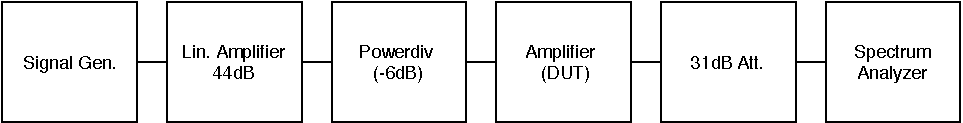
\includegraphics[scale = 0.9]{figures/measurement/cree/meas1/meas_set_1.pdf}
\caption{Measurement setup for measurement at only the amplifier }
\label{fig:meas_amp}
\end{figure}


\begin{figure}[H]
\centering 
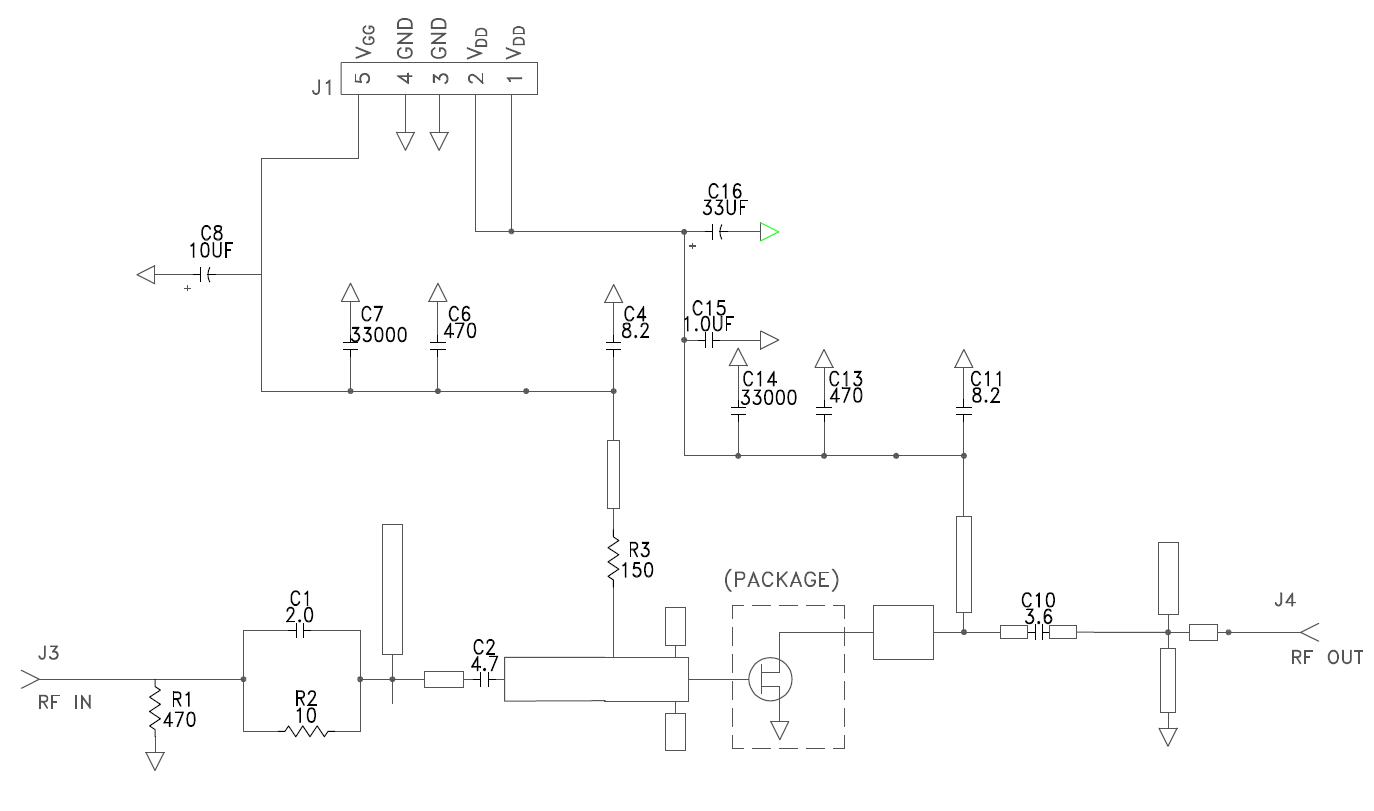
\includegraphics[scale = 0.4]{figures/measurement/cree/cree_schematic.png}
\caption{Schematic of the amplifier board (PACKAGE) is the GaN HEMT transistor. \citep{cree2019}}
\label{fig:meas_amp_sch}
\end{figure}


\begin{figure}[H]
\centering 
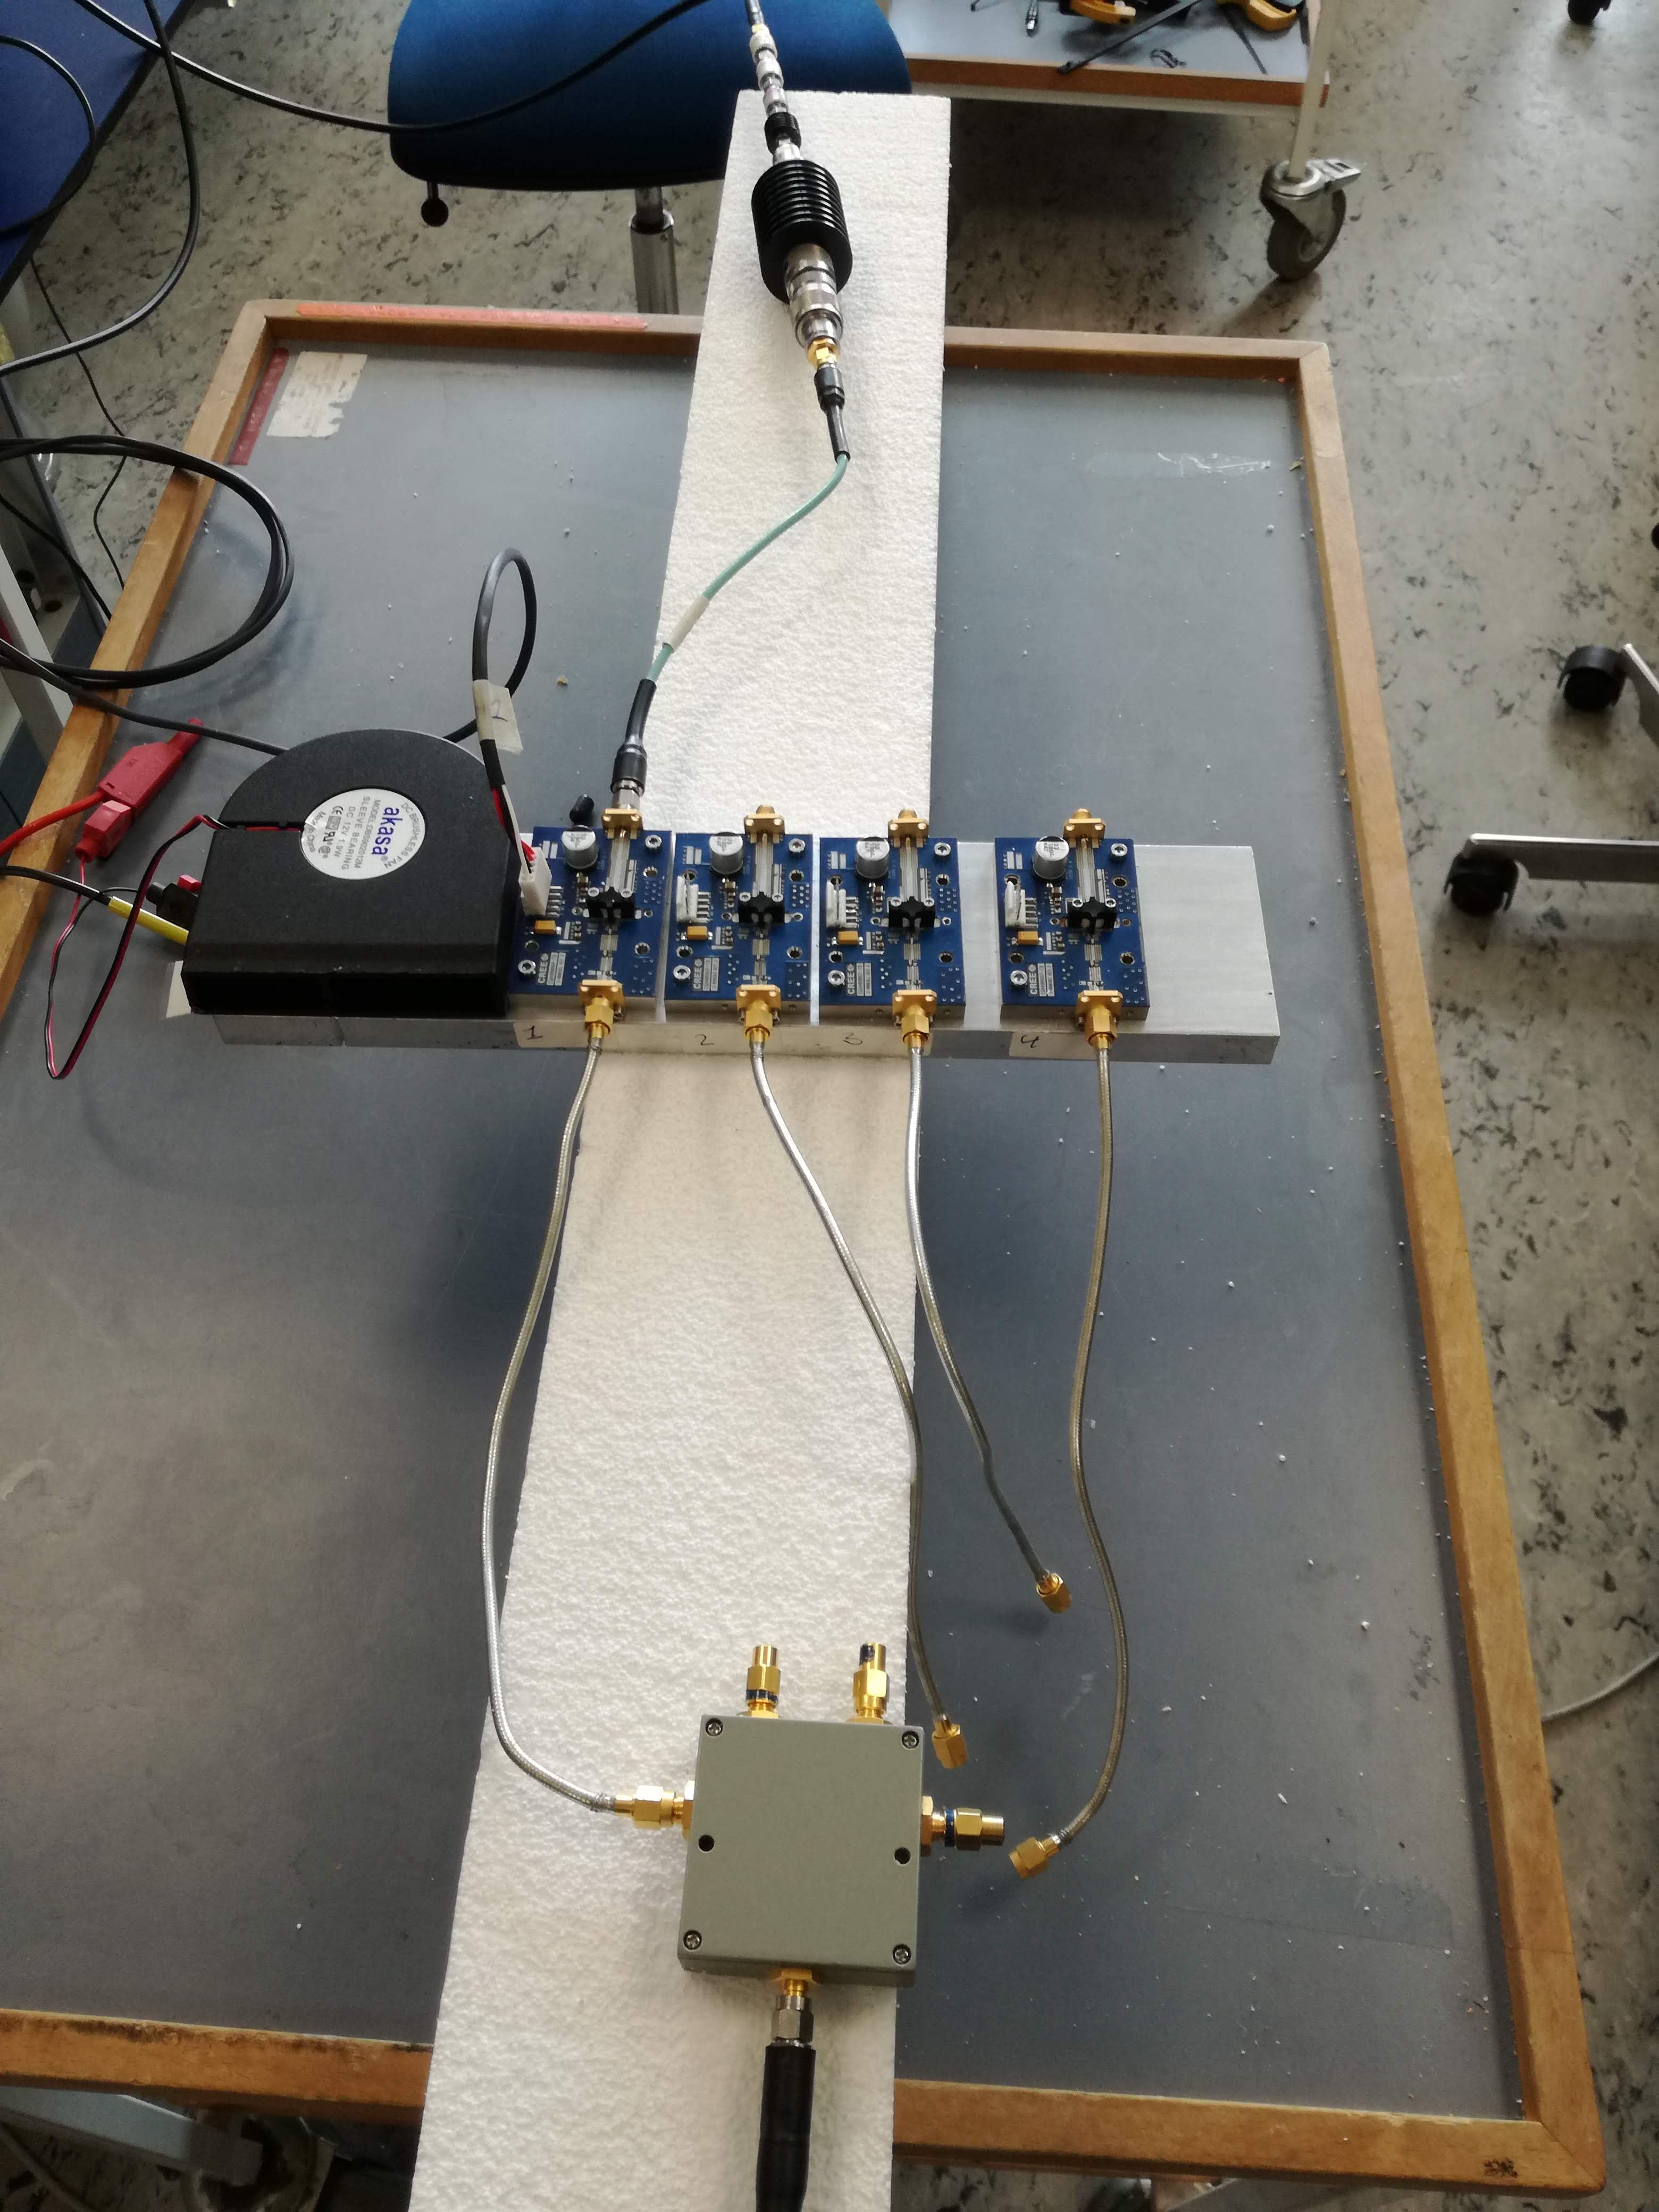
\includegraphics[scale = 0.1]{figures/measurement/cree/meas1/meas_set_1.jpg}
\caption{Picture of the mesurement setup }
\label{fig:meas_amp_pic}
\end{figure}
 

In order to use DPD at the amplifier, it is important to drive the amplifier at its 1dB compression point or more. Therfore the first measurement that has to be done is to measure the gain response of the amplifier to find the input power level that satisfies this. The gate voltage for the amplifier is $V_g = -2.798V$ and the drain current is $I_d = 100mA$. The result are depicted in figure \ref{fig:meas_amp_response}.   

\begin{figure}[H]
\centering 
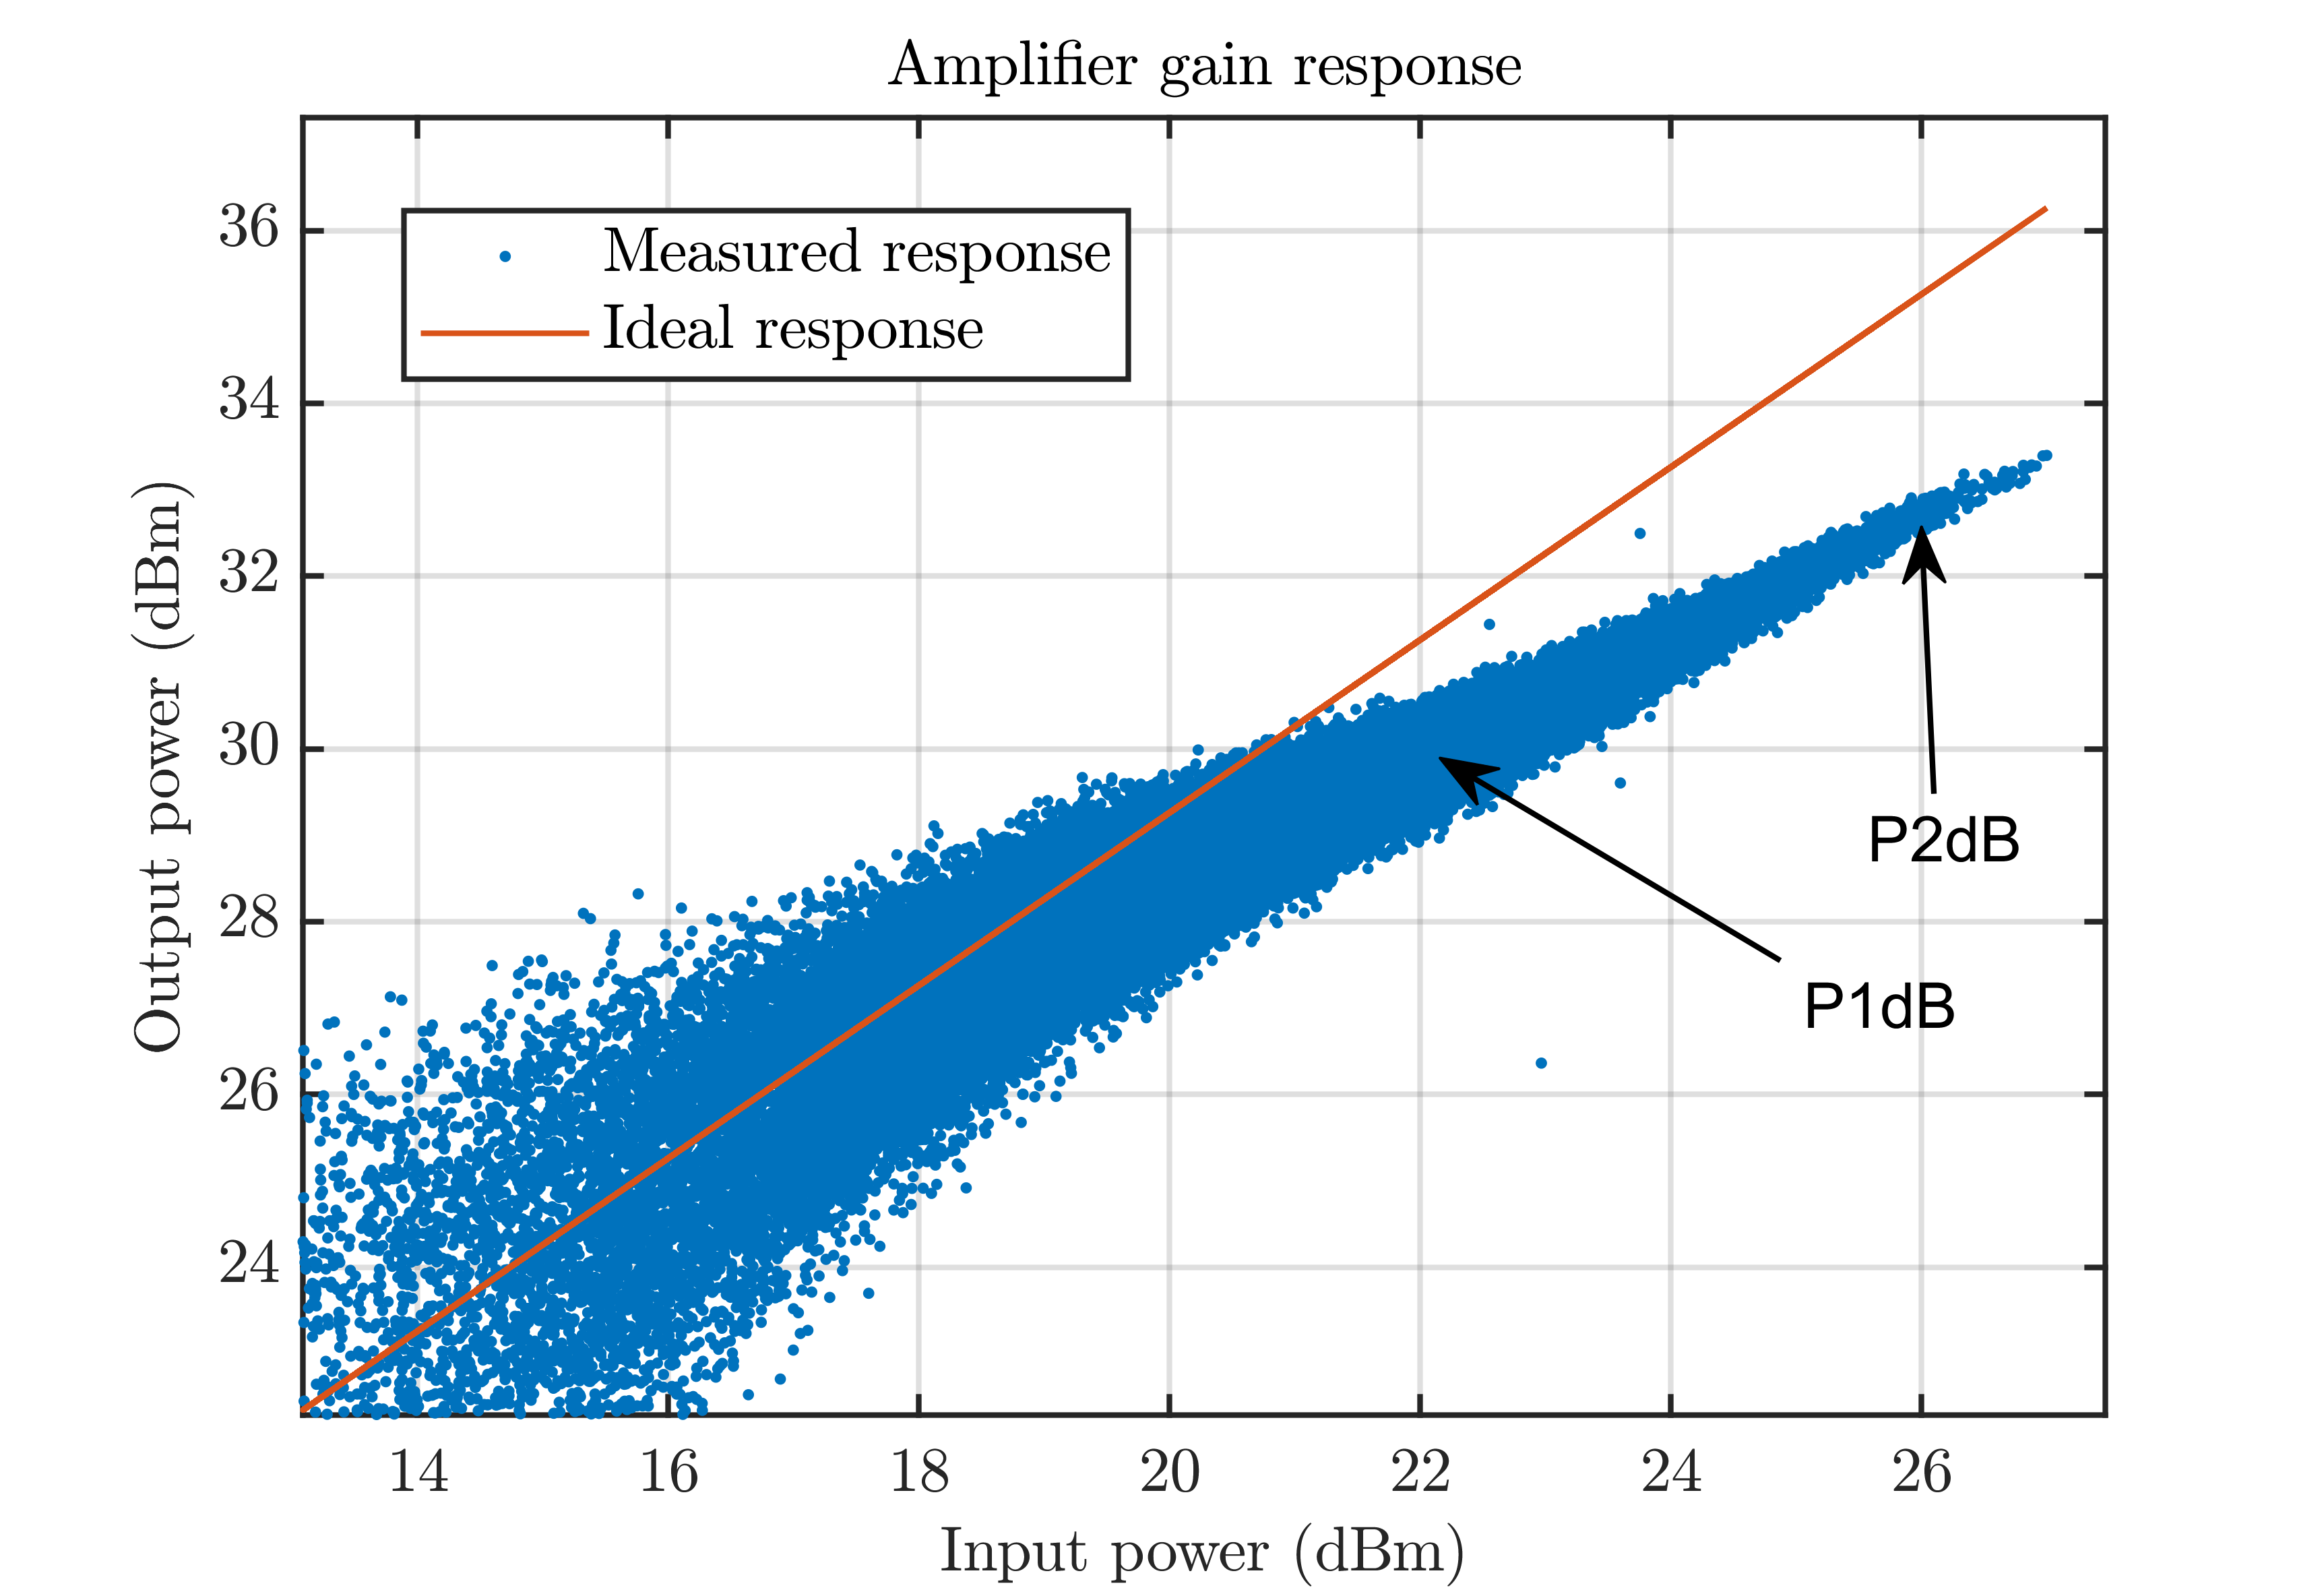
\includegraphics[scale = 0.7]{figures/measurement/cree/meas1/gainResponse.png}
\caption{Measured gain response of the amplifier with a 10MHz LTE signal at 3.5GHz}
\label{fig:meas_amp_response}
\end{figure}

It can be seen from figure \ref{fig:meas_amp_response} that the amplifier in this setup,has a gain about 10dB. The 1dB compresion point is at 22dBm input power and 2dB compression is at 26dBm. Is is therefore decided to continue with a power level that has a peak input power of 27dBm. The DPD algorithm has therefore been applied and the result can be seen in figure \ref{fig:meas_amp_amam} and \ref{fig:meas_amp_PSD}. It can be seen that the DPD works fine and that the distortion becomes lower with the DPD as expected. It can be seen from the AM/AM plot that the gain is lowered to 9dB with the DPD but that compression is avoided. 

\begin{figure}[H]
\centering 
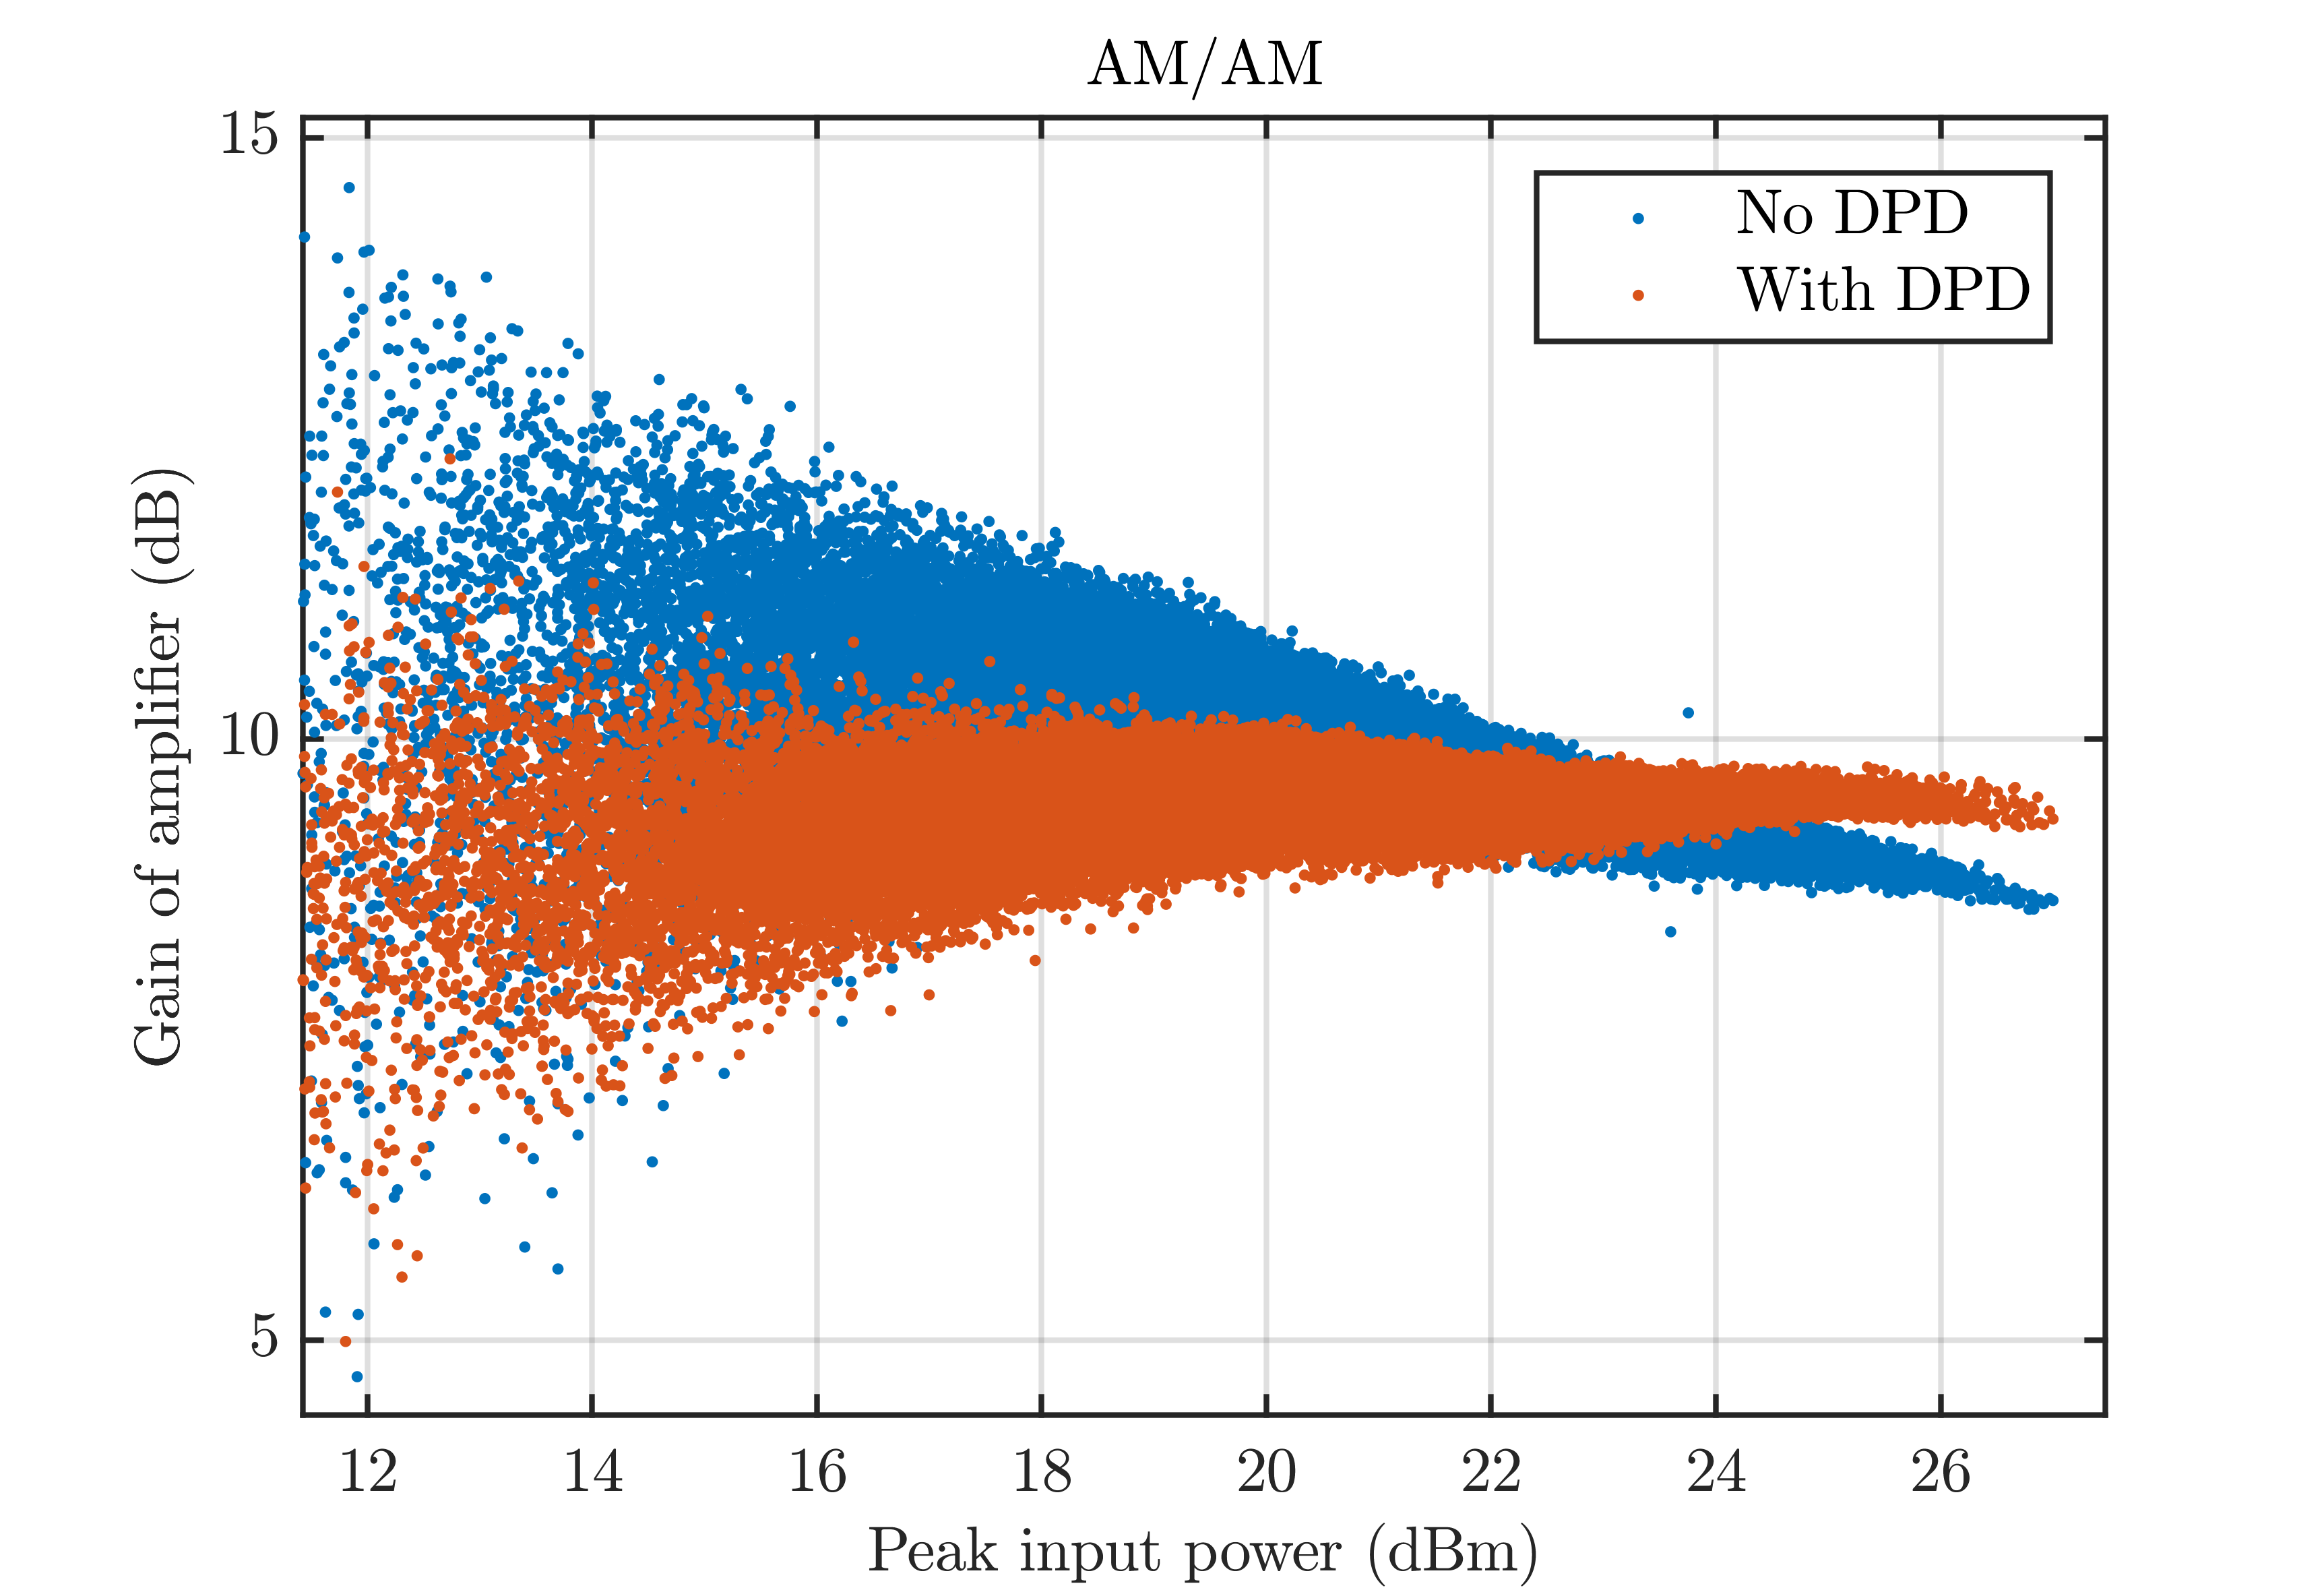
\includegraphics[scale = 0.7]{figures/measurement/cree/meas1/AMAM.png}
\caption{AM/AM response of the amplifier with and without DPD}
\label{fig:meas_amp_amam}
\end{figure}


\begin{figure}[H]
\centering 
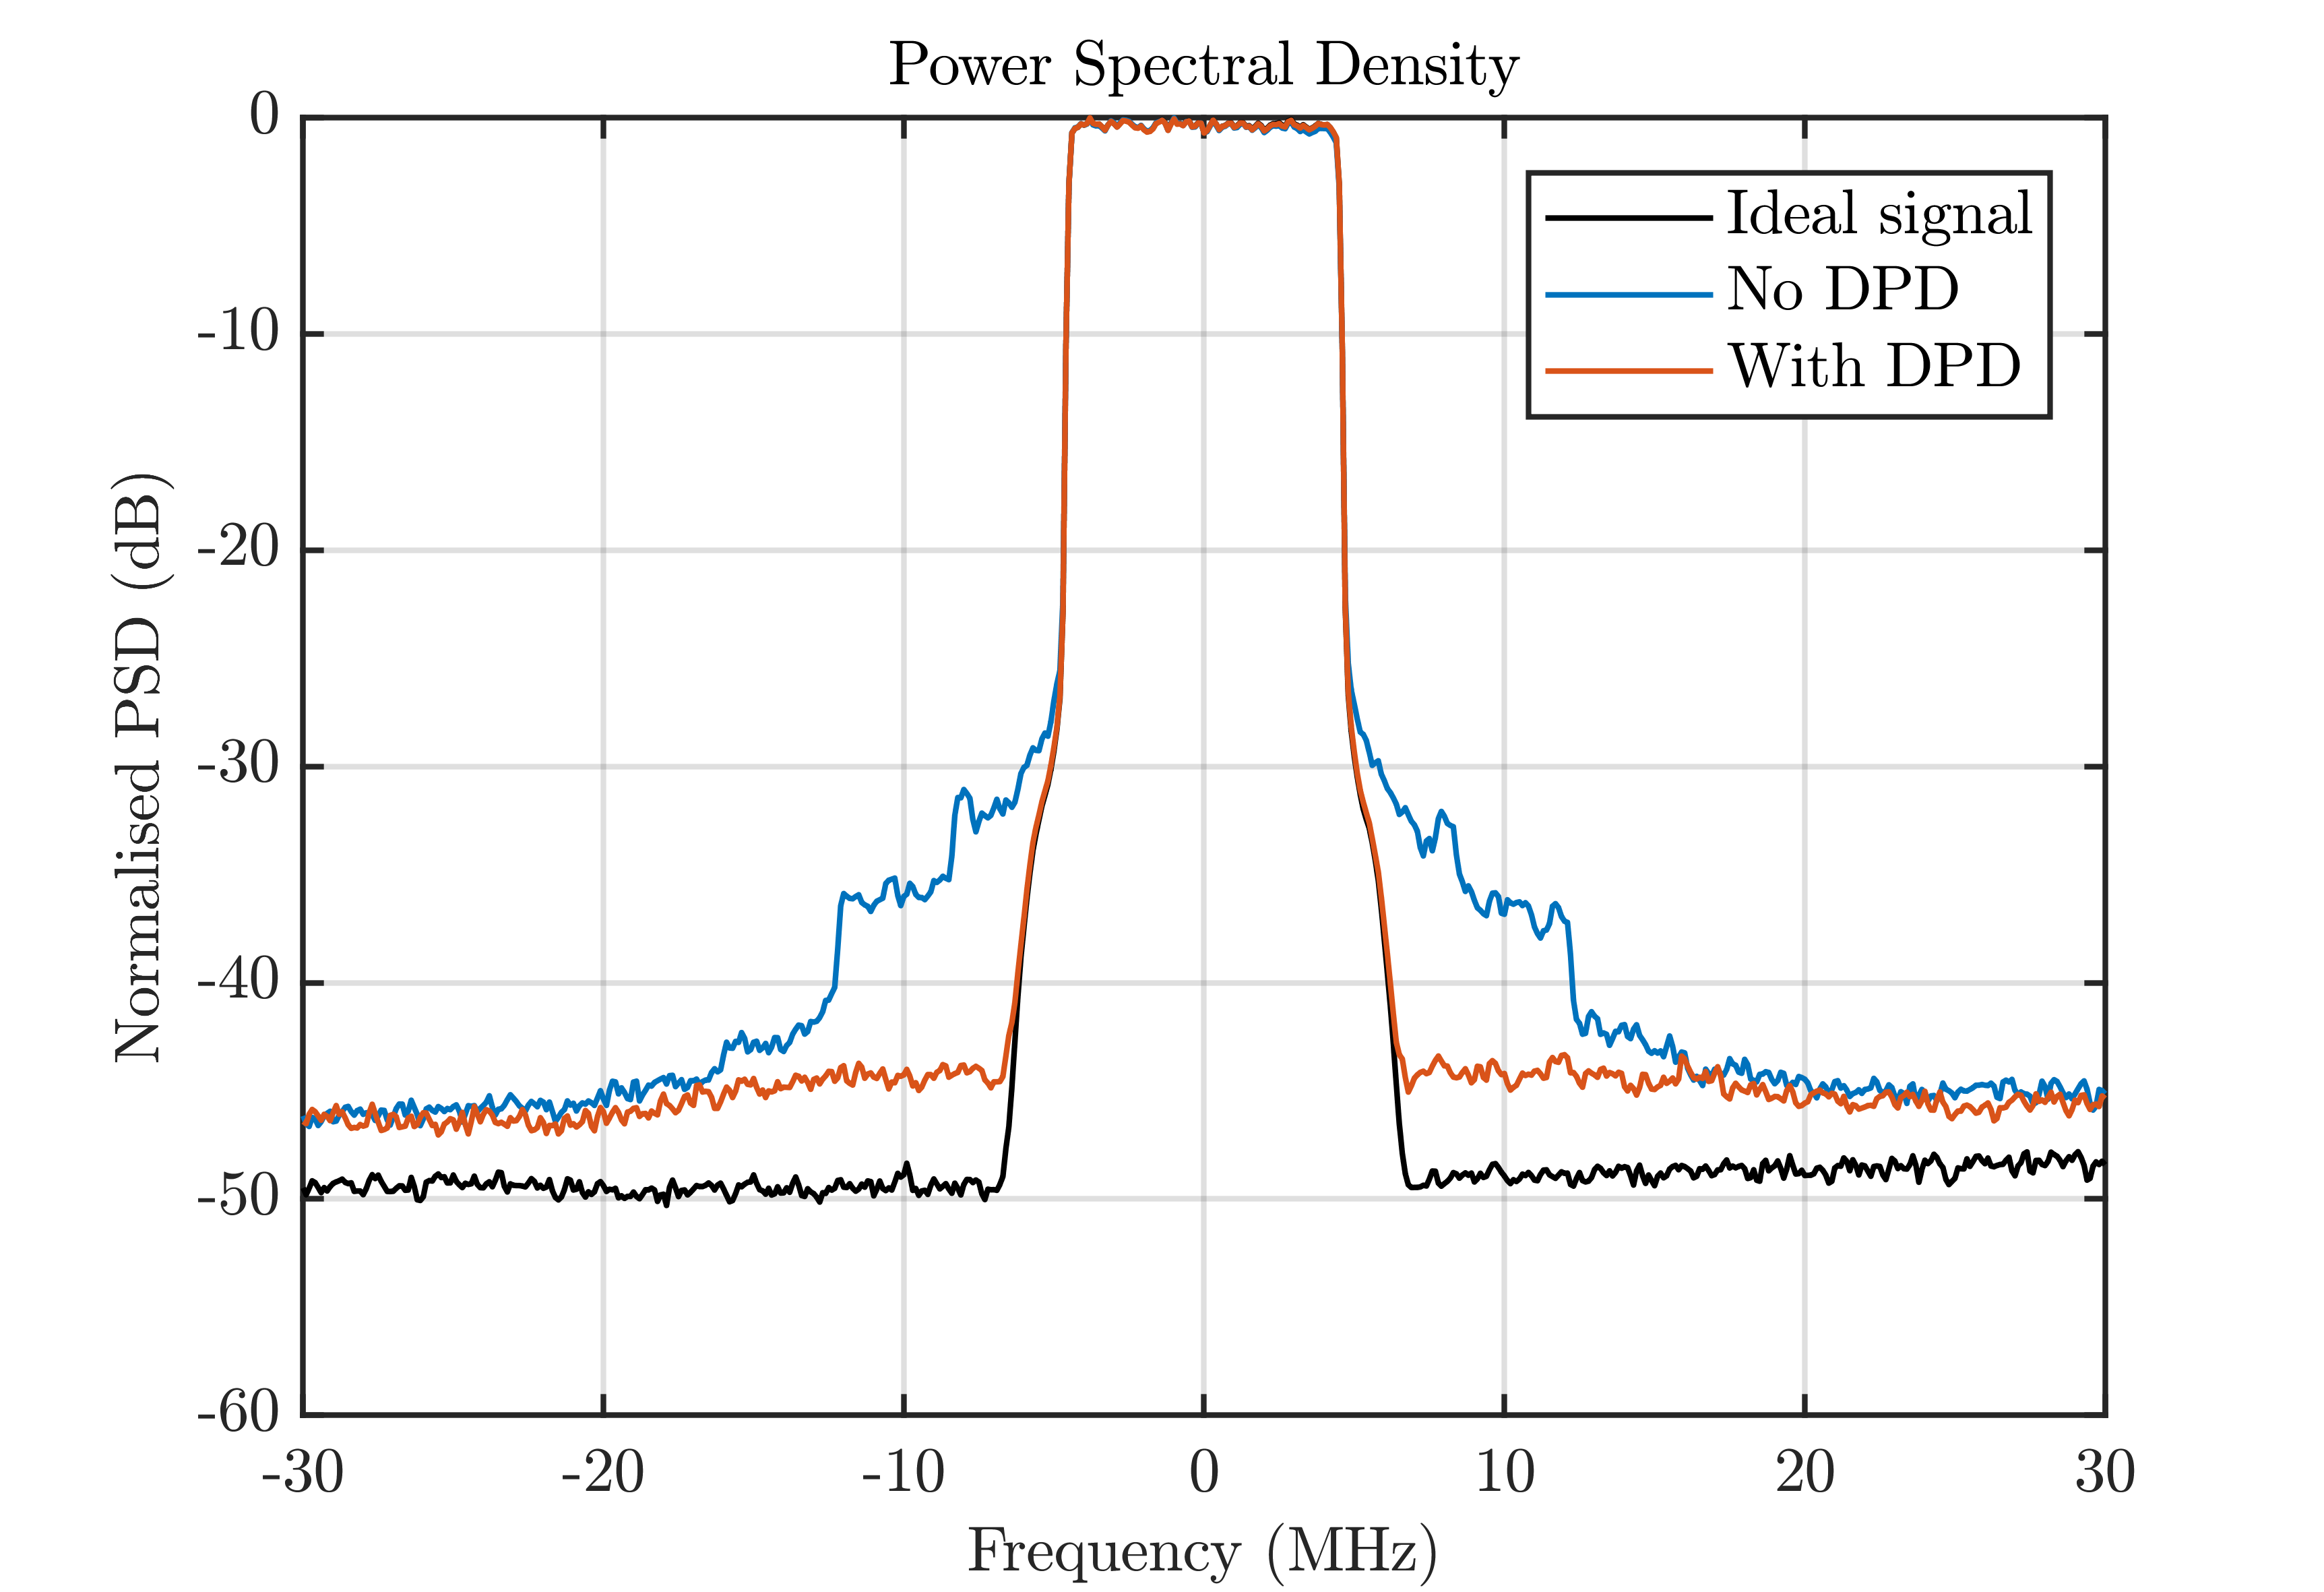
\includegraphics[scale = 0.7]{figures/measurement/cree/meas1/PSD_1.png}
\caption{Measured PSD with and without DPD}
\label{fig:meas_amp_PSD}
\end{figure}

\section{One amplifier one antenna}

\begin{figure}[H]
\centering 
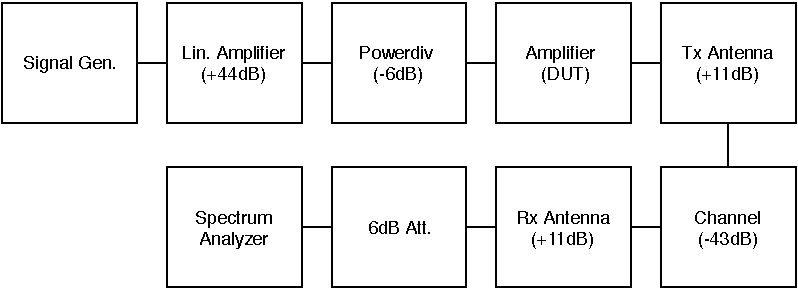
\includegraphics[scale = 0.9]{figures/measurement/cree/meas2/meas2.pdf}
\caption{Measurement setup for measurement at one amplifier with one Tx and one Rx antenna}
\label{fig:meas_amp2}
\end{figure}

Since now it has been proven that the DPD works well for a single amplifier connected to a fixed load, it is necessary to see if there would be any changes when the amplifier is connected to a single Tx antenna. The measurement setup is depicted in figure \ref{fig:meas_amp2}. The output of the amplifier is connected to one Tx antenna with a gain at 11dB. The Rx antenna are spaced 1m apart which also has a gain at 11db. The distance between  the antennas gives a loss at 43dB in free space. The total loss can be calculated as:

\begin{equation}
 L_{dB} = 20log_{10}(d)+20log_{10}(f)+20log_{10}(\frac{4\pi}{c})+G_t+G_r = 21.3dB
\end{equation}
Where $d$ is distance between the antennas, $f$ is the center frequency, $c=3.0e8$ is the speed of light and $G_t$ $G_r$ is the gain of the transmitting antenna and receiving antenna respectively \citep{Balanis2005}. In order to compensate for the loss and to drive the spectrum analyser in the same power level as in the former measurement, the attenuator has been reduced to 6dB. It is seen from figure \ref{fig:meas_amp2_amam} that the gain now is close to 10dB which is not exact the same as before but close. The error is caused by the compensation for the free space loss that is not fully correct. The distortion seen in figure \ref{fig:meas_amp2_PSD} is lowered with DPD and therfore it can be concluded that the DPD still works with one antenna connected to the amplifier. The model used for DPD is the model for the amplifier only. In next section the antennas are taken into account before the DPD linke in figure \ref{fig:dpd_pdpd}.      


\begin{figure}[H]
\centering 
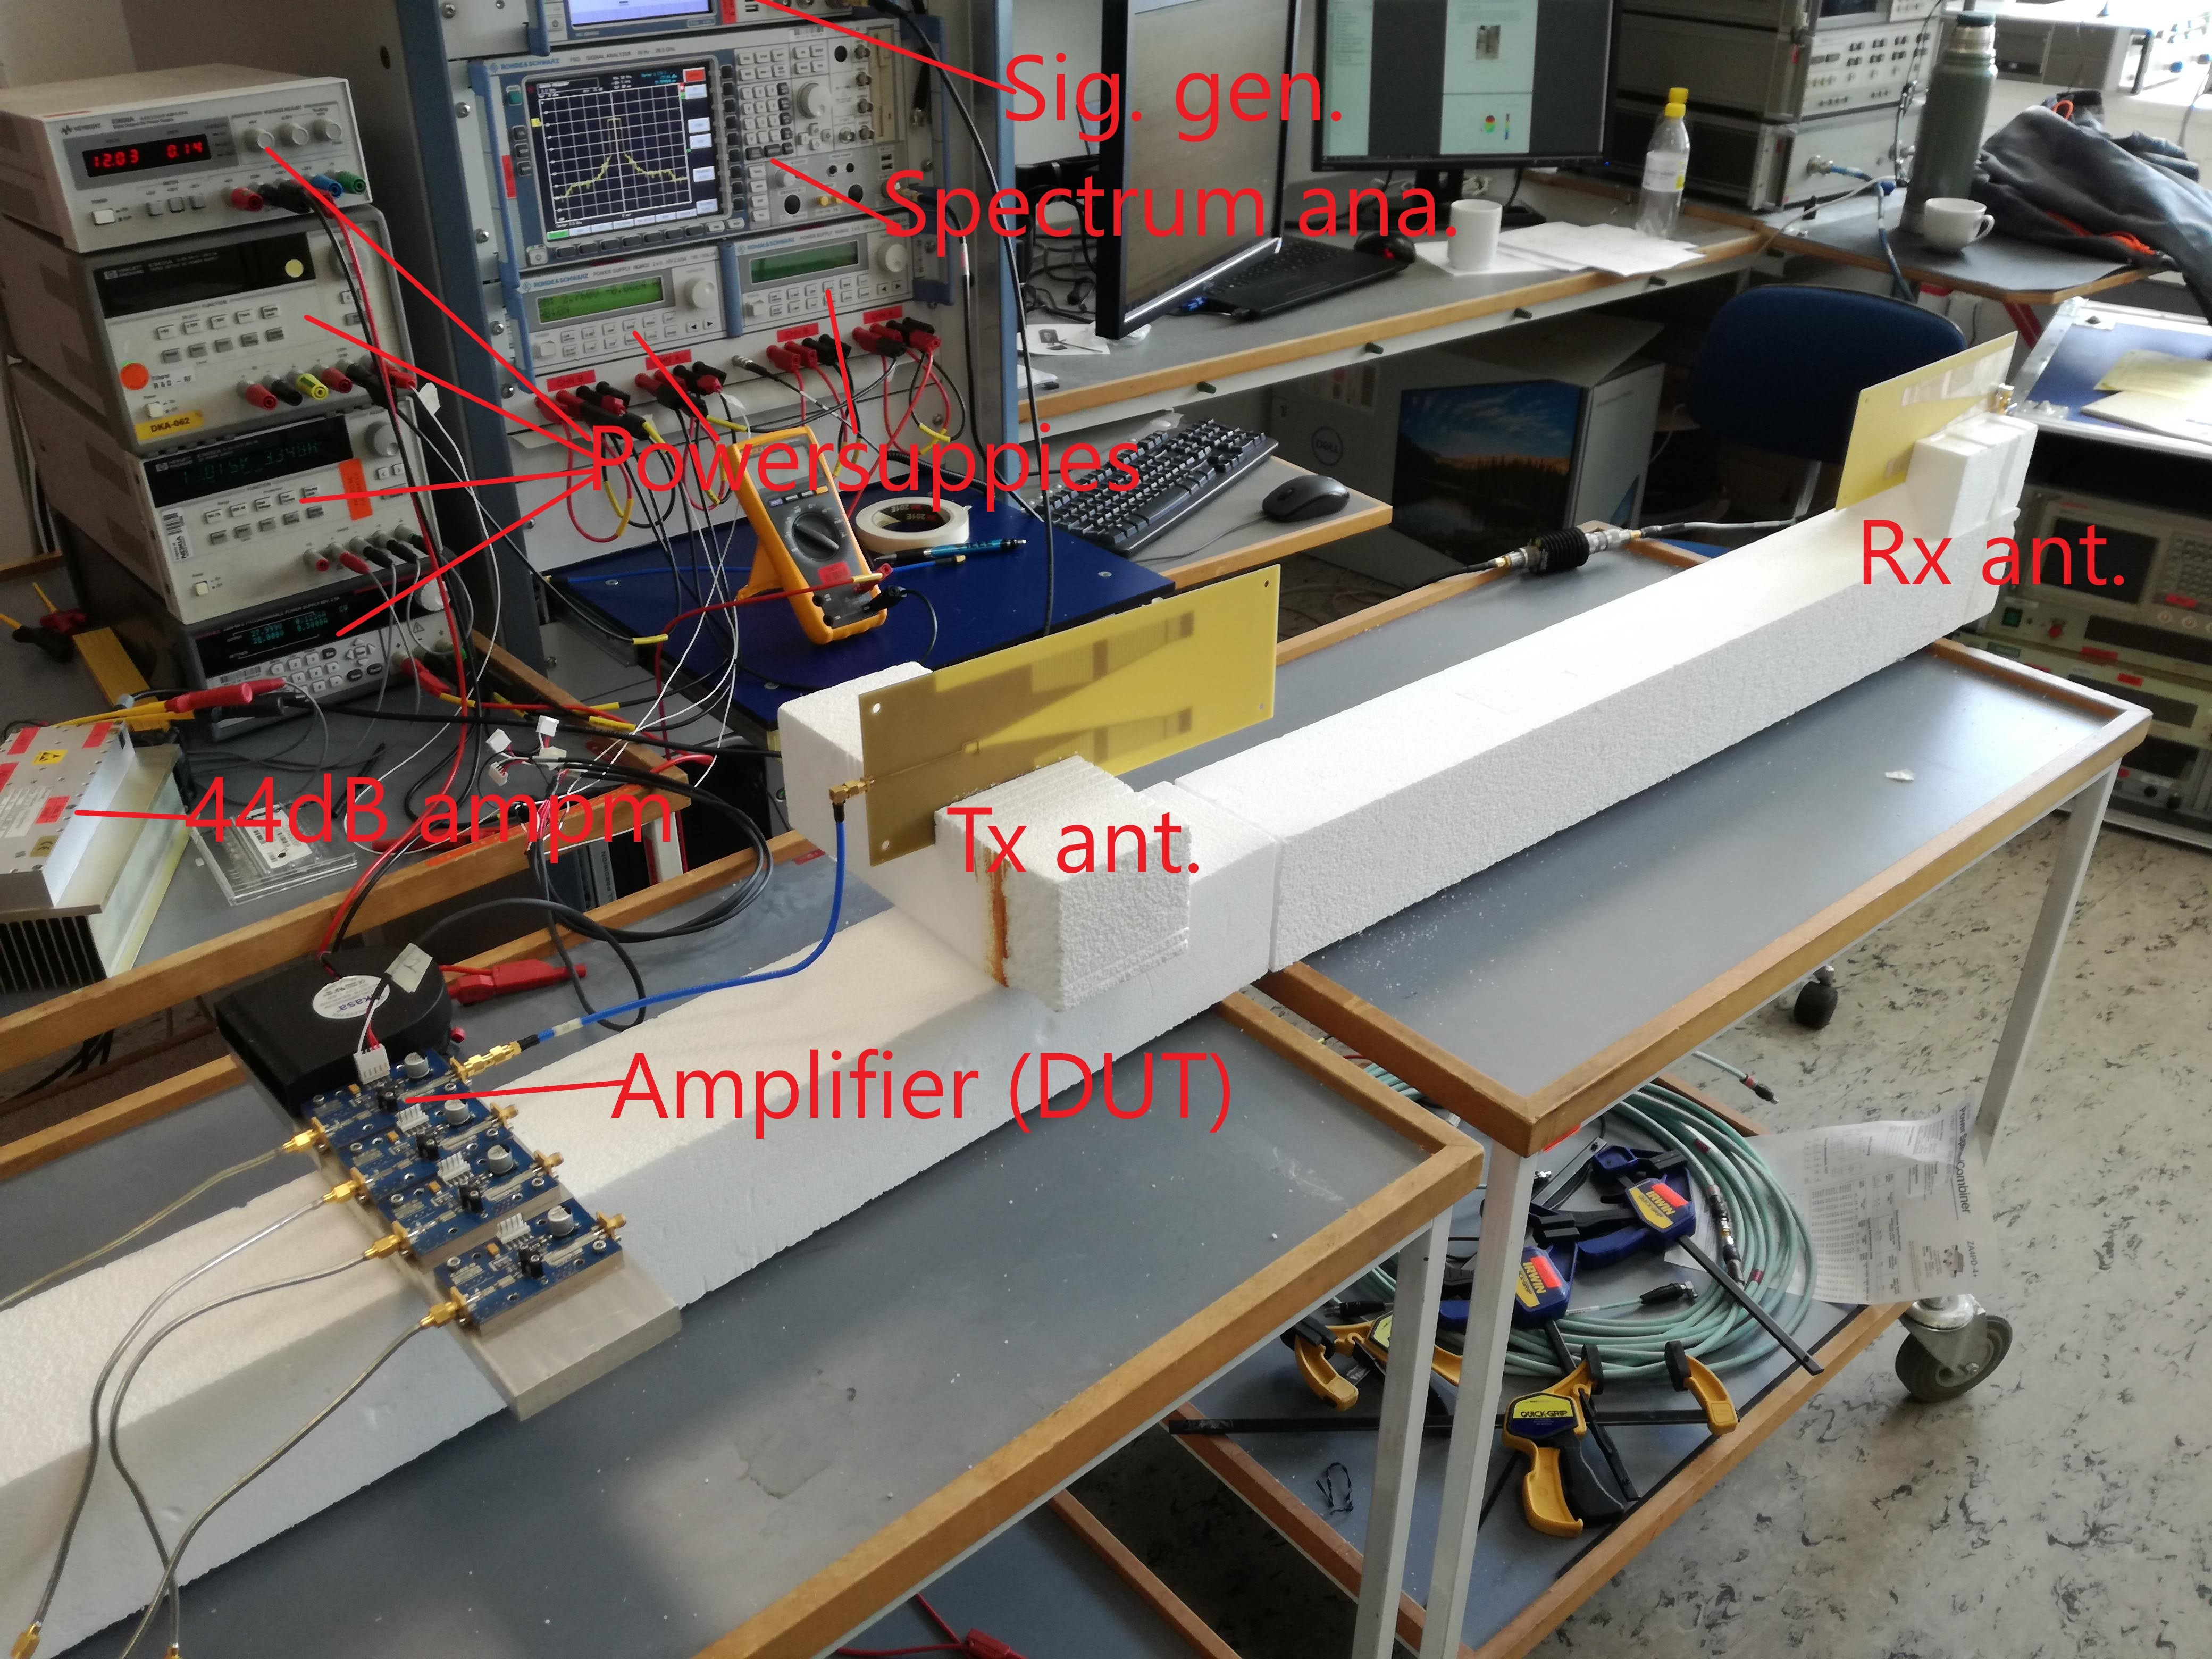
\includegraphics[scale = 0.1]{figures/measurement/cree/meas2/meas2.jpg}
\caption{Picture of the mesurement setup for one amplifier with one Tx and one Rx antenna }
\label{fig:meas_amp2_pic}
\end{figure}



\begin{figure}[H]
\centering 
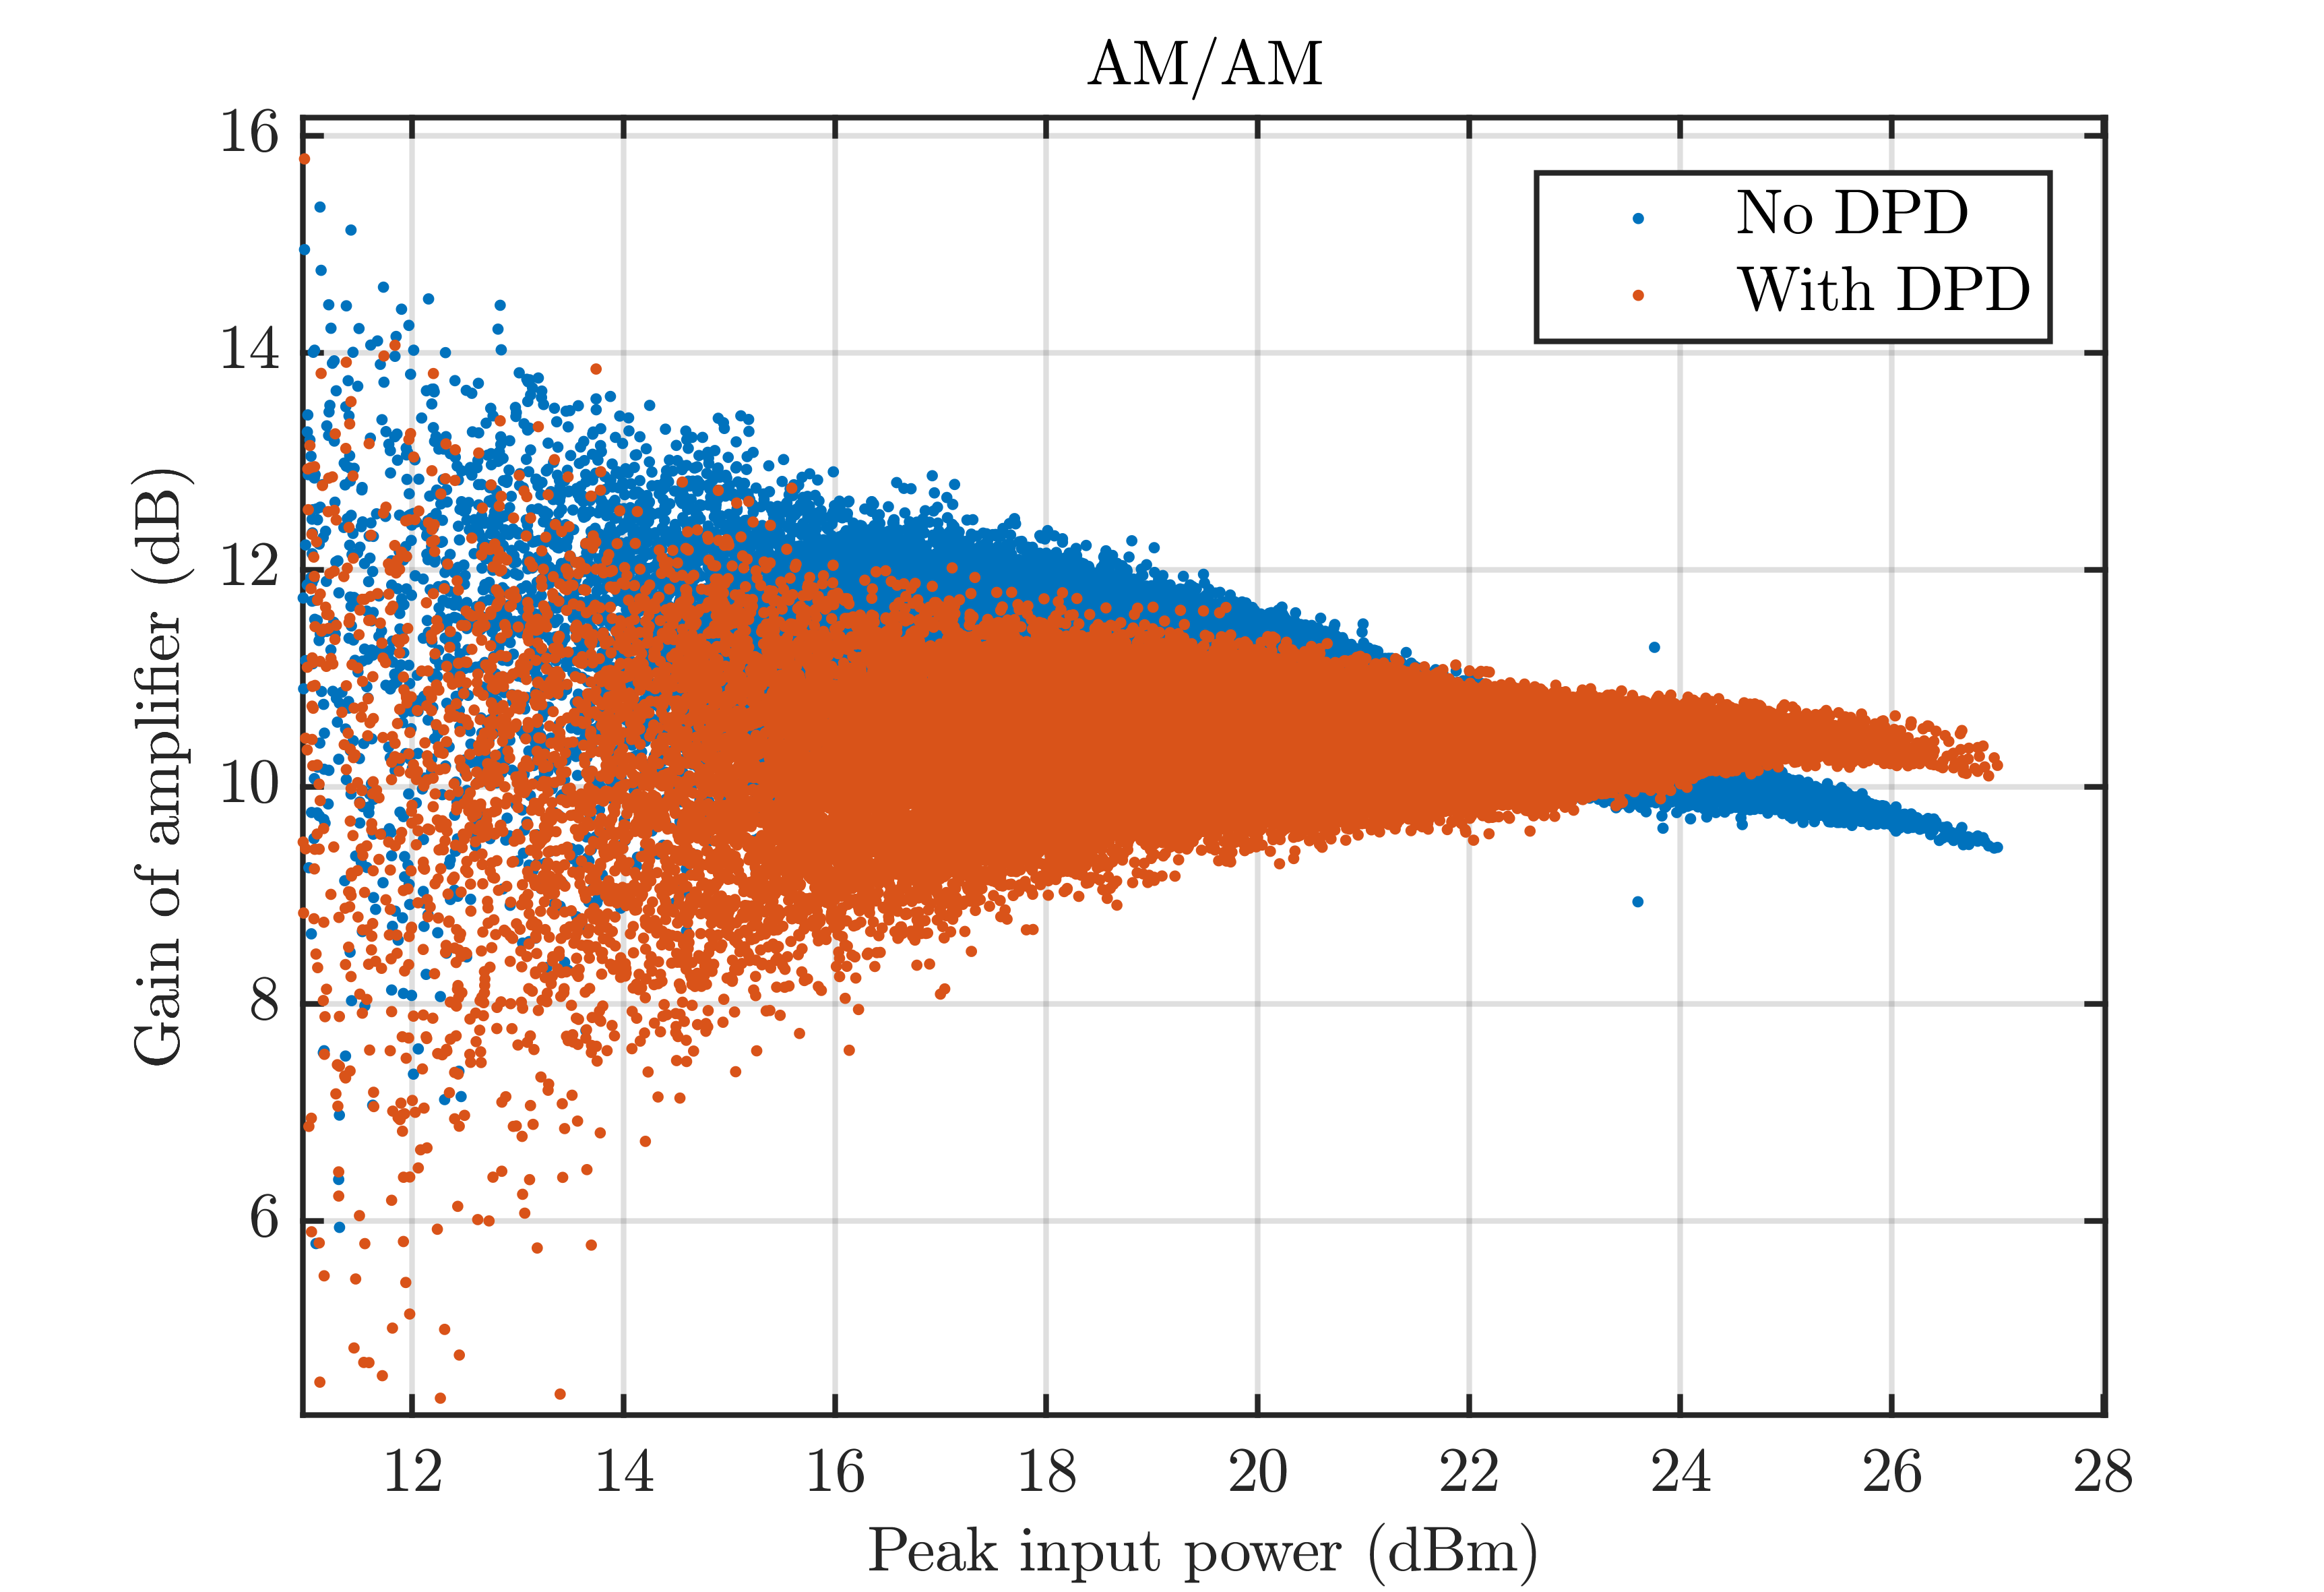
\includegraphics[scale = 0.7]{figures/measurement/cree/meas2/AMAM.png}
\caption{AM/AM response of the amplifier with and without DPD using one Tx antenna}
\label{fig:meas_amp2_amam}
\end{figure}


\begin{figure}[H]
\centering 
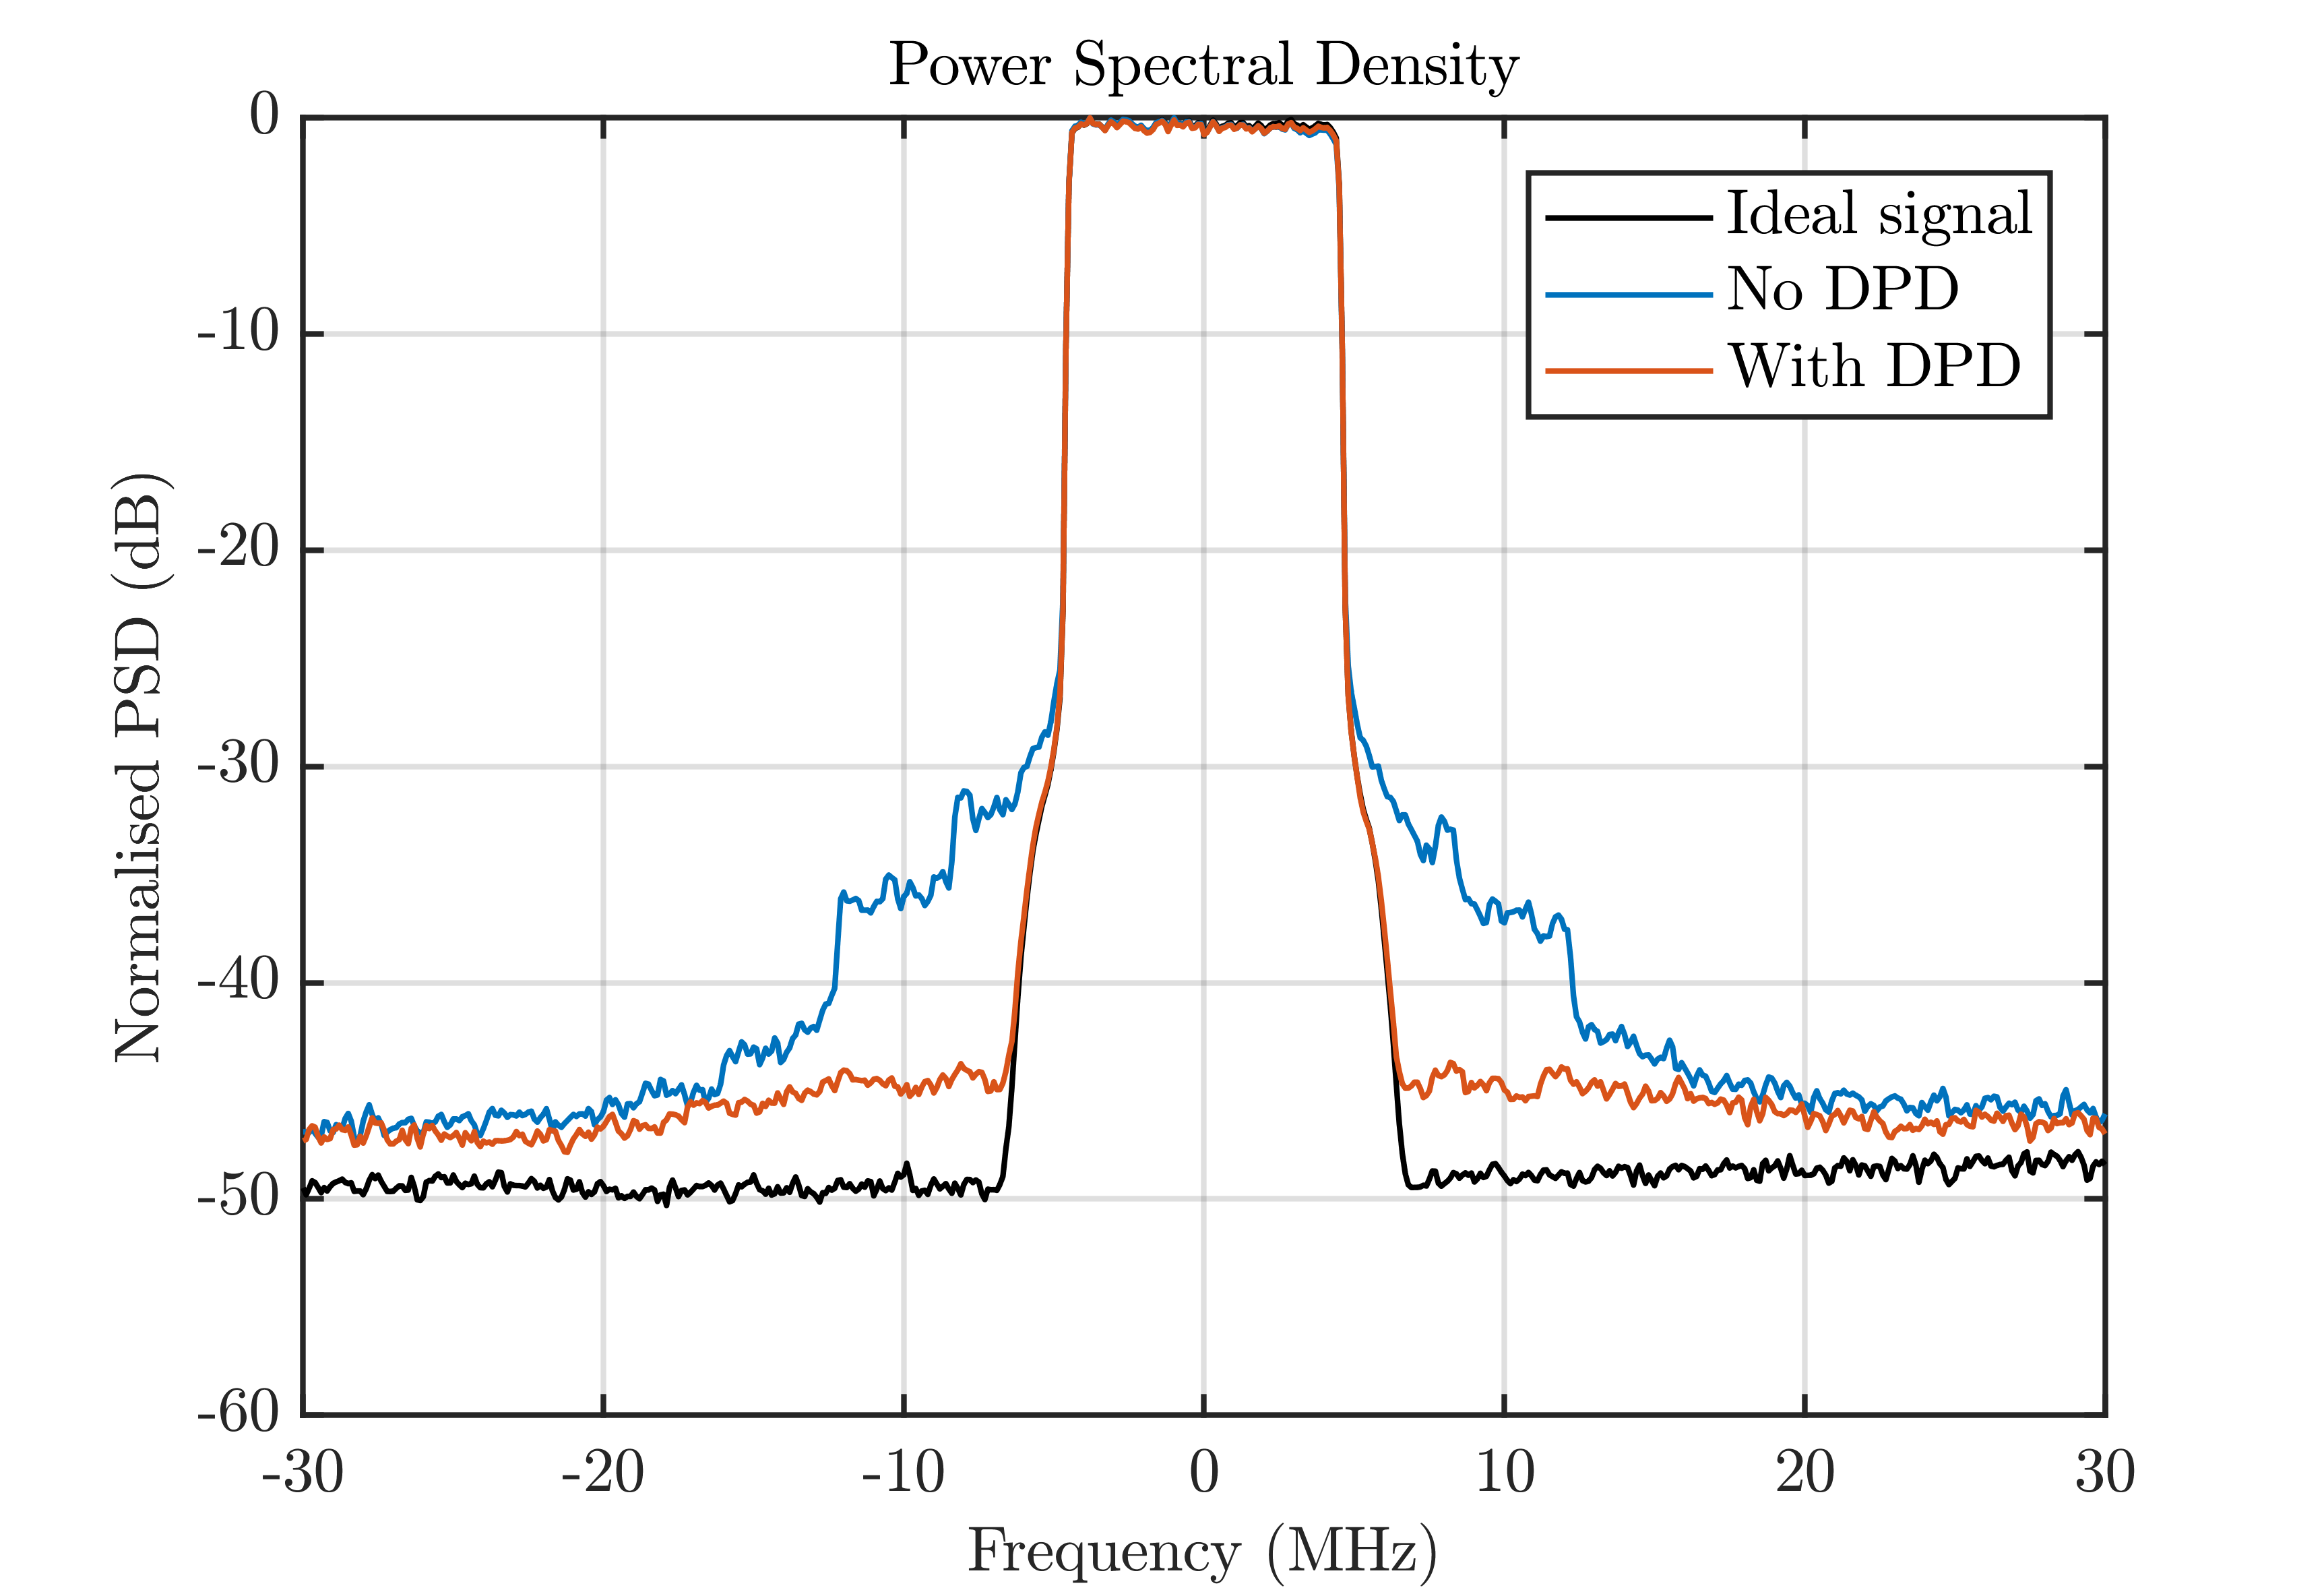
\includegraphics[scale = 0.7]{figures/measurement/cree/meas2/PSD.png}
\caption{Measured PSD with and without DPD using one Tx antenna}
\label{fig:meas_amp2_PSD}
\end{figure}


%%%%%%%%%%%%%%%%%%%%%%%%%%%%%%%%%%%%%%%%%%%%%%%%%%%%%%%%%%%%%%%%%%%%%%%%%%%%%%%%%%%%%%%%%%%%%%%%%%%%%%%%%%%%%%%%%%%%
\section{Two amplifiers two antennas}

\begin{figure}[H]
\centering 
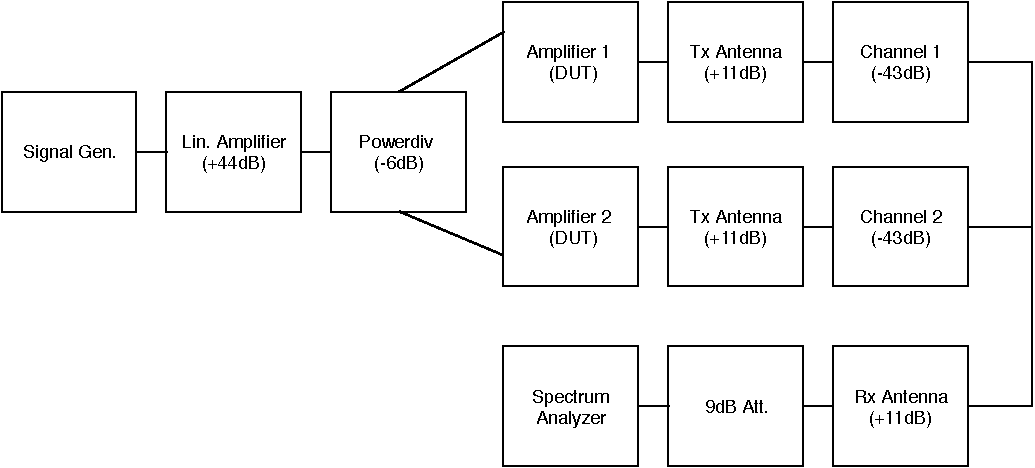
\includegraphics[scale = 0.9]{figures/measurement/cree/meas3/meas3.pdf}
\caption{Measurement setup for measurement at two amplifiers with two Tx and one Rx antenna}
\label{fig:meas_amp3}
\end{figure}

In this section it is measured if it has an impact if two amplifiers are connected to an antenna each, spaced at different distances. The measurement setup is depicted in figure \ref{fig:meas_amp3}. Since the extra amplifier and antenna will introduce 3dB more power, 3dB is added to the attenuator to ensure the same power level at the input to the spectrum analyzer. The measurements has all been done at the same powerlevel but the distances of the antennas are varied from 0.1 wavelength to 0.6 in steps of 0.1. First a measurement of the system is done without DPD for all distances, where the measured signal is imported into MATLAB and an inverse signal is generated. This inverse signal is then uploaded to the signal generator and the new measurement is called "With sys DPD" for each distance. Then a meausrement with the inverse signal from the former section is applied for each distance and the measured signal is then called "With amp DPD".The results can be seen from figure \ref{fig:meas3_amam1} to \ref{fig:meas3_amam6}.   


\begin{figure}[H]
\centering 
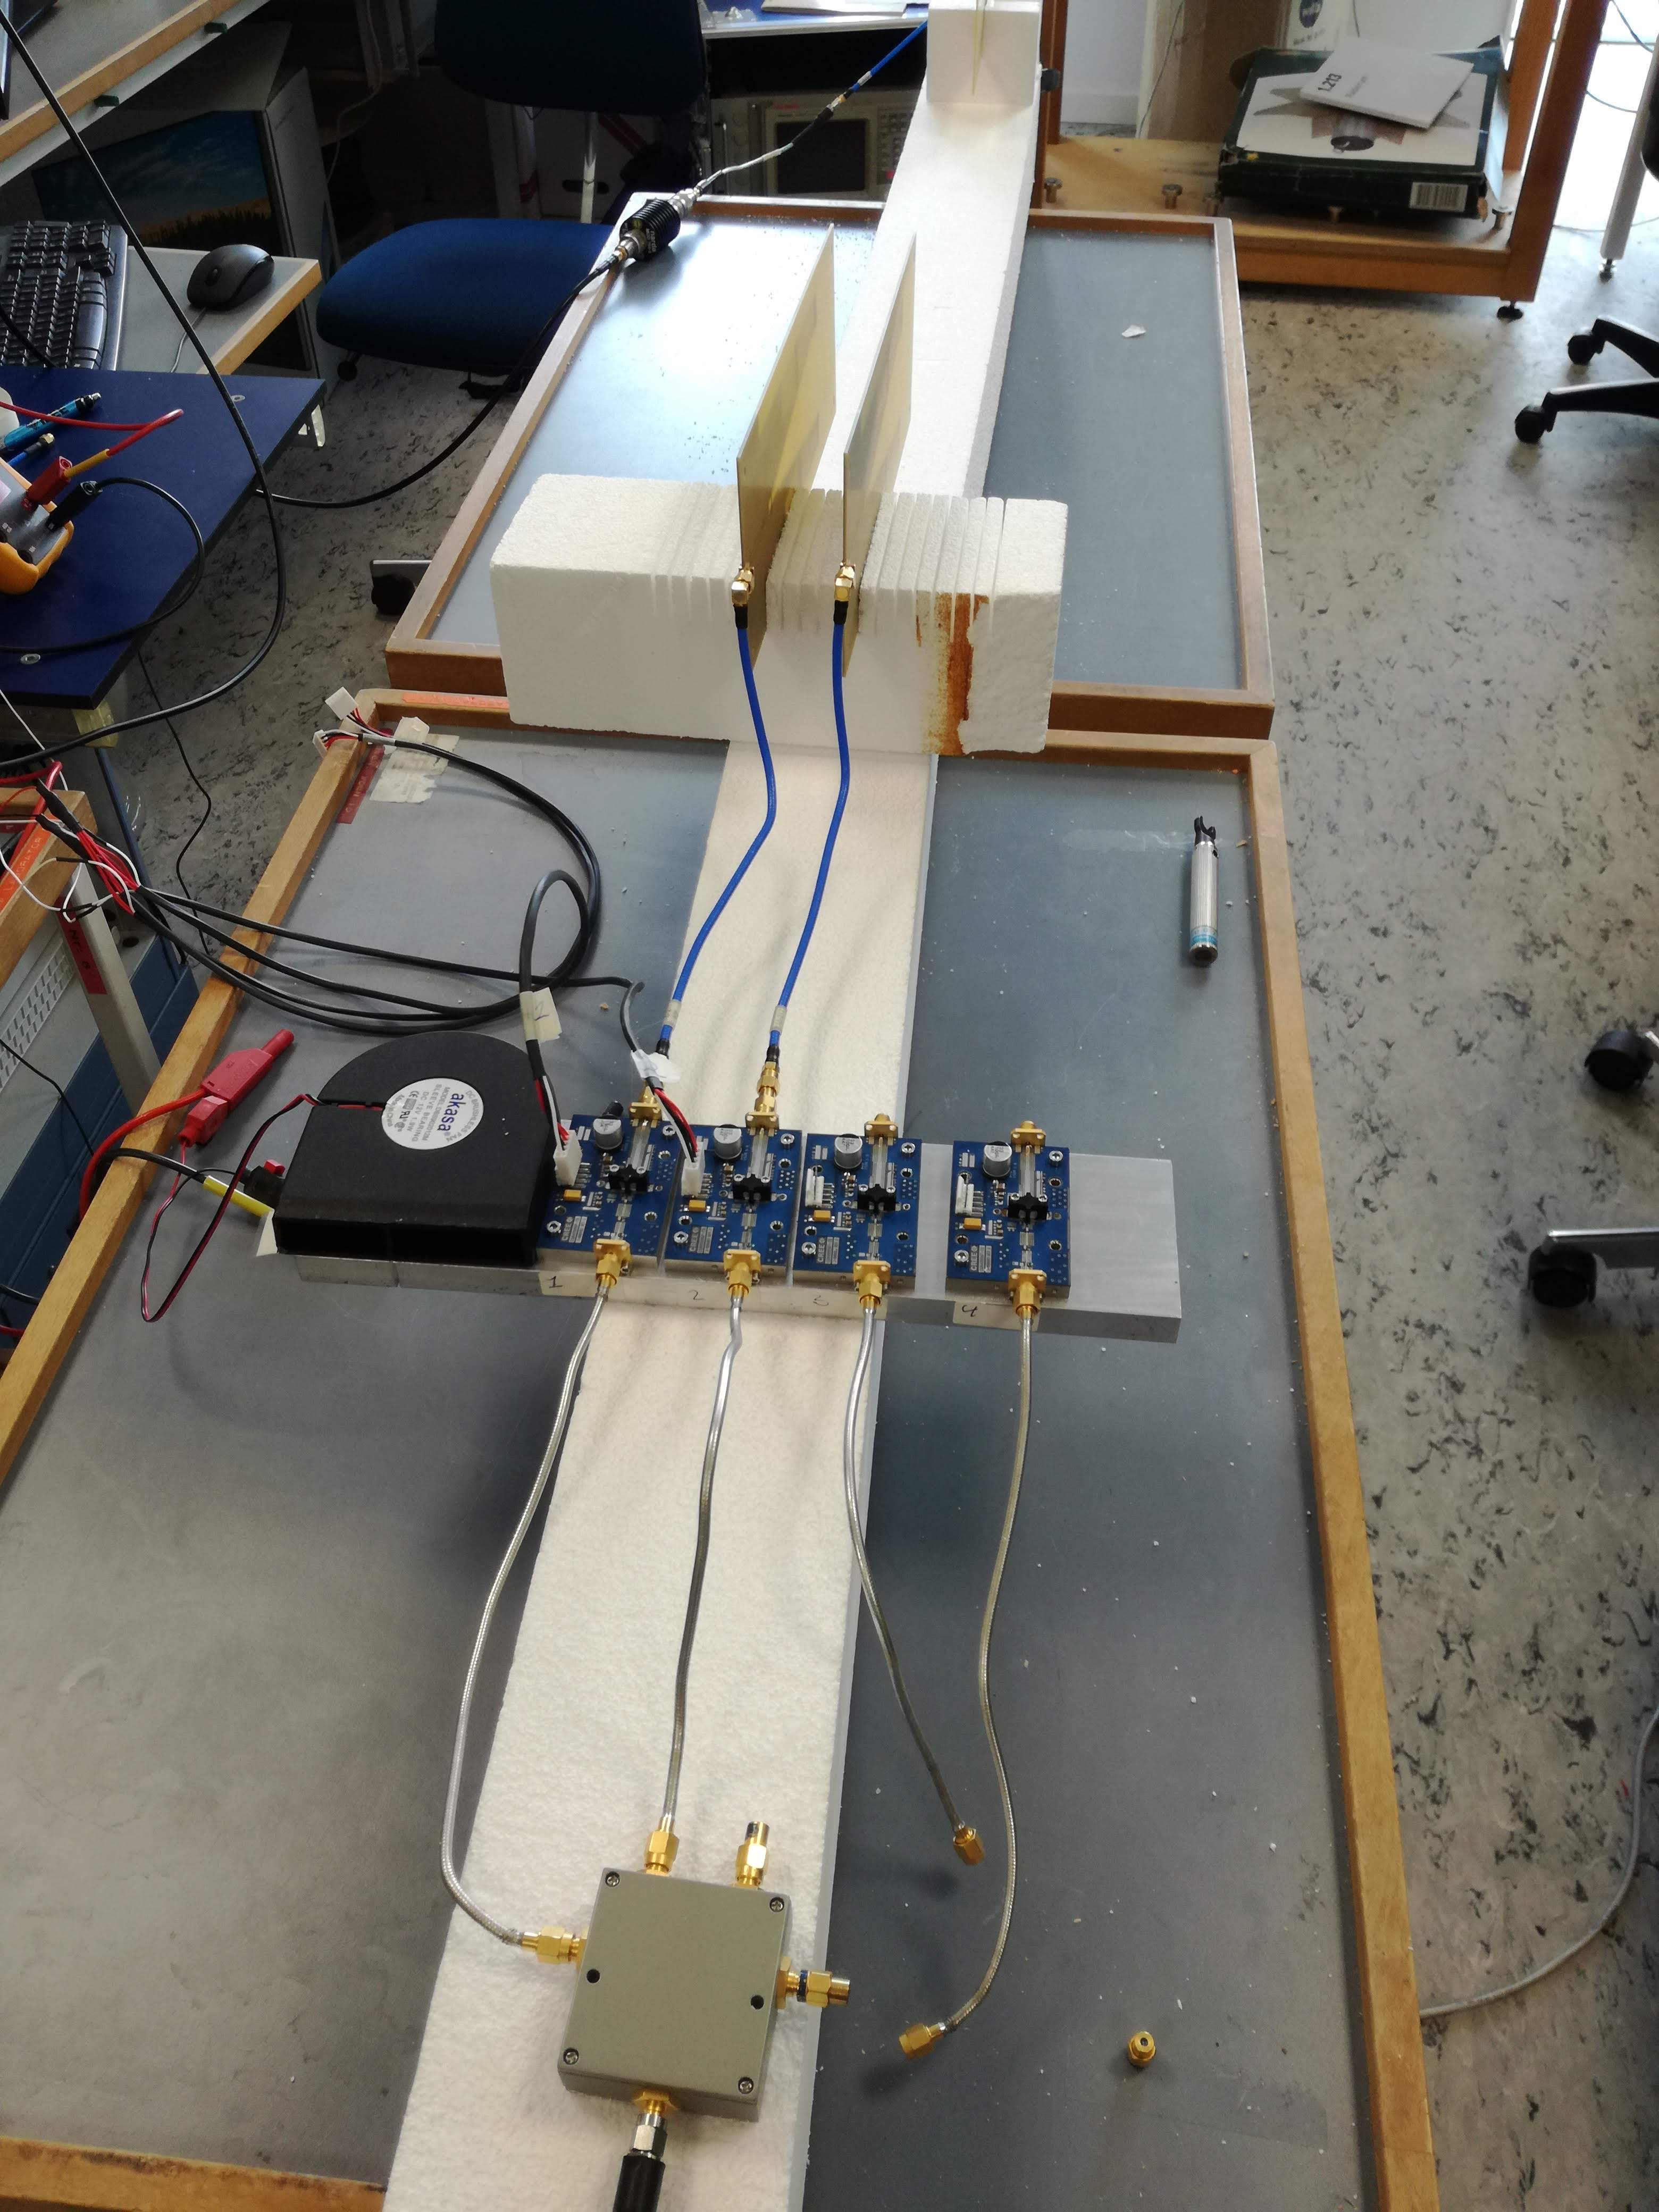
\includegraphics[scale = 0.1]{figures/measurement/cree/meas3/meas3.jpg}
\caption{Picture of measurement setup using two Tx antennas}
\label{fig:meas_amp3-2}
\end{figure}

\begin{figure}[H]
  \centering
  \begin{minipage}[b]{0.5\textwidth}
	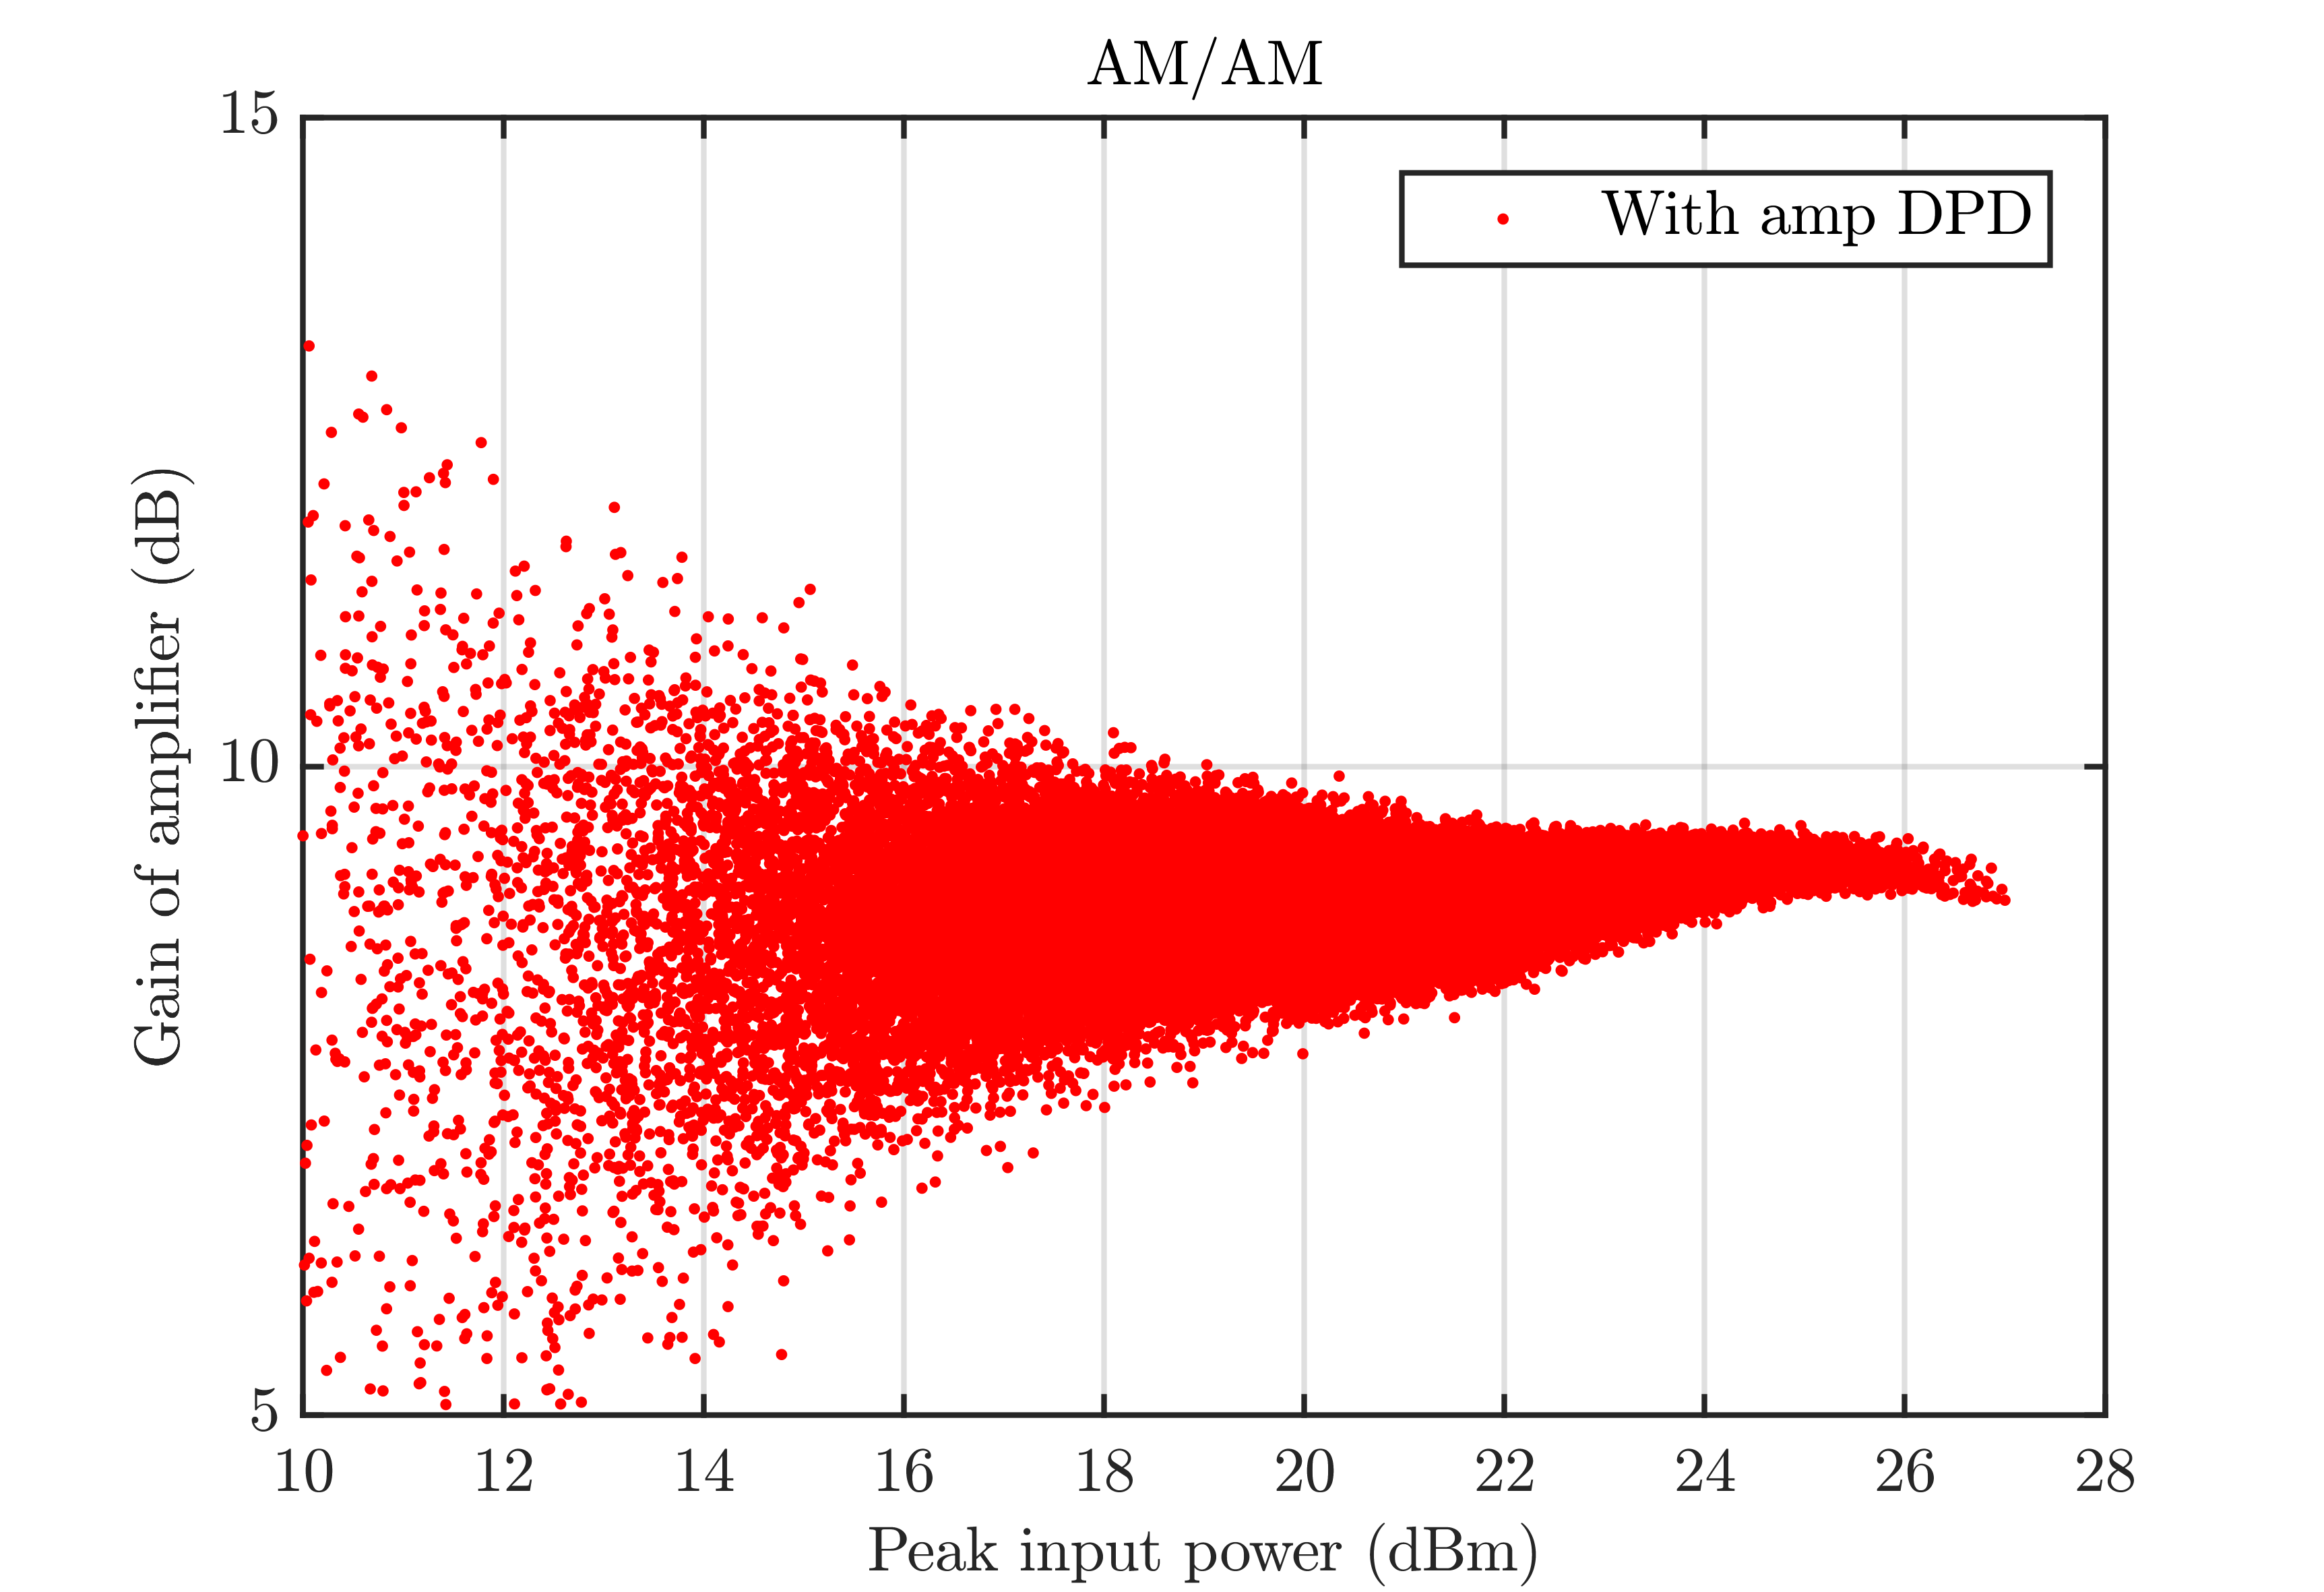
\includegraphics[scale = 0.5]{figures/measurement/cree/meas3/amam_amp_dpd_0p1.png}
	\caption{AM/AM distortion at $d = 0.1\lambda$ with amplifier DPD}	
    \label{fig:meas3_amam1}
  \end{minipage}
  \hfill
  \begin{minipage}[b]{0.4\textwidth}
	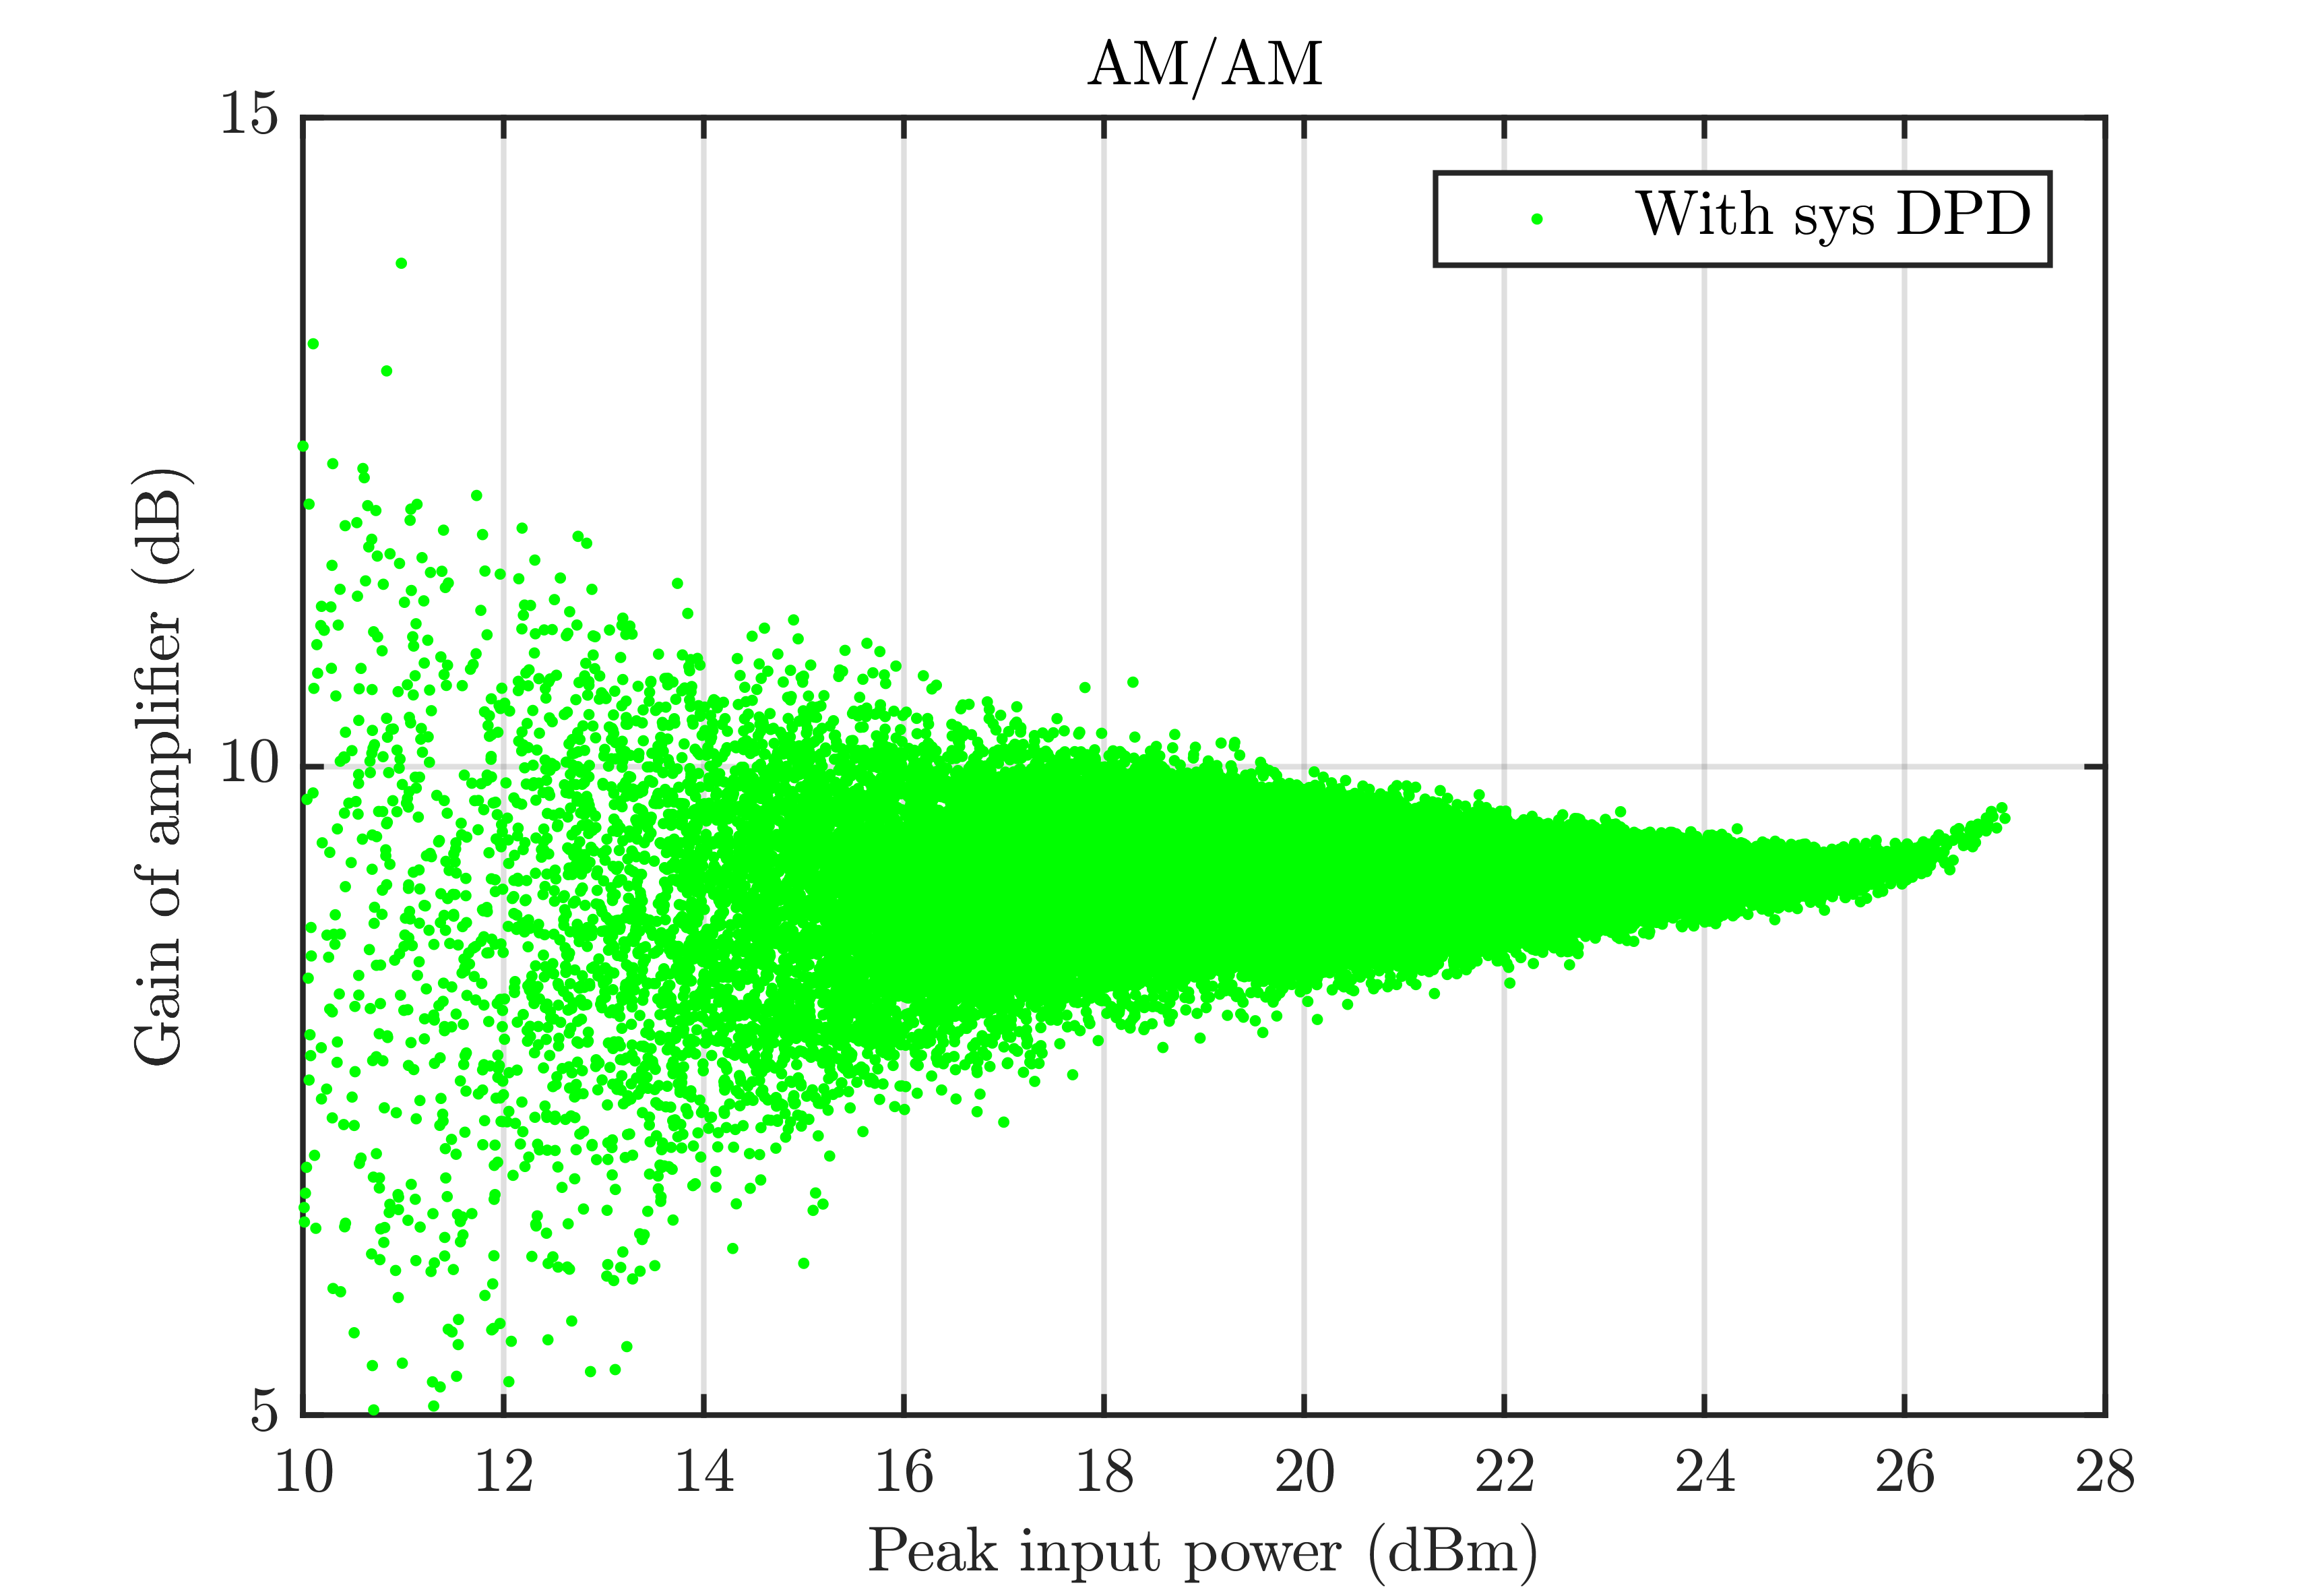
\includegraphics[scale = 0.5]{figures/measurement/cree/meas3/amam_sys_dpd_0p1.png}
	\caption{AM/AM distortion at $d = 0.1\lambda$ with system DPD}
    \label{fig:meas3_amam2}
  \end{minipage}
\end{figure}

\begin{figure}[H]
  \centering
  \begin{minipage}[b]{0.5\textwidth}
	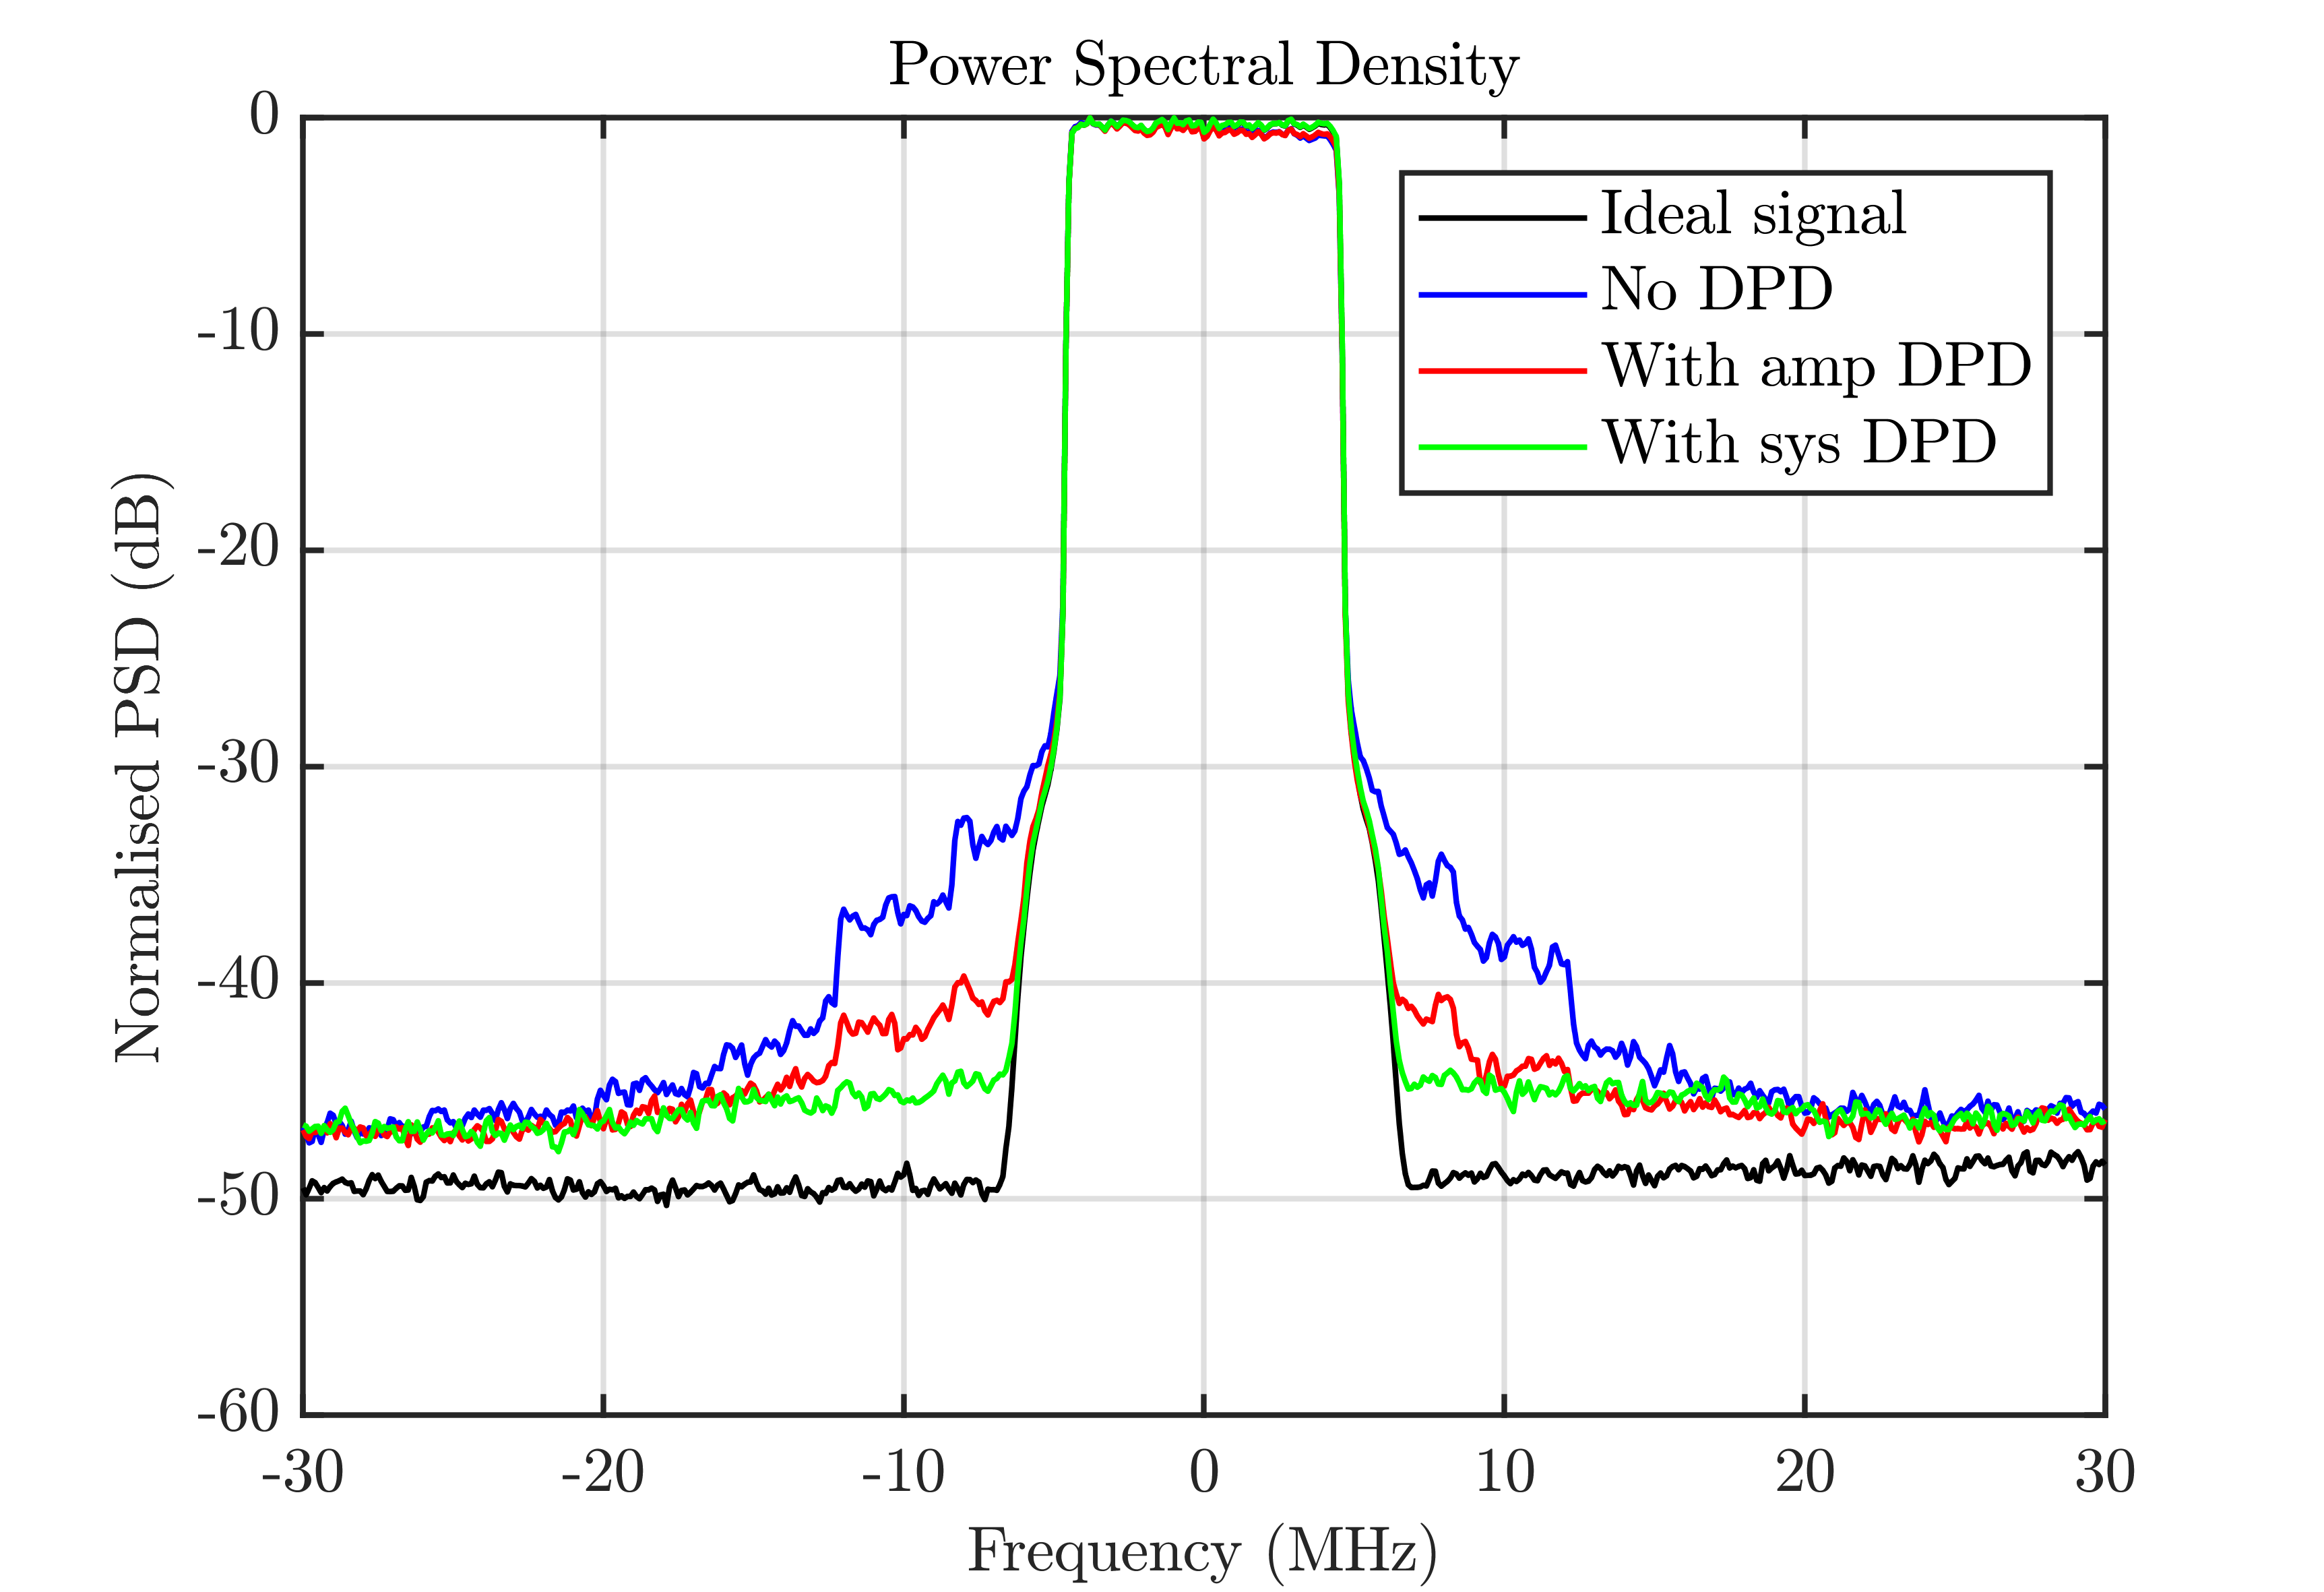
\includegraphics[scale = 0.5]{figures/measurement/cree/meas3/psd_0p1.png}
	\caption{PSD of measurement at $d = 0.1\lambda$ }	
    \label{fig:meas3_psd1}
  \end{minipage}
  \hfill
  \begin{minipage}[b]{0.4\textwidth}
	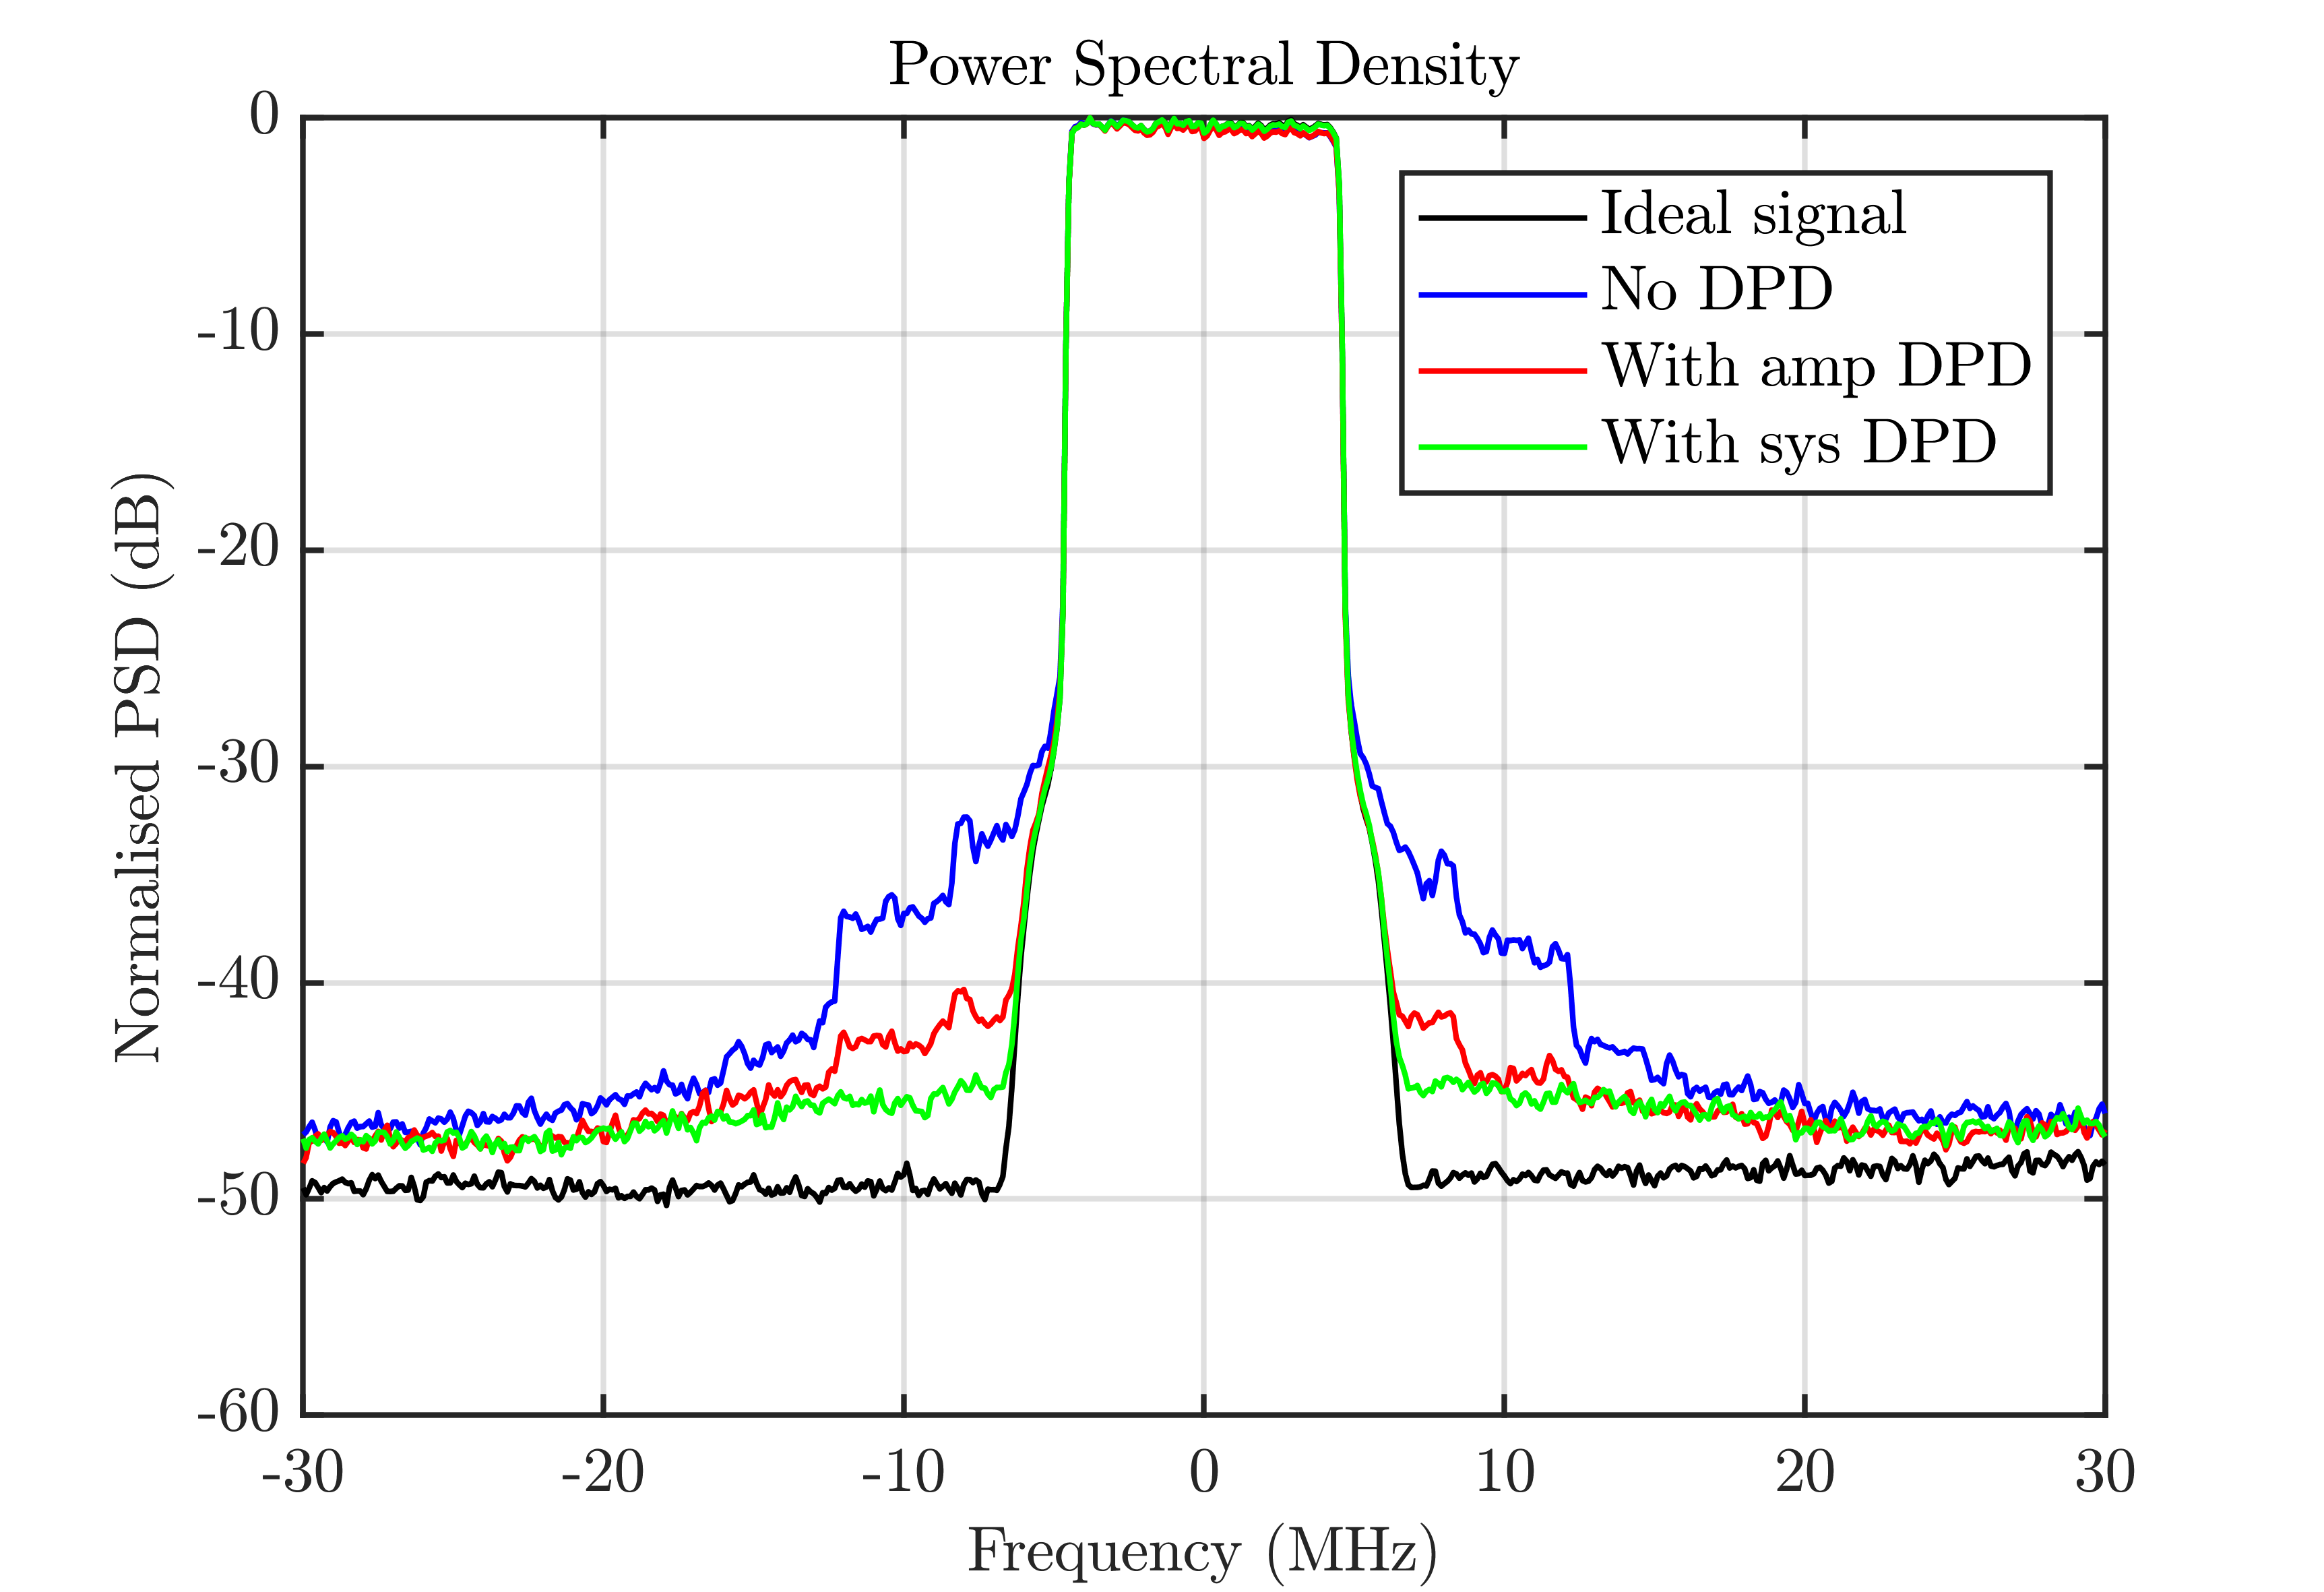
\includegraphics[scale = 0.5]{figures/measurement/cree/meas3/psd_0p2.png}
	\caption{PSD of measurement at $d = 0.2\lambda$}
    \label{fig:meas3_psd2}
  \end{minipage}
\end{figure}

\begin{figure}[H]
  \centering
  \begin{minipage}[b]{0.5\textwidth}
	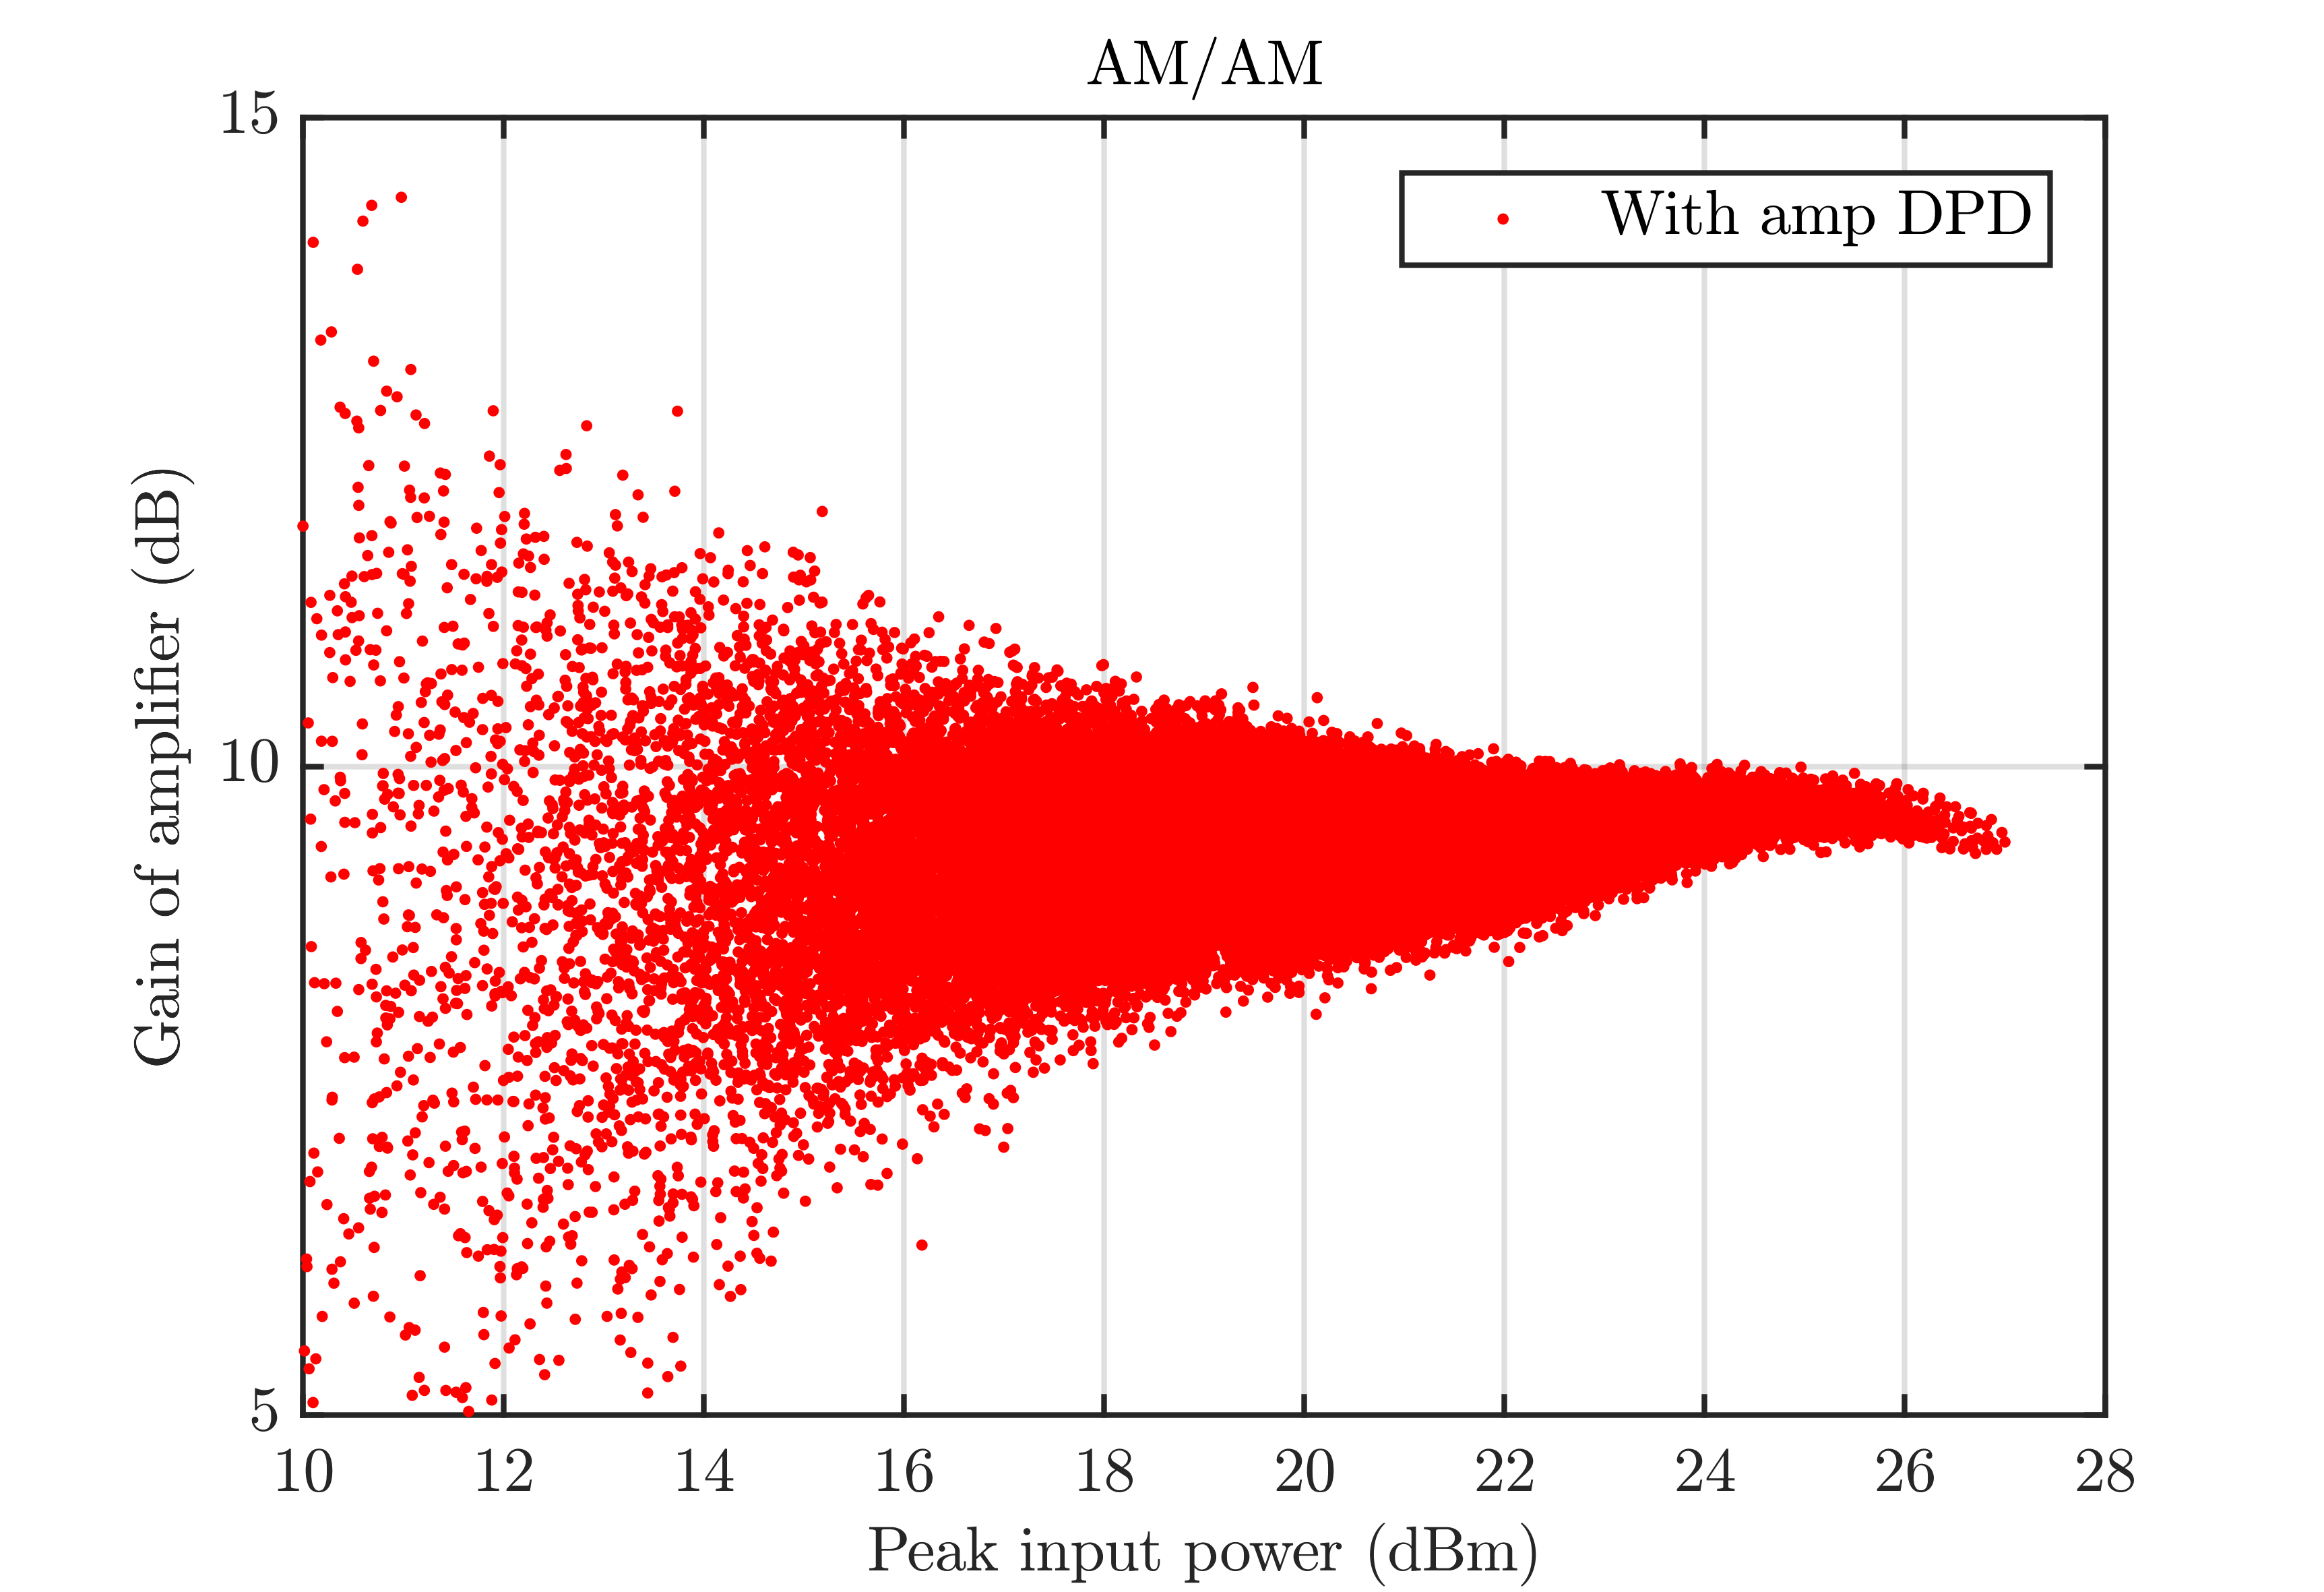
\includegraphics[scale = 0.5]{figures/measurement/cree/meas3/amam_amp_dpd_0p2.png}
	\caption{AM/AM distortion at $d = 0.2\lambda$ with amplifier DPD}	
    \label{fig:meas3_amam3}
  \end{minipage}
  \hfill
  \begin{minipage}[b]{0.4\textwidth}
	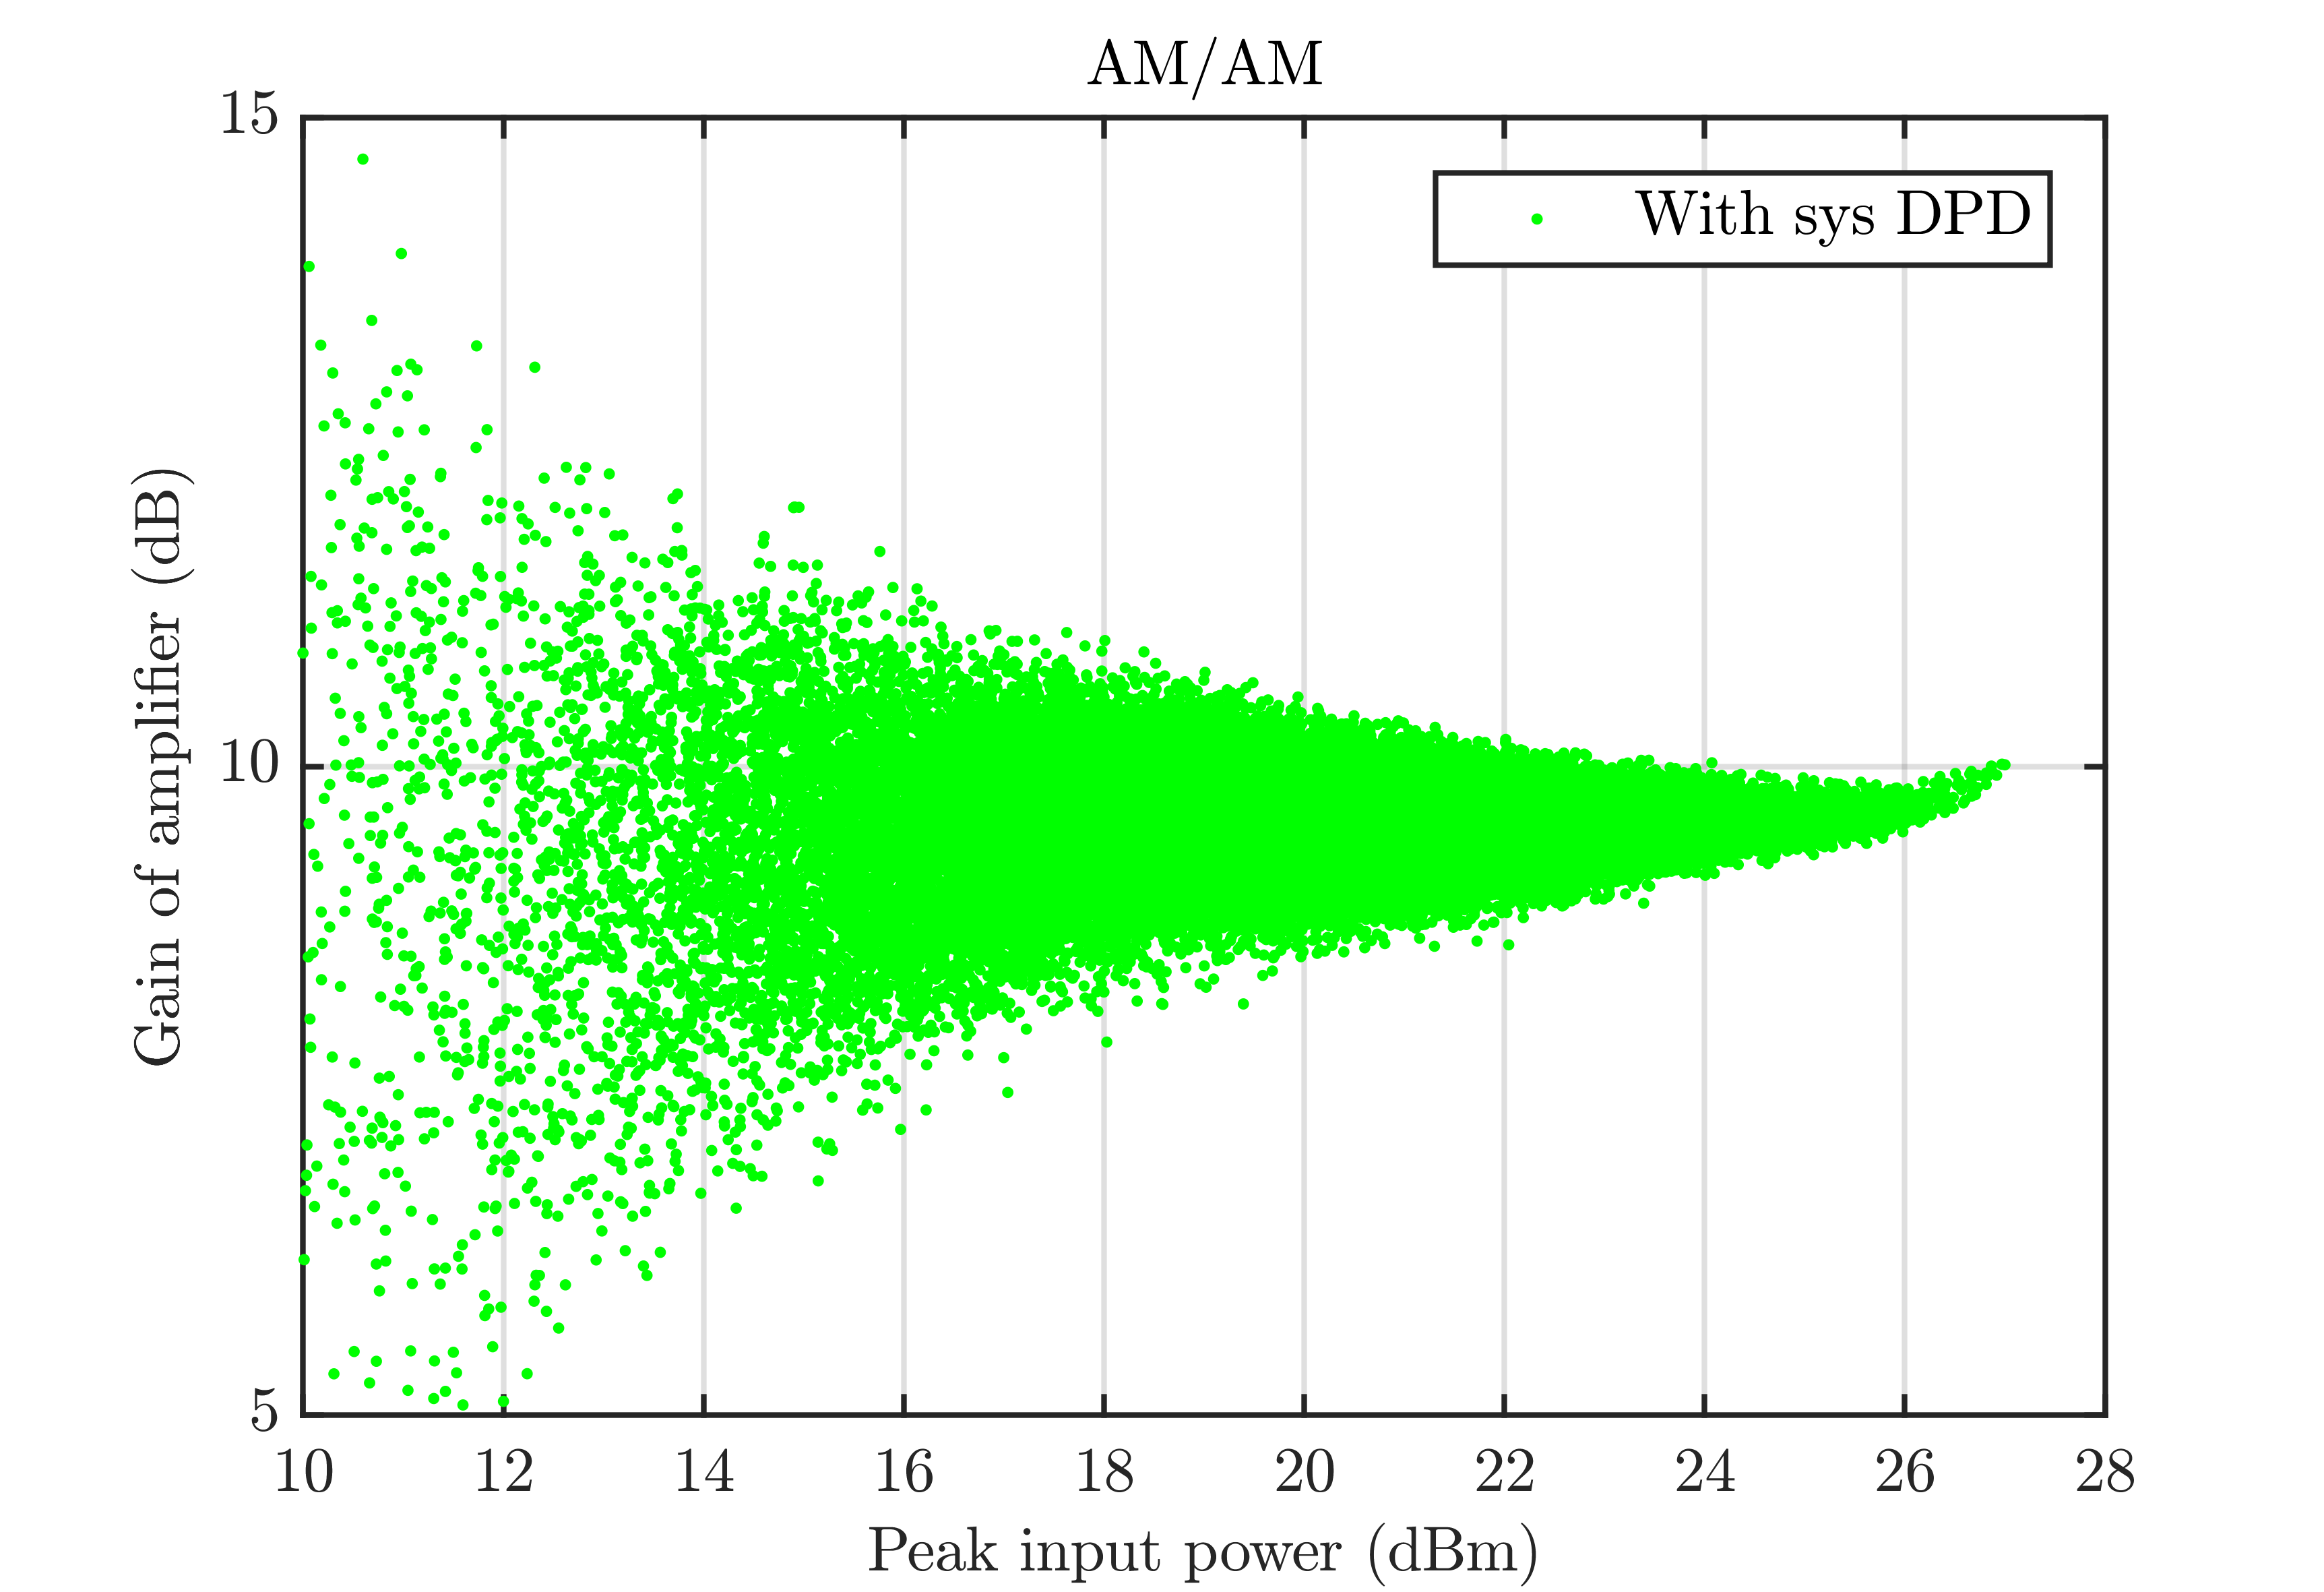
\includegraphics[scale = 0.5]{figures/measurement/cree/meas3/amam_sys_dpd_0p2.png}
	\caption{AM/AM distortion at $d = 0.2\lambda$ with system DPD}
    \label{fig:meas3_amam4}
  \end{minipage}
\end{figure}

\begin{figure}[H]
  \centering
  \begin{minipage}[b]{0.5\textwidth}
	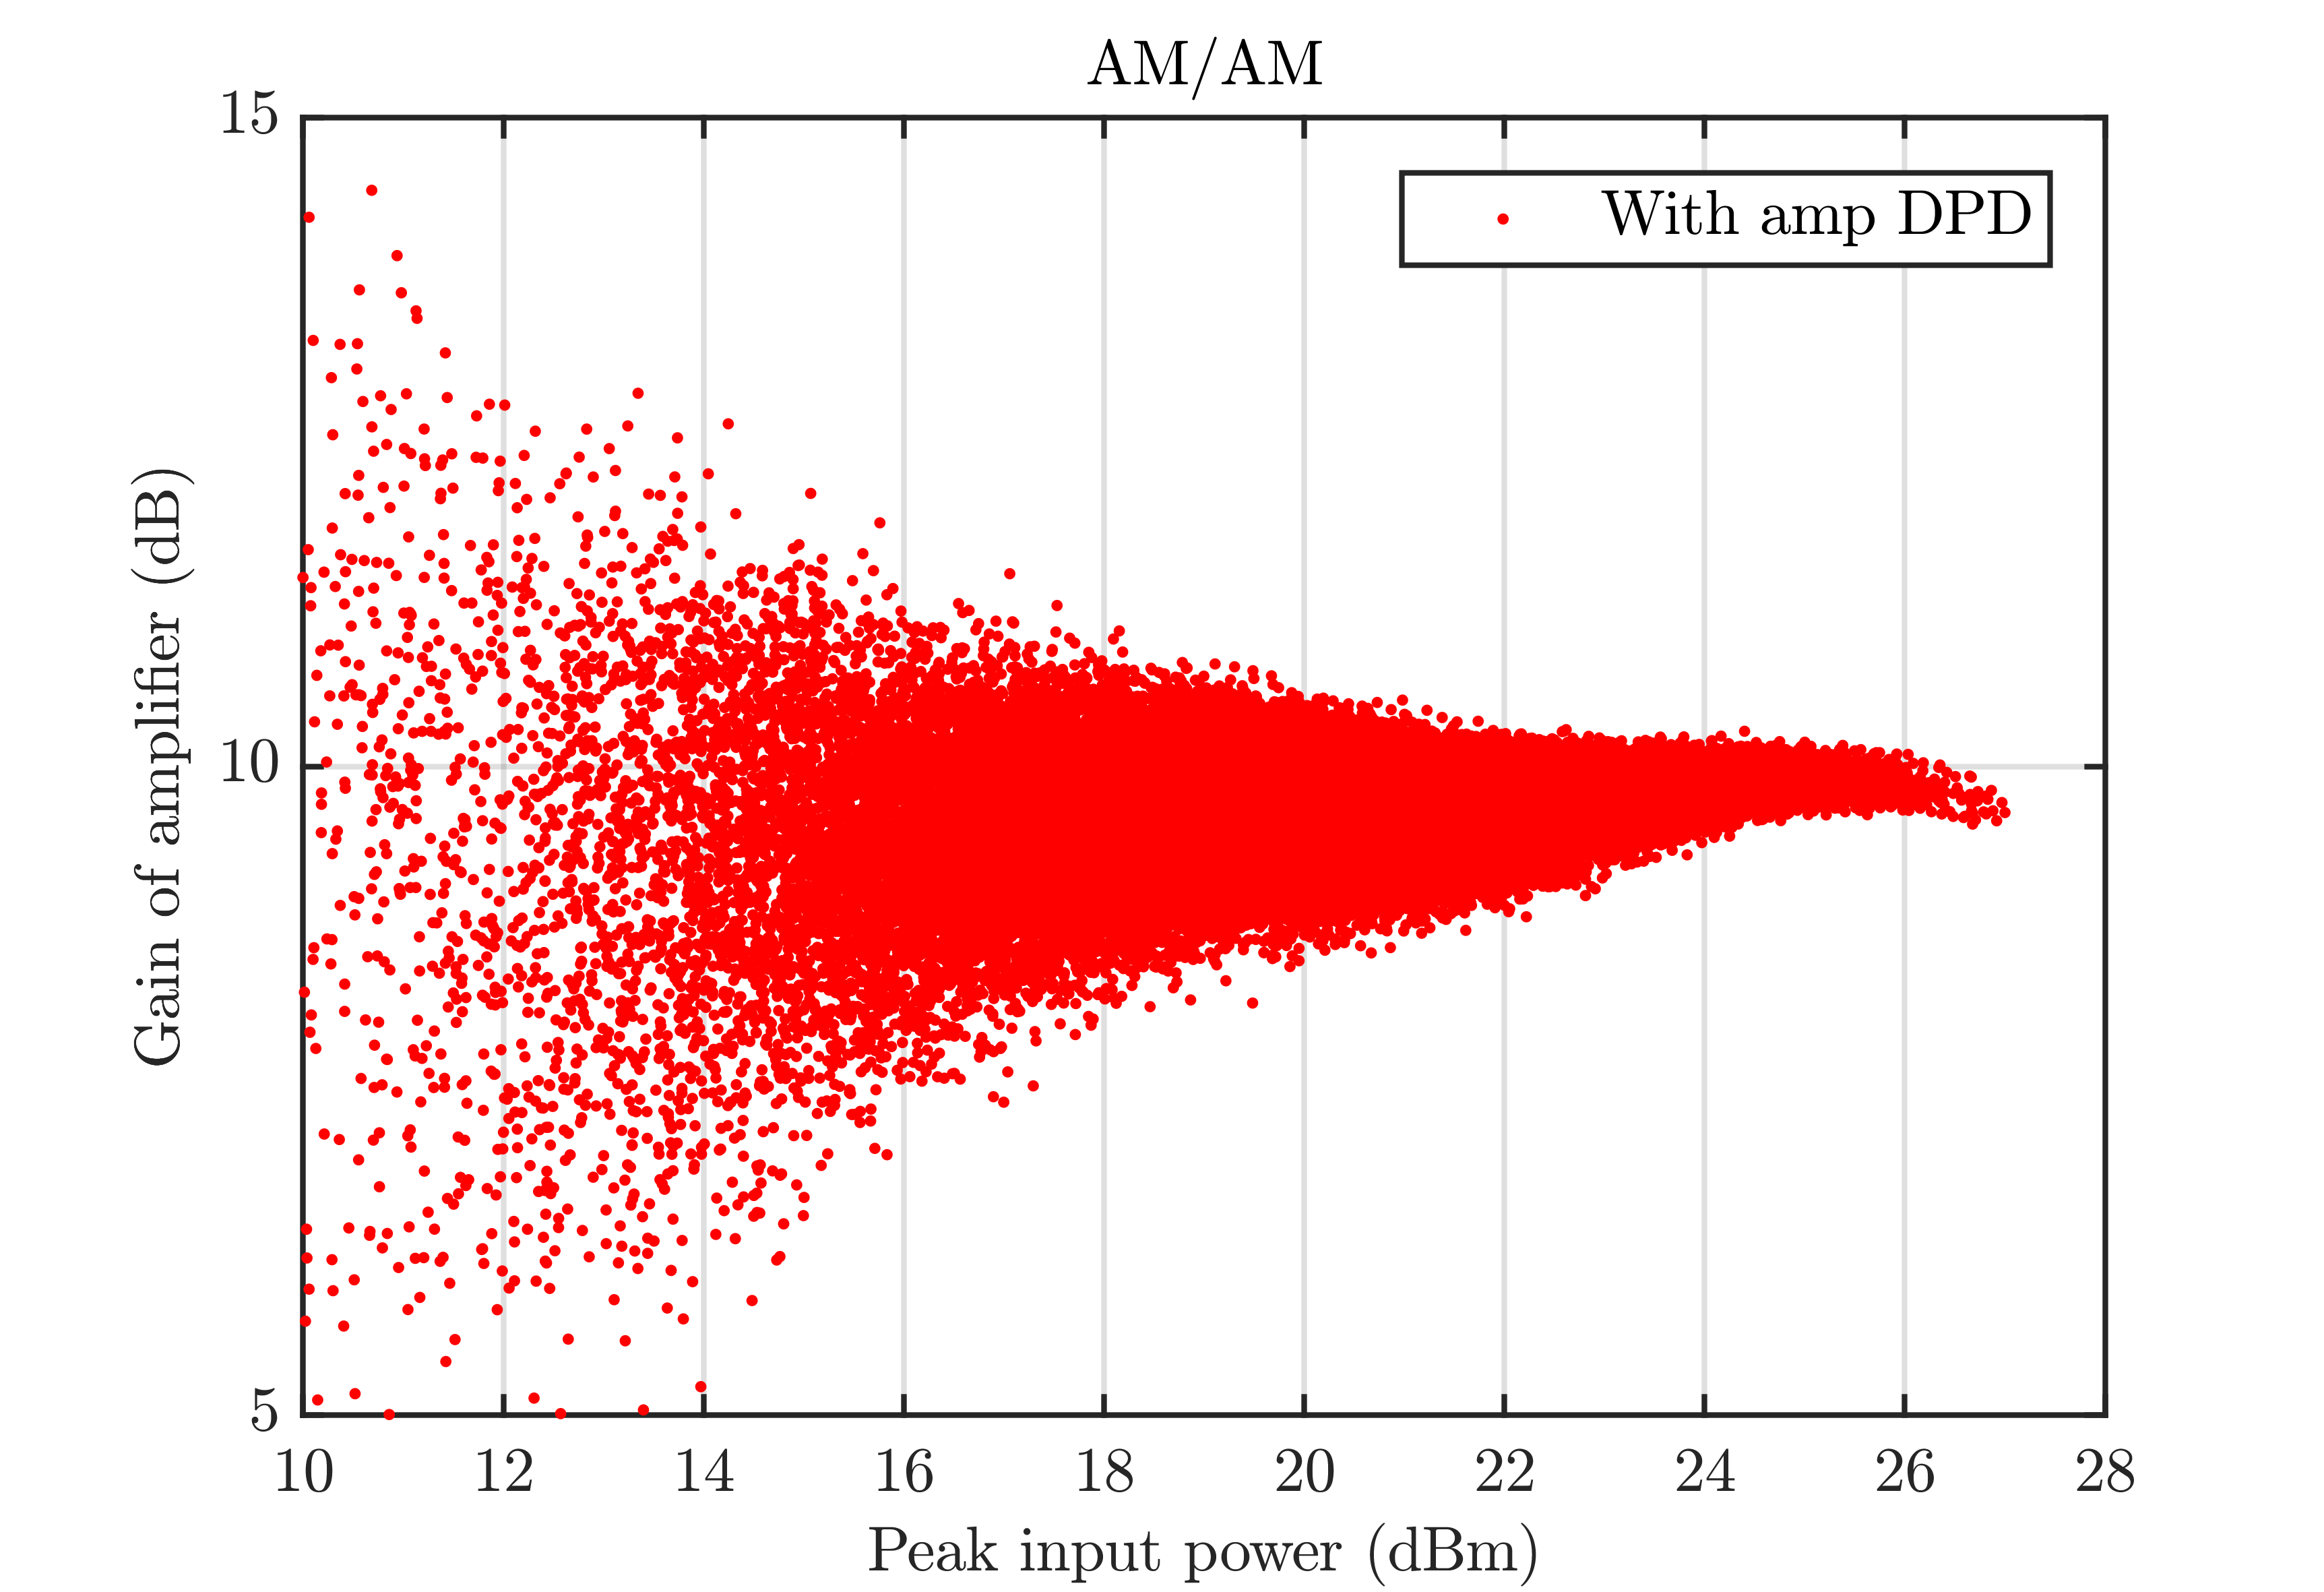
\includegraphics[scale = 0.5]{figures/measurement/cree/meas3/amam_amp_dpd_0p3.png}
	\caption{AM/AM distortion at $d = 0.3\lambda$ with amplifier DPD}	
    \label{fig:meas3_amam5}
  \end{minipage}
  \hfill
  \begin{minipage}[b]{0.4\textwidth}
	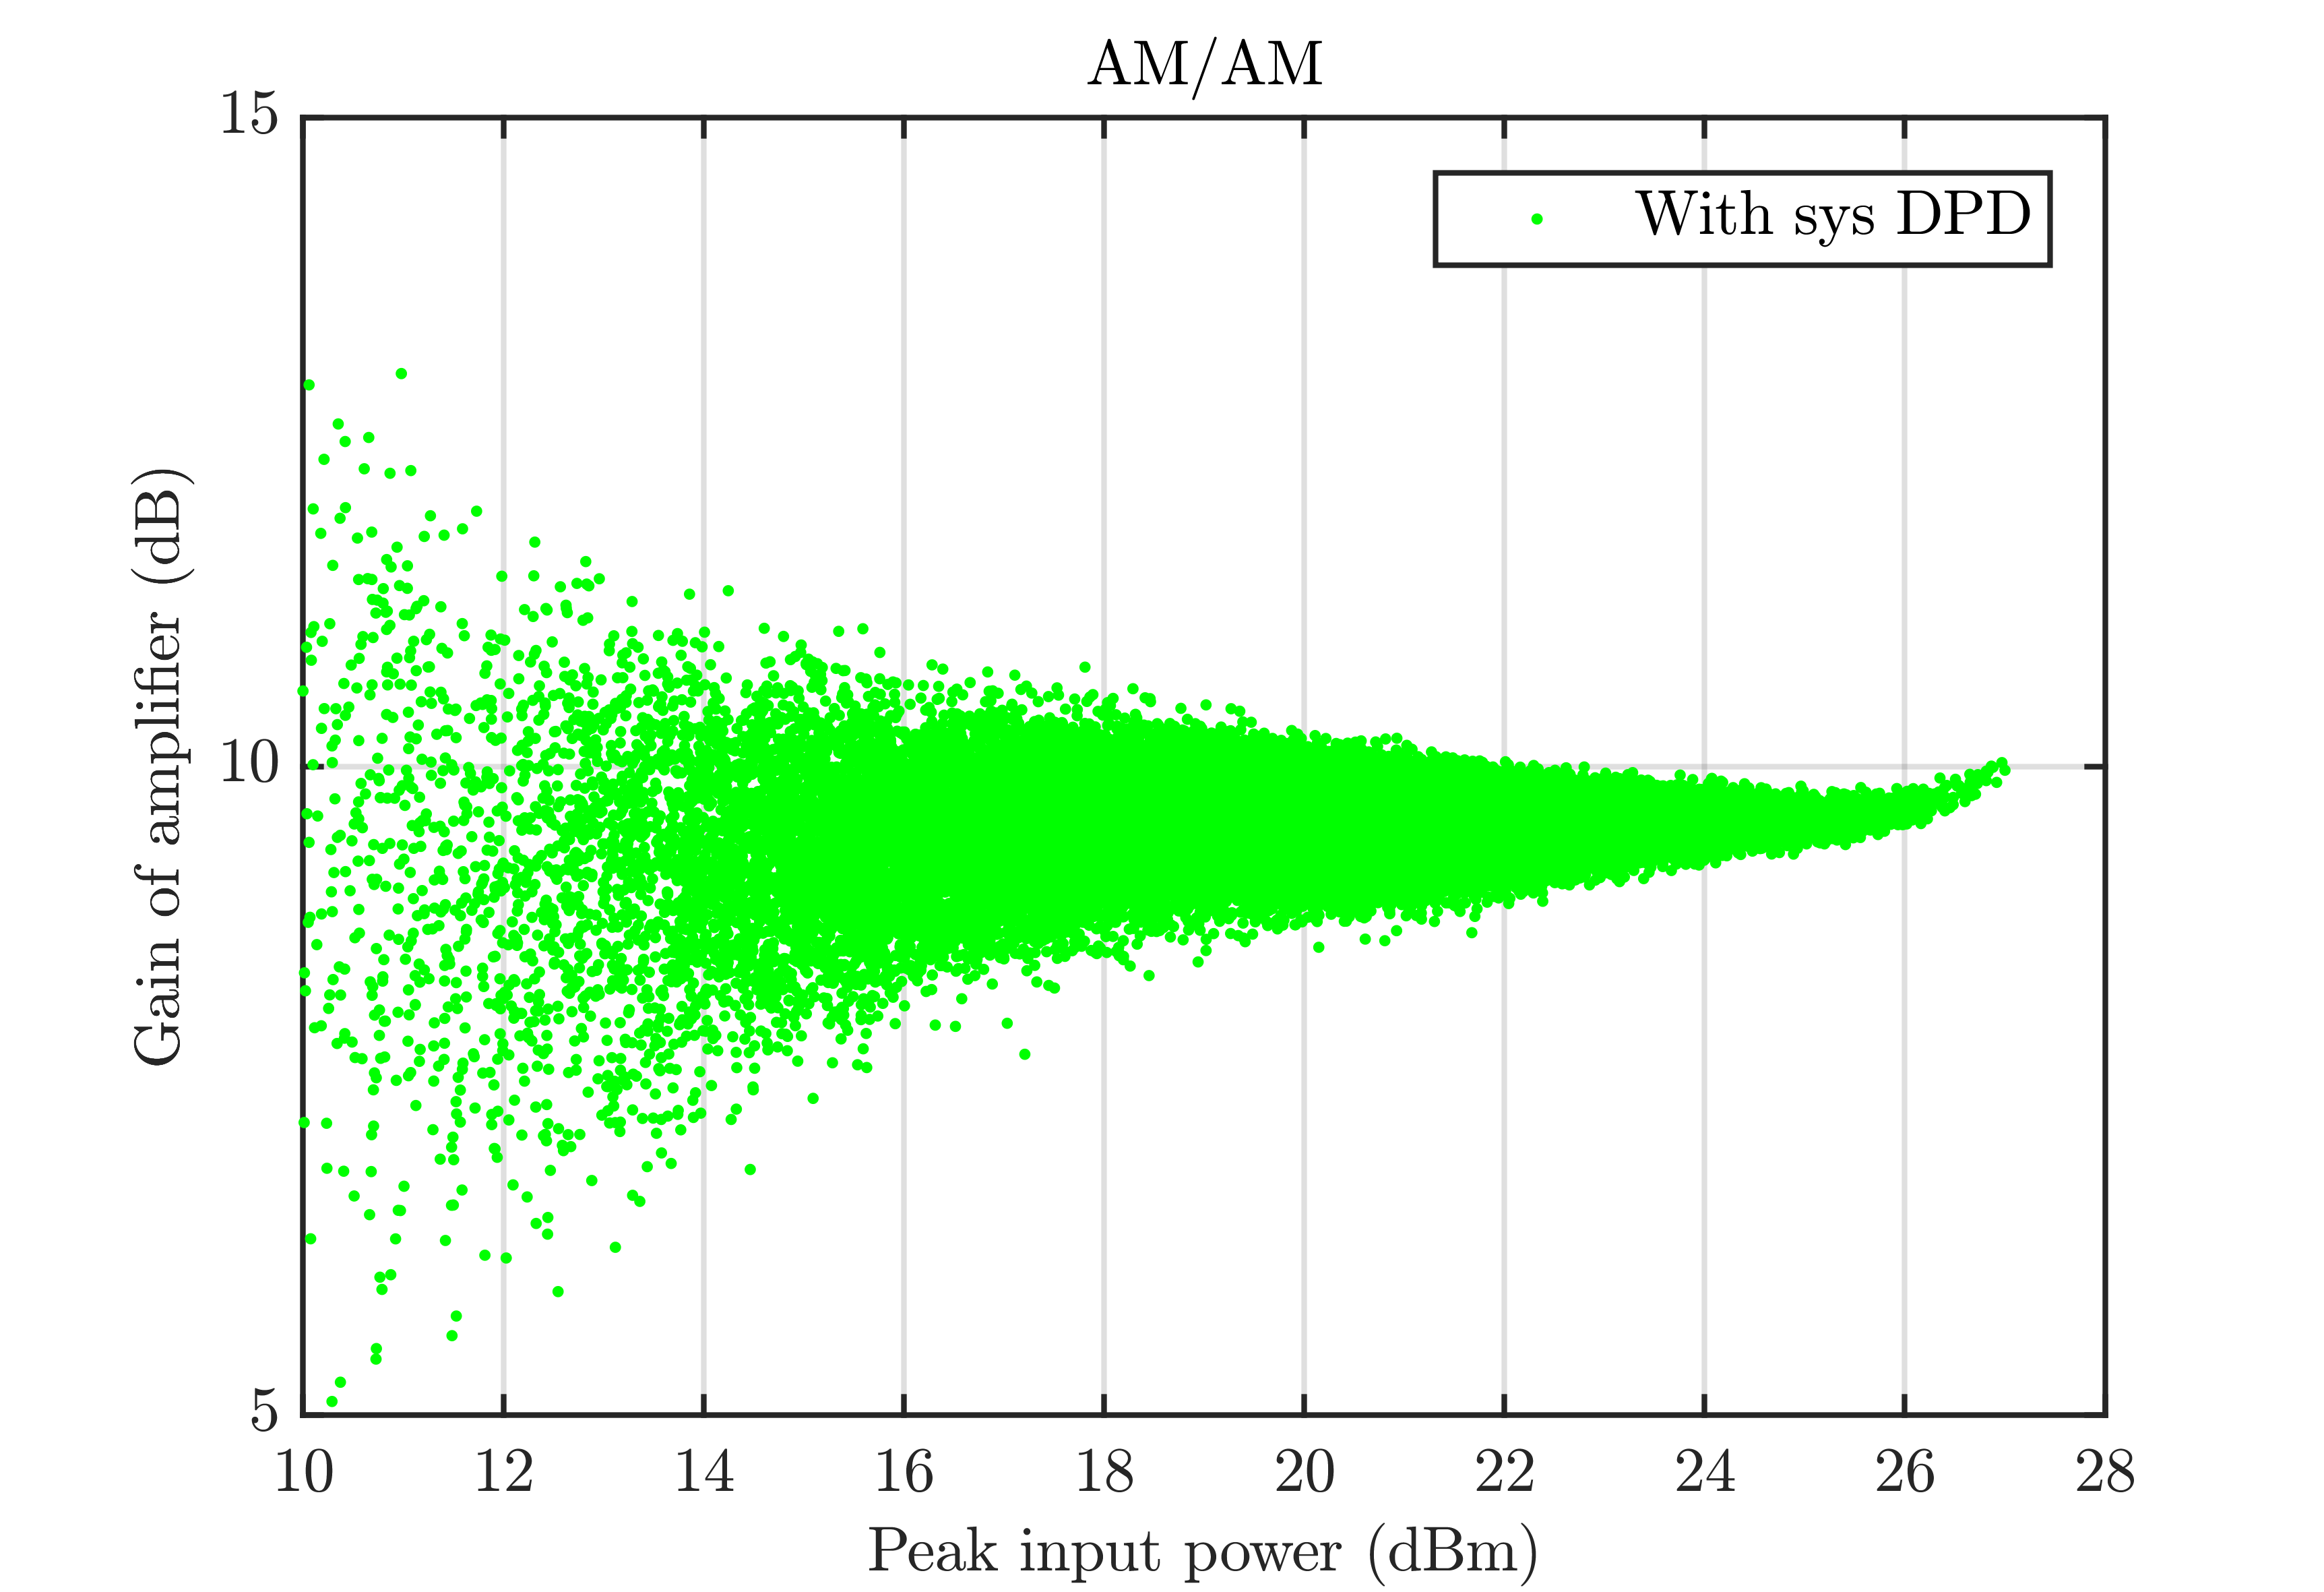
\includegraphics[scale = 0.5]{figures/measurement/cree/meas3/amam_sys_dpd_0p3.png}
	\caption{AM/AM distortion at $d = 0.3\lambda$ with system DPD}
    \label{fig:meas3_amam6}
  \end{minipage}
\end{figure}

\begin{figure}[H]
  \centering
  \begin{minipage}[b]{0.5\textwidth}
	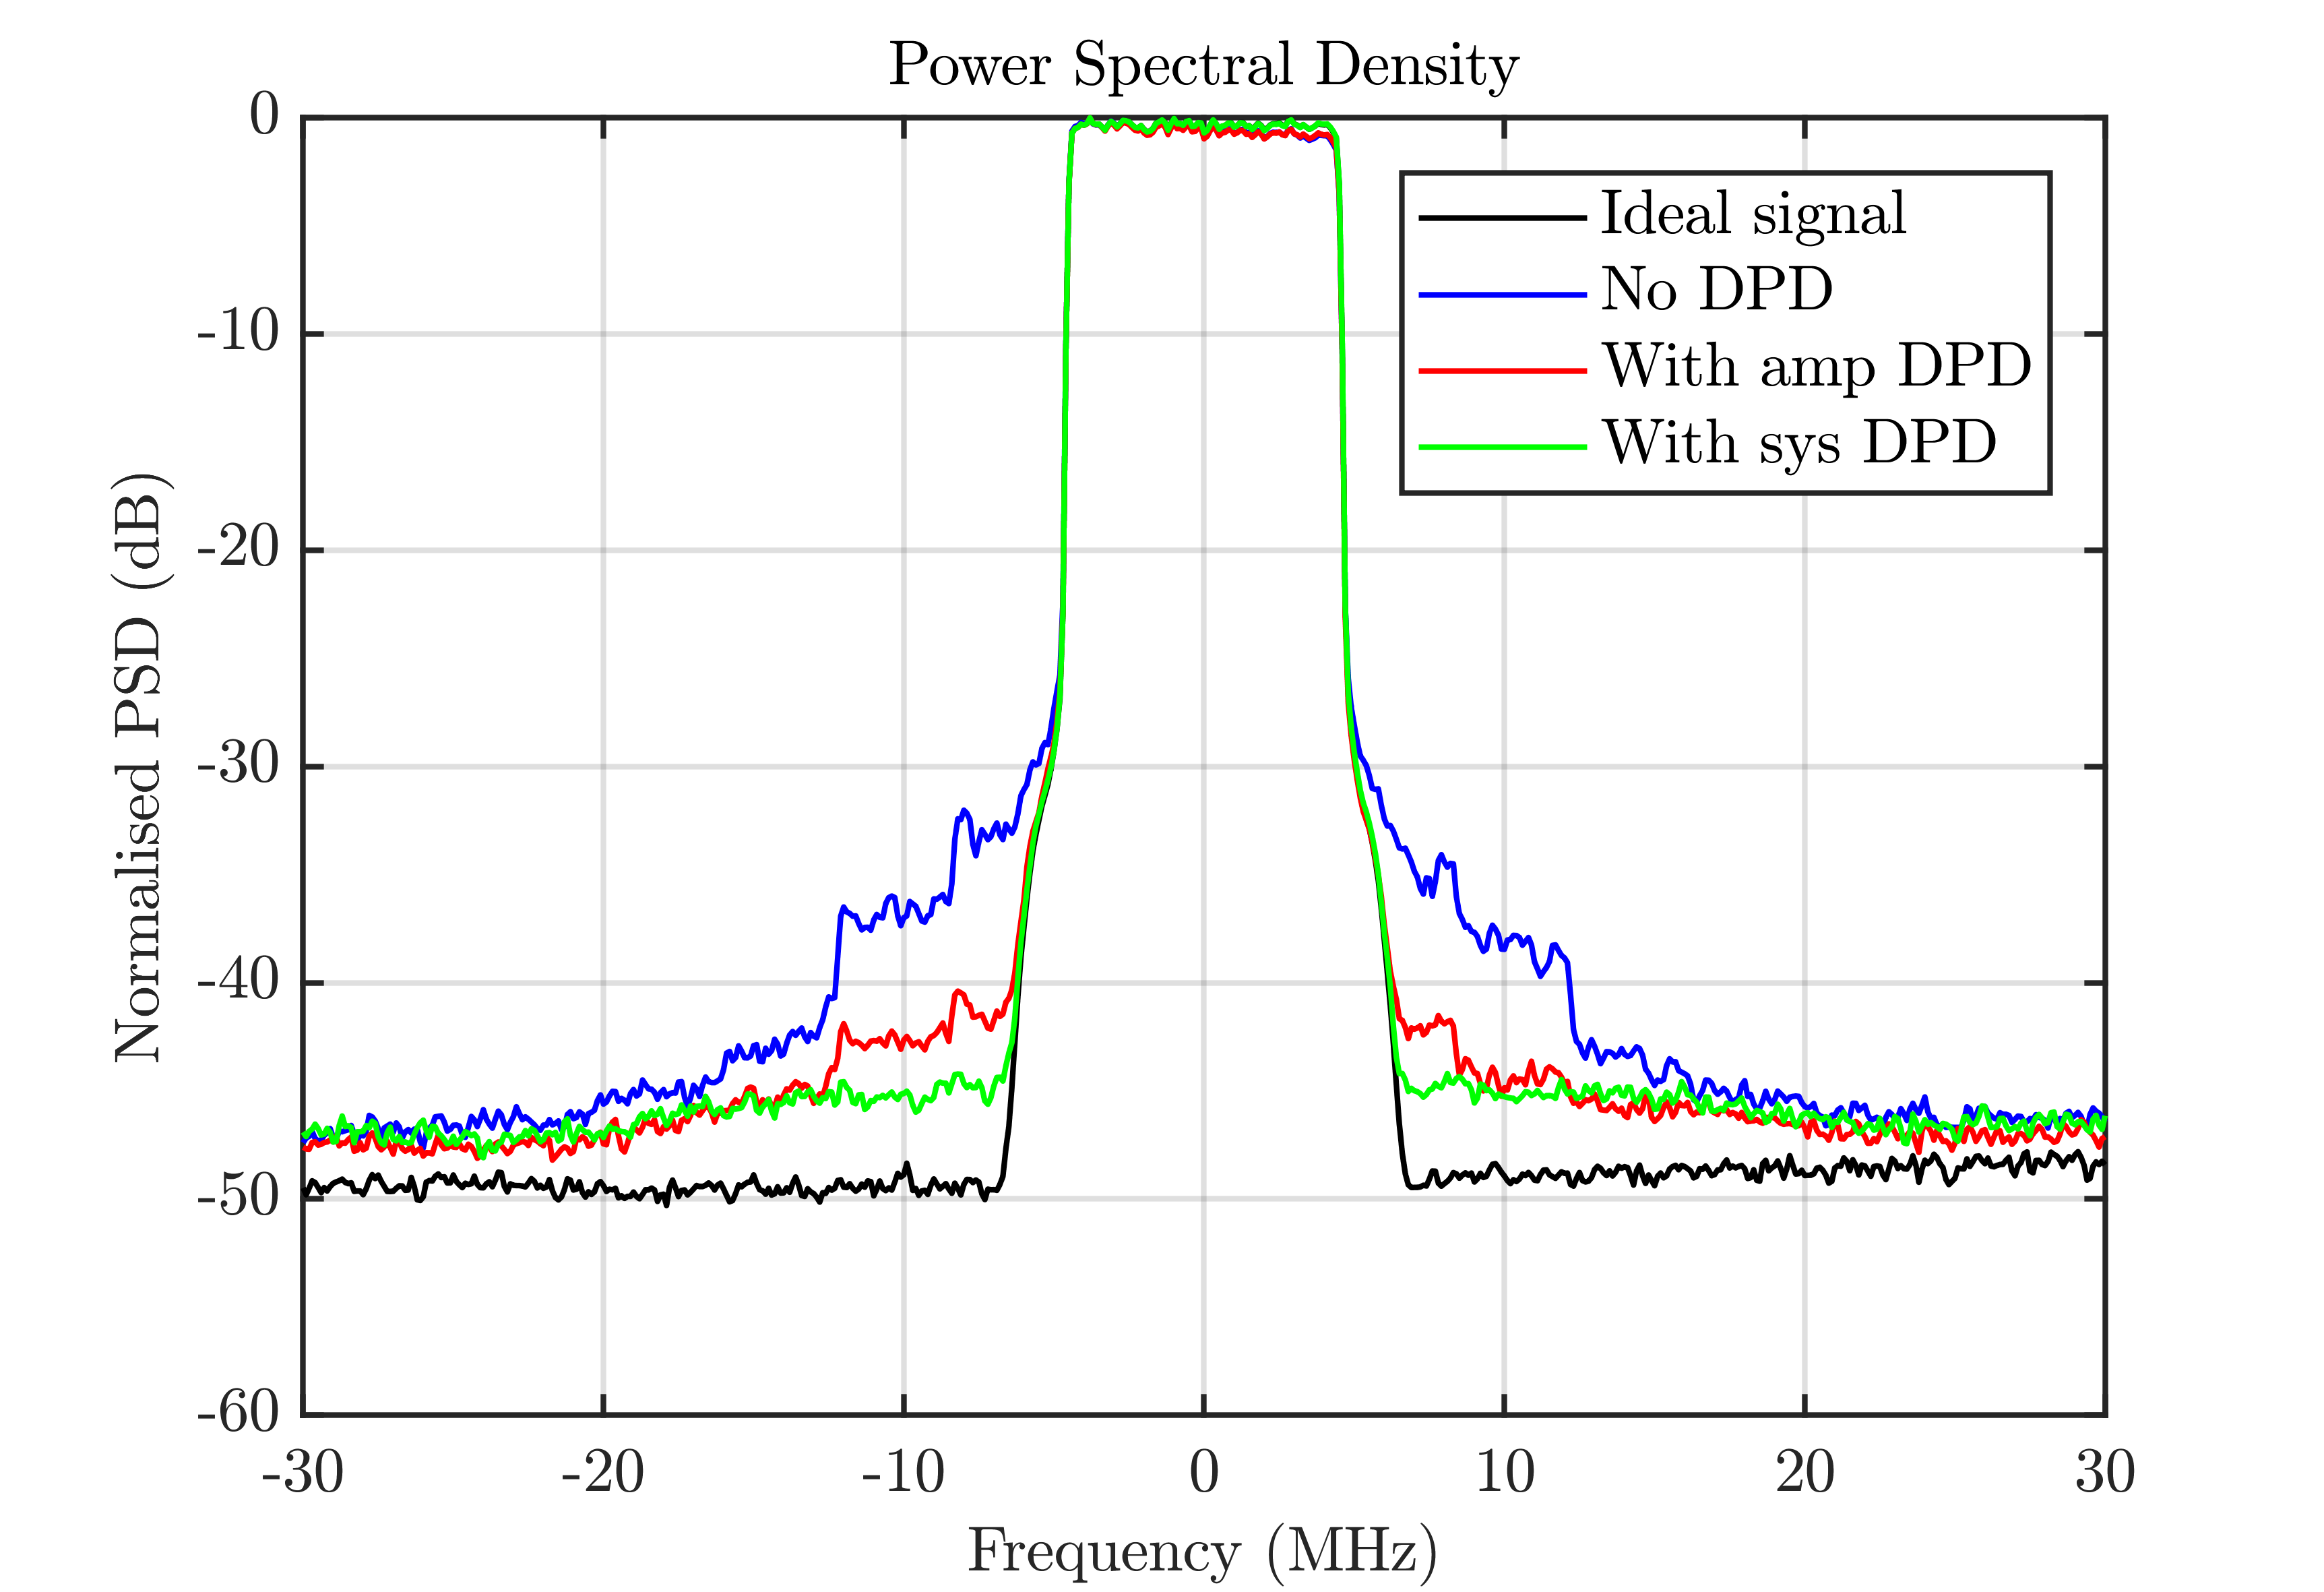
\includegraphics[scale = 0.5]{figures/measurement/cree/meas3/psd_0p3.png}
	\caption{PSD of measurement at $d = 0.3\lambda$ }	
    \label{fig:meas3_psd3}
  \end{minipage}
  \hfill
  \begin{minipage}[b]{0.4\textwidth}
	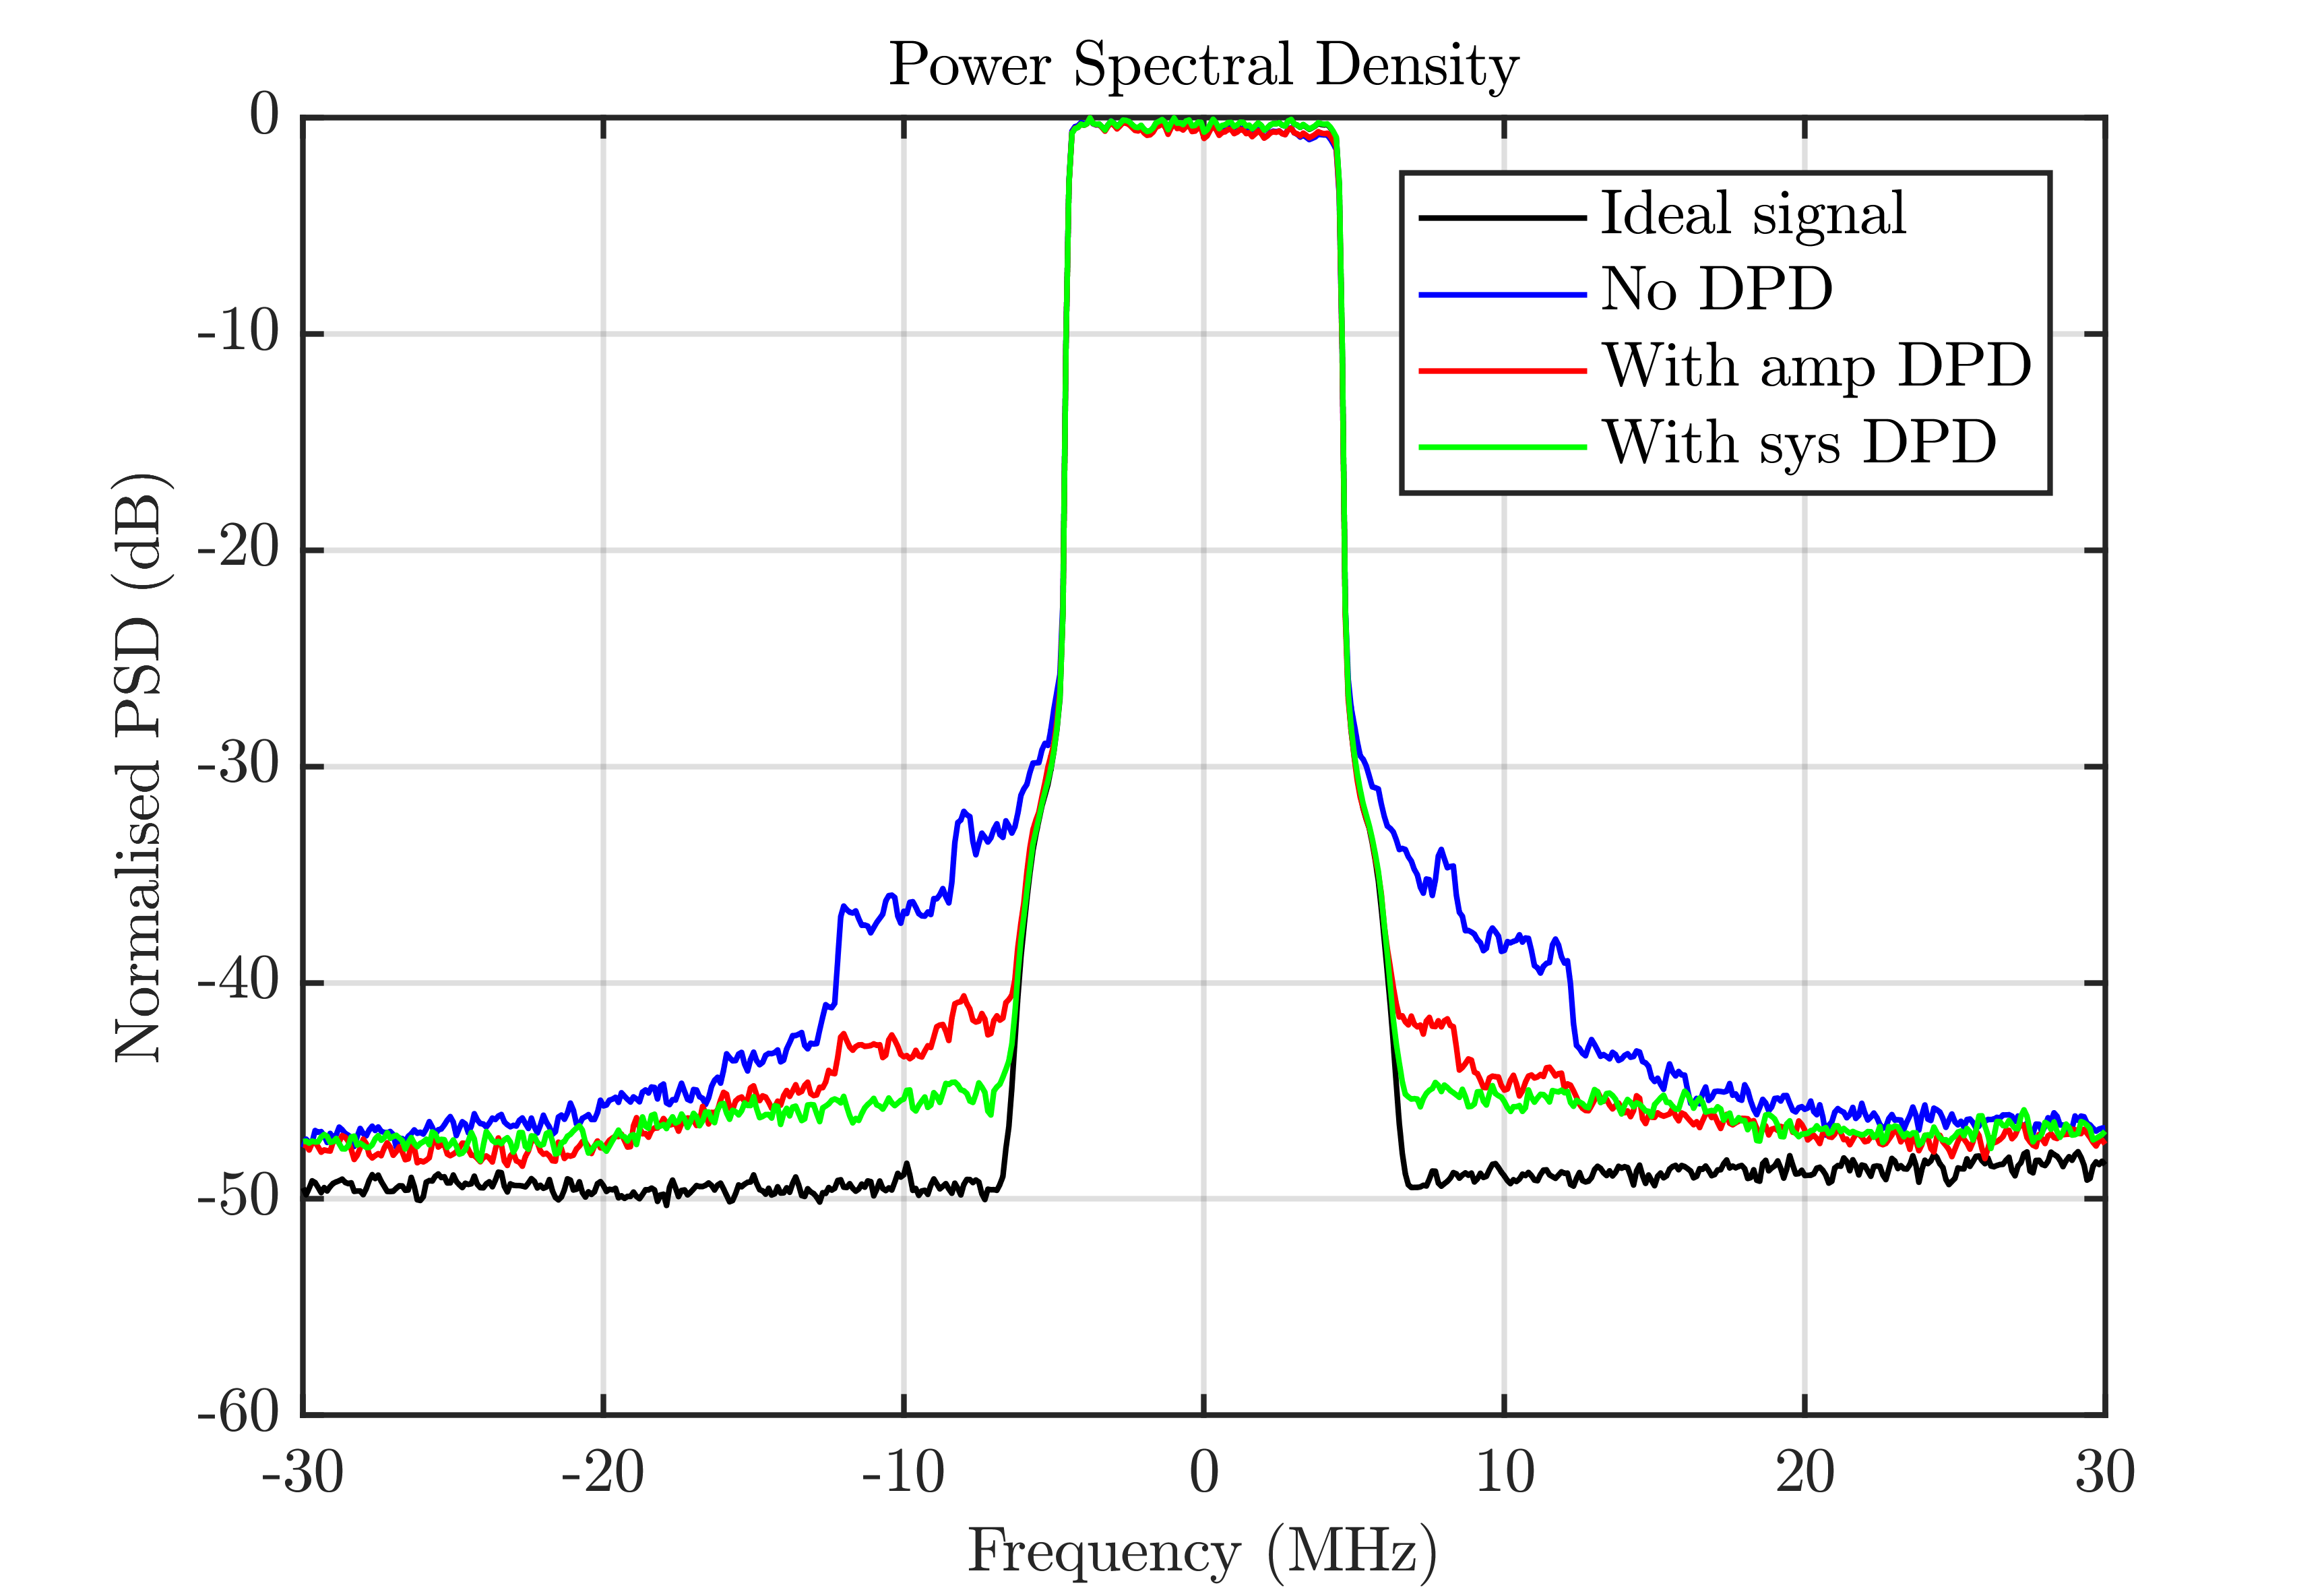
\includegraphics[scale = 0.5]{figures/measurement/cree/meas3/psd_0p4.png}
	\caption{PSD of measurement at $d = 0.4\lambda$}
    \label{fig:meas3_psd4}
  \end{minipage}
\end{figure}

\begin{figure}[H]
  \centering
  \begin{minipage}[b]{0.5\textwidth}
	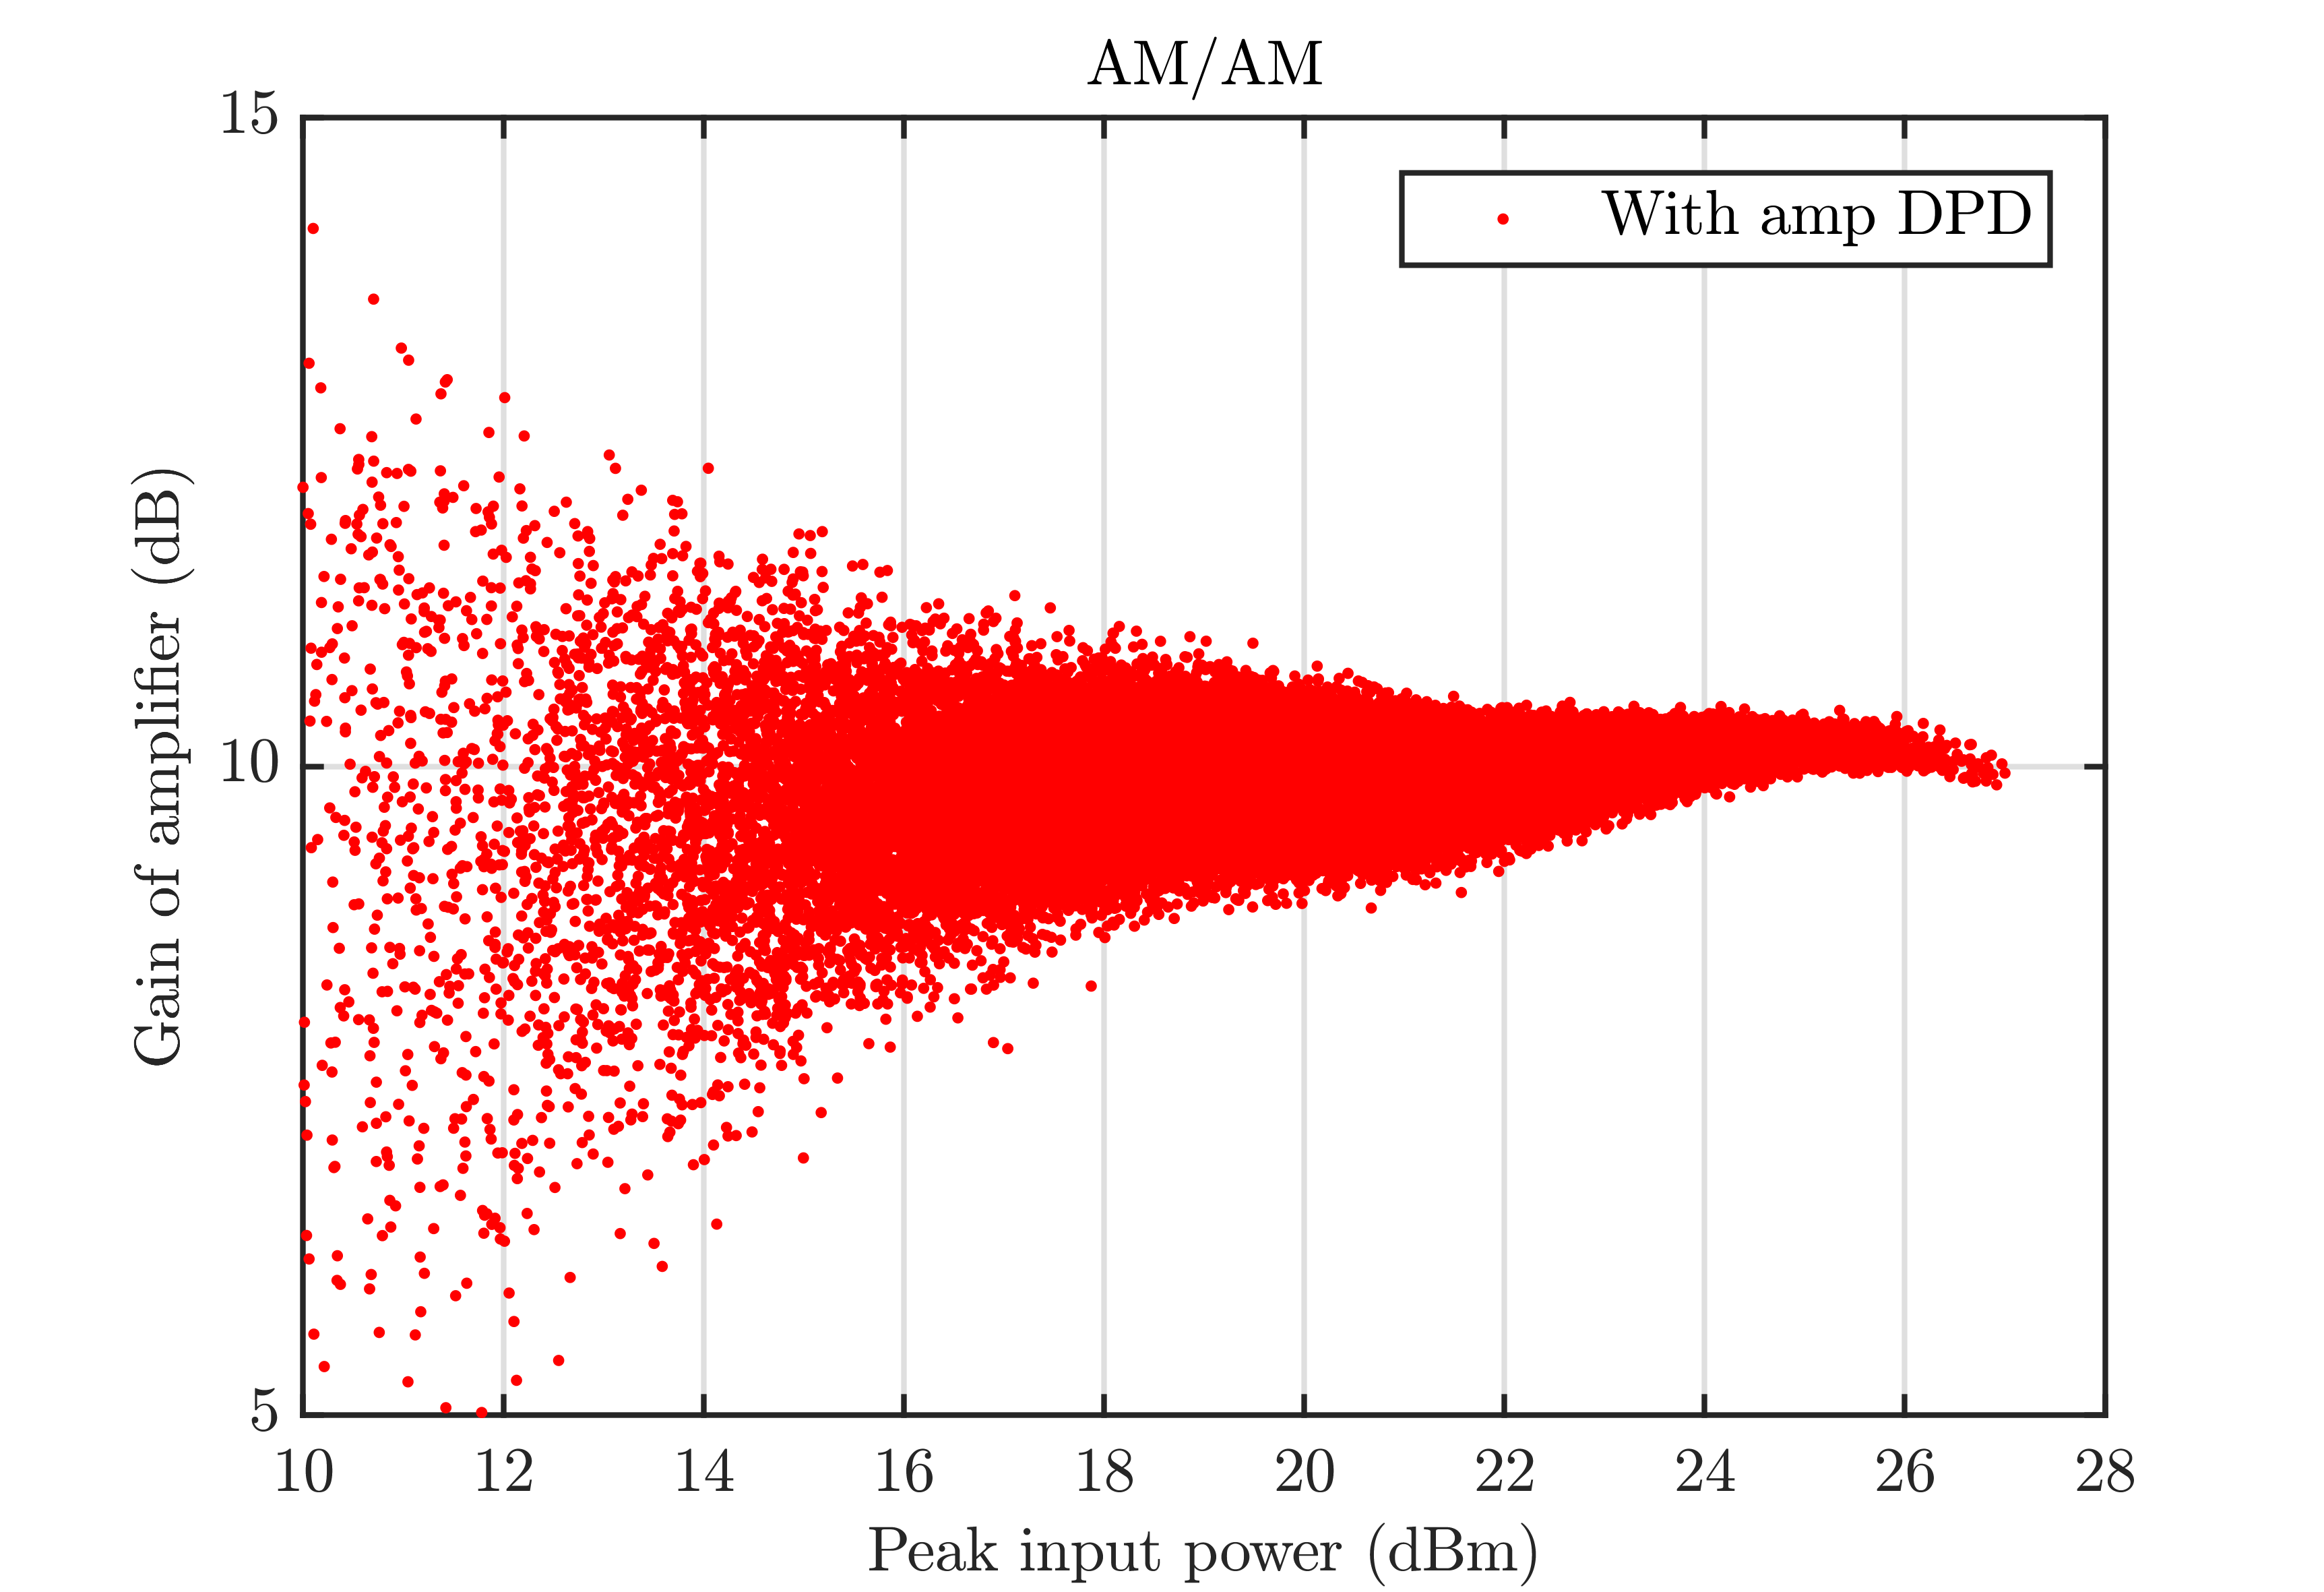
\includegraphics[scale = 0.5]{figures/measurement/cree/meas3/amam_amp_dpd_0p4.png}
	\caption{AM/AM distortion at $d = 0.4\lambda$ with amplifier DPD}	
    \label{fig:meas3_amam7}
  \end{minipage}
  \hfill
  \begin{minipage}[b]{0.4\textwidth}
	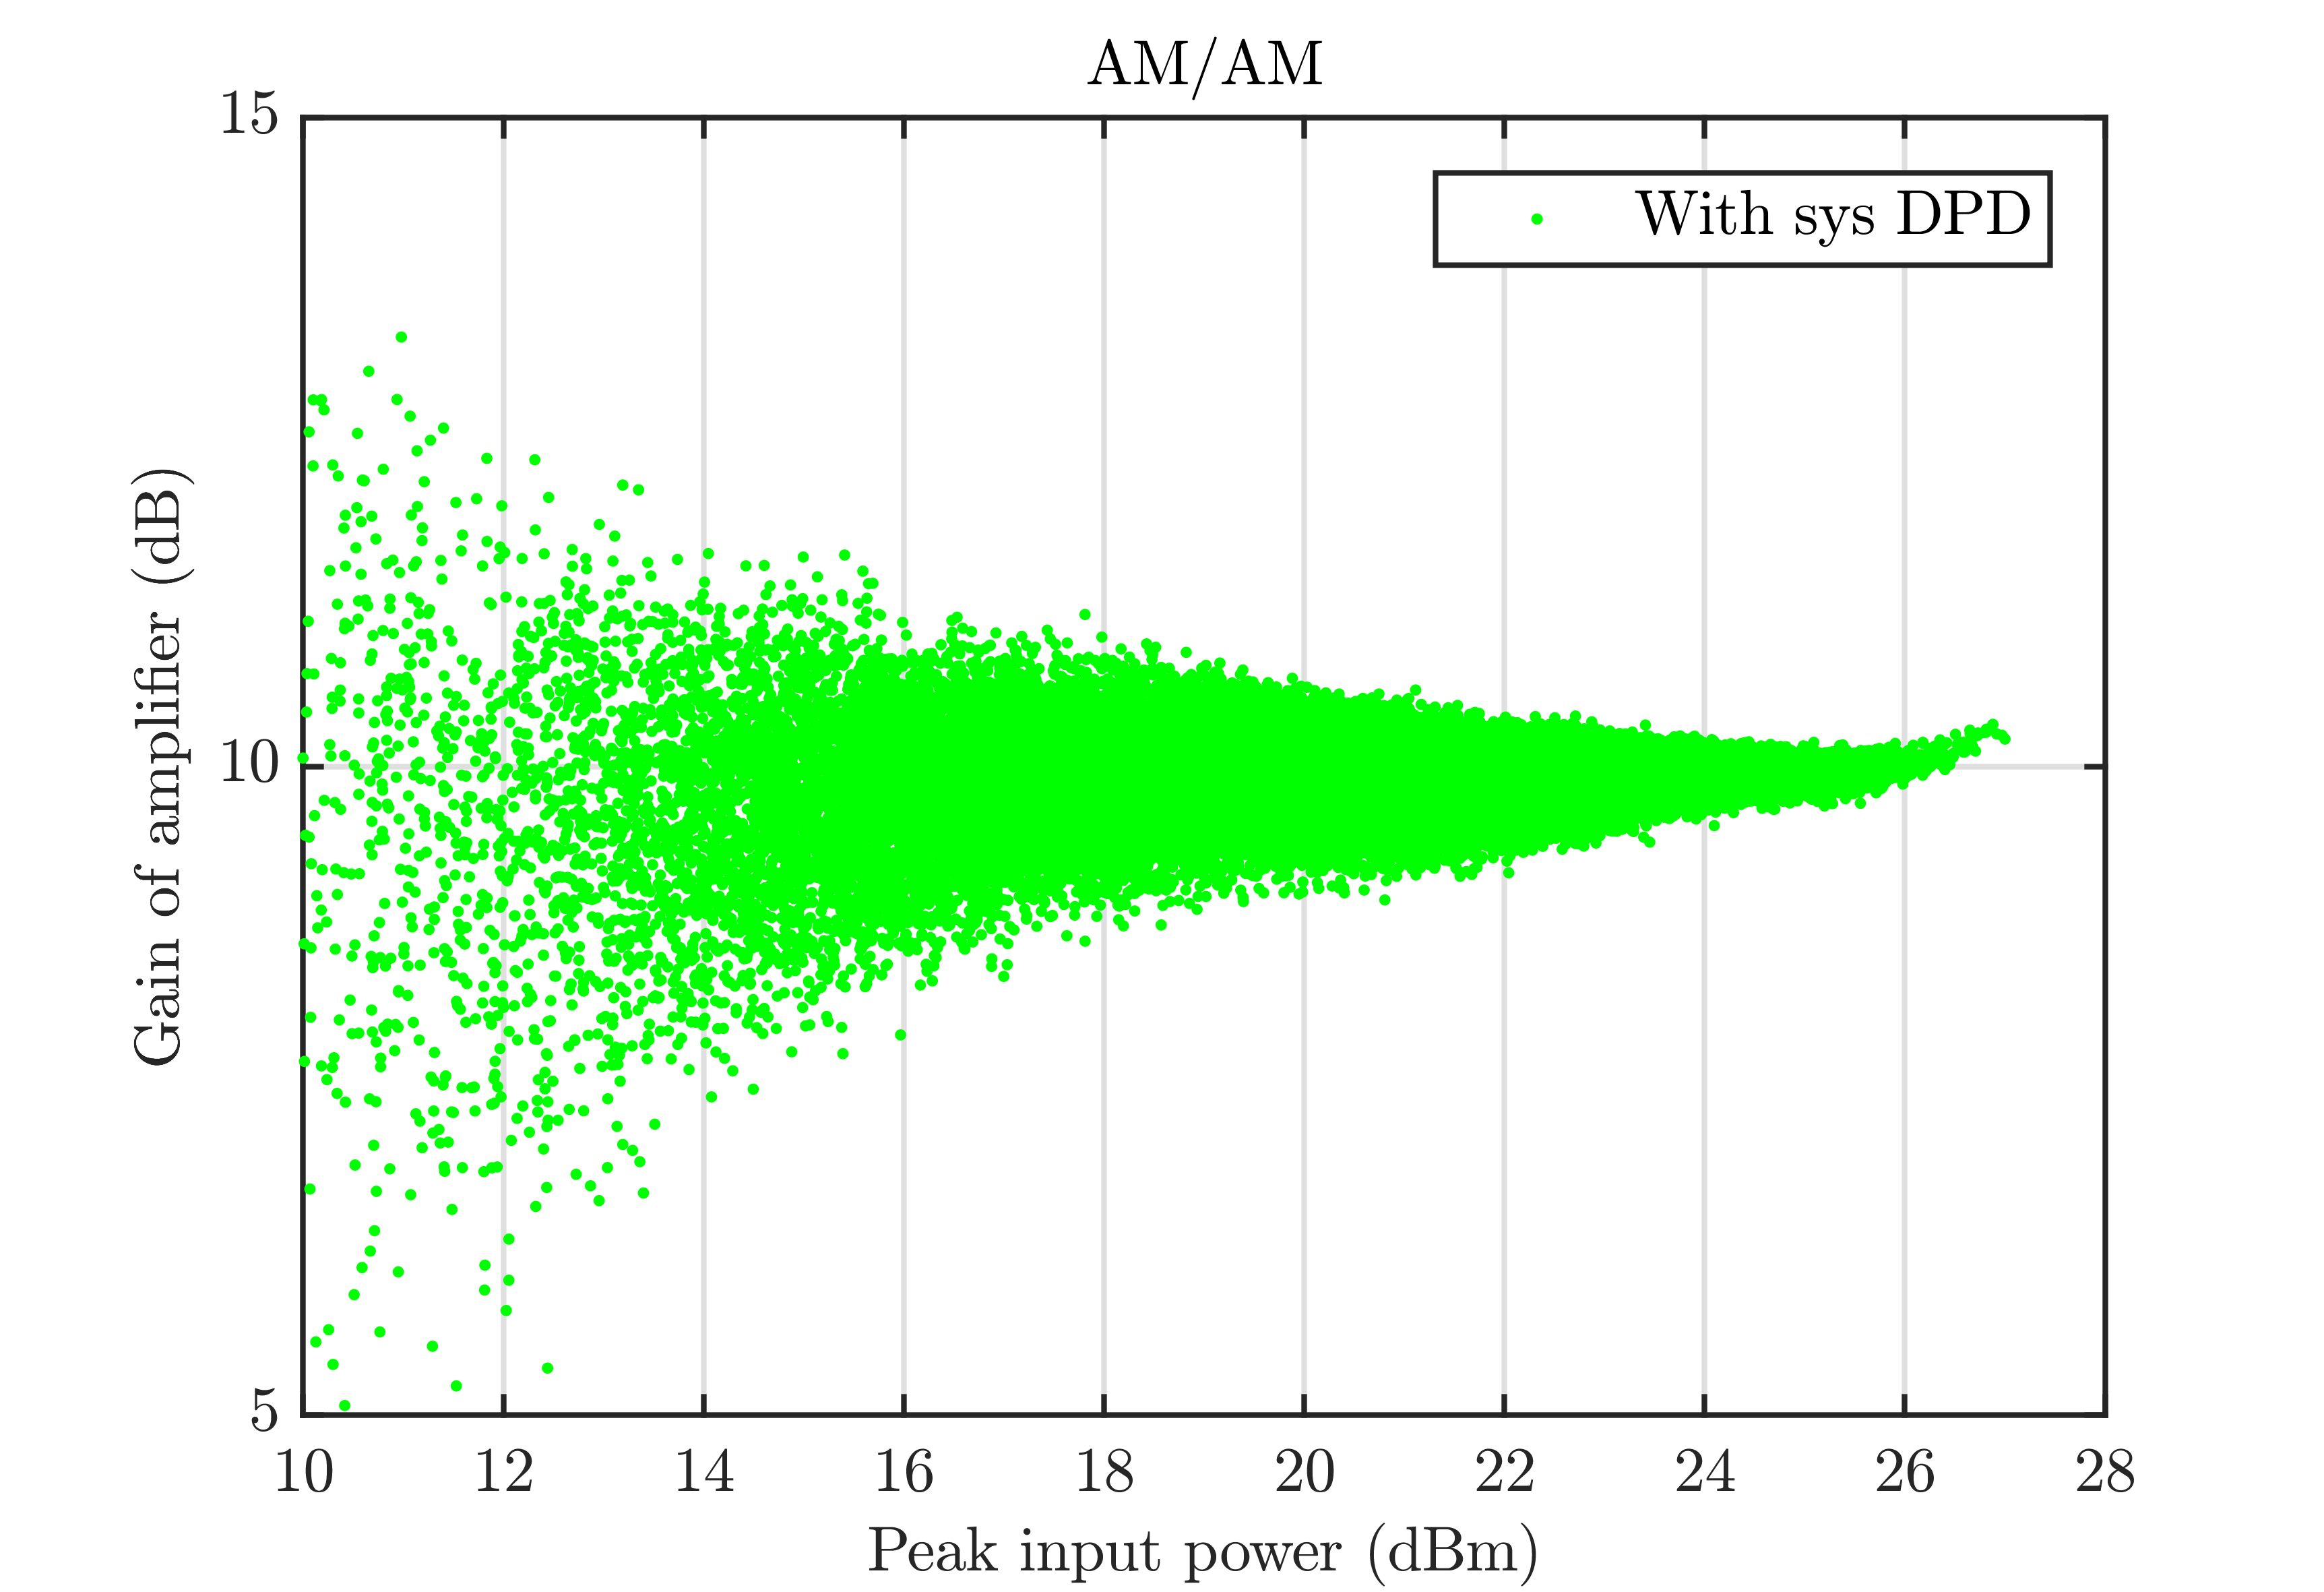
\includegraphics[scale = 0.5]{figures/measurement/cree/meas3/amam_sys_dpd_0p4.png}
	\caption{AM/AM distortion at $d = 0.4\lambda$ with system DPD}
    \label{fig:meas3_amam8}
  \end{minipage}
\end{figure}

\begin{figure}[H]
  \centering
  \begin{minipage}[b]{0.5\textwidth}
	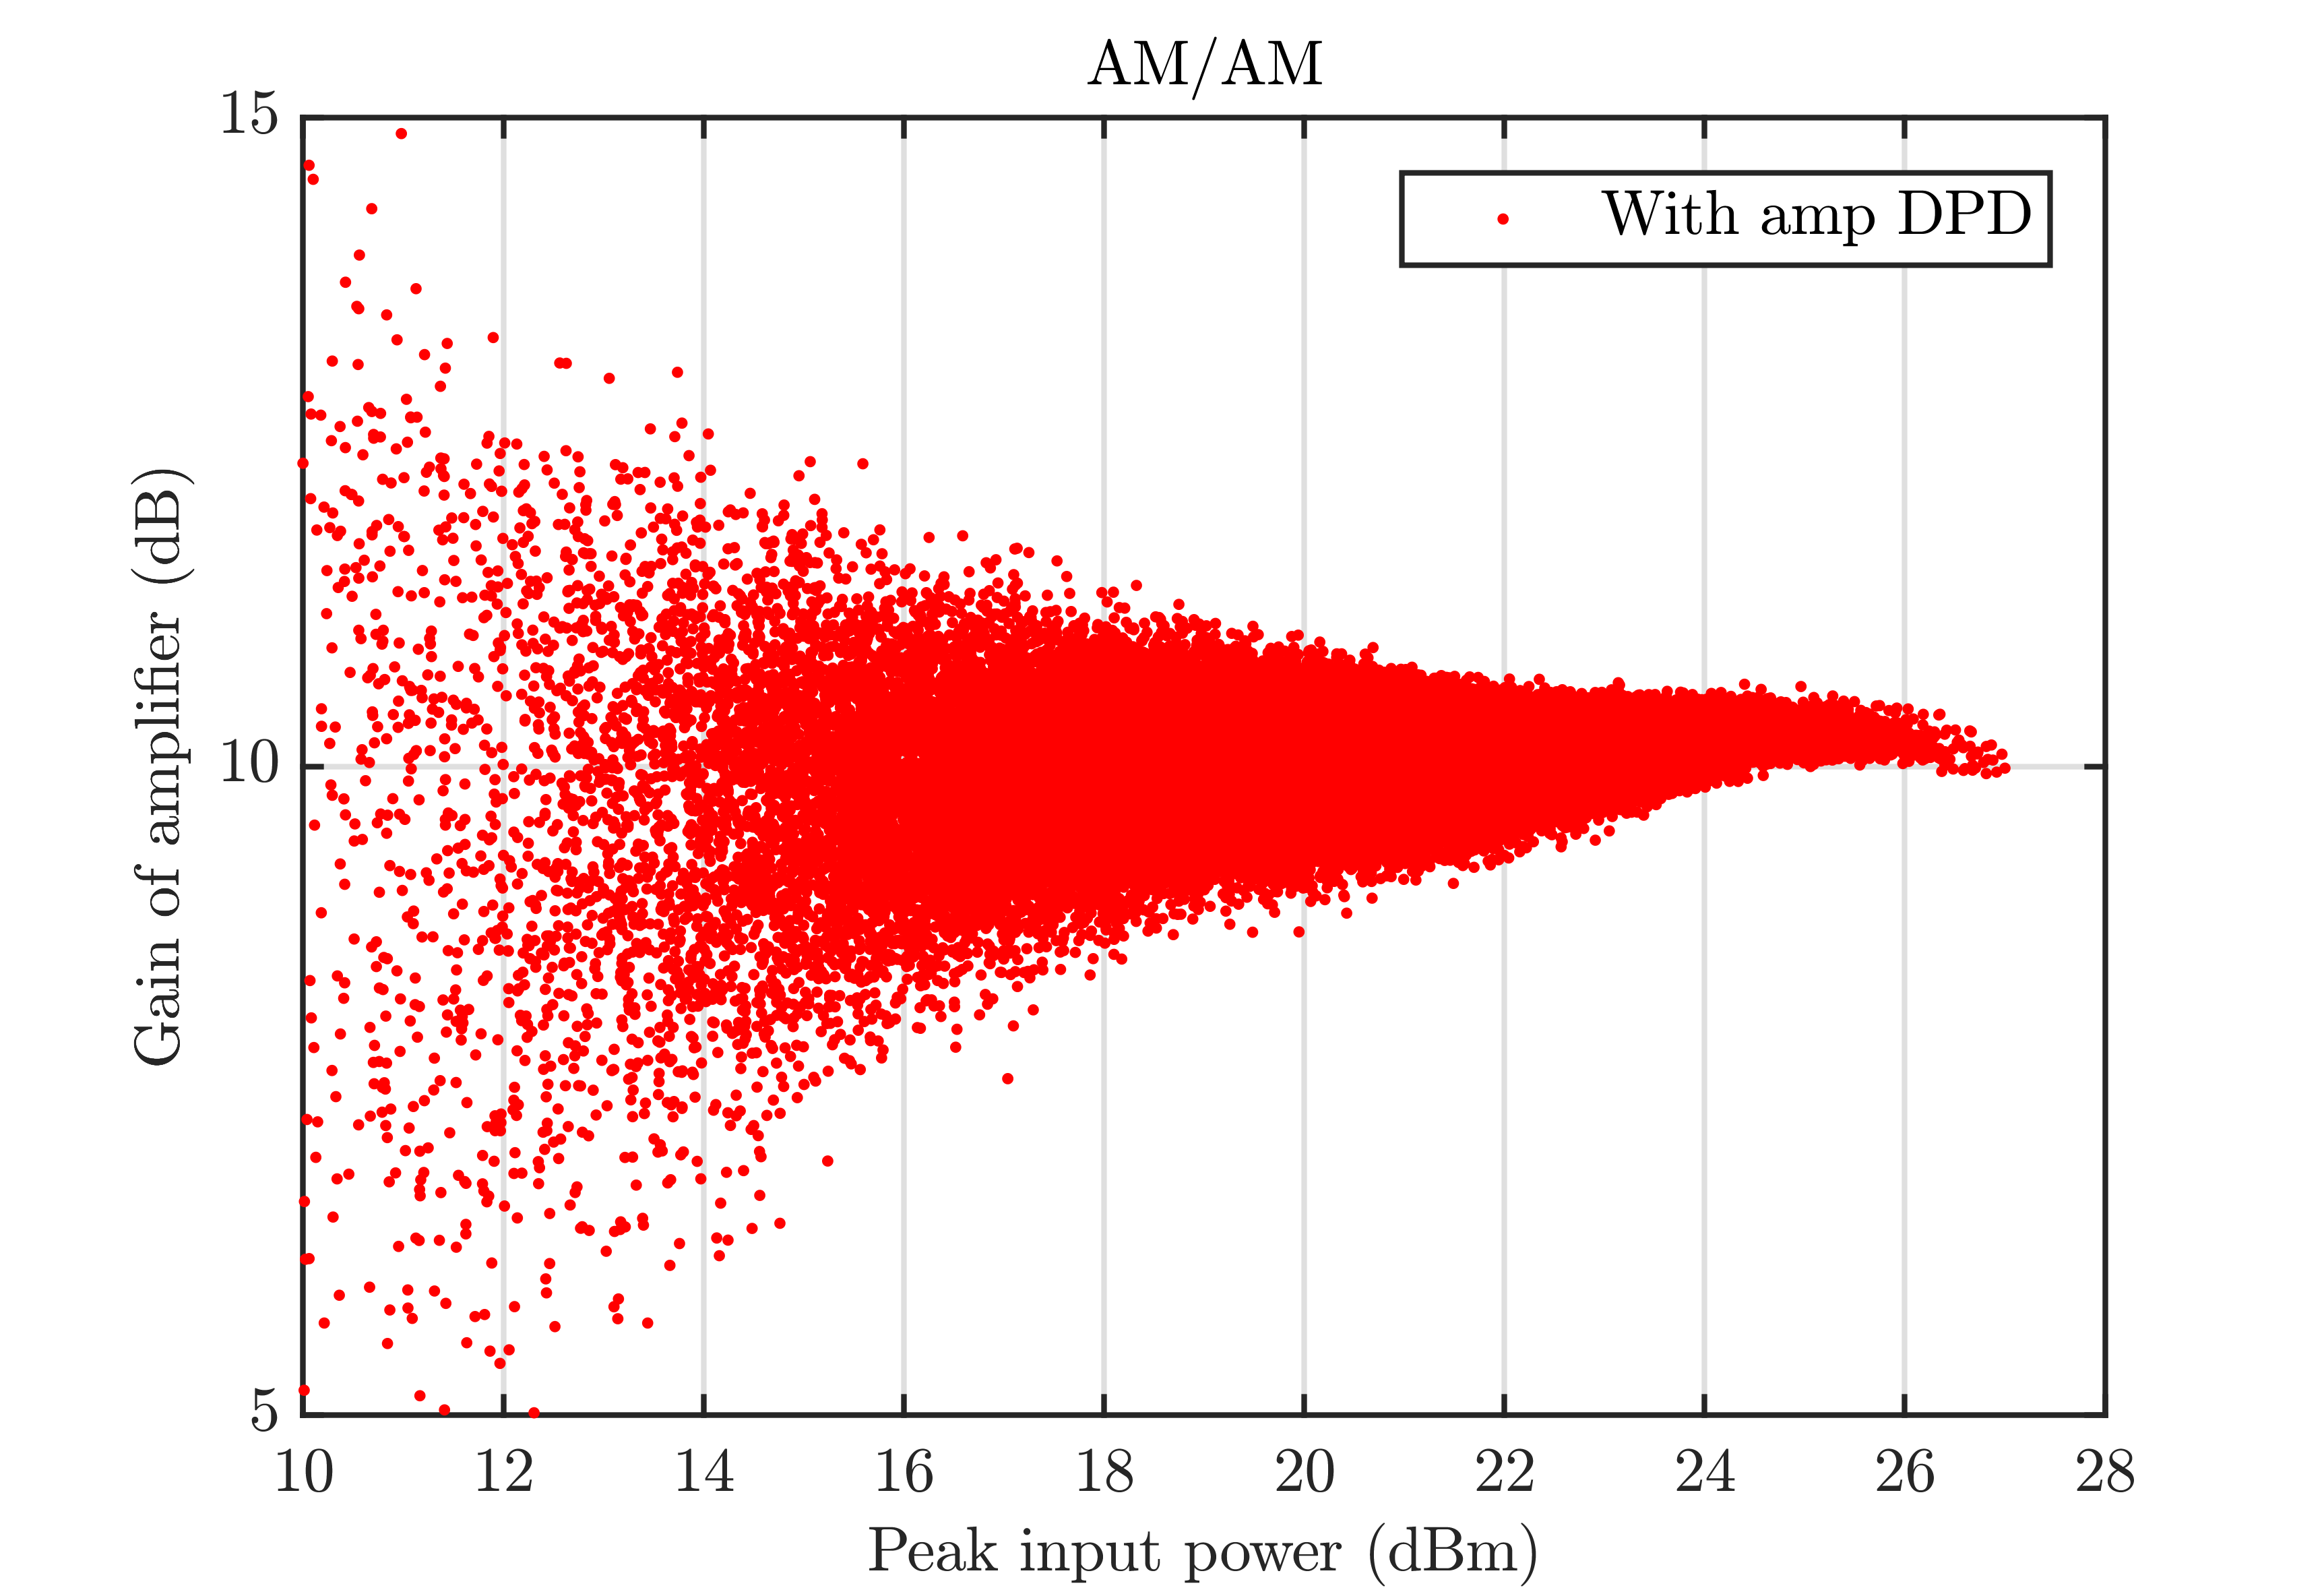
\includegraphics[scale = 0.5]{figures/measurement/cree/meas3/amam_amp_dpd_0p5.png}
	\caption{AM/AM distortion at $d = 0.5\lambda$ with amplifier DPD}	
    \label{fig:meas3_amam5_2}
  \end{minipage}
  \hfill
  \begin{minipage}[b]{0.4\textwidth}
	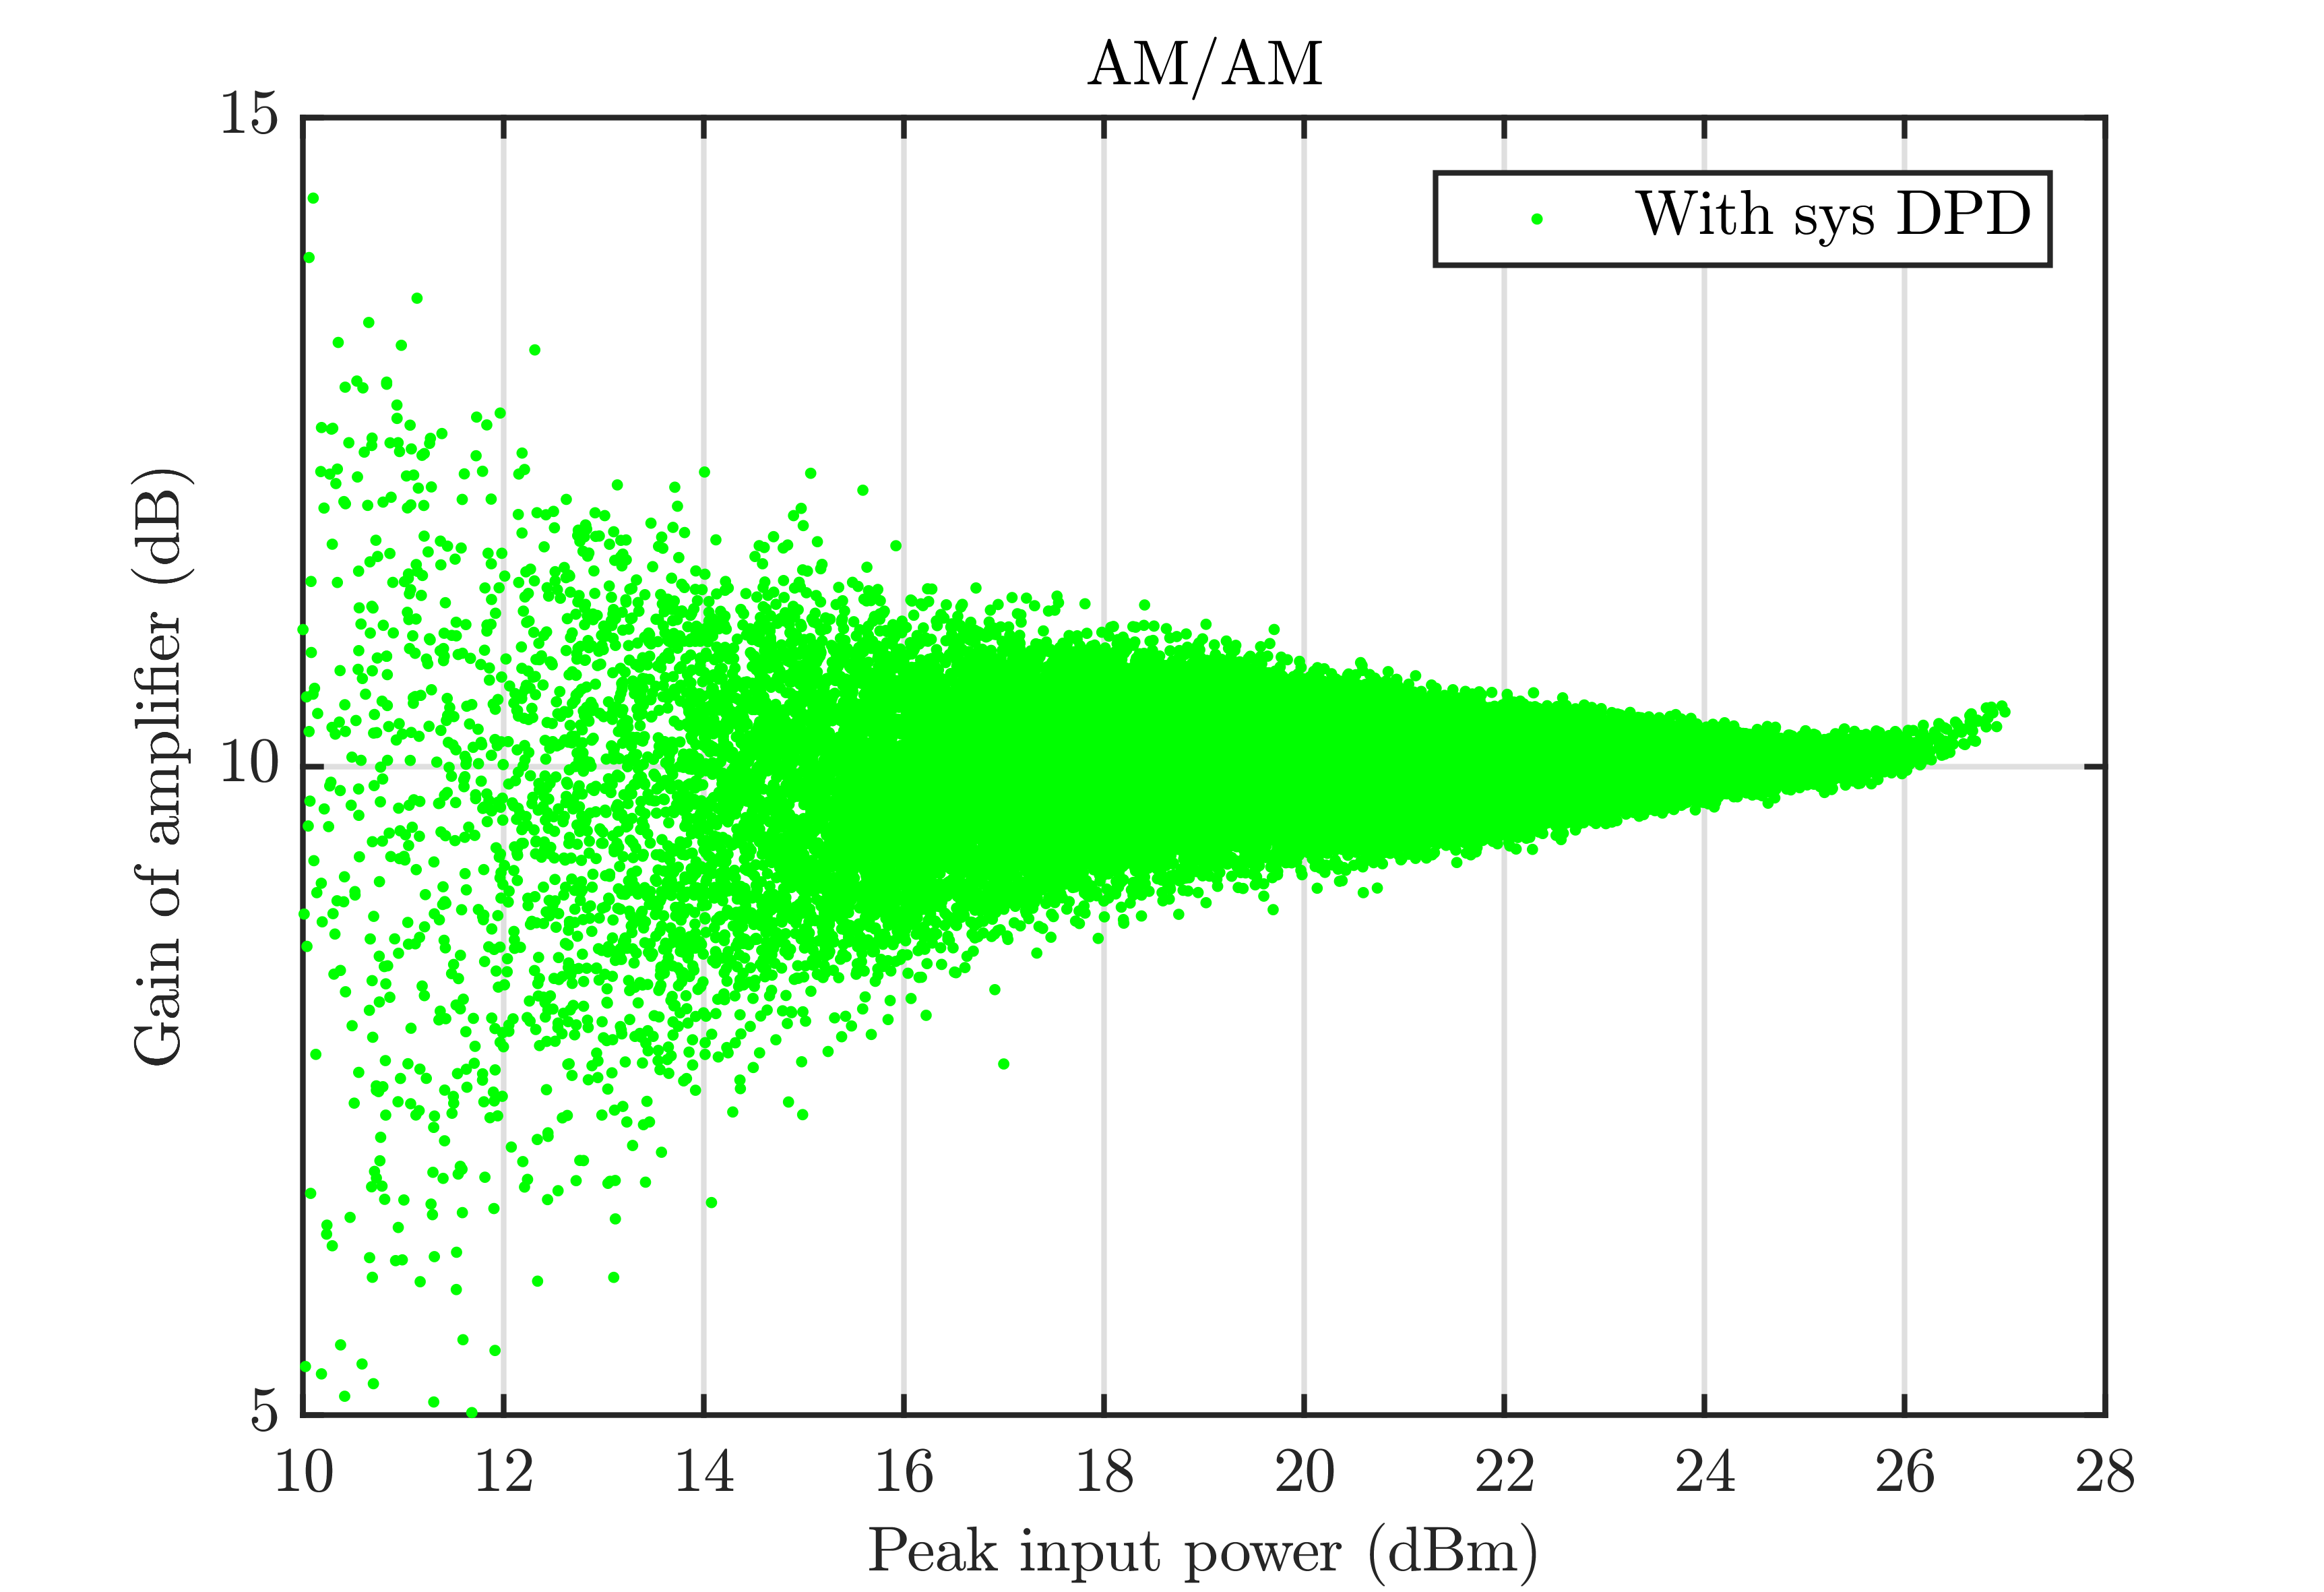
\includegraphics[scale = 0.5]{figures/measurement/cree/meas3/amam_sys_dpd_0p5.png}
	\caption{AM/AM distortion at $d = 0.5\lambda$ with system DPD}
    \label{fig:meas3_amam6_2}
  \end{minipage}
\end{figure}

\begin{figure}[H]
  \centering
  \begin{minipage}[b]{0.5\textwidth}
	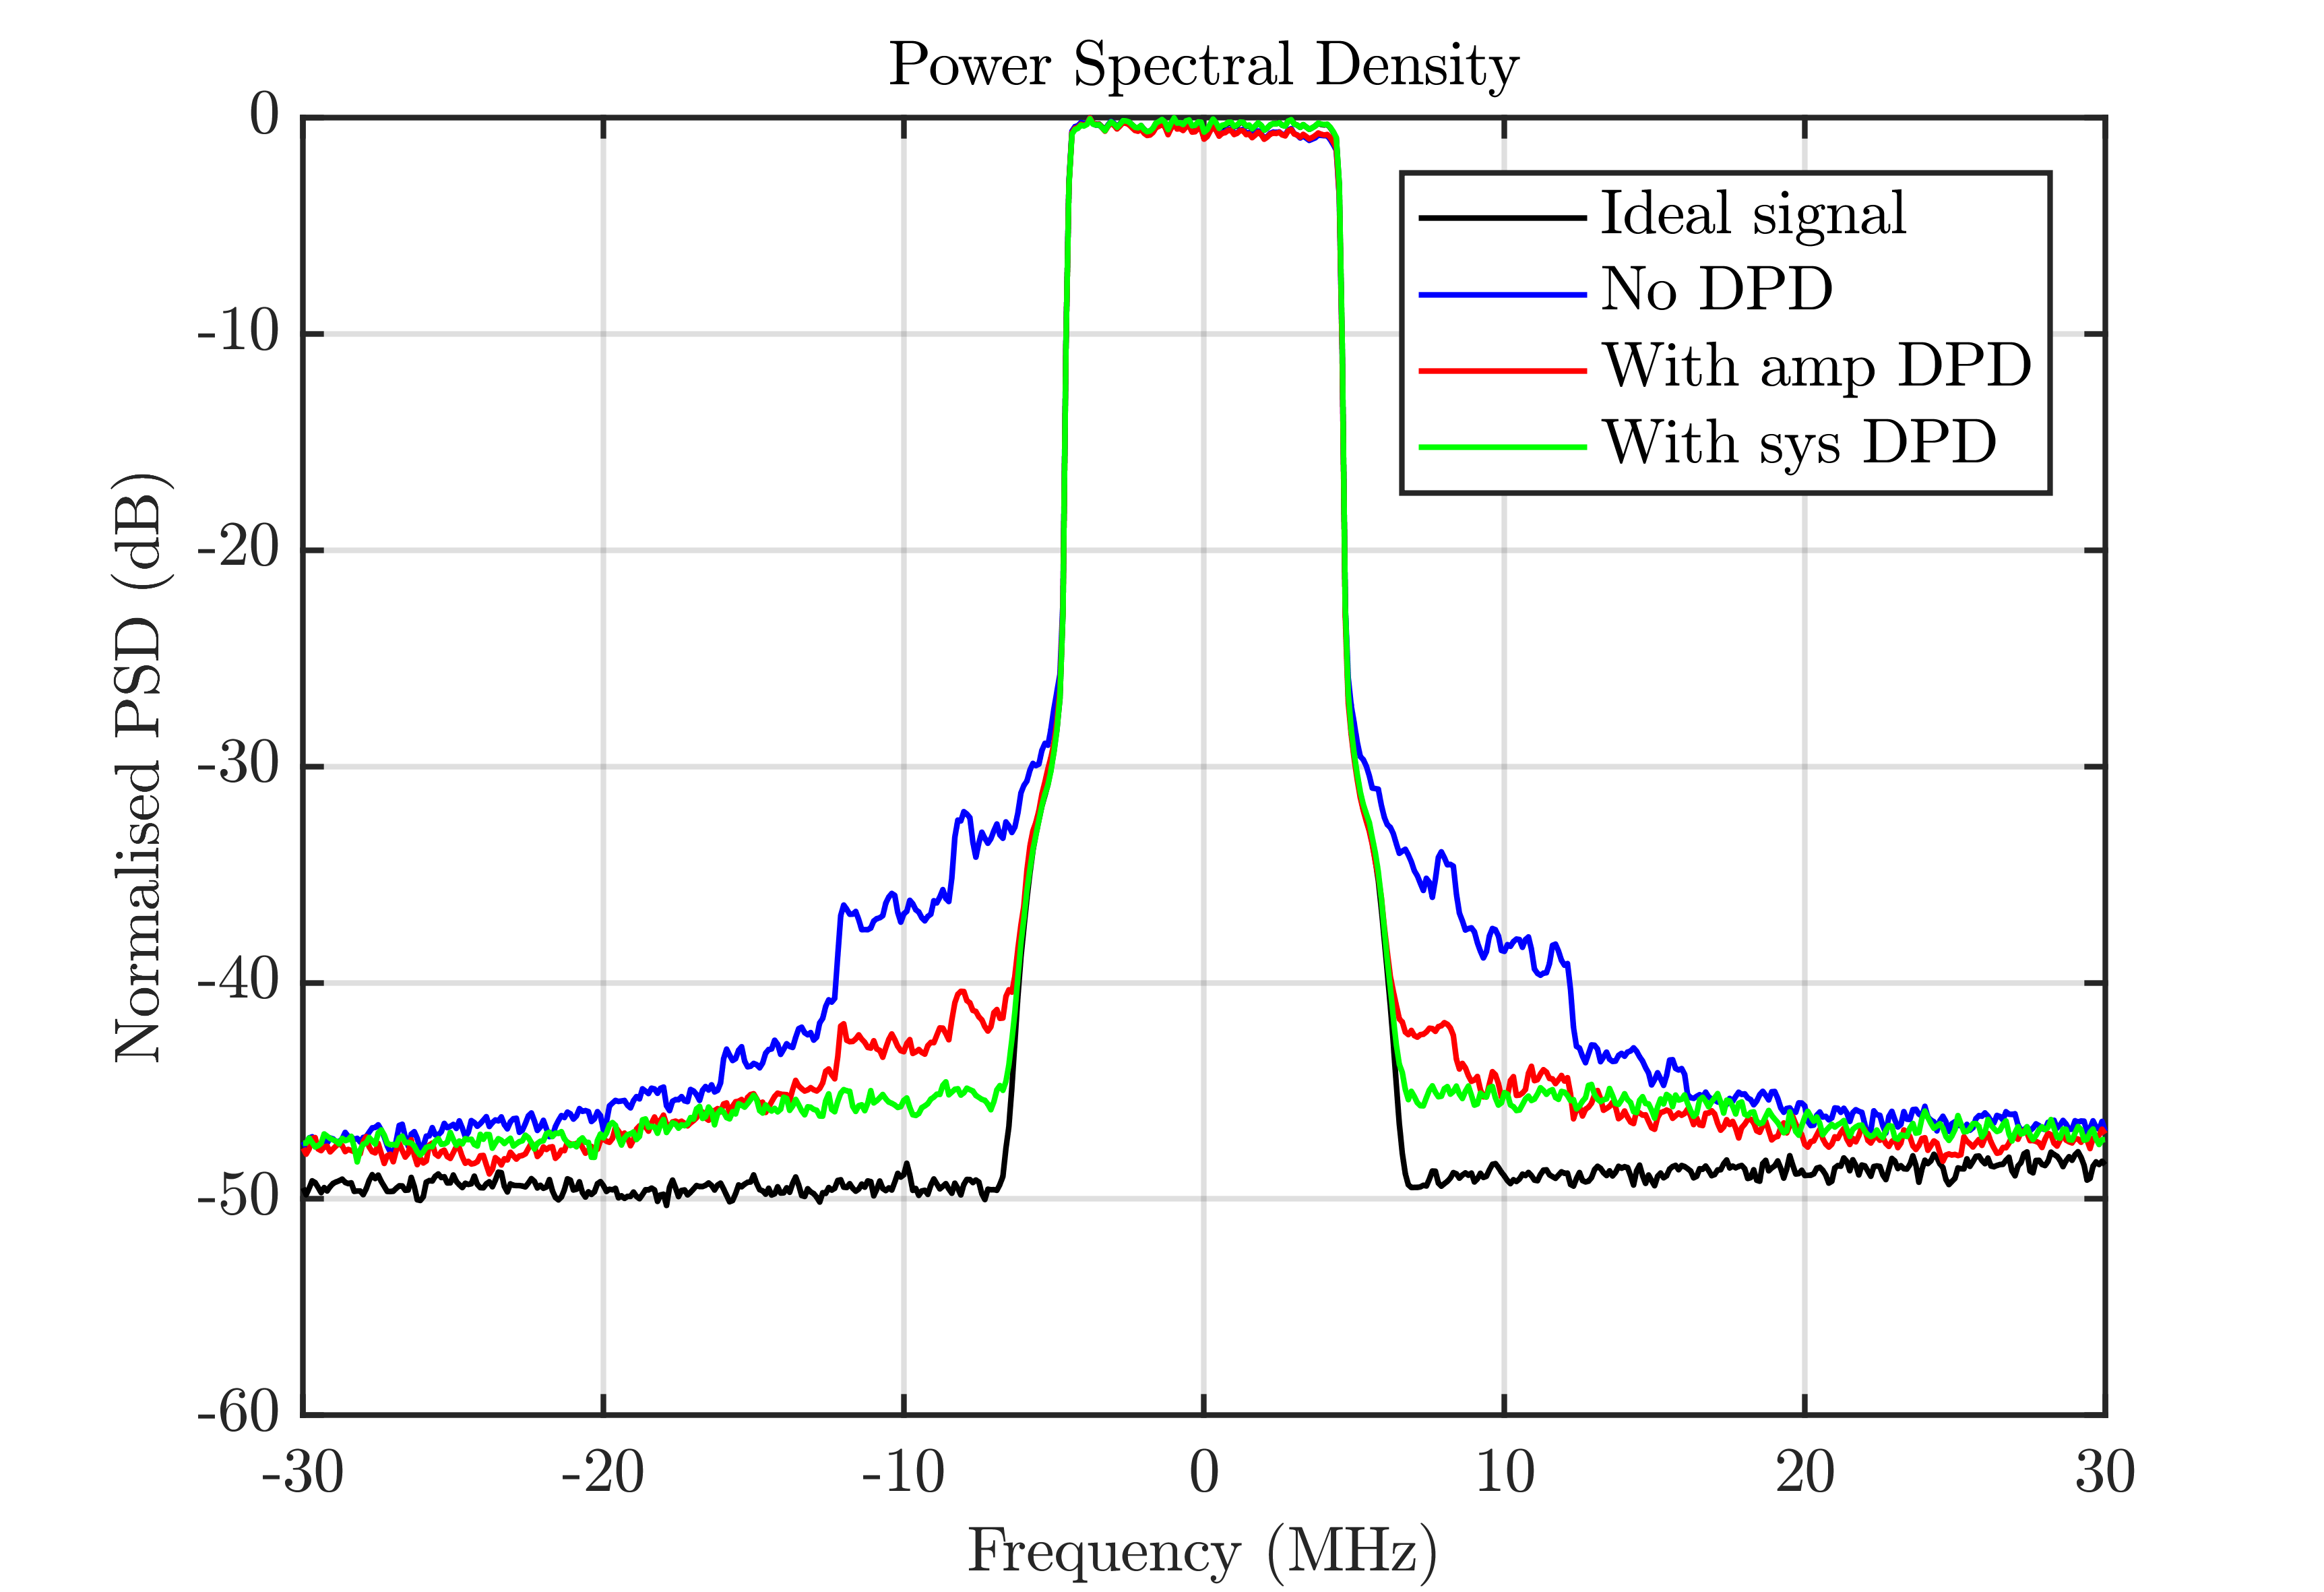
\includegraphics[scale = 0.5]{figures/measurement/cree/meas3/psd_0p5.png}
	\caption{PSD of measurement at $d = 0.5\lambda$ }	
    \label{fig:meas3_psd3_2}
  \end{minipage}
  \hfill
  \begin{minipage}[b]{0.4\textwidth}
	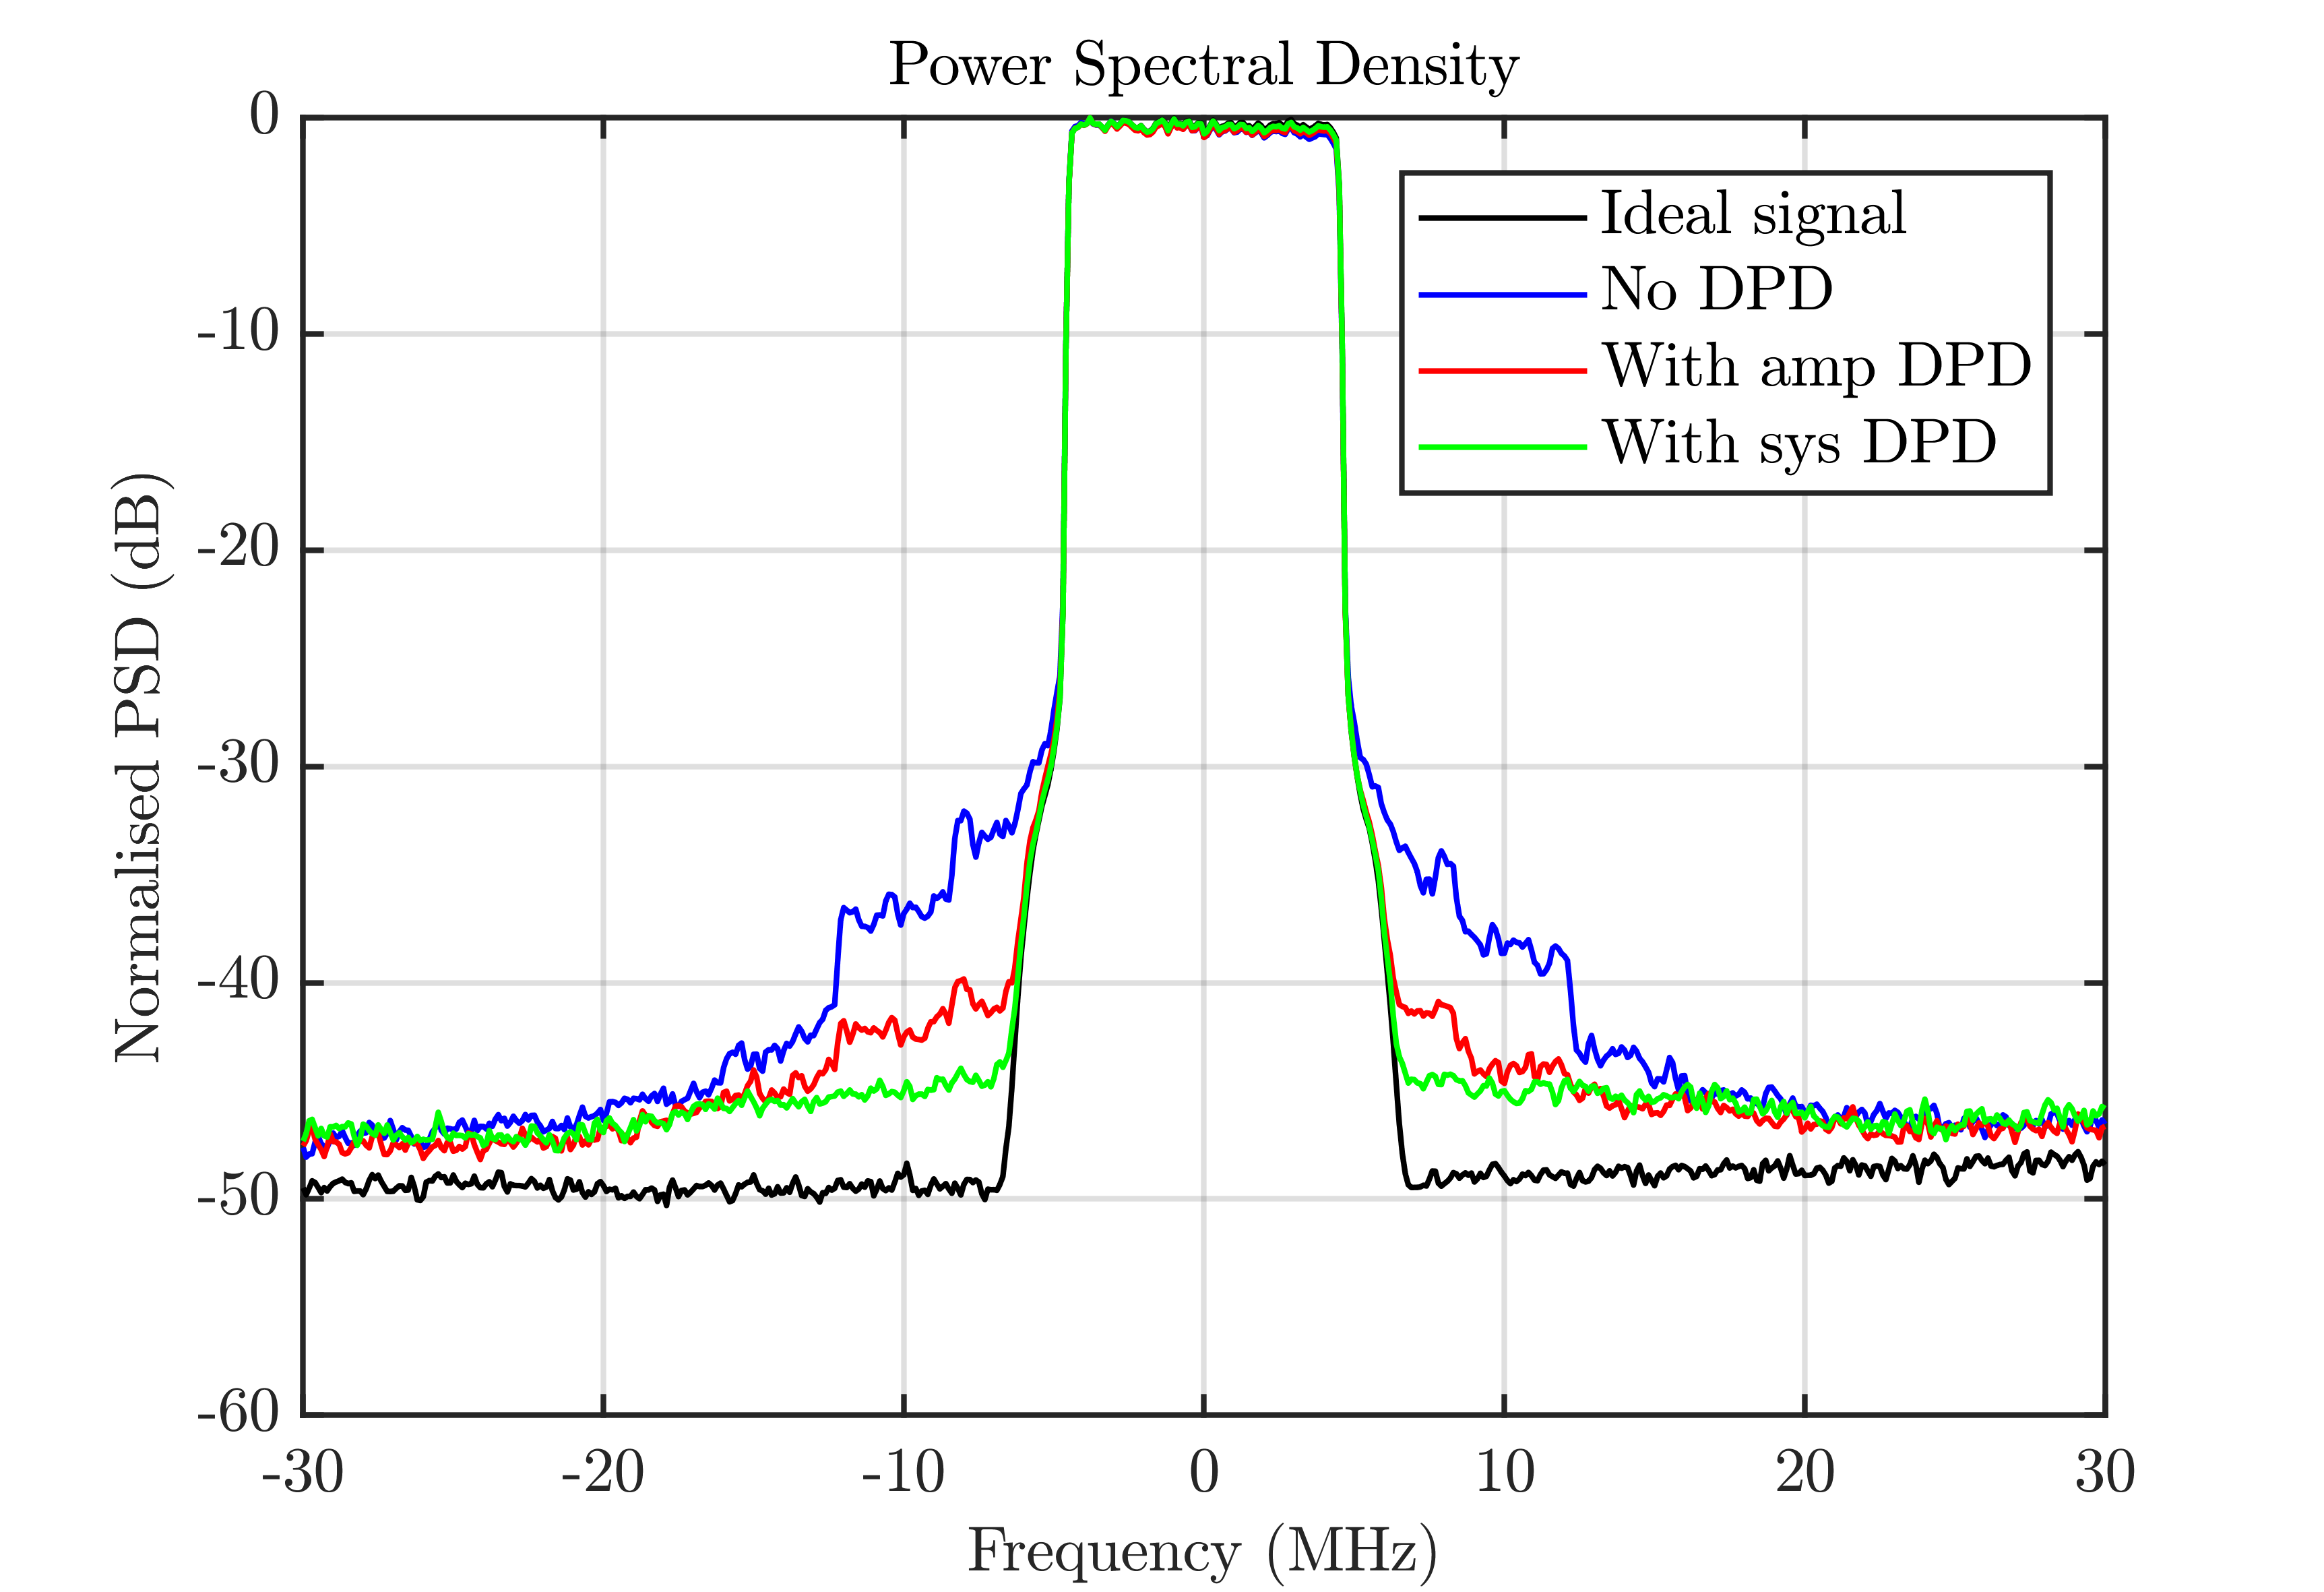
\includegraphics[scale = 0.5]{figures/measurement/cree/meas3/psd_0p6.png}
	\caption{PSD of measurement at $d = 0.6\lambda$}
    \label{fig:meas3_psd4_2}
  \end{minipage}
\end{figure}


\begin{figure}[H]
  \centering
  \begin{minipage}[b]{0.5\textwidth}
	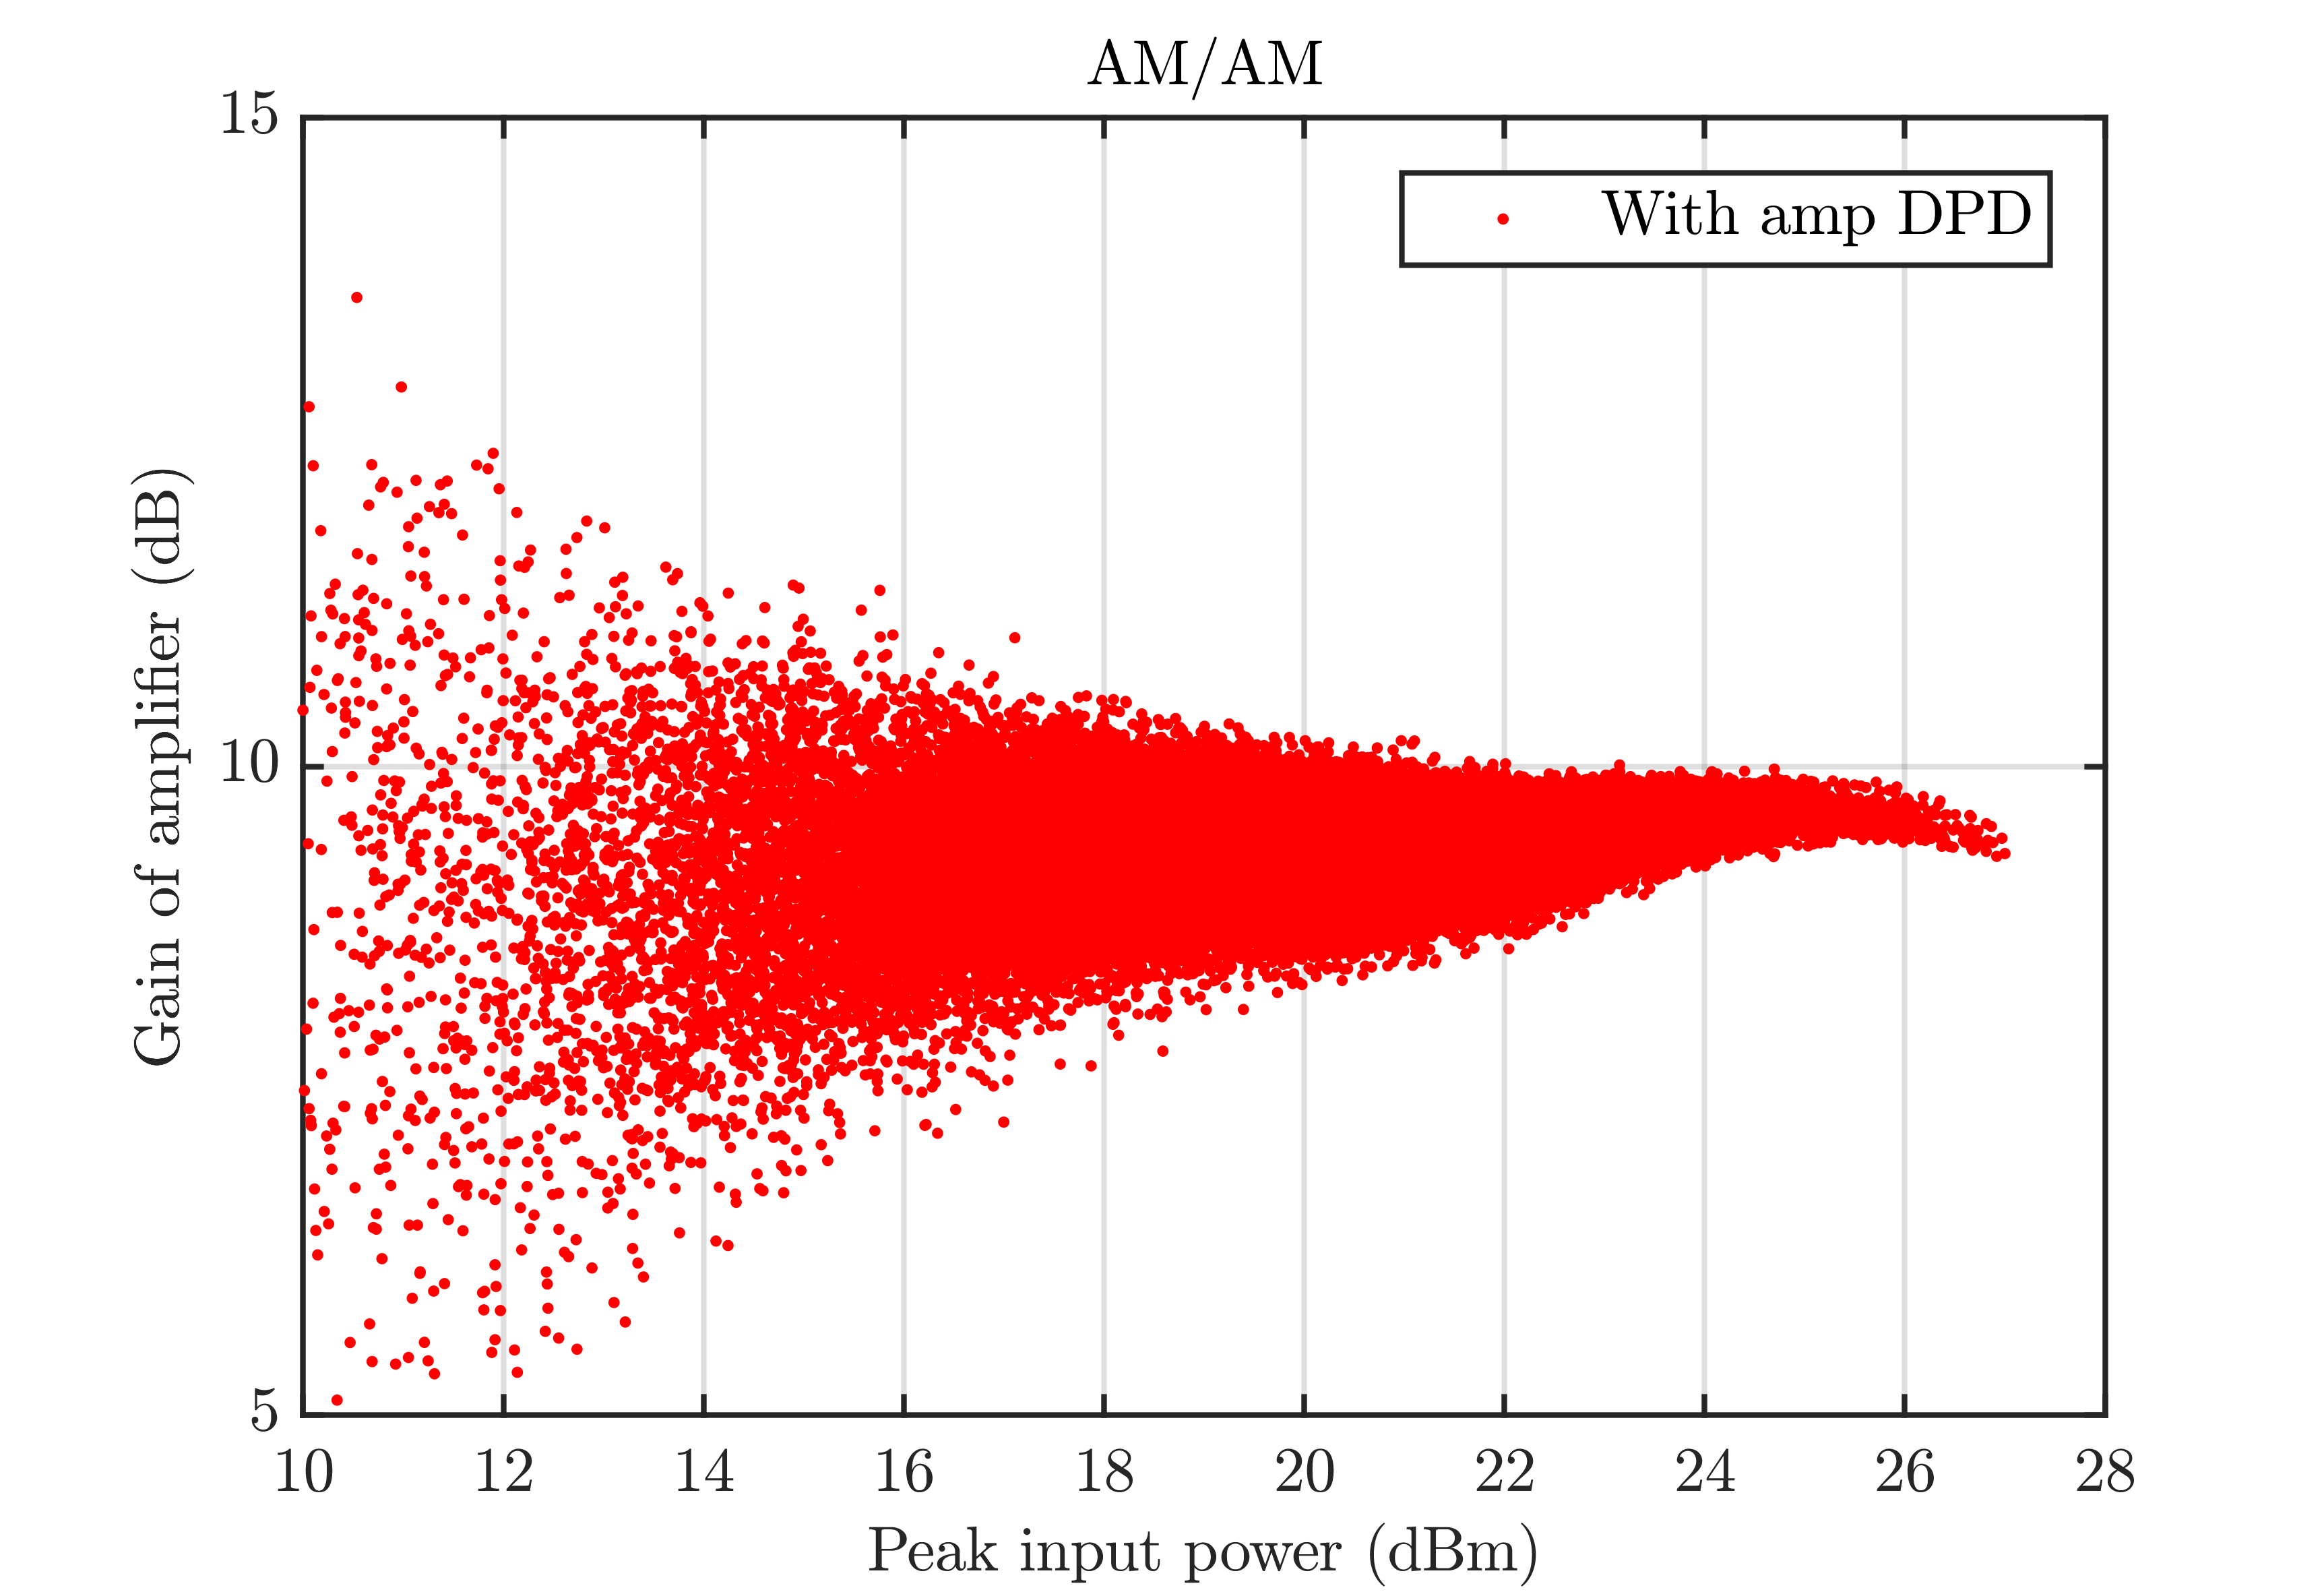
\includegraphics[scale = 0.5]{figures/measurement/cree/meas3/amam_amp_dpd_0p6.png}
	\caption{AM/AM distortion at $d = 0.6\lambda$ with amplifier DPD}	
    \label{fig:meas3_amam5_3}
  \end{minipage}
  \hfill
  \begin{minipage}[b]{0.4\textwidth}
	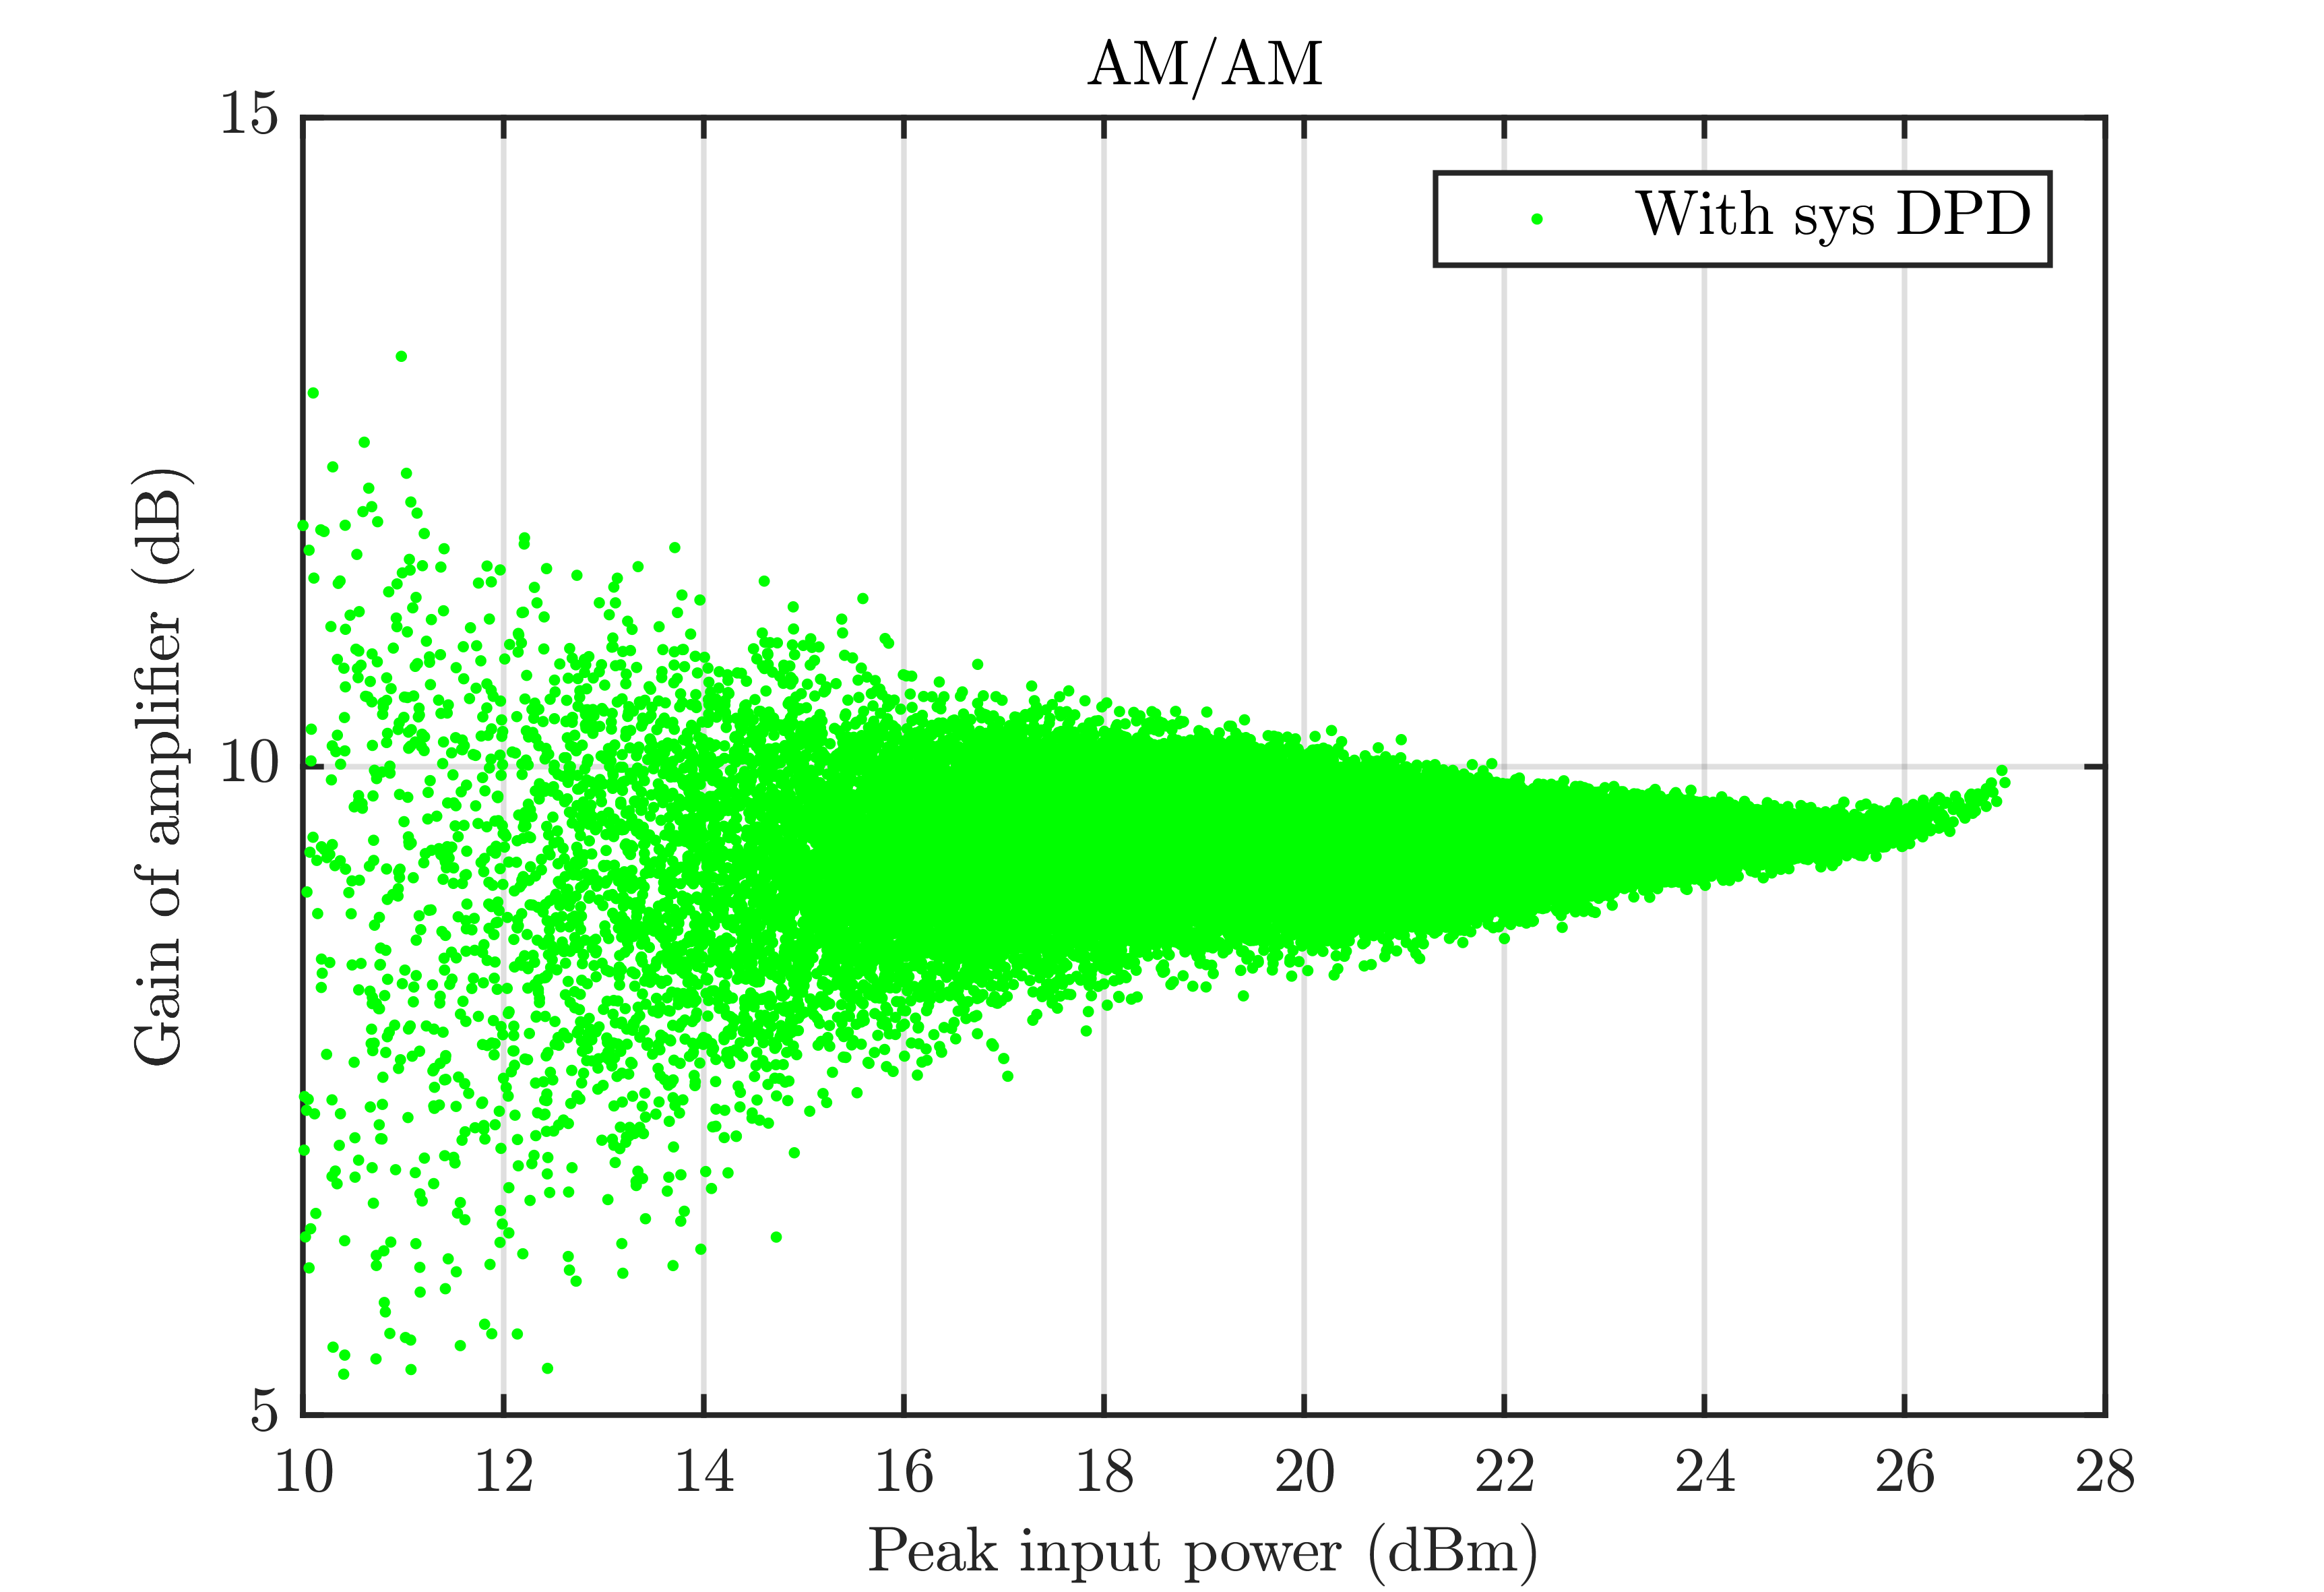
\includegraphics[scale = 0.5]{figures/measurement/cree/meas3/amam_sys_dpd_0p6.png}
	\caption{AM/AM distortion at $d = 0.6\lambda$ with system DPD}
    \label{fig:meas3_amam6_3}
  \end{minipage}
\end{figure}

\begin{figure}[H]
\centering 
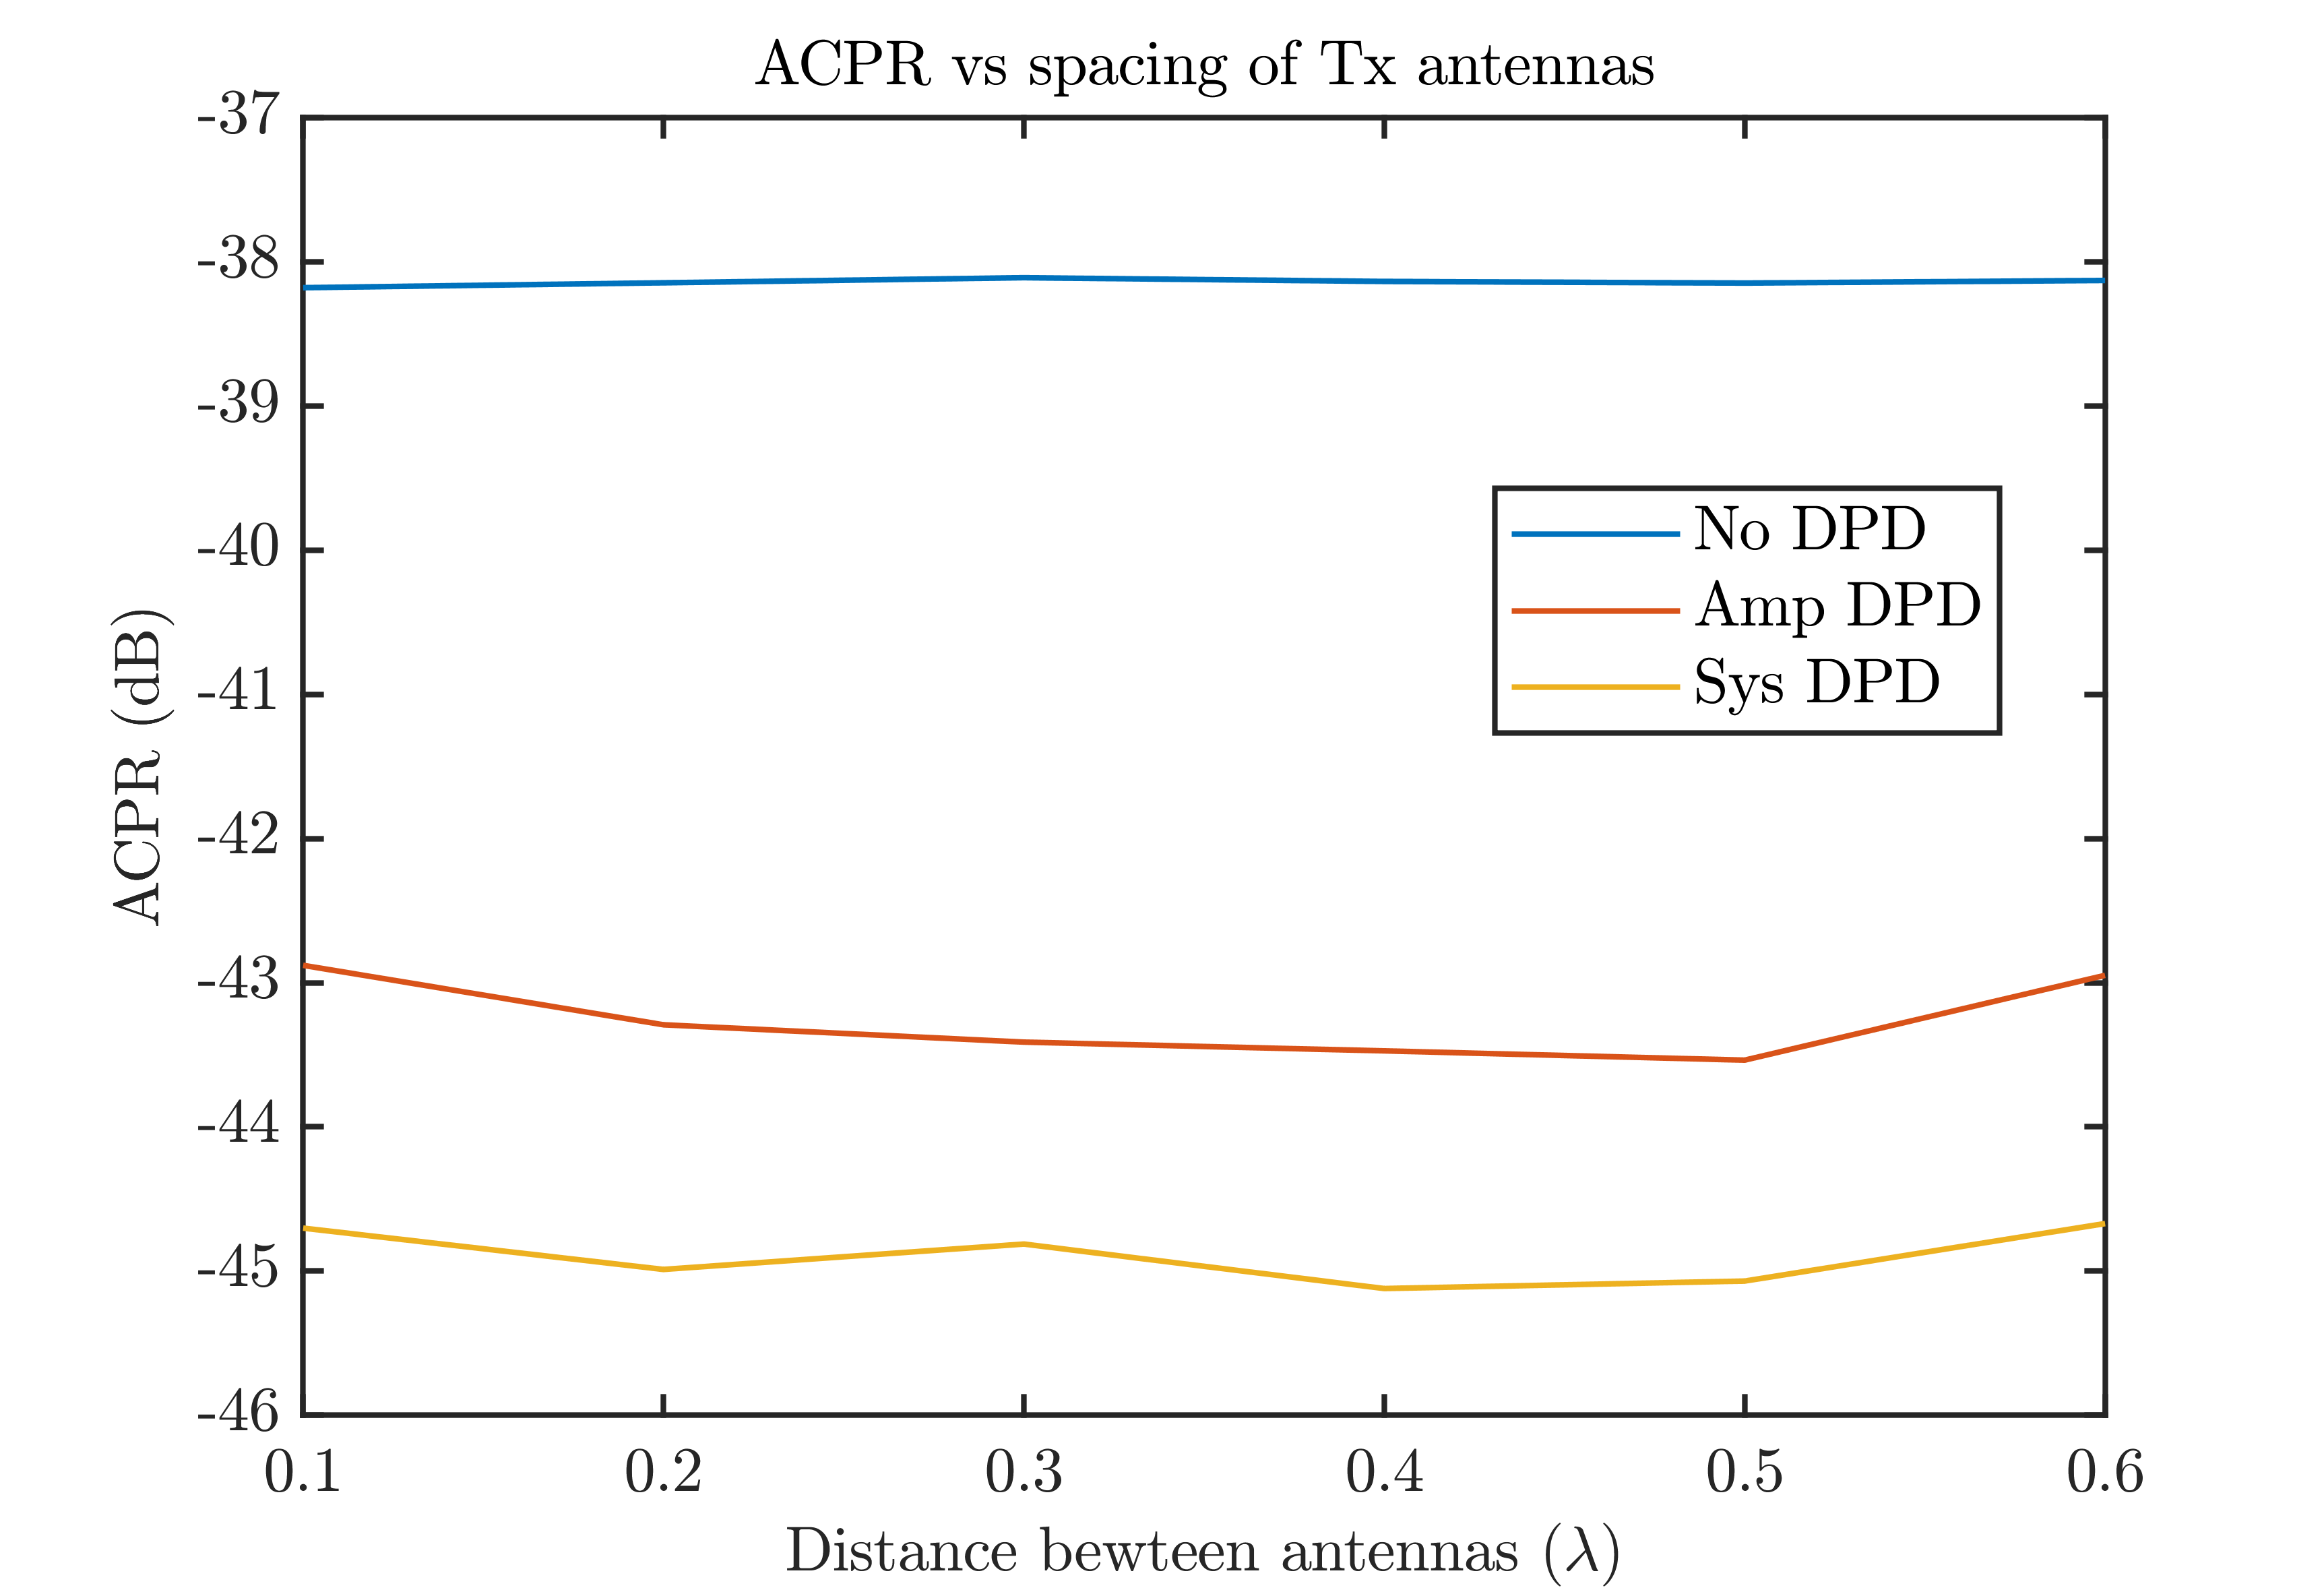
\includegraphics[scale = 0.6]{figures/measurement/cree/meas3/acpr_two_ant.png}
\caption{ACPR versus distance between antennas}
\label{fig:meas2_dpd}
\end{figure}

From the AM/AM plots it can be seen that when doing DPD with only the model for the amplifier taken into account,  there are lots of non-linearity about 22-27dBm input. When treating the amplifiers with antennas as one model the AM/AM linearity is improved but it seems that the DPD algorithm tends to overcompensate at high power values. From the PSD plots it is seen that the ACPR is decreased when treating the setup as one model. This can also be seen in figure \ref{fig:meas2_dpd} where the ACPR is shown for the diffrent distances. It is seen that the ACPR is close to -45dB for all distances and only small variations is seen. The small variations is caused by the difference in the antenna array, where the highest gain is at $0.5\lambda$ which then has the lowest ACPR for the ''Amp DPD''. The antenna measurement is presented in section \ref{ch:ant_meas}.    




%%%%%%%%%%%%%%%%%%%%%%%%%%%%%%%%%%%%%%%%%%%%%%%%%%%%%%%%%%%%%%%%%%%%%%%%%%%%%%%%%%%%%%%%%%%%%%%%%%%%%%%%%%%%%%%%

\section{Four amplifiers four antennas}

In this section measurement is done at four amplifiers and four antennas. The setup for the measurement is the same as in figure \ref{fig:meas_amp2} but with four amplifier branches instead of two. The results are shown in figure \ref{fig:meas_amp4} to \ref{fig:meas4_amam6_3}.

\begin{figure}[H]
\centering 
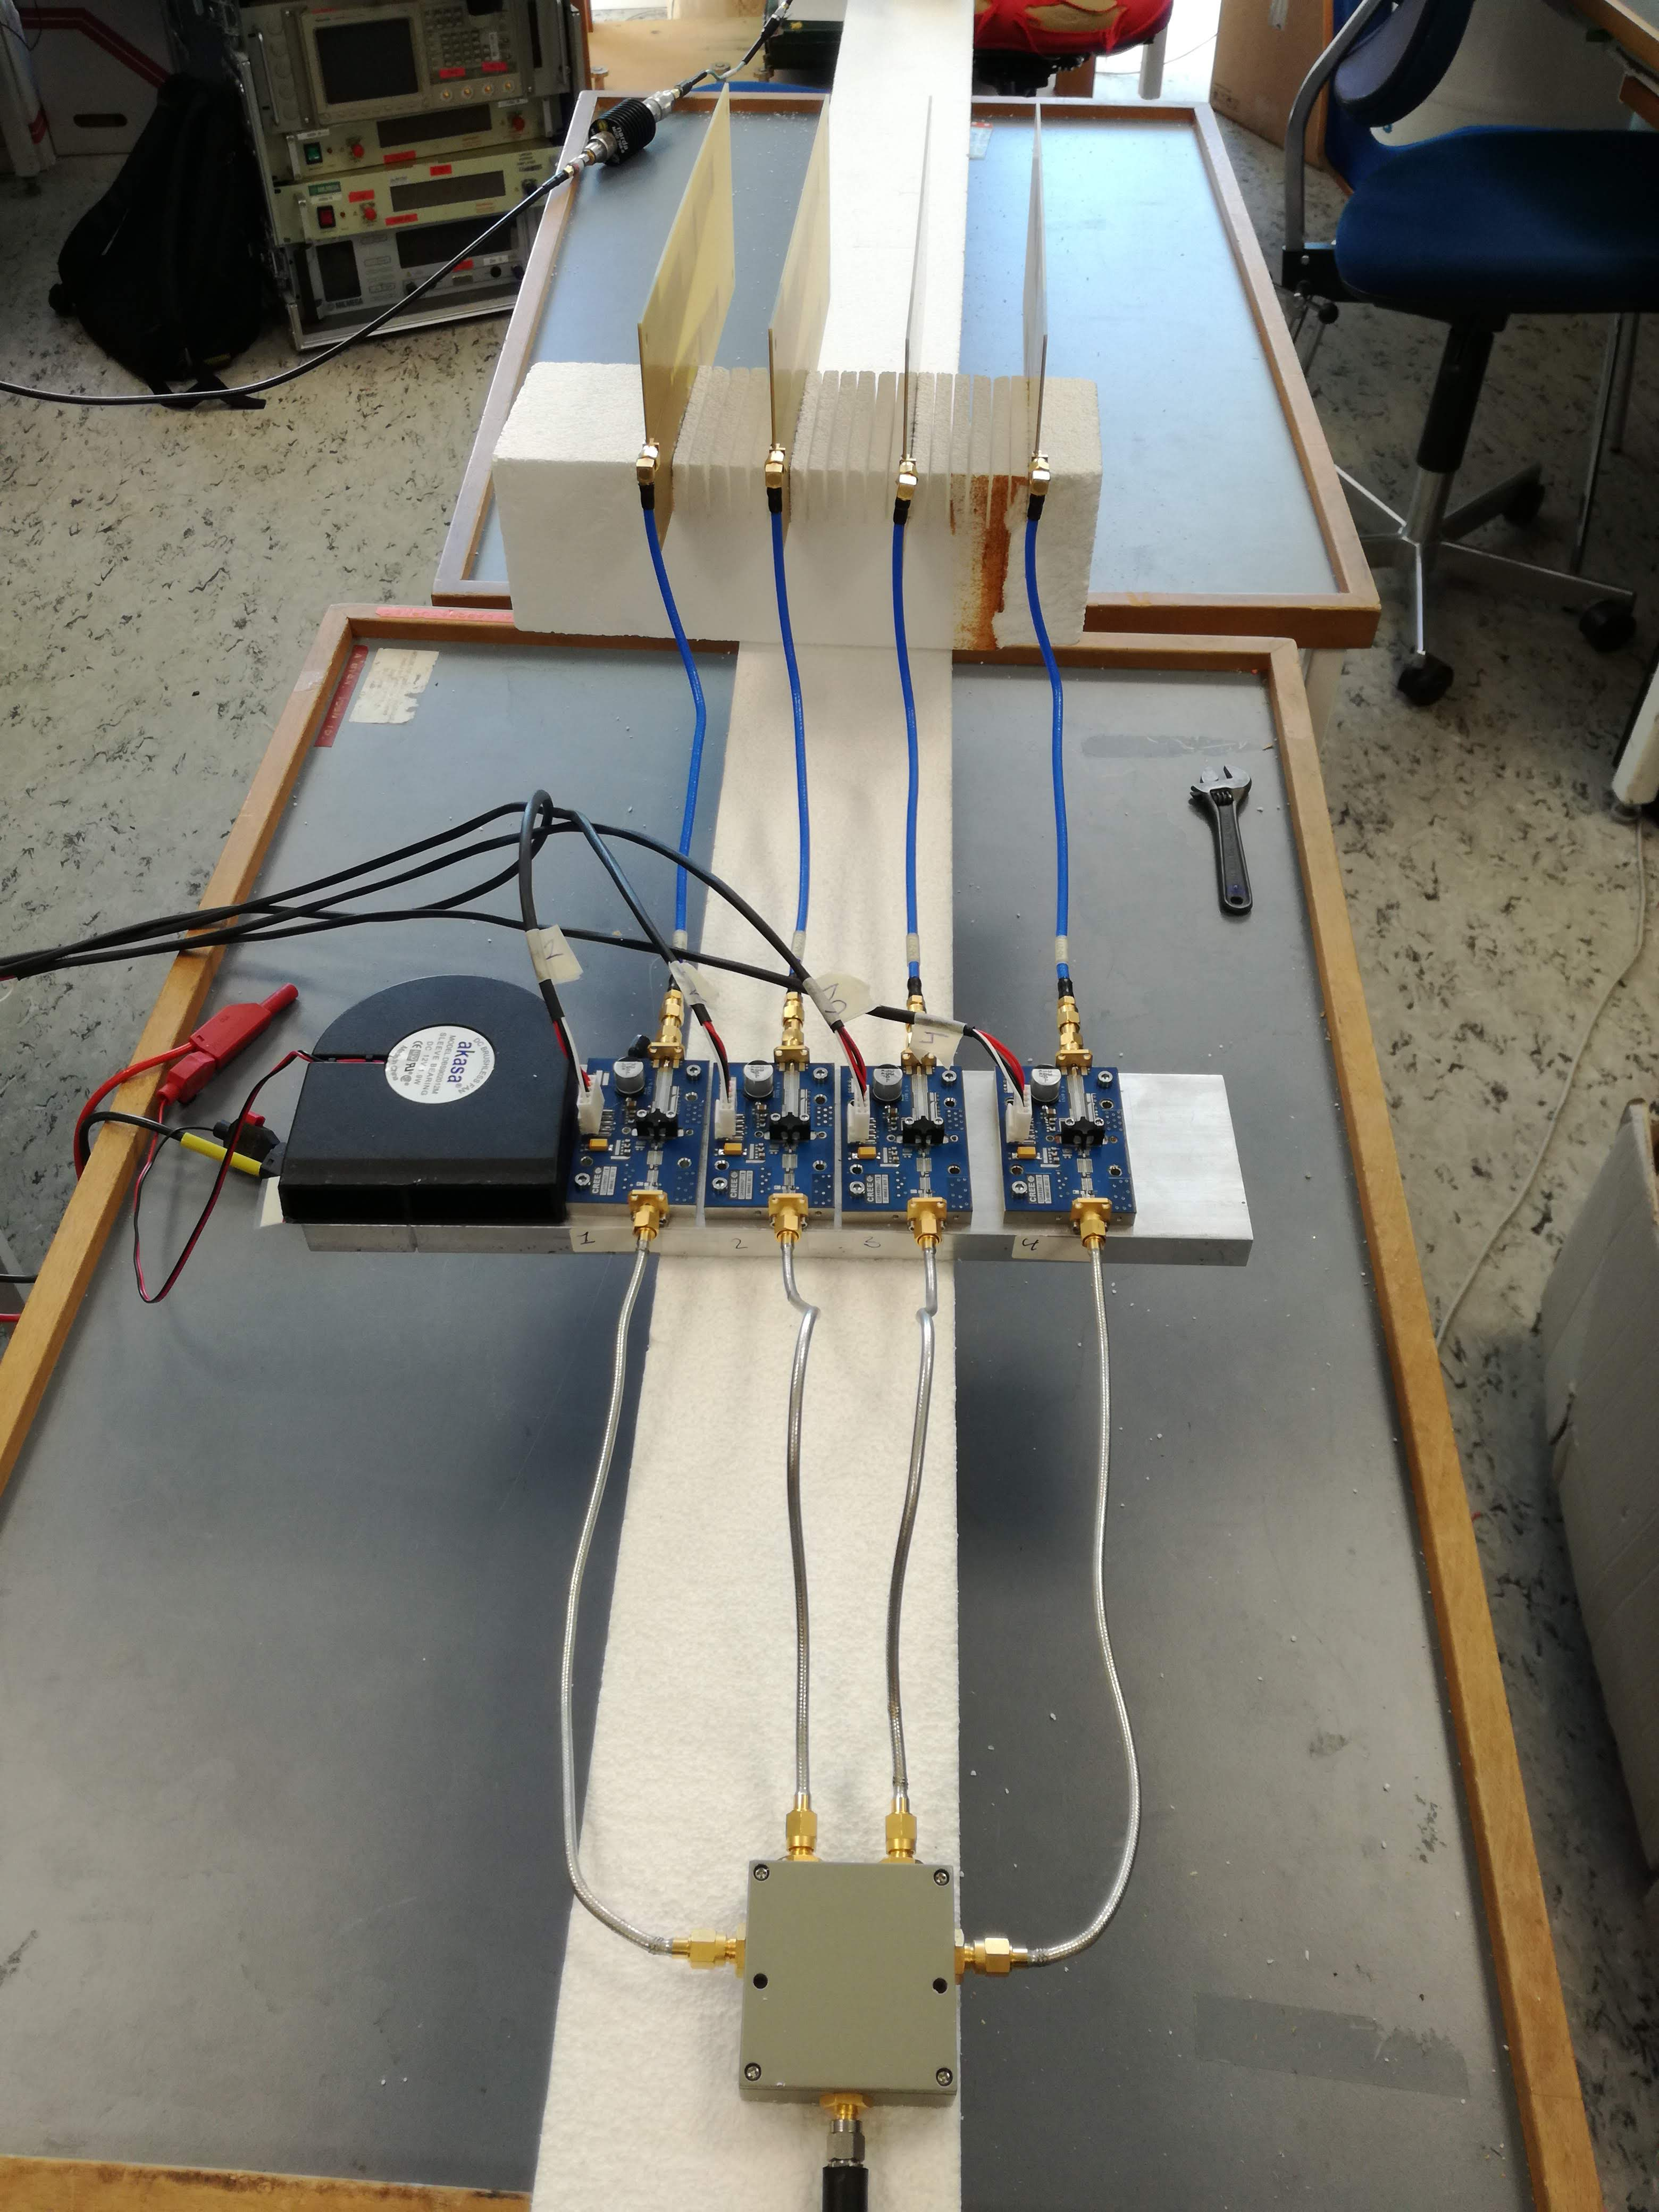
\includegraphics[scale = 0.1]{figures/measurement/cree/meas4/meas4.jpg}
\caption{Picture of measurement setup using four Tx antennas}
\label{fig:meas_amp4}
\end{figure}

\begin{figure}[H]
  \centering
  \begin{minipage}[b]{0.5\textwidth}
	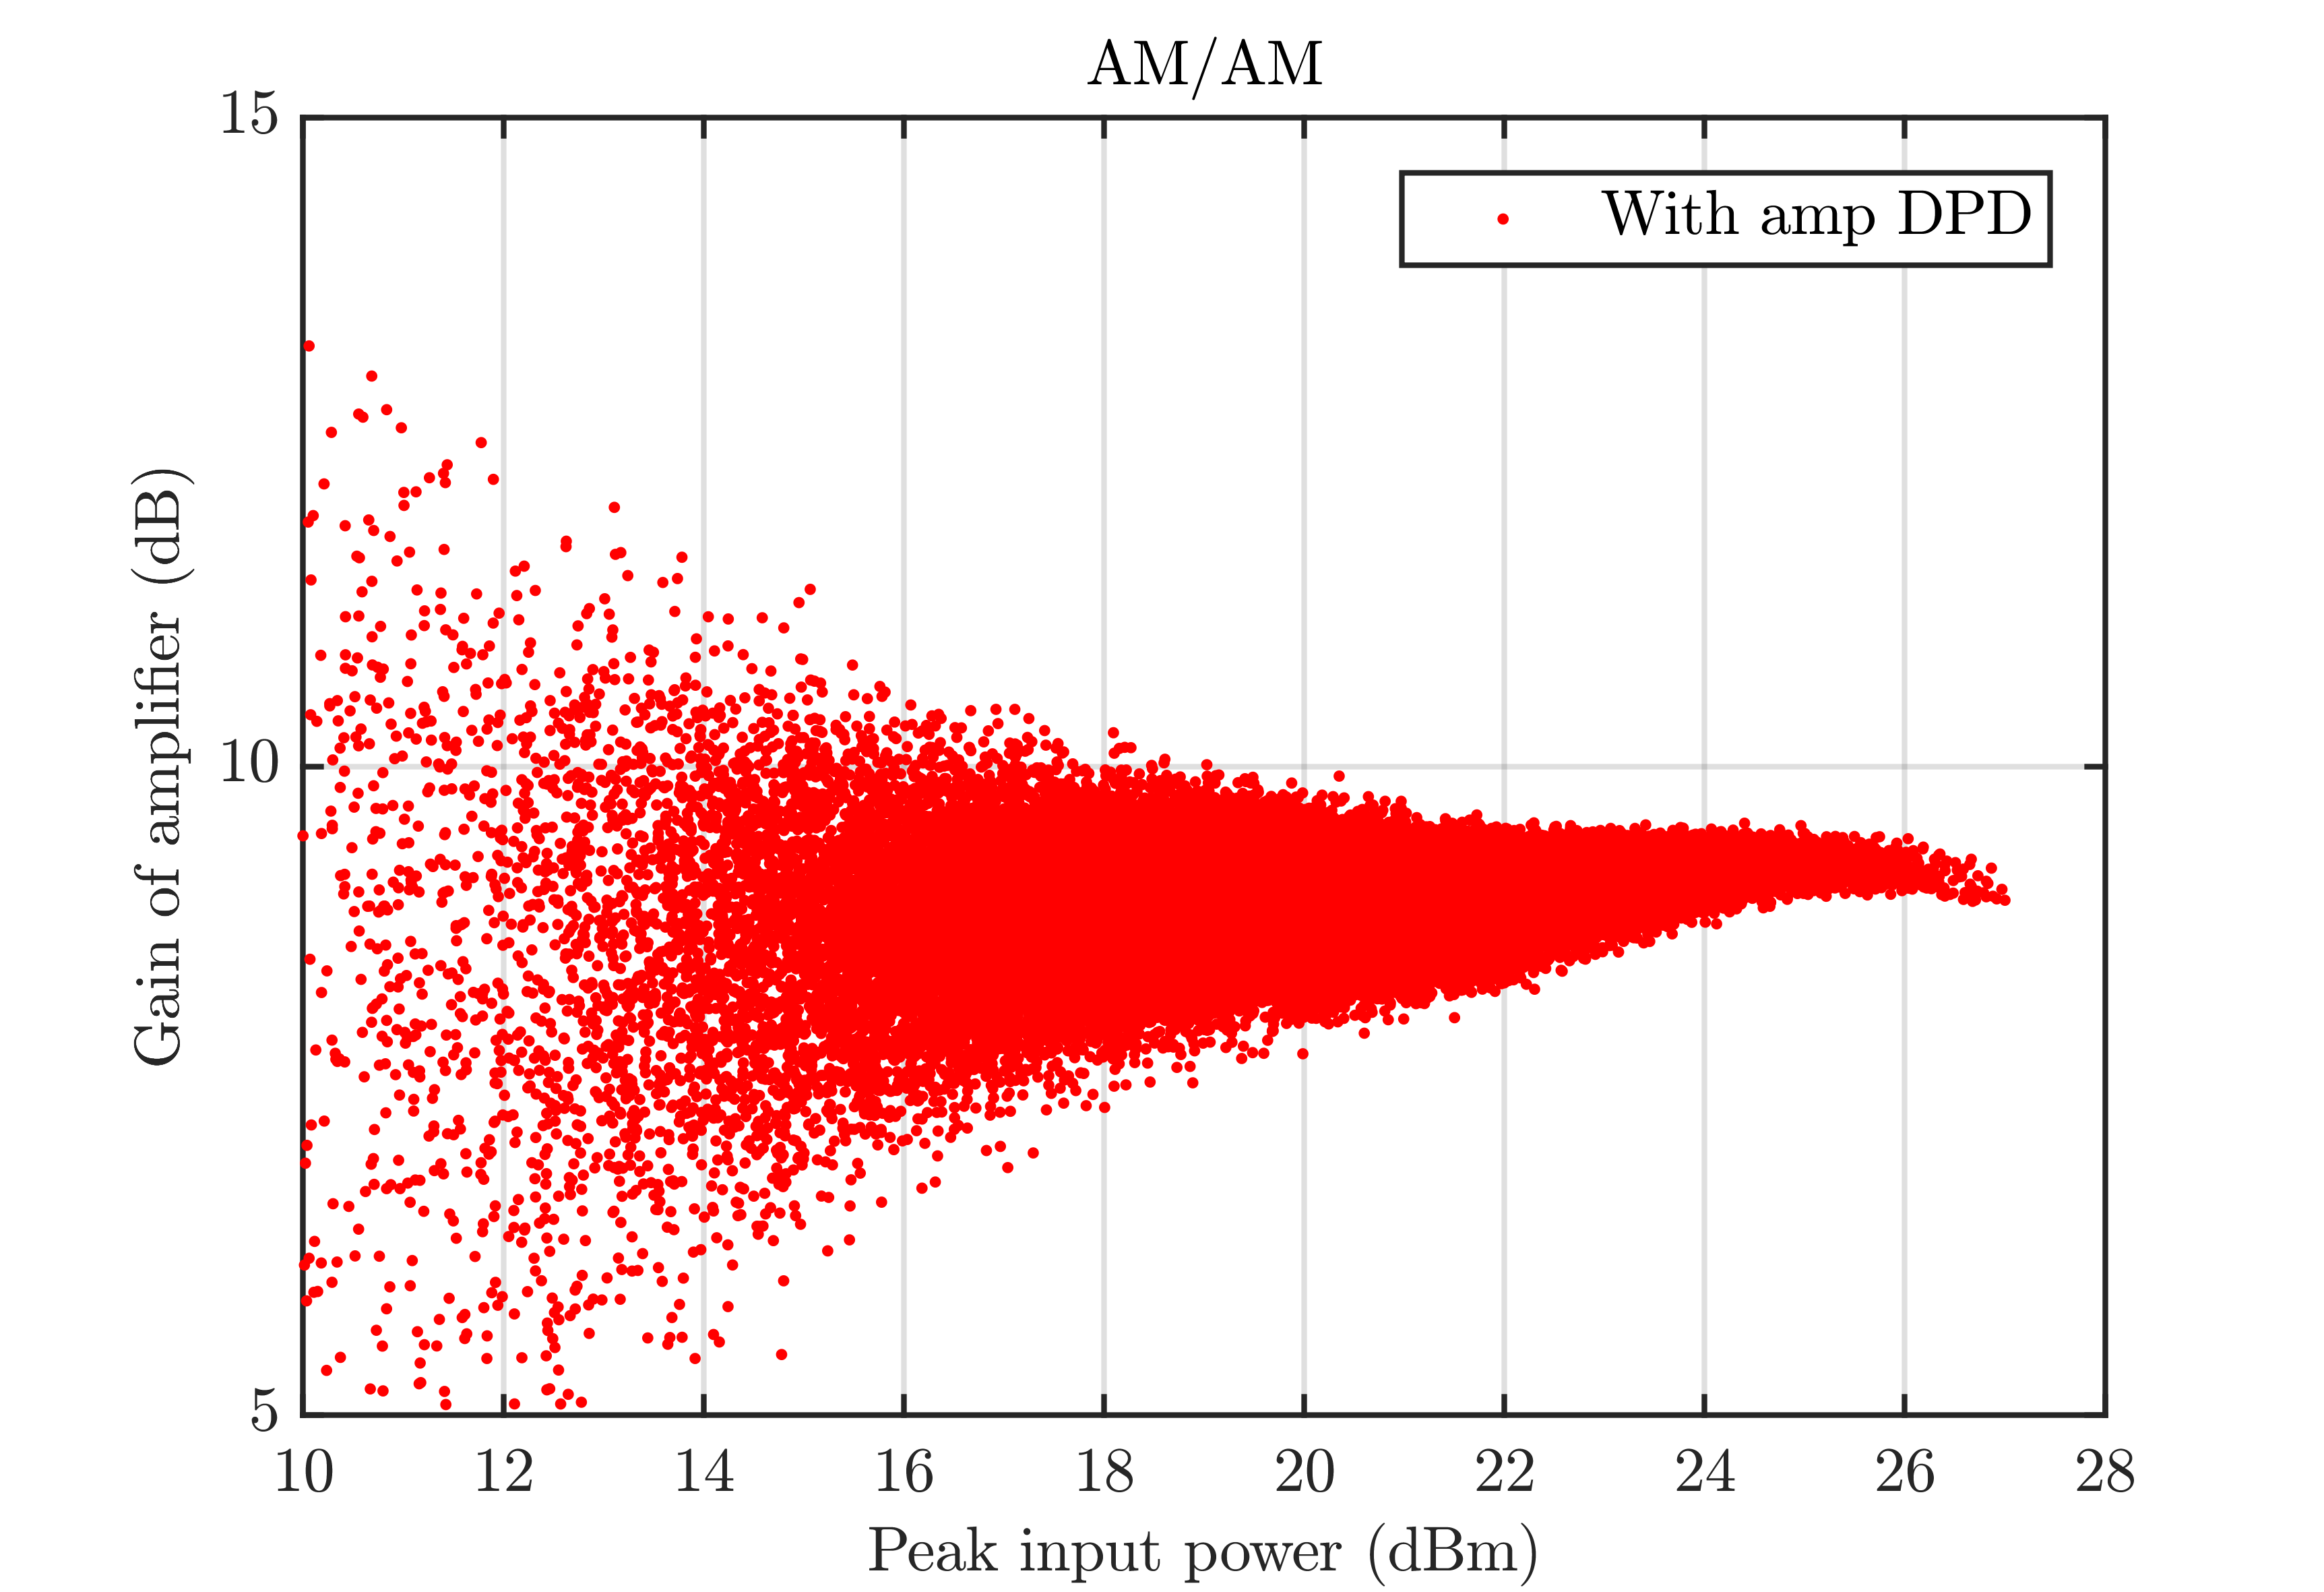
\includegraphics[scale = 0.5]{figures/measurement/cree/meas3/amam_amp_dpd_0p1.png}
	\caption{AM/AM distortion at $d = 0.1\lambda$ with amplifier DPD}	
    \label{fig:meas4_amam1}
  \end{minipage}
  \hfill
  \begin{minipage}[b]{0.4\textwidth}
	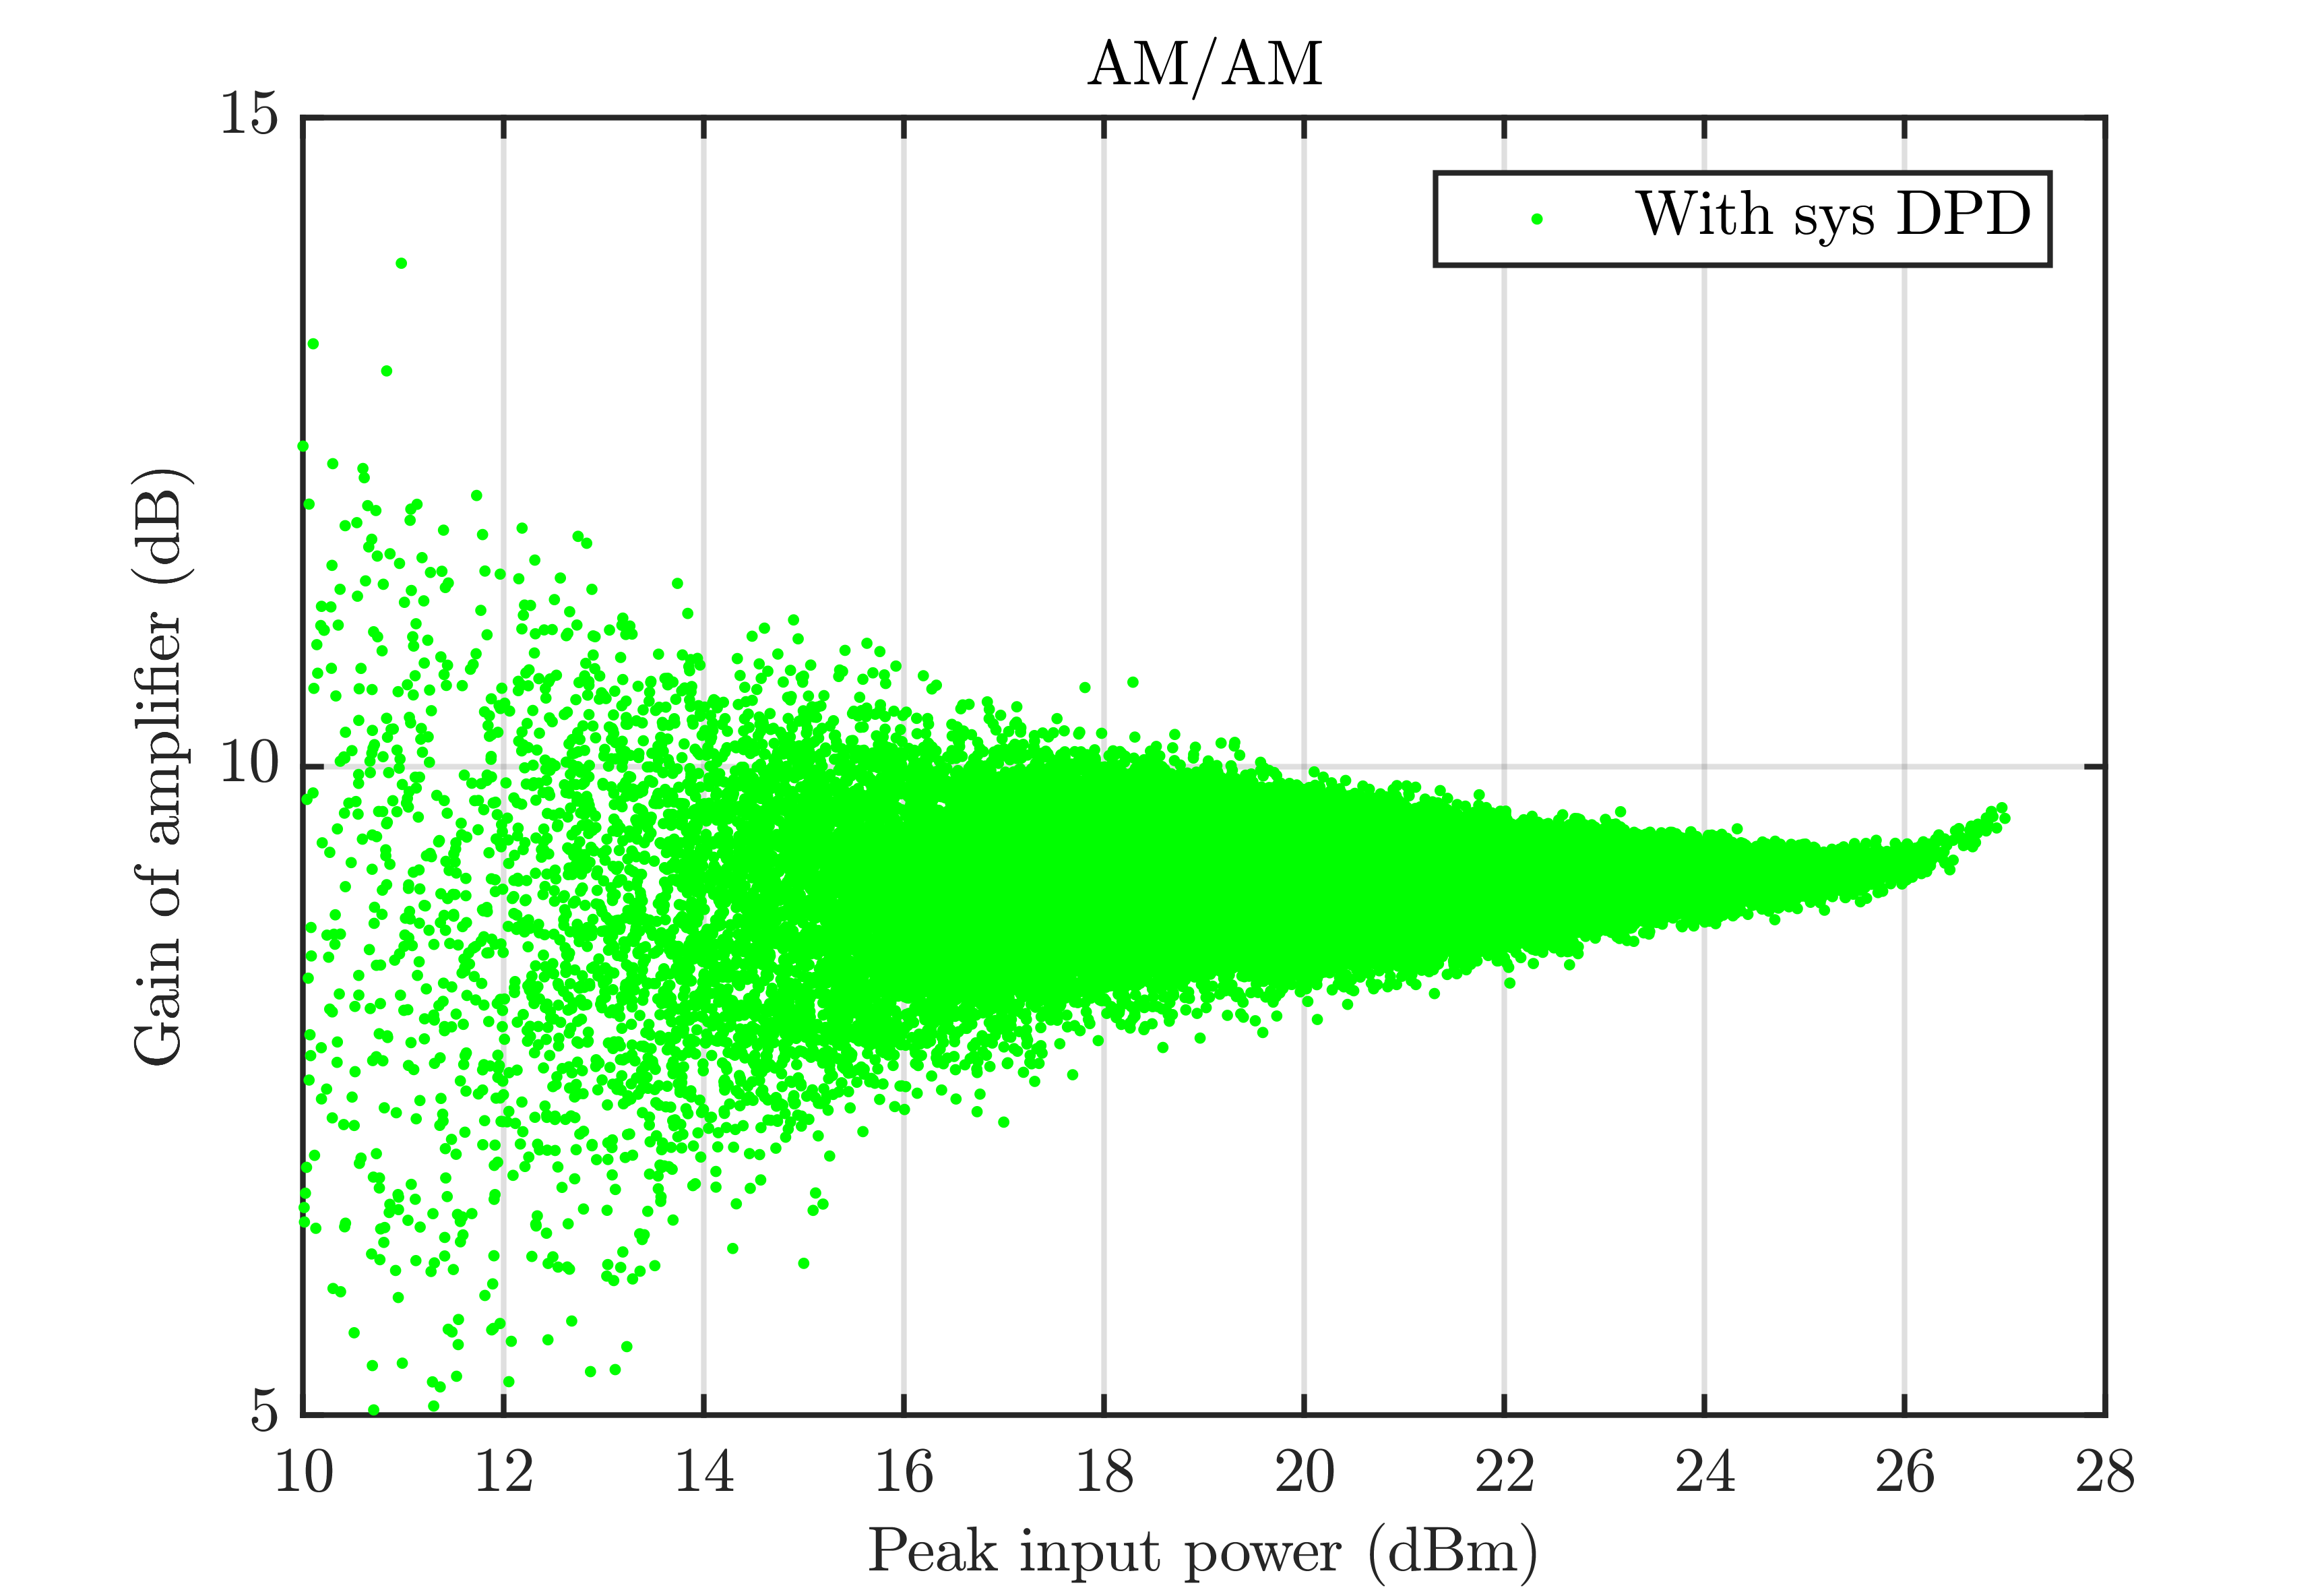
\includegraphics[scale = 0.5]{figures/measurement/cree/meas3/amam_sys_dpd_0p1.png}
	\caption{AM/AM distortion at $d = 0.1\lambda$ with system DPD}
    \label{fig:meas4_amam2}
  \end{minipage}
\end{figure}

\begin{figure}[H]
  \centering
  \begin{minipage}[b]{0.5\textwidth}
	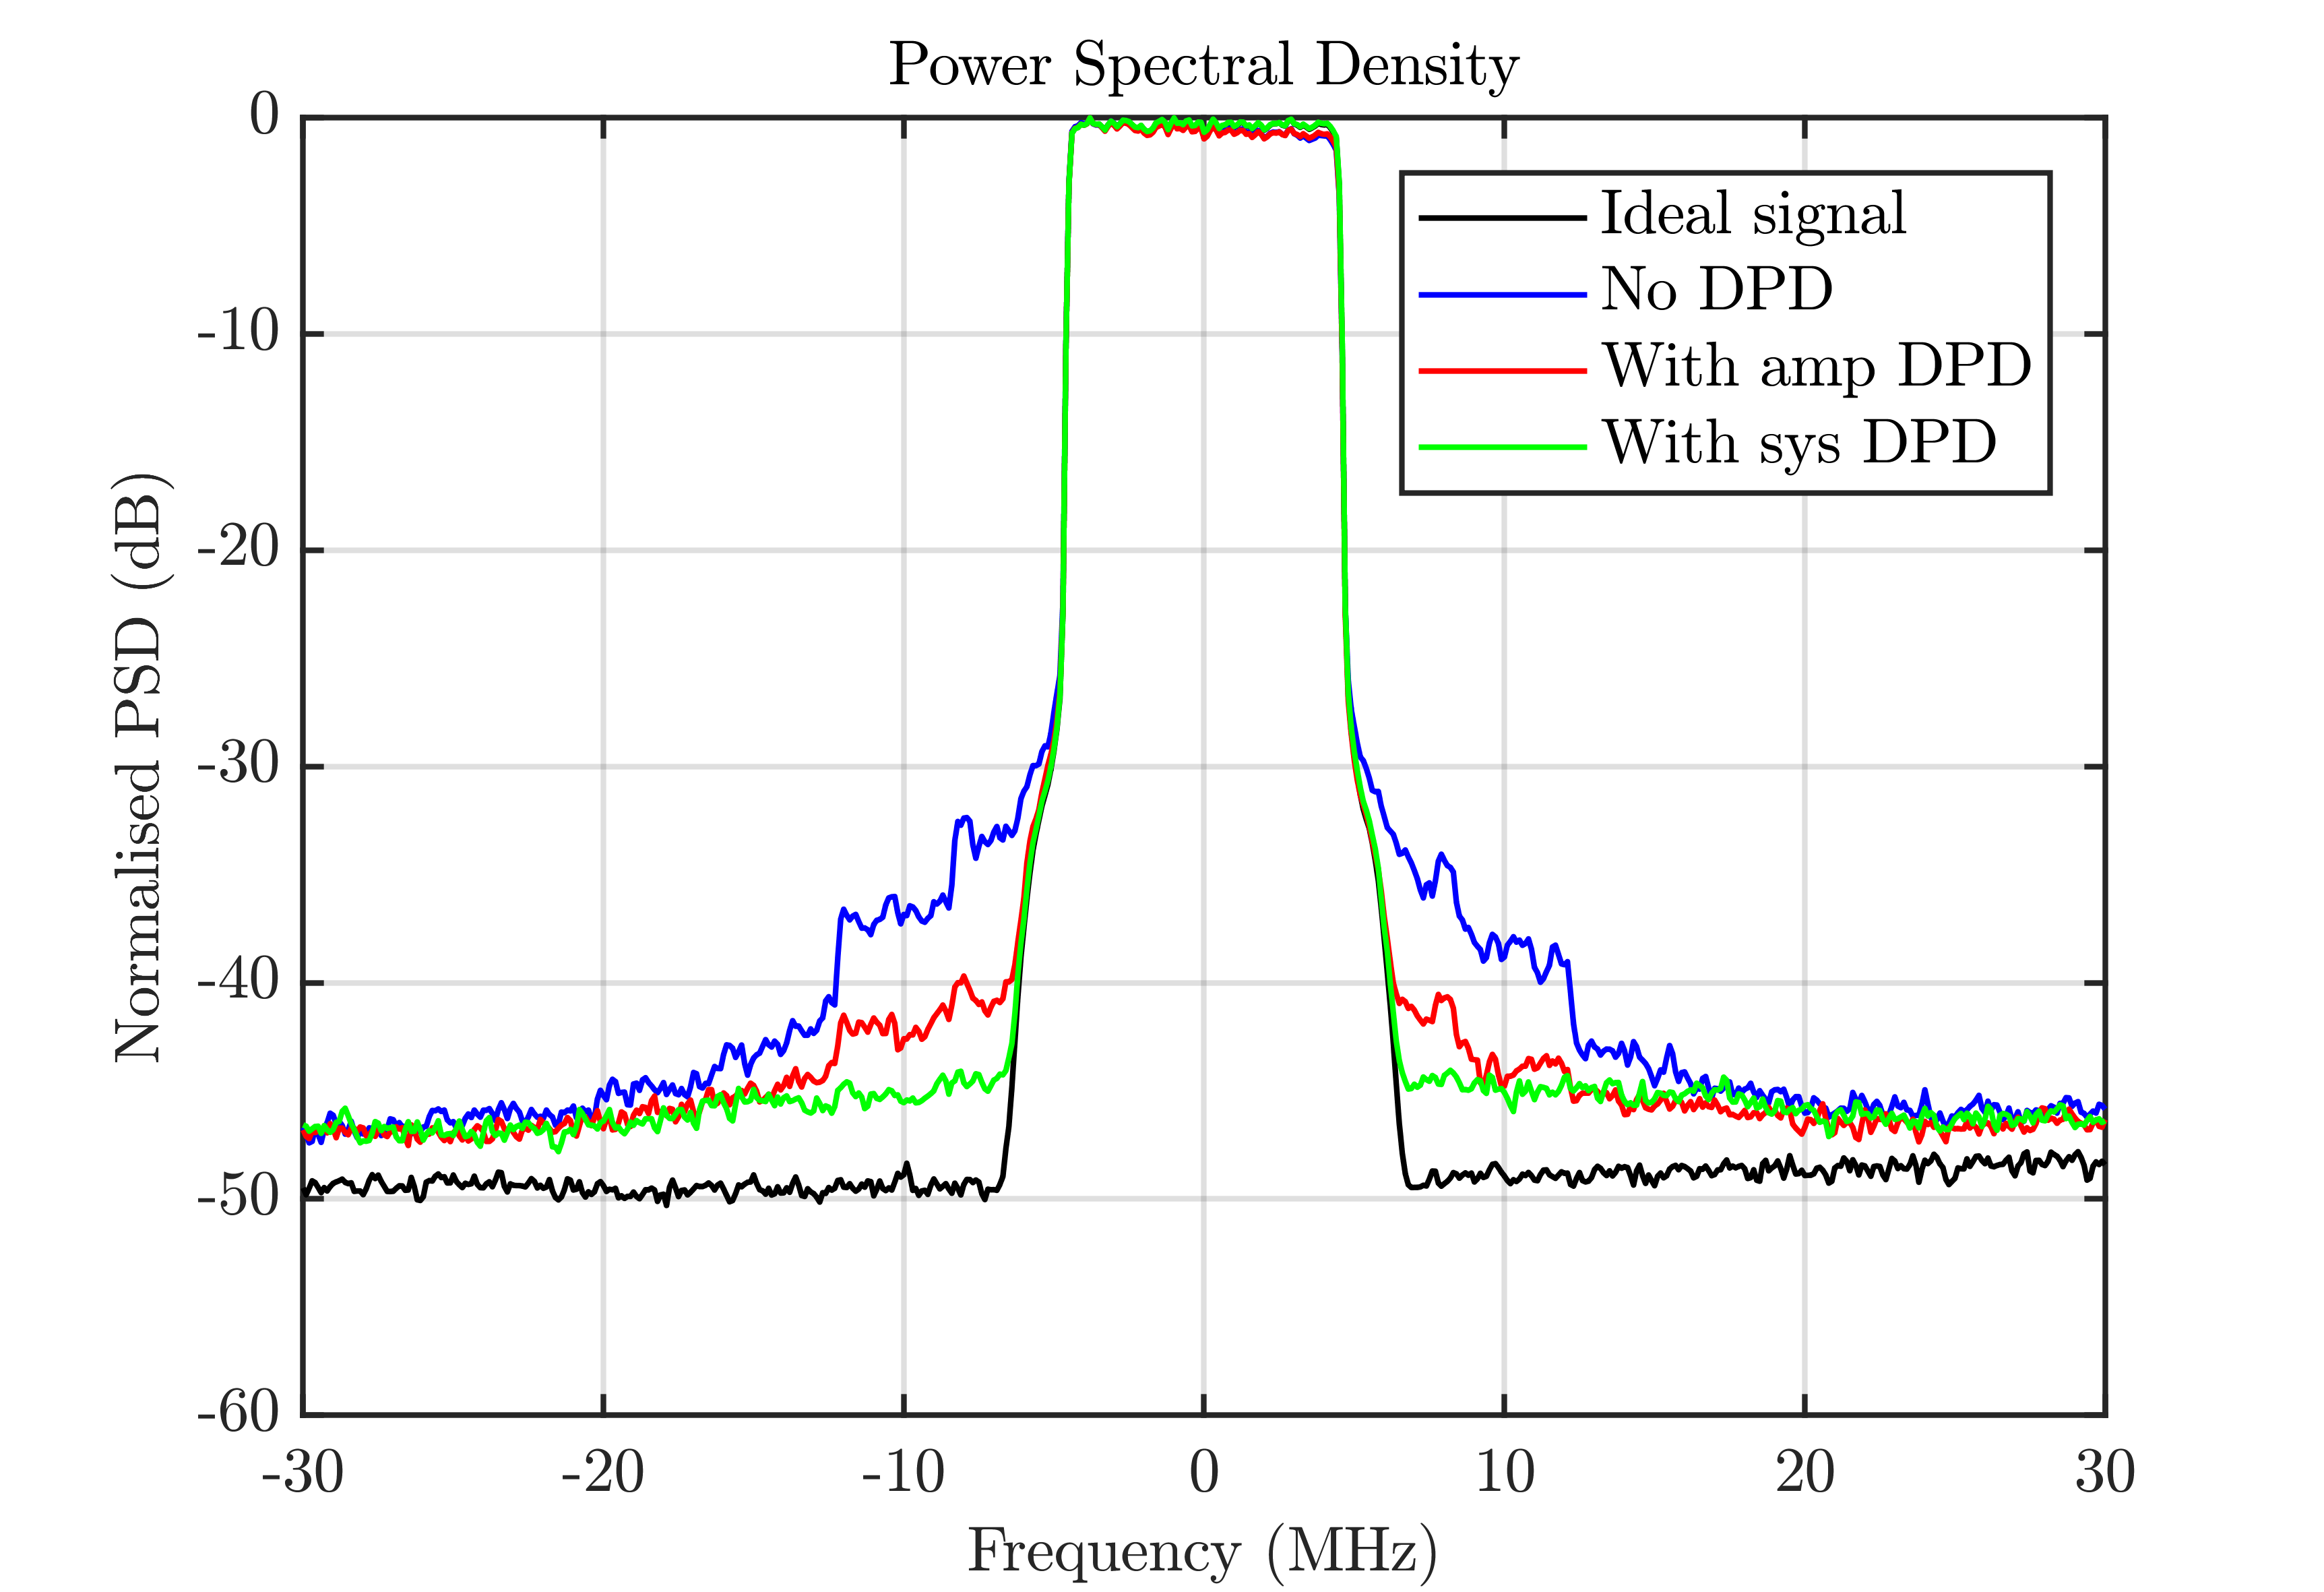
\includegraphics[scale = 0.5]{figures/measurement/cree/meas3/psd_0p1.png}
	\caption{PSD of measurement at $d = 0.1\lambda$ }	
    \label{fig:meas4_psd1}
  \end{minipage}
  \hfill
  \begin{minipage}[b]{0.4\textwidth}
	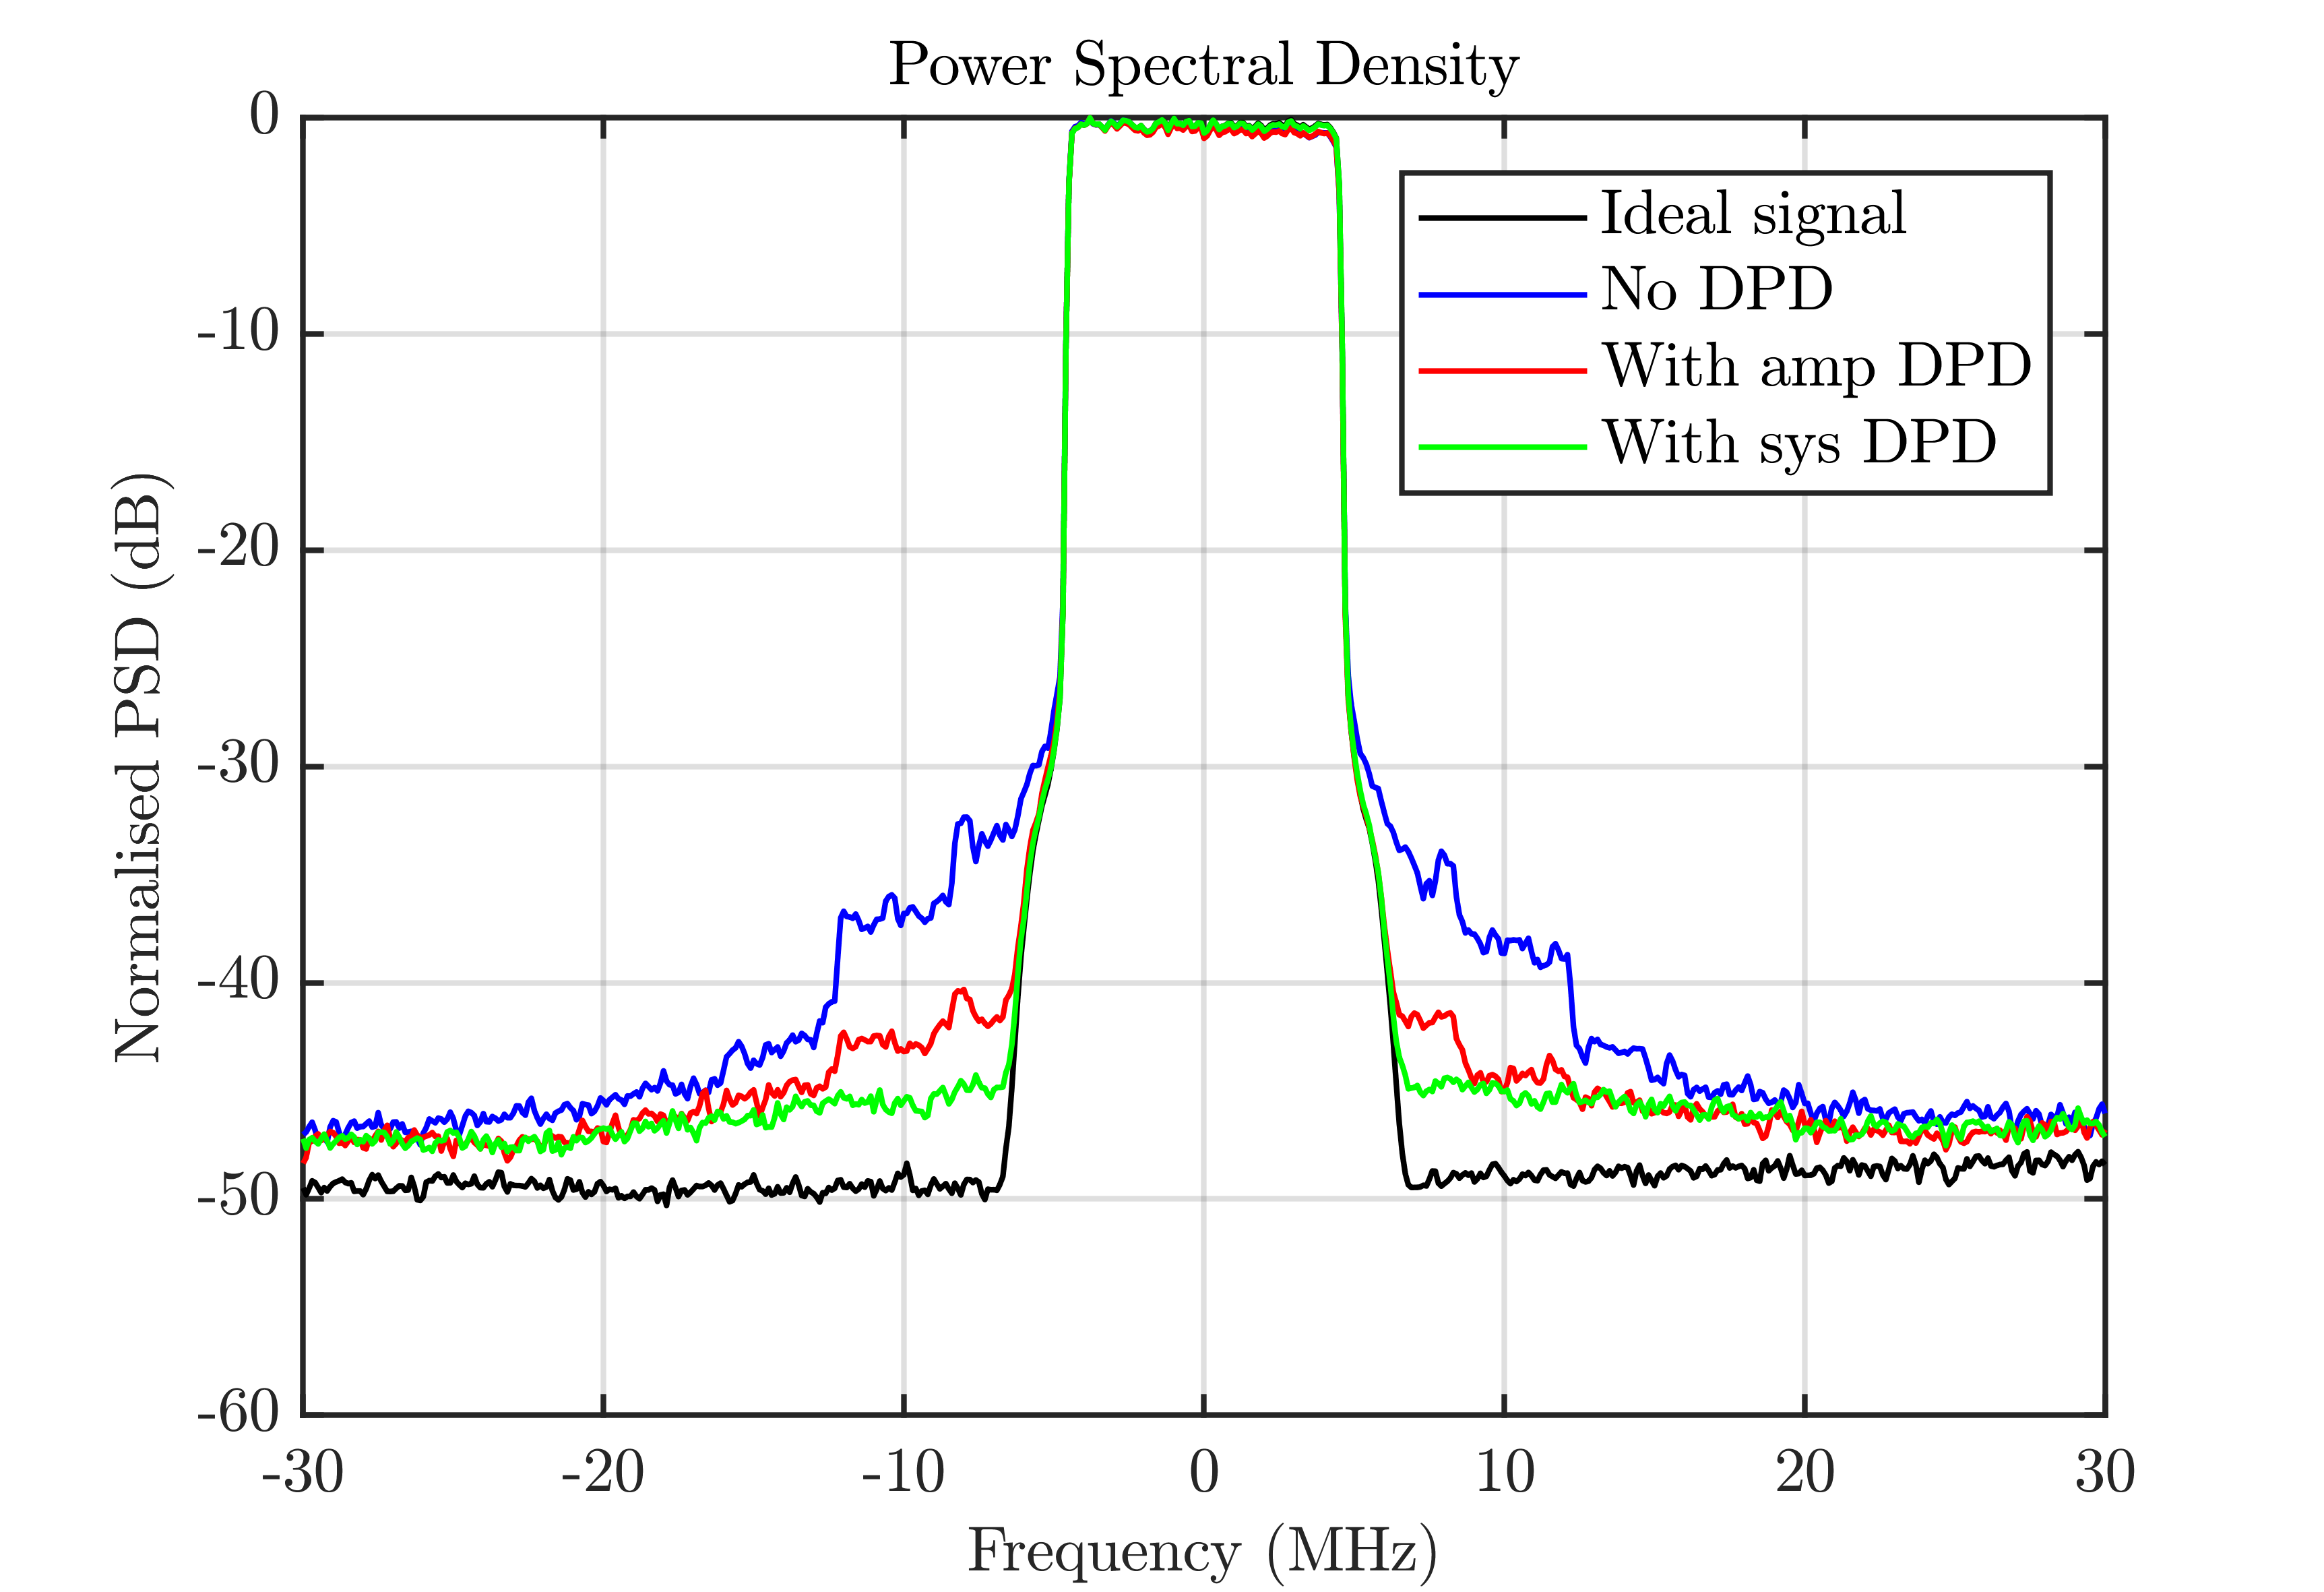
\includegraphics[scale = 0.5]{figures/measurement/cree/meas3/psd_0p2.png}
	\caption{PSD of measurement at $d = 0.2\lambda$}
    \label{fig:meas4_psd2}
  \end{minipage}
\end{figure}

\begin{figure}[H]
  \centering
  \begin{minipage}[b]{0.5\textwidth}
	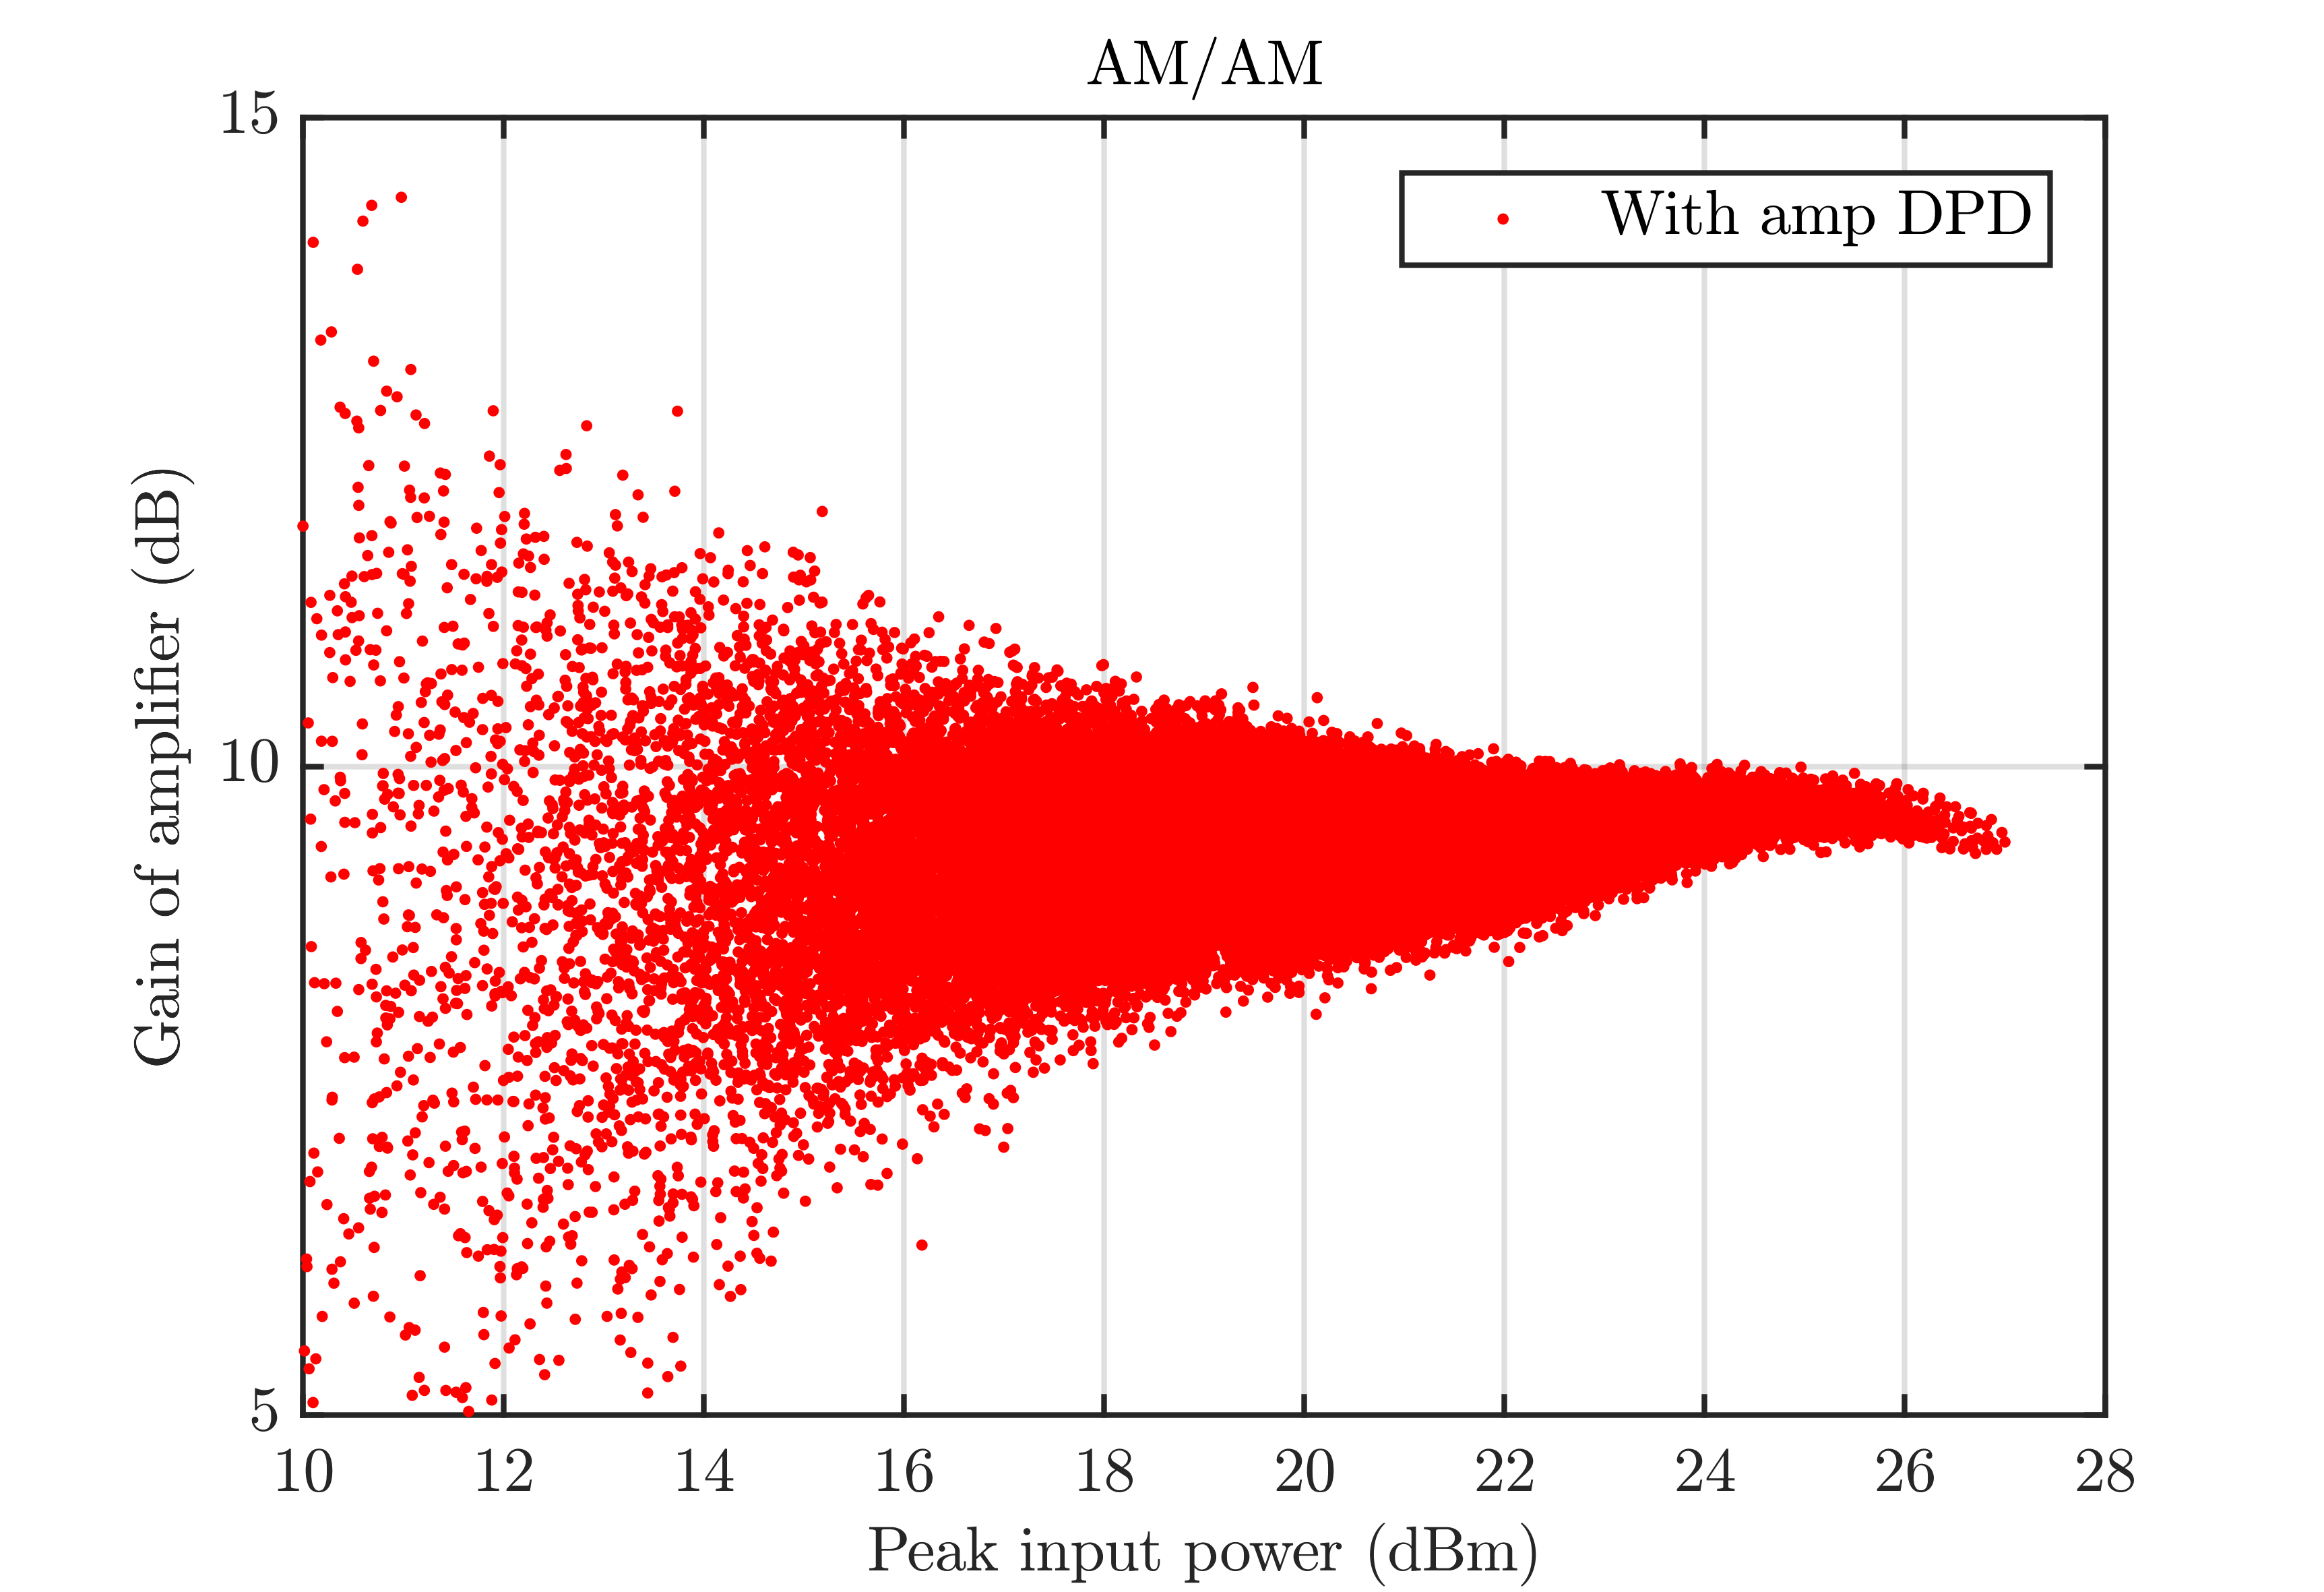
\includegraphics[scale = 0.5]{figures/measurement/cree/meas3/amam_amp_dpd_0p2.png}
	\caption{AM/AM distortion at $d = 0.2\lambda$ with amplifier DPD}	
    \label{fig:meas4_amam3}
  \end{minipage}
  \hfill
  \begin{minipage}[b]{0.4\textwidth}
	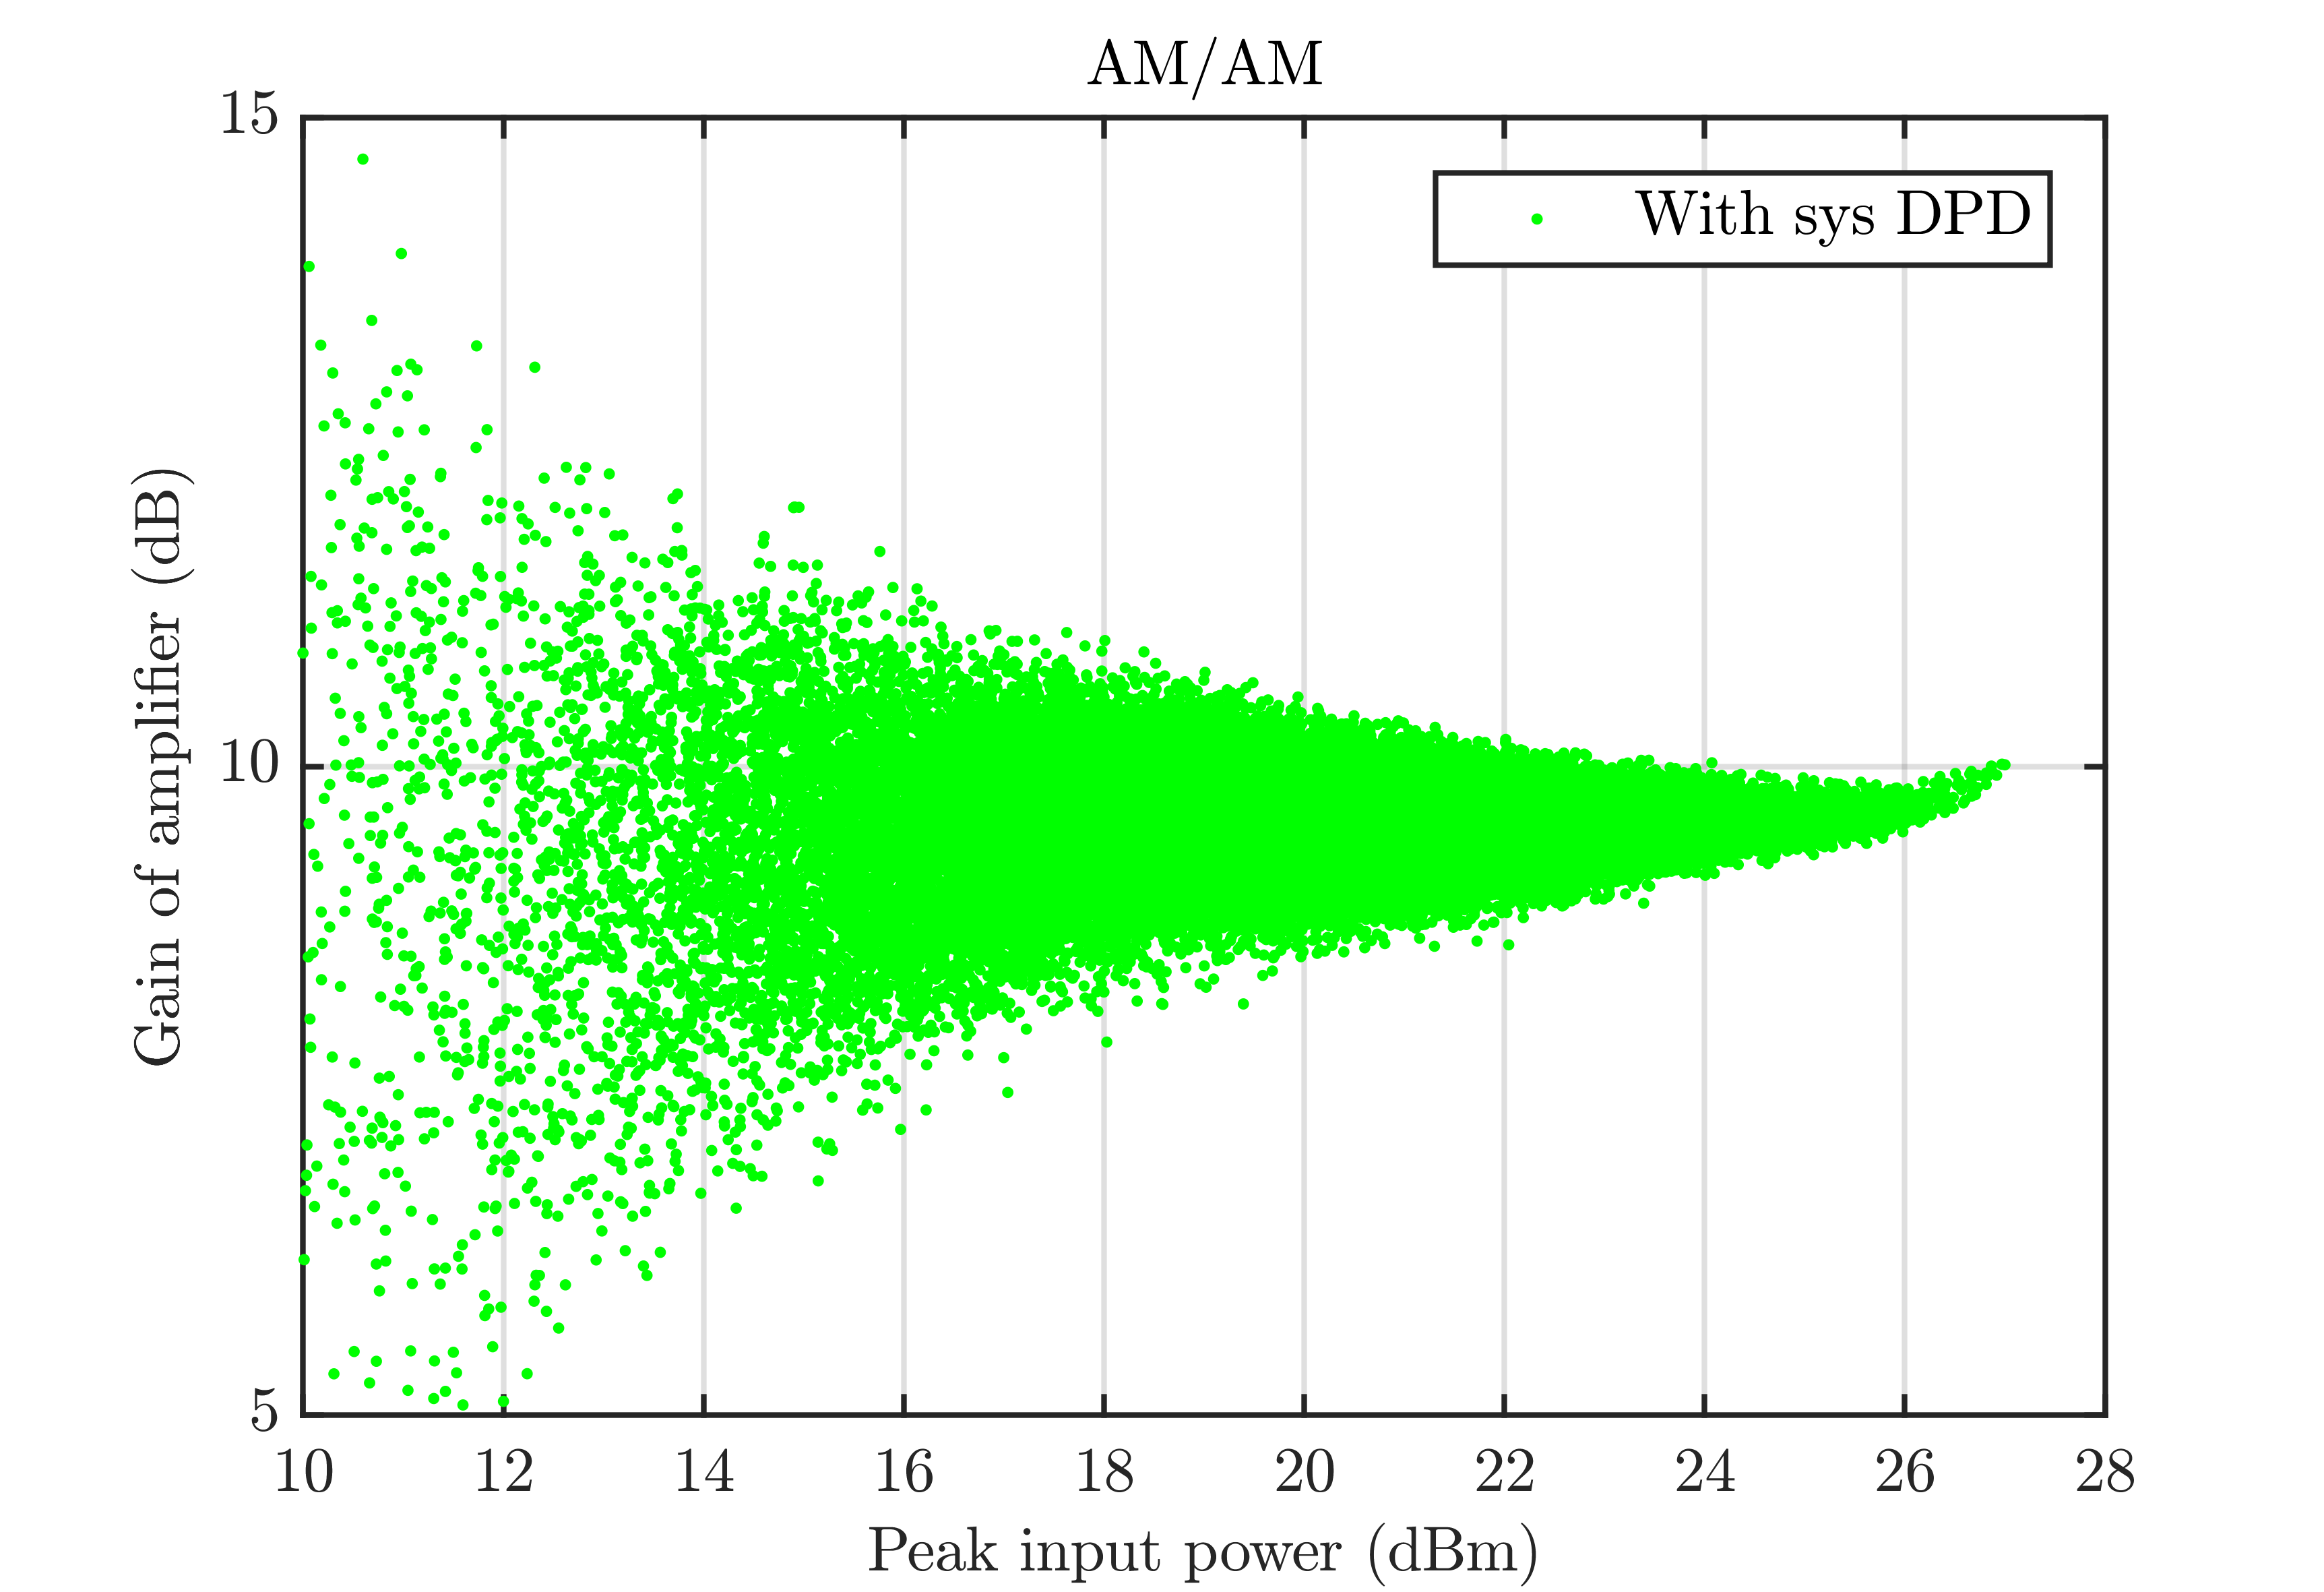
\includegraphics[scale = 0.5]{figures/measurement/cree/meas3/amam_sys_dpd_0p2.png}
	\caption{AM/AM distortion at $d = 0.2\lambda$ with system DPD}
    \label{fig:meas4_amam4}
  \end{minipage}
\end{figure}

\begin{figure}[H]
  \centering
  \begin{minipage}[b]{0.5\textwidth}
	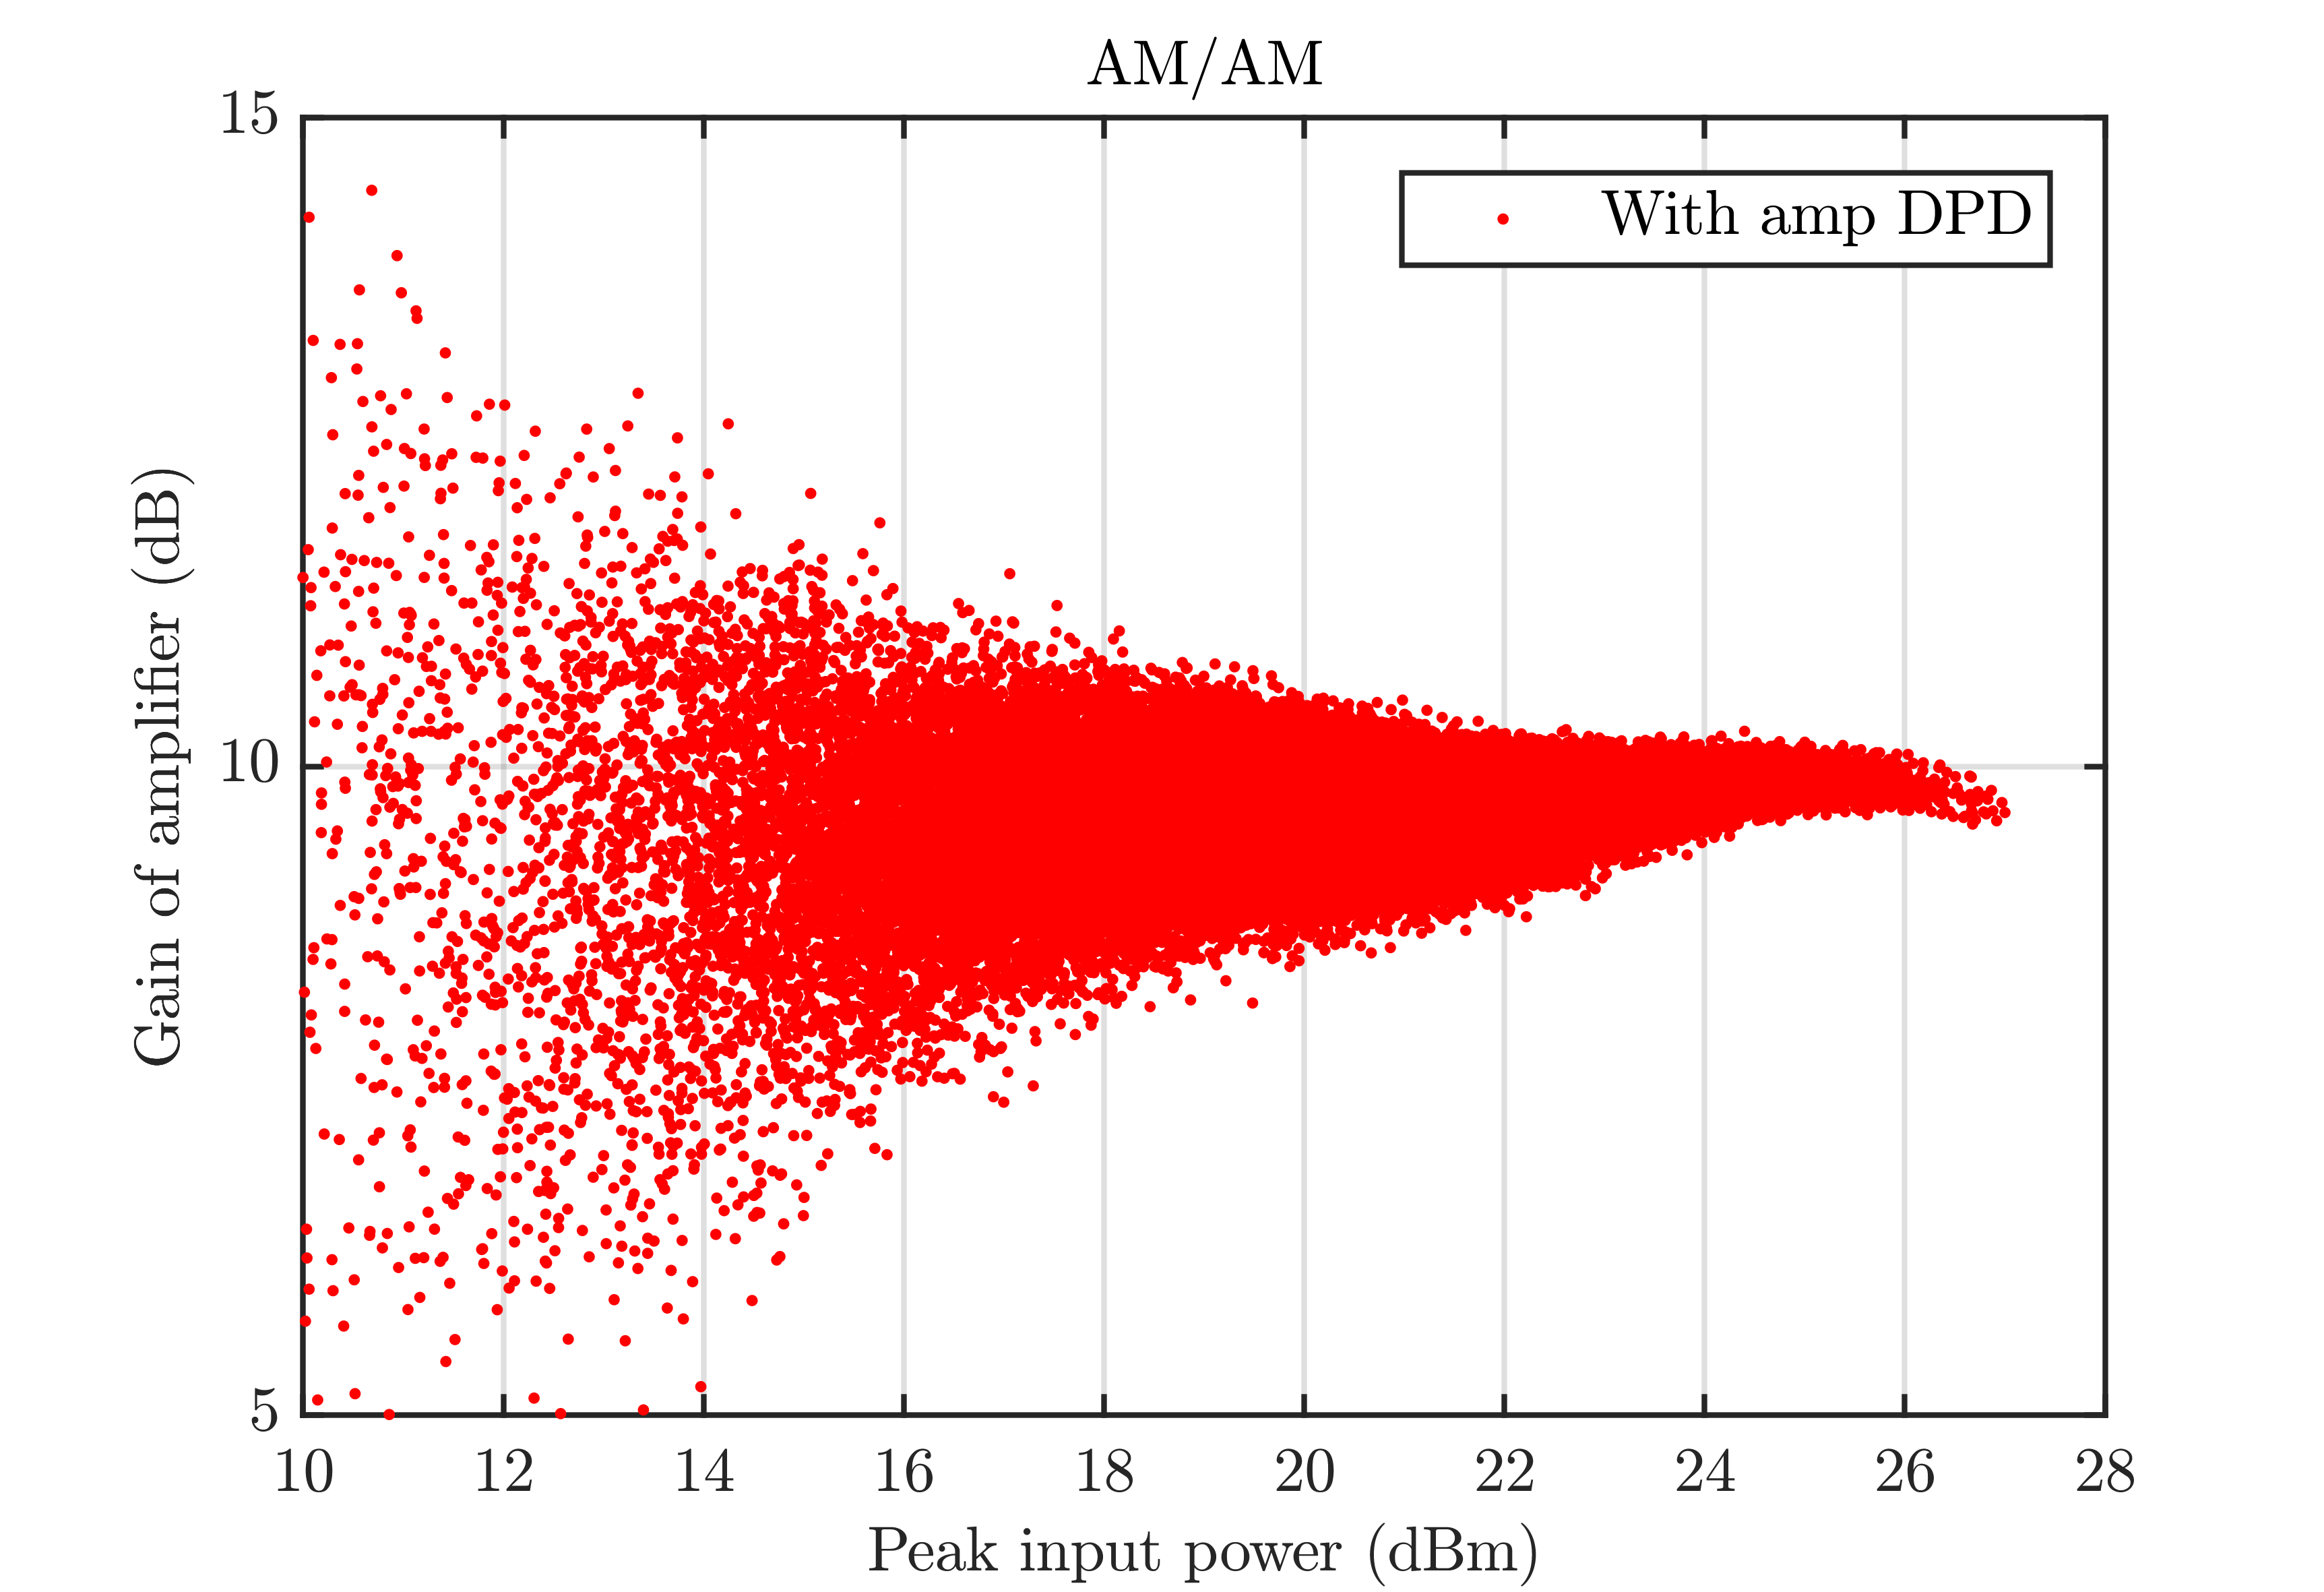
\includegraphics[scale = 0.5]{figures/measurement/cree/meas3/amam_amp_dpd_0p3.png}
	\caption{AM/AM distortion at $d = 0.3\lambda$ with amplifier DPD}	
    \label{fig:meas4_amam5}
  \end{minipage}
  \hfill
  \begin{minipage}[b]{0.4\textwidth}
	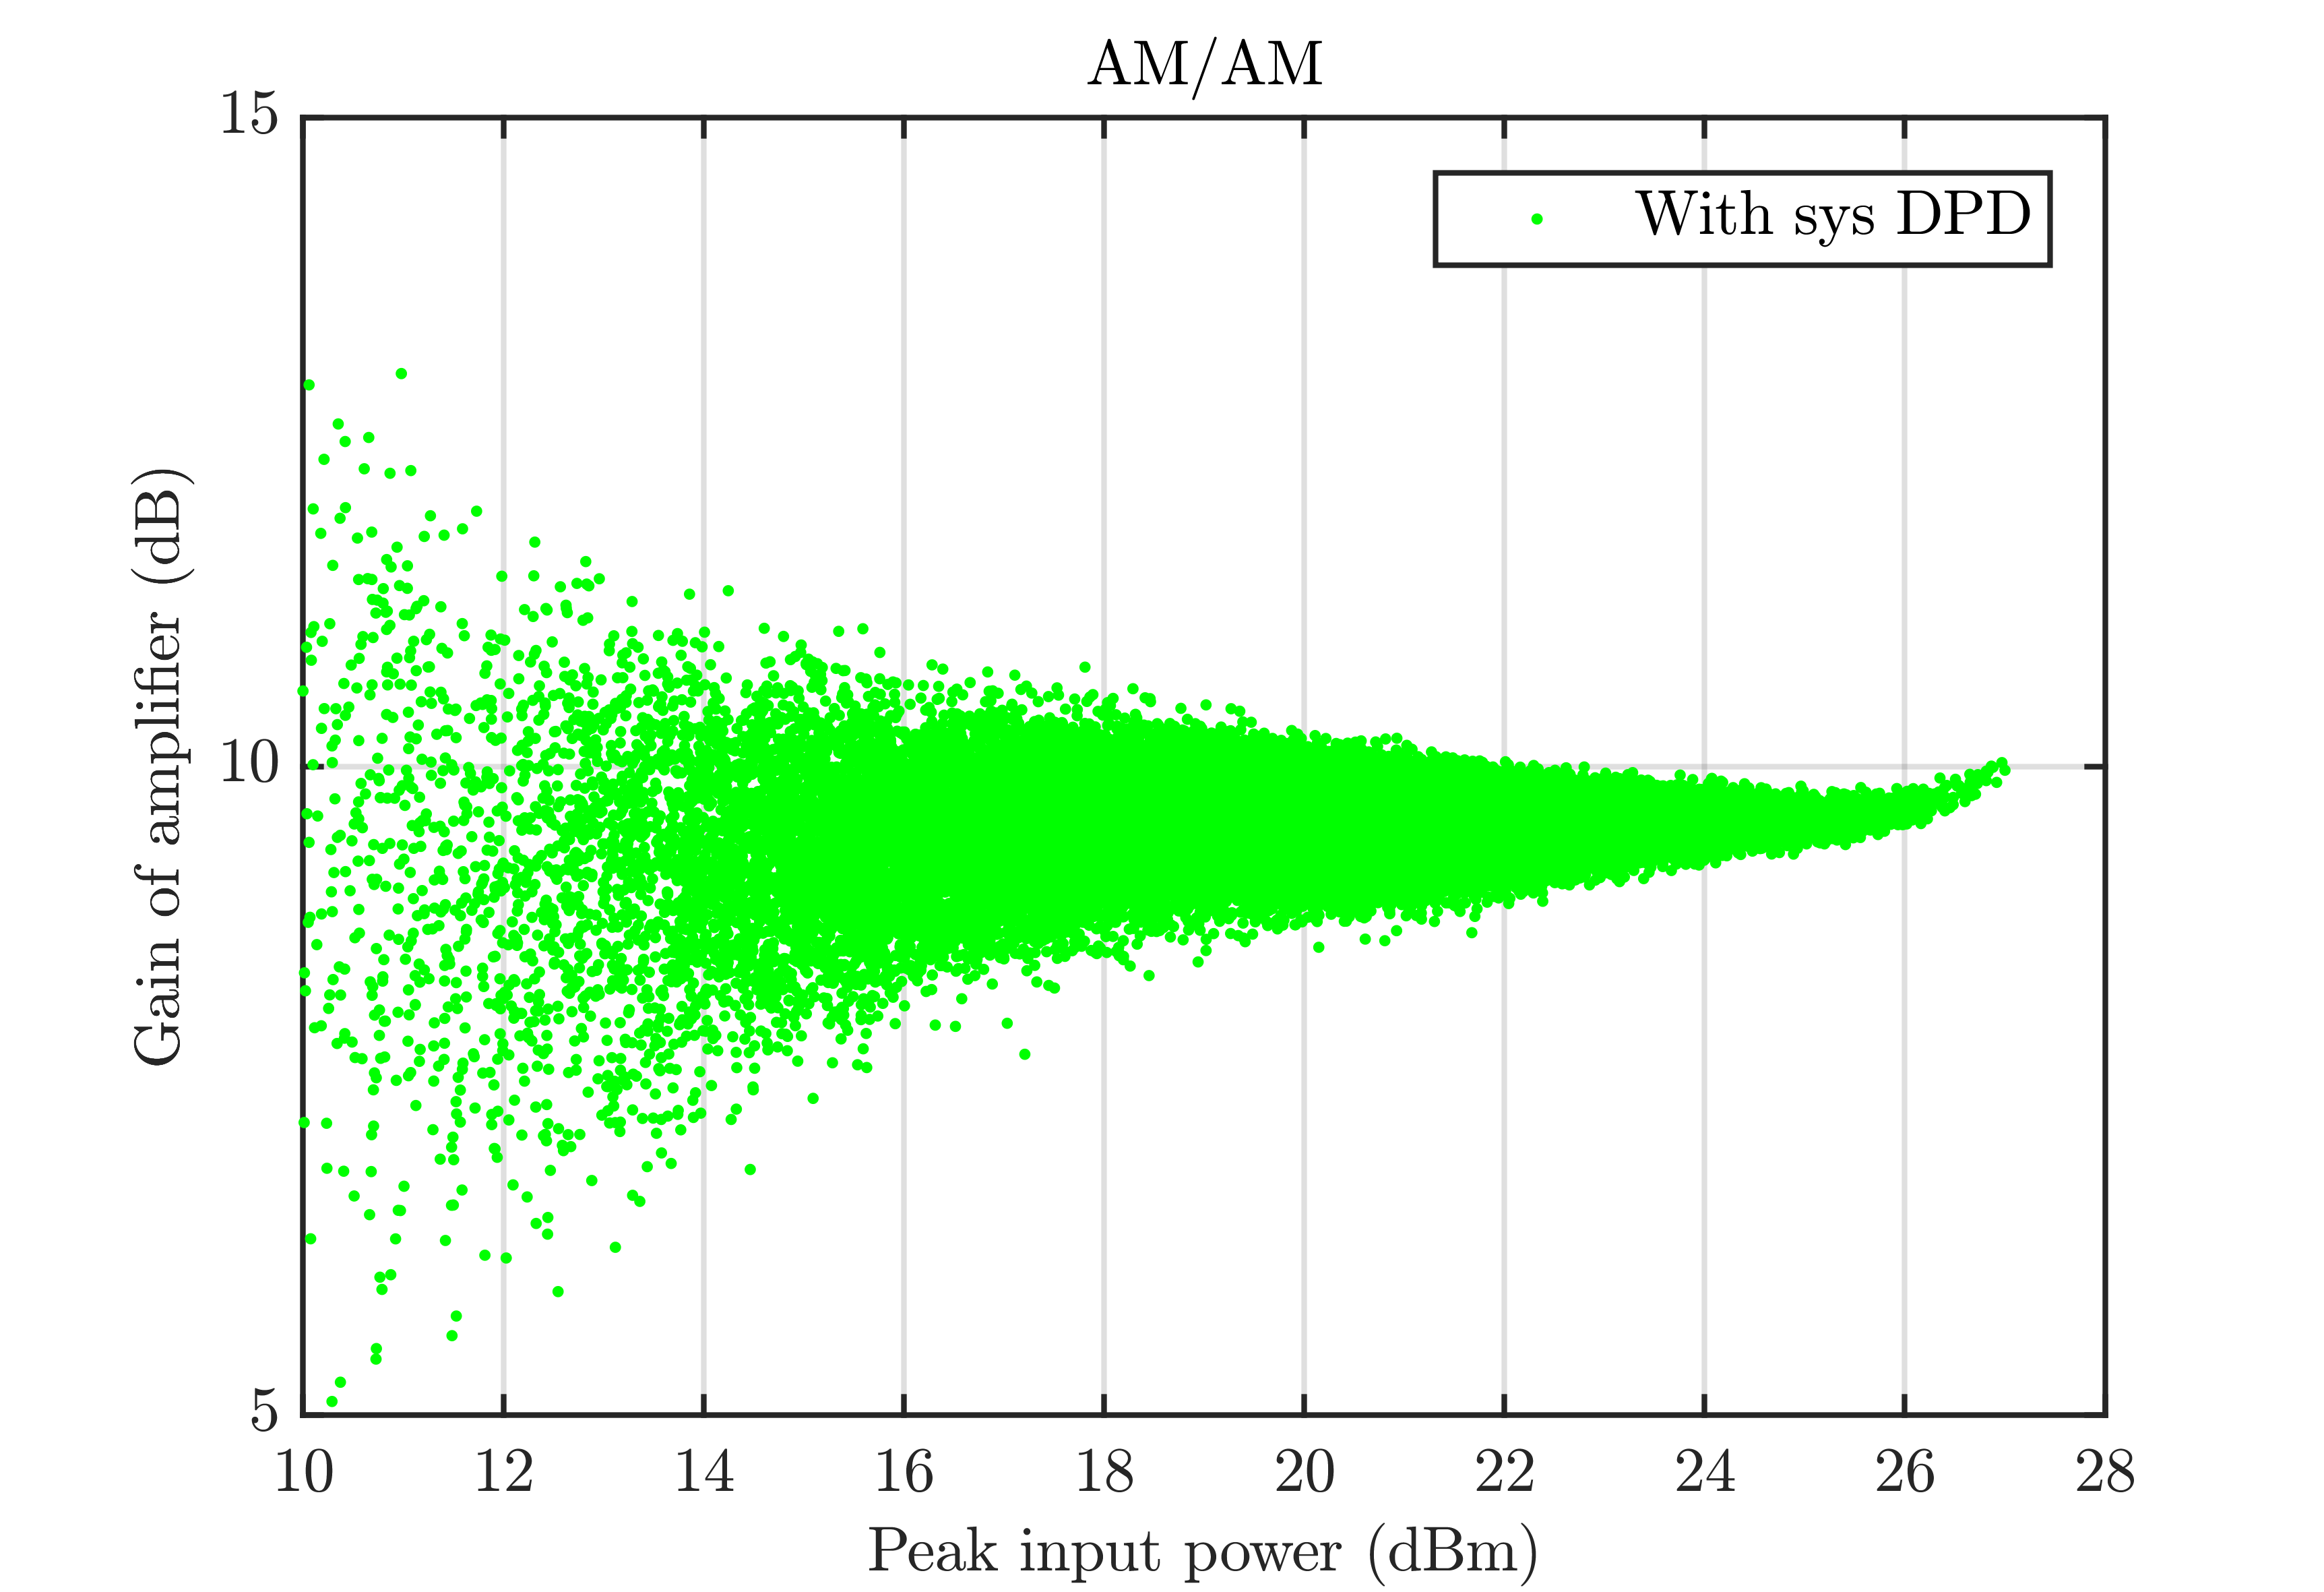
\includegraphics[scale = 0.5]{figures/measurement/cree/meas3/amam_sys_dpd_0p3.png}
	\caption{AM/AM distortion at $d = 0.3\lambda$ with system DPD}
    \label{fig:meas4_amam6}
  \end{minipage}
\end{figure}

\begin{figure}[H]
  \centering
  \begin{minipage}[b]{0.5\textwidth}
	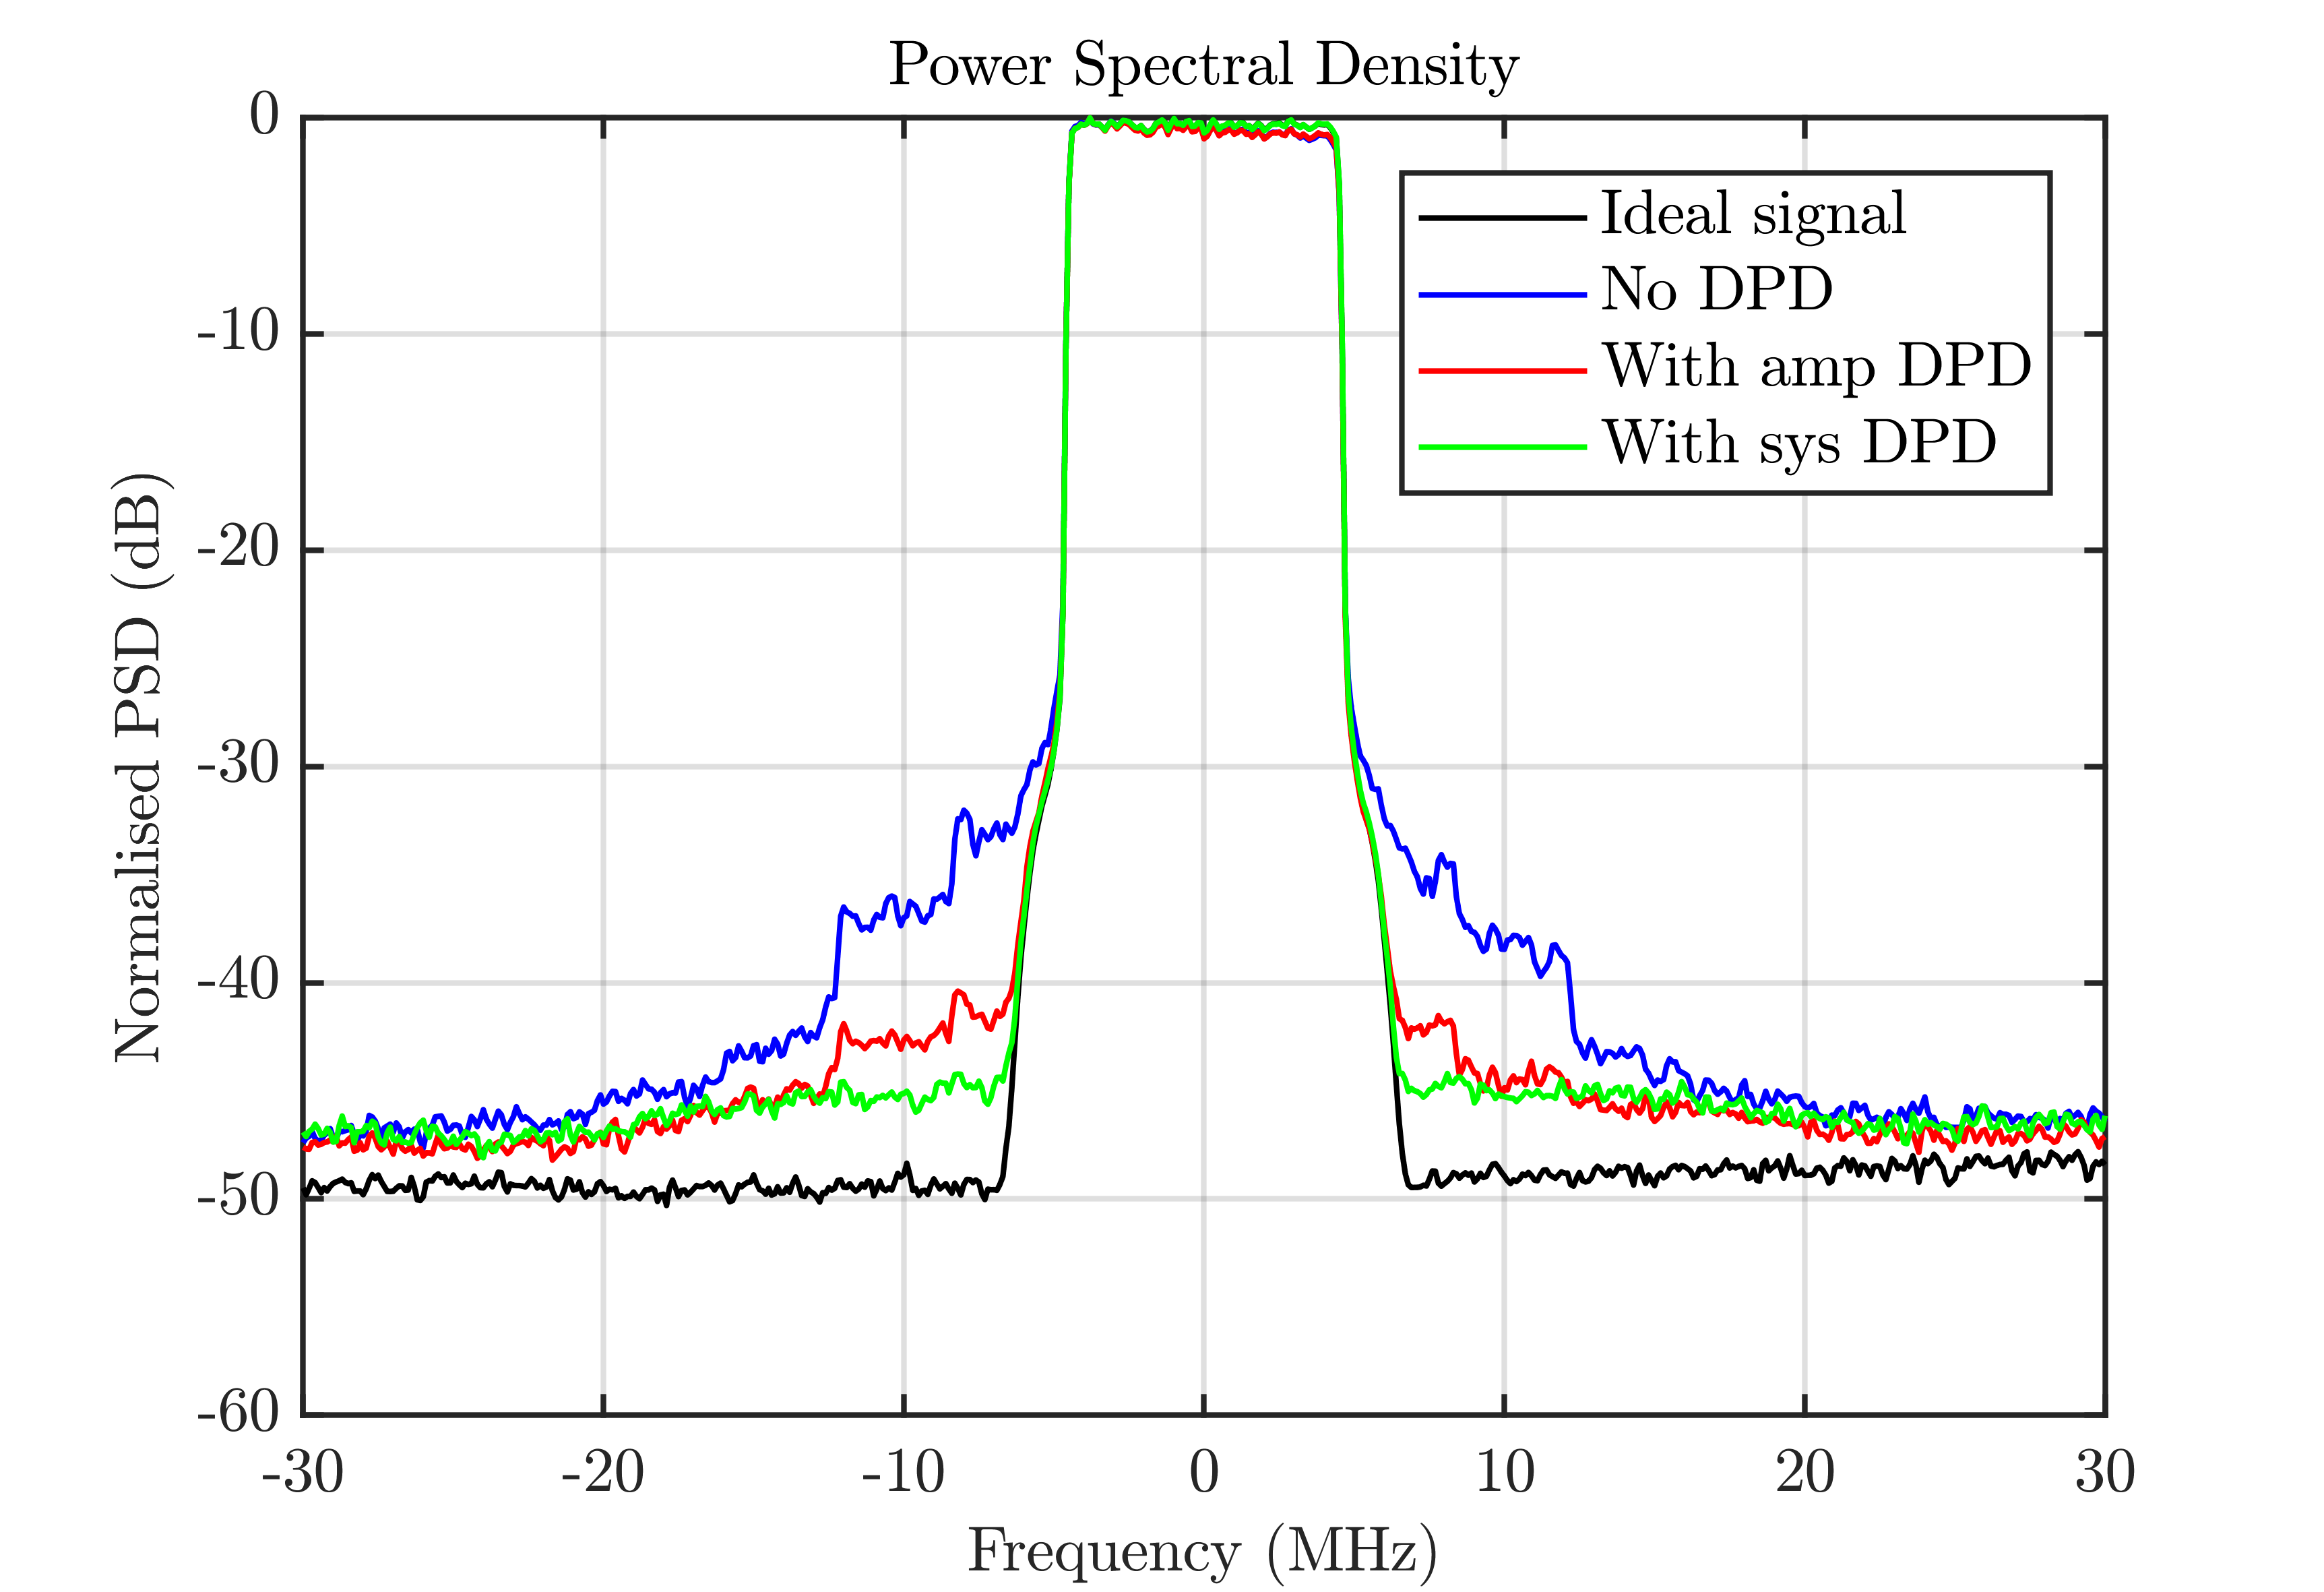
\includegraphics[scale = 0.5]{figures/measurement/cree/meas3/psd_0p3.png}
	\caption{PSD of measurement at $d = 0.3\lambda$ }	
    \label{fig:meas4_psd3}
  \end{minipage}
  \hfill
  \begin{minipage}[b]{0.4\textwidth}
	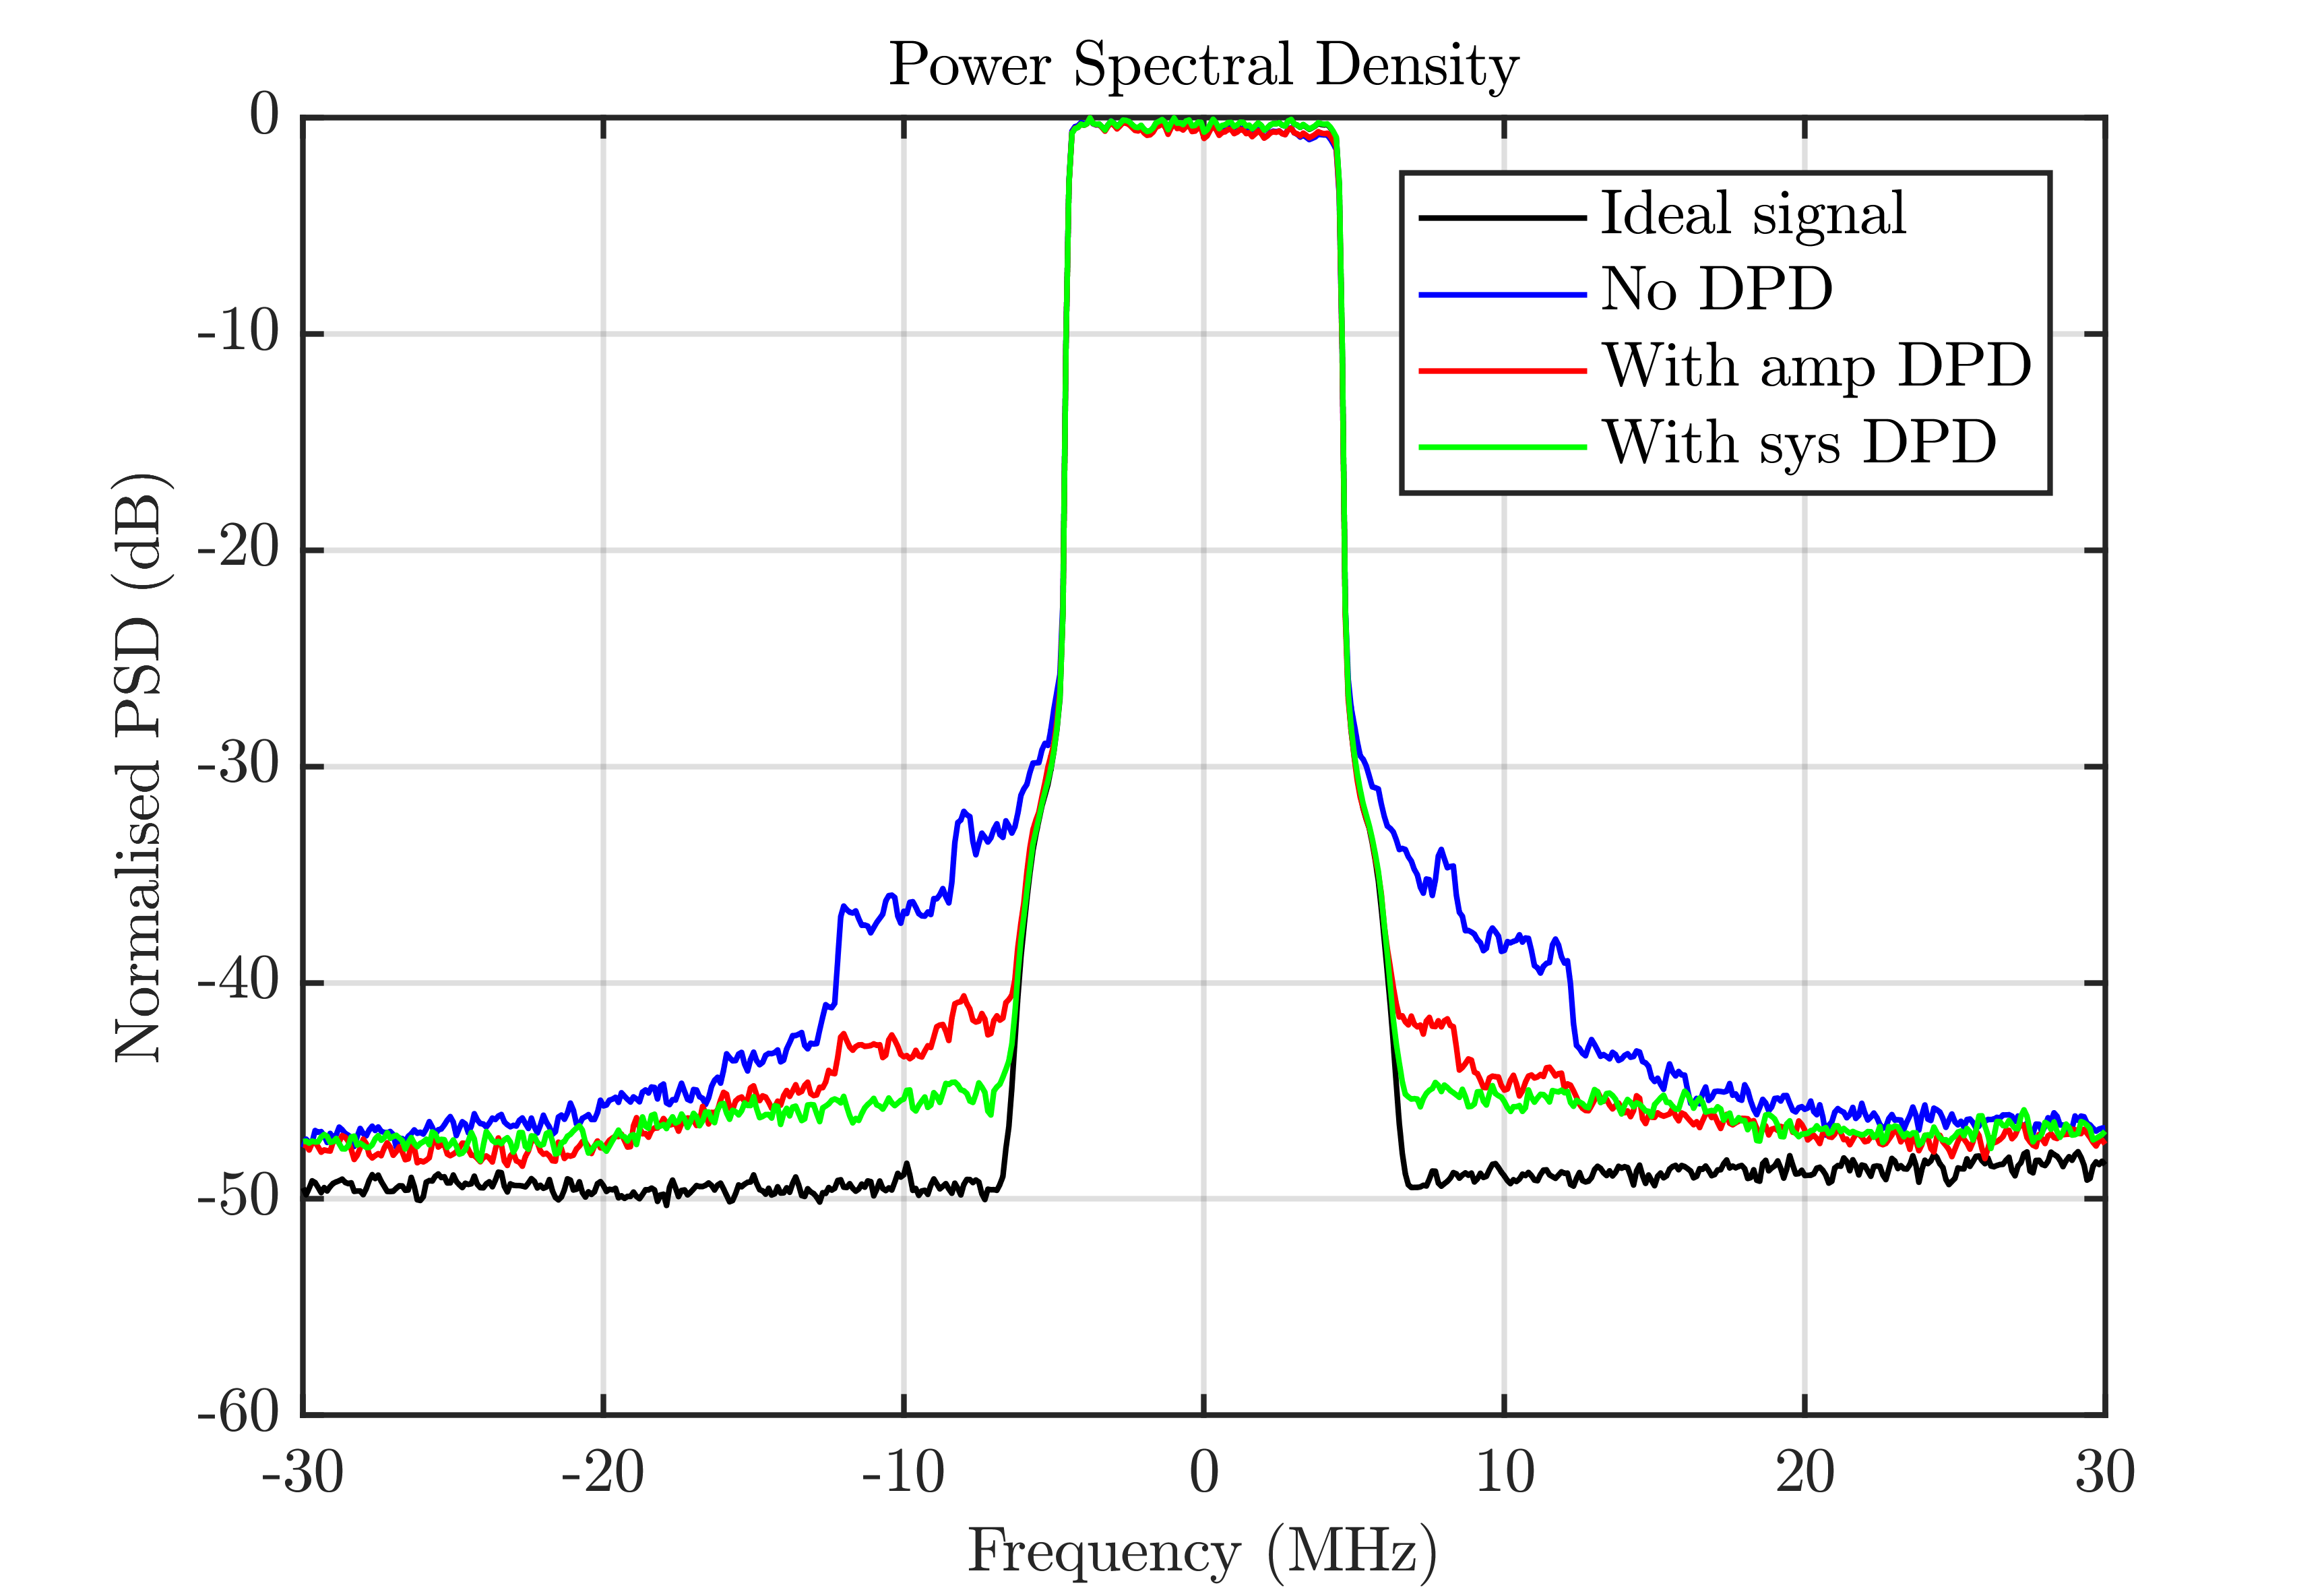
\includegraphics[scale = 0.5]{figures/measurement/cree/meas3/psd_0p4.png}
	\caption{PSD of measurement at $d = 0.4\lambda$}
    \label{fig:meas4_psd4}
  \end{minipage}
\end{figure}

\begin{figure}[H]
  \centering
  \begin{minipage}[b]{0.5\textwidth}
	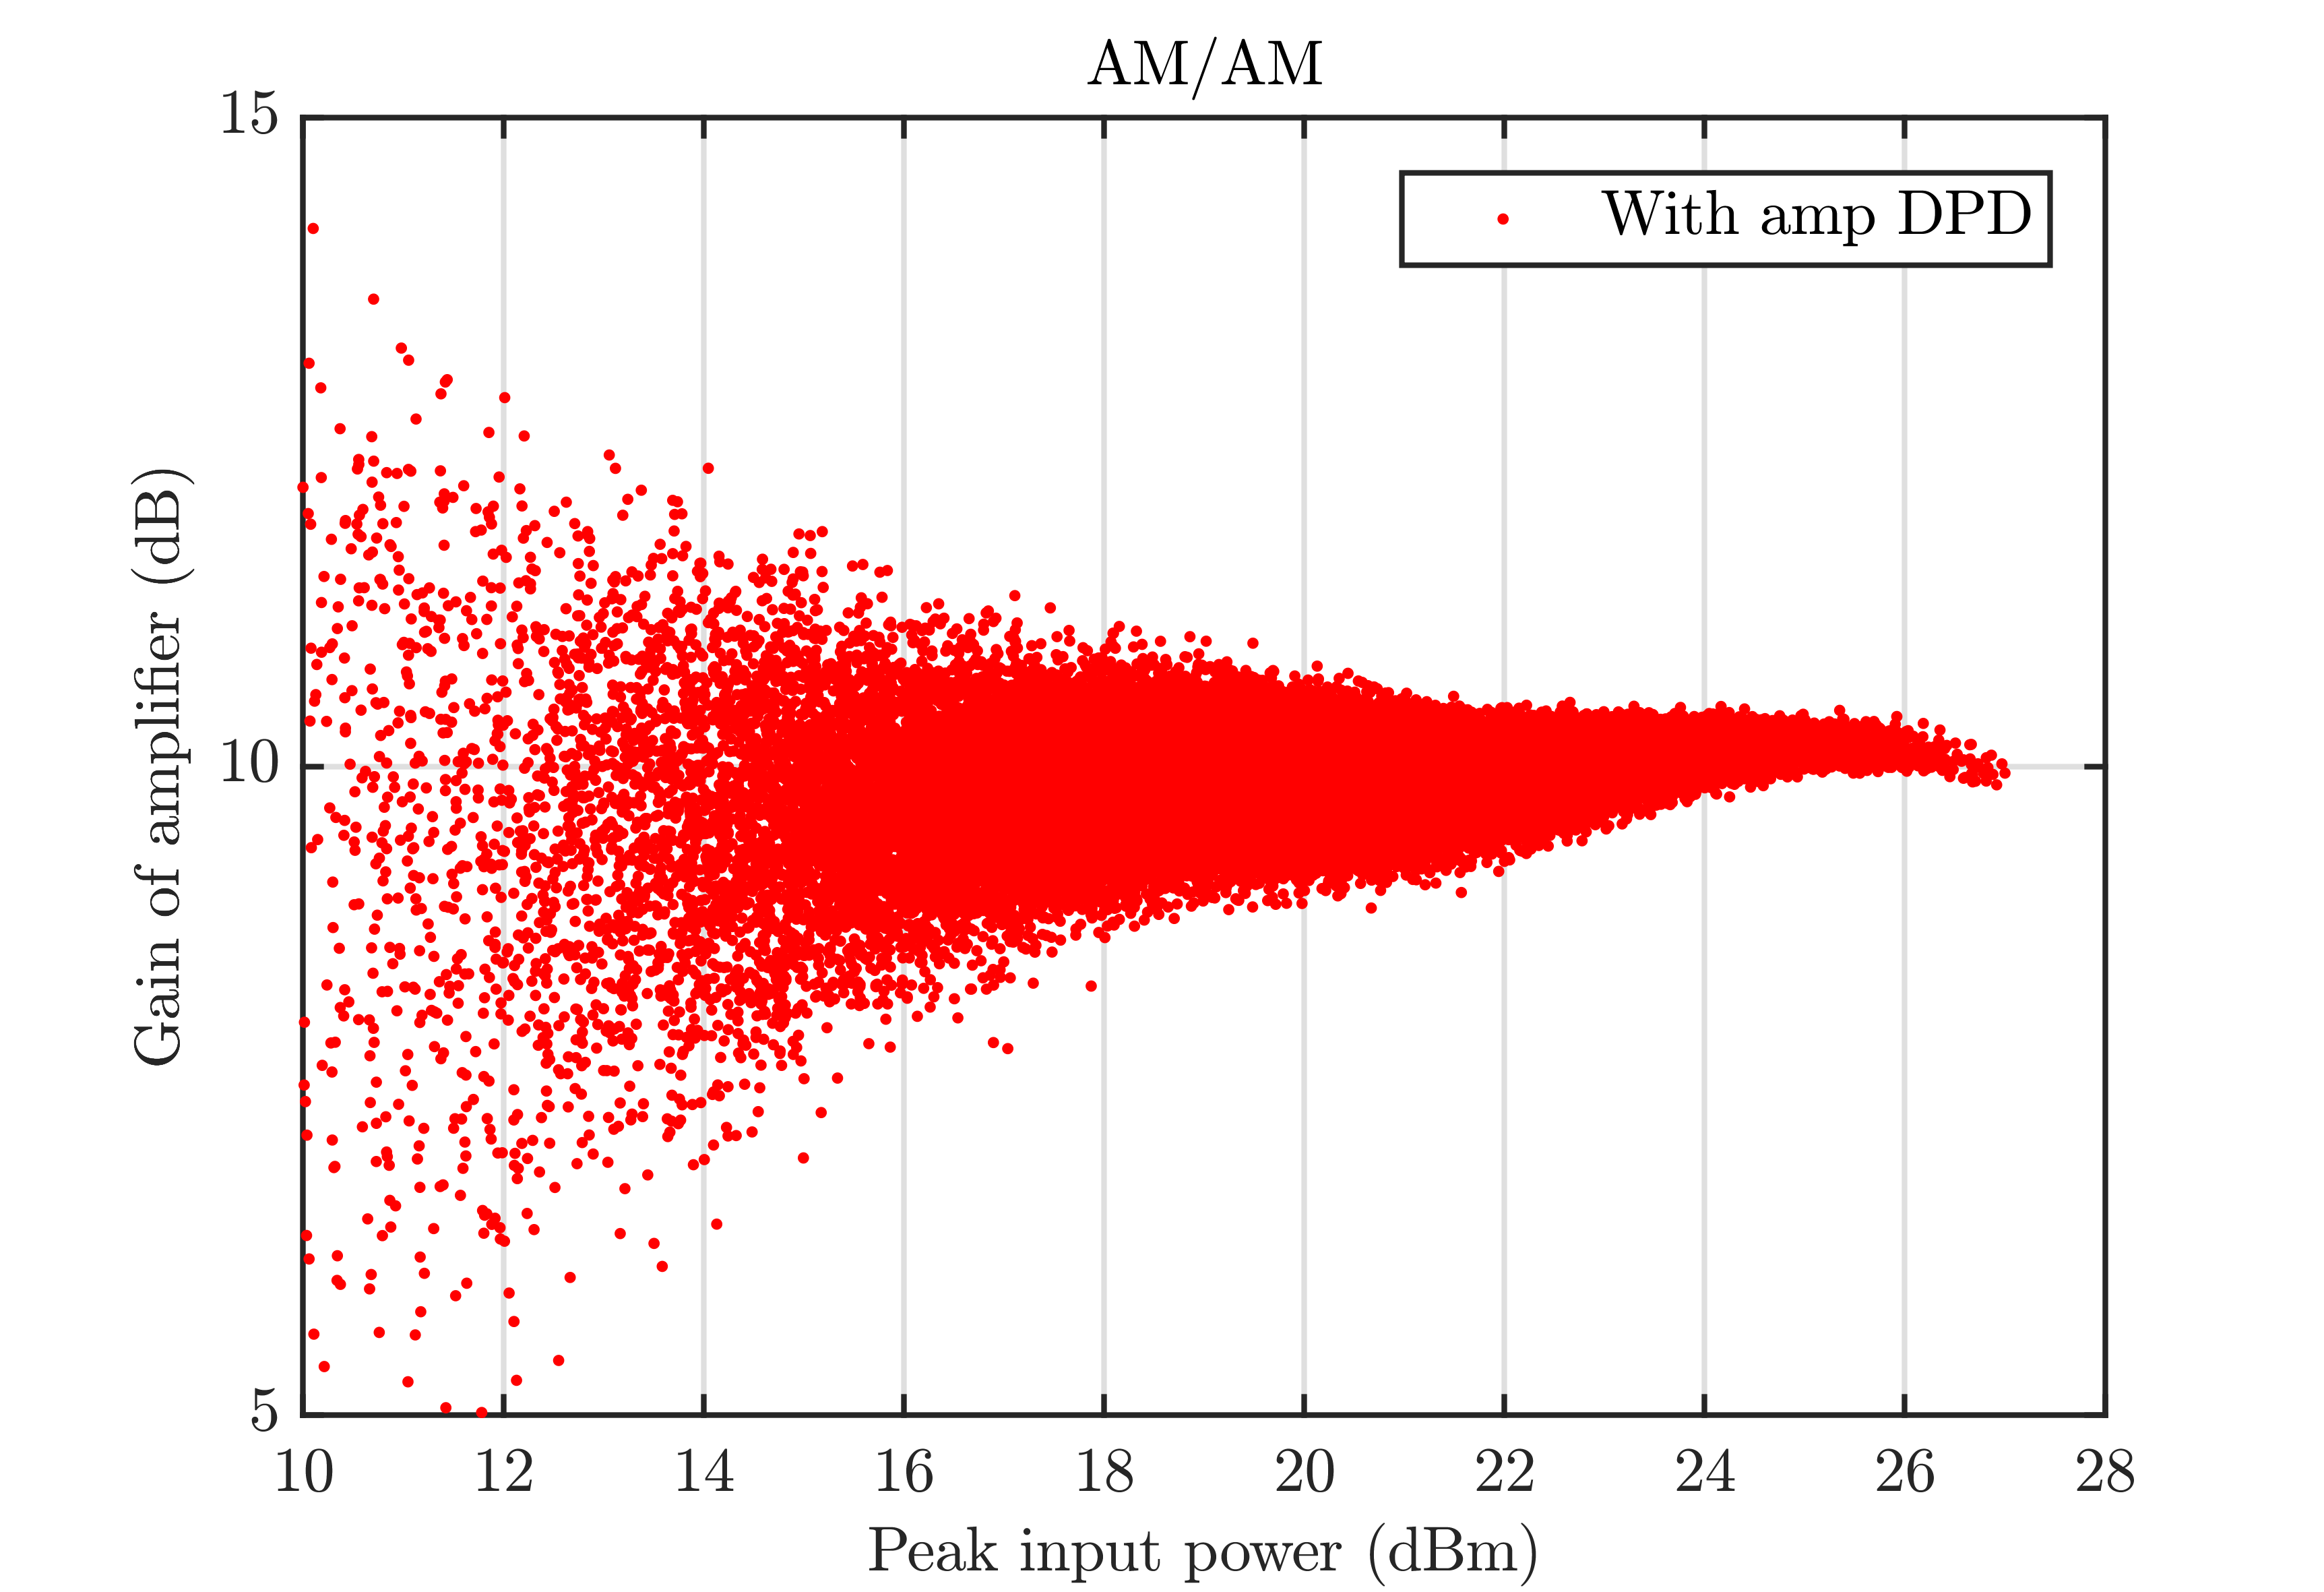
\includegraphics[scale = 0.5]{figures/measurement/cree/meas3/amam_amp_dpd_0p4.png}
	\caption{AM/AM distortion at $d = 0.4\lambda$ with amplifier DPD}	
    \label{fig:meas4_amam7}
  \end{minipage}
  \hfill
  \begin{minipage}[b]{0.4\textwidth}
	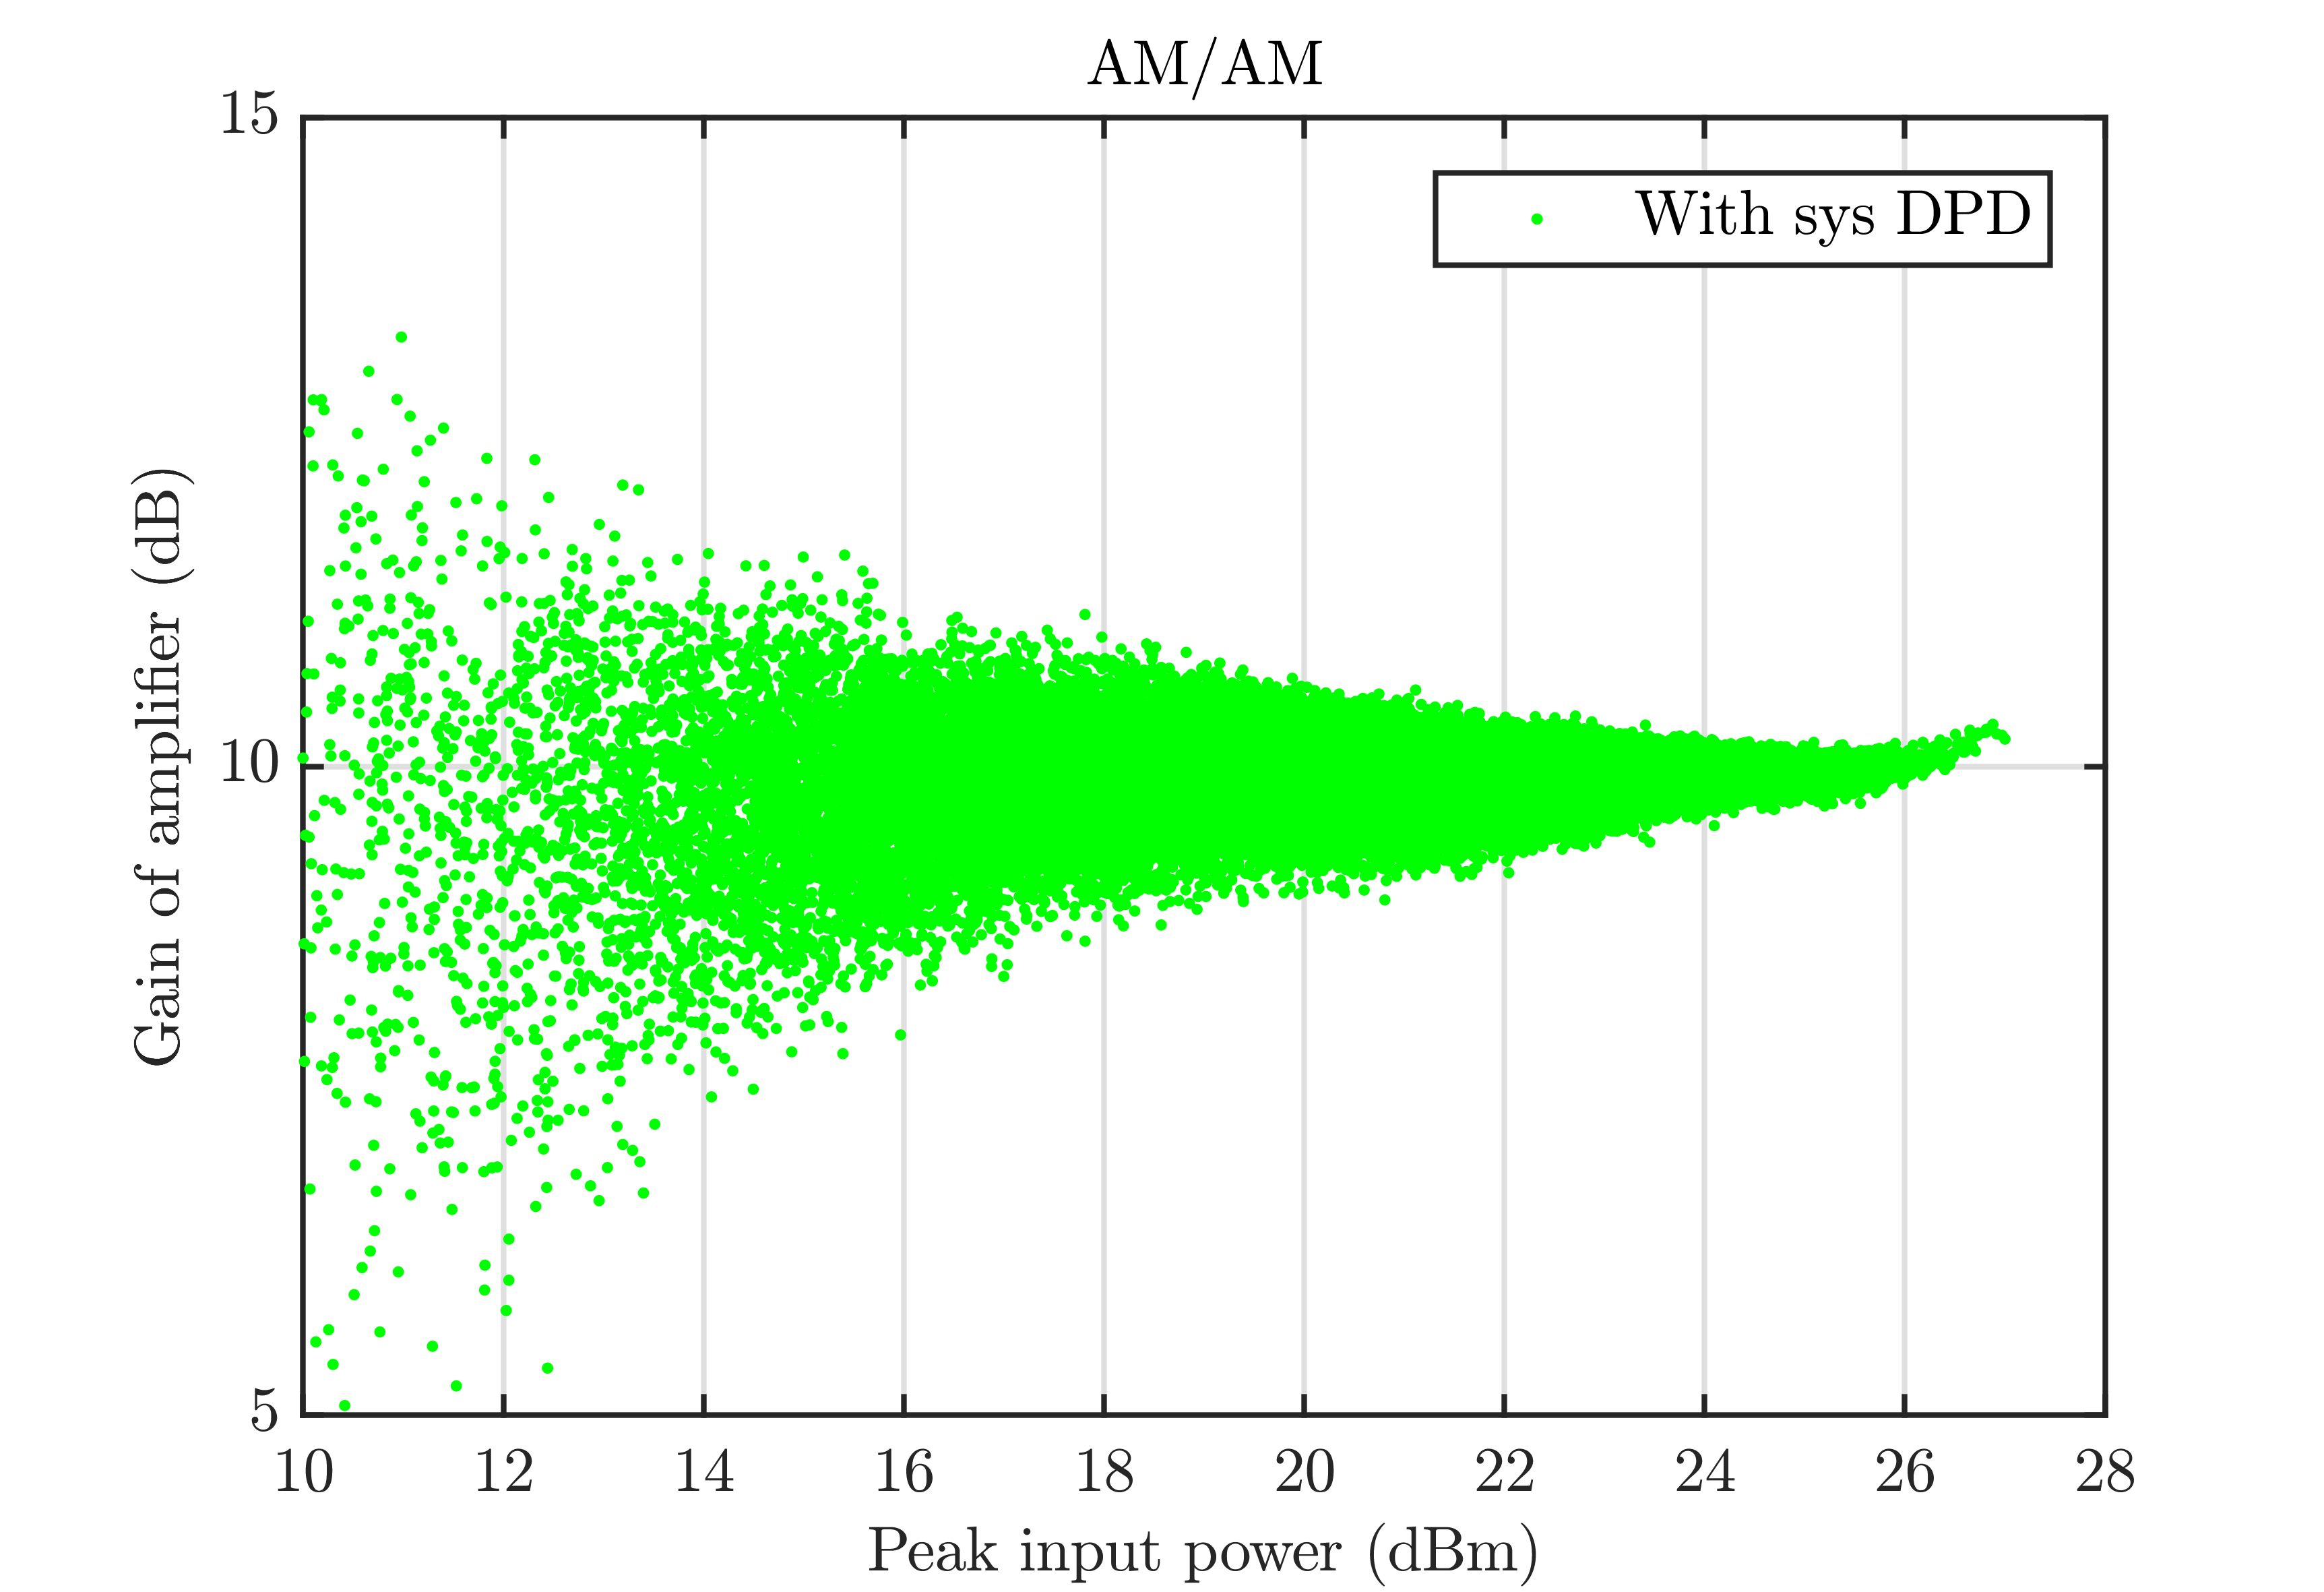
\includegraphics[scale = 0.5]{figures/measurement/cree/meas3/amam_sys_dpd_0p4.png}
	\caption{AM/AM distortion at $d = 0.4\lambda$ with system DPD}
    \label{fig:meas4_amam8}
  \end{minipage}
\end{figure}

\begin{figure}[H]
  \centering
  \begin{minipage}[b]{0.5\textwidth}
	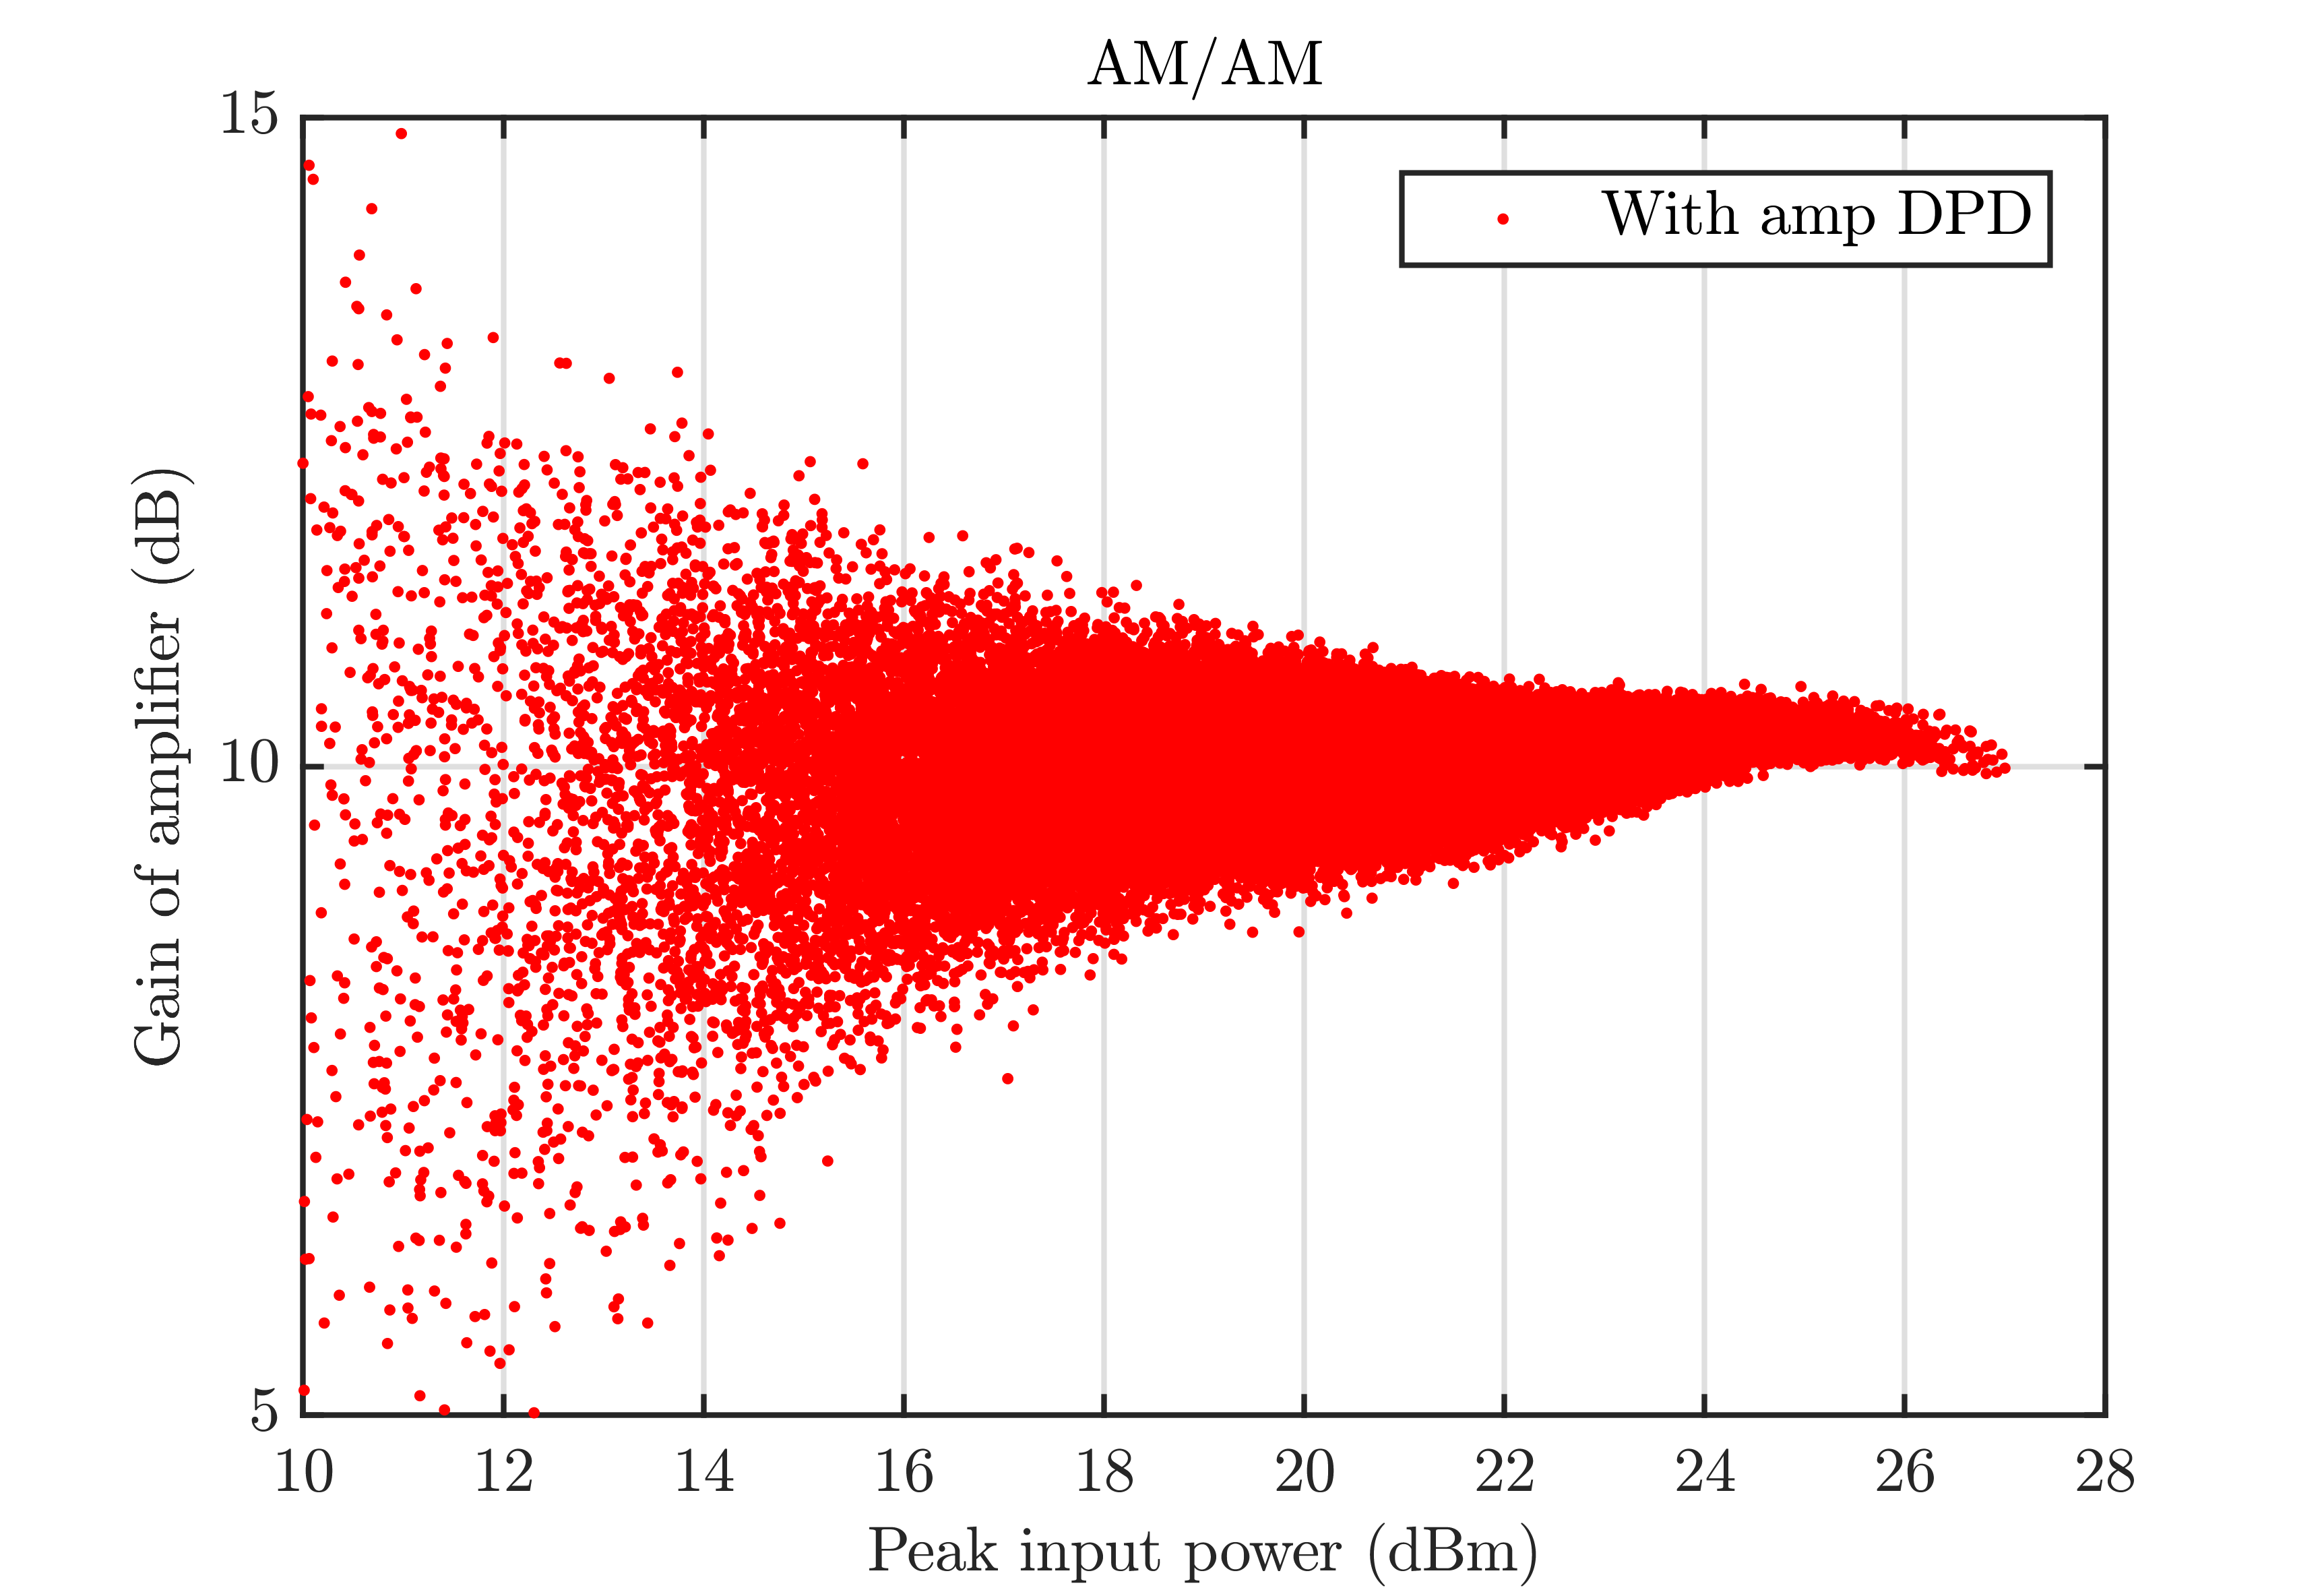
\includegraphics[scale = 0.5]{figures/measurement/cree/meas3/amam_amp_dpd_0p5.png}
	\caption{AM/AM distortion at $d = 0.5\lambda$ with amplifier DPD}	
    \label{fig:meas4_amam5_2}
  \end{minipage}
  \hfill
  \begin{minipage}[b]{0.4\textwidth}
	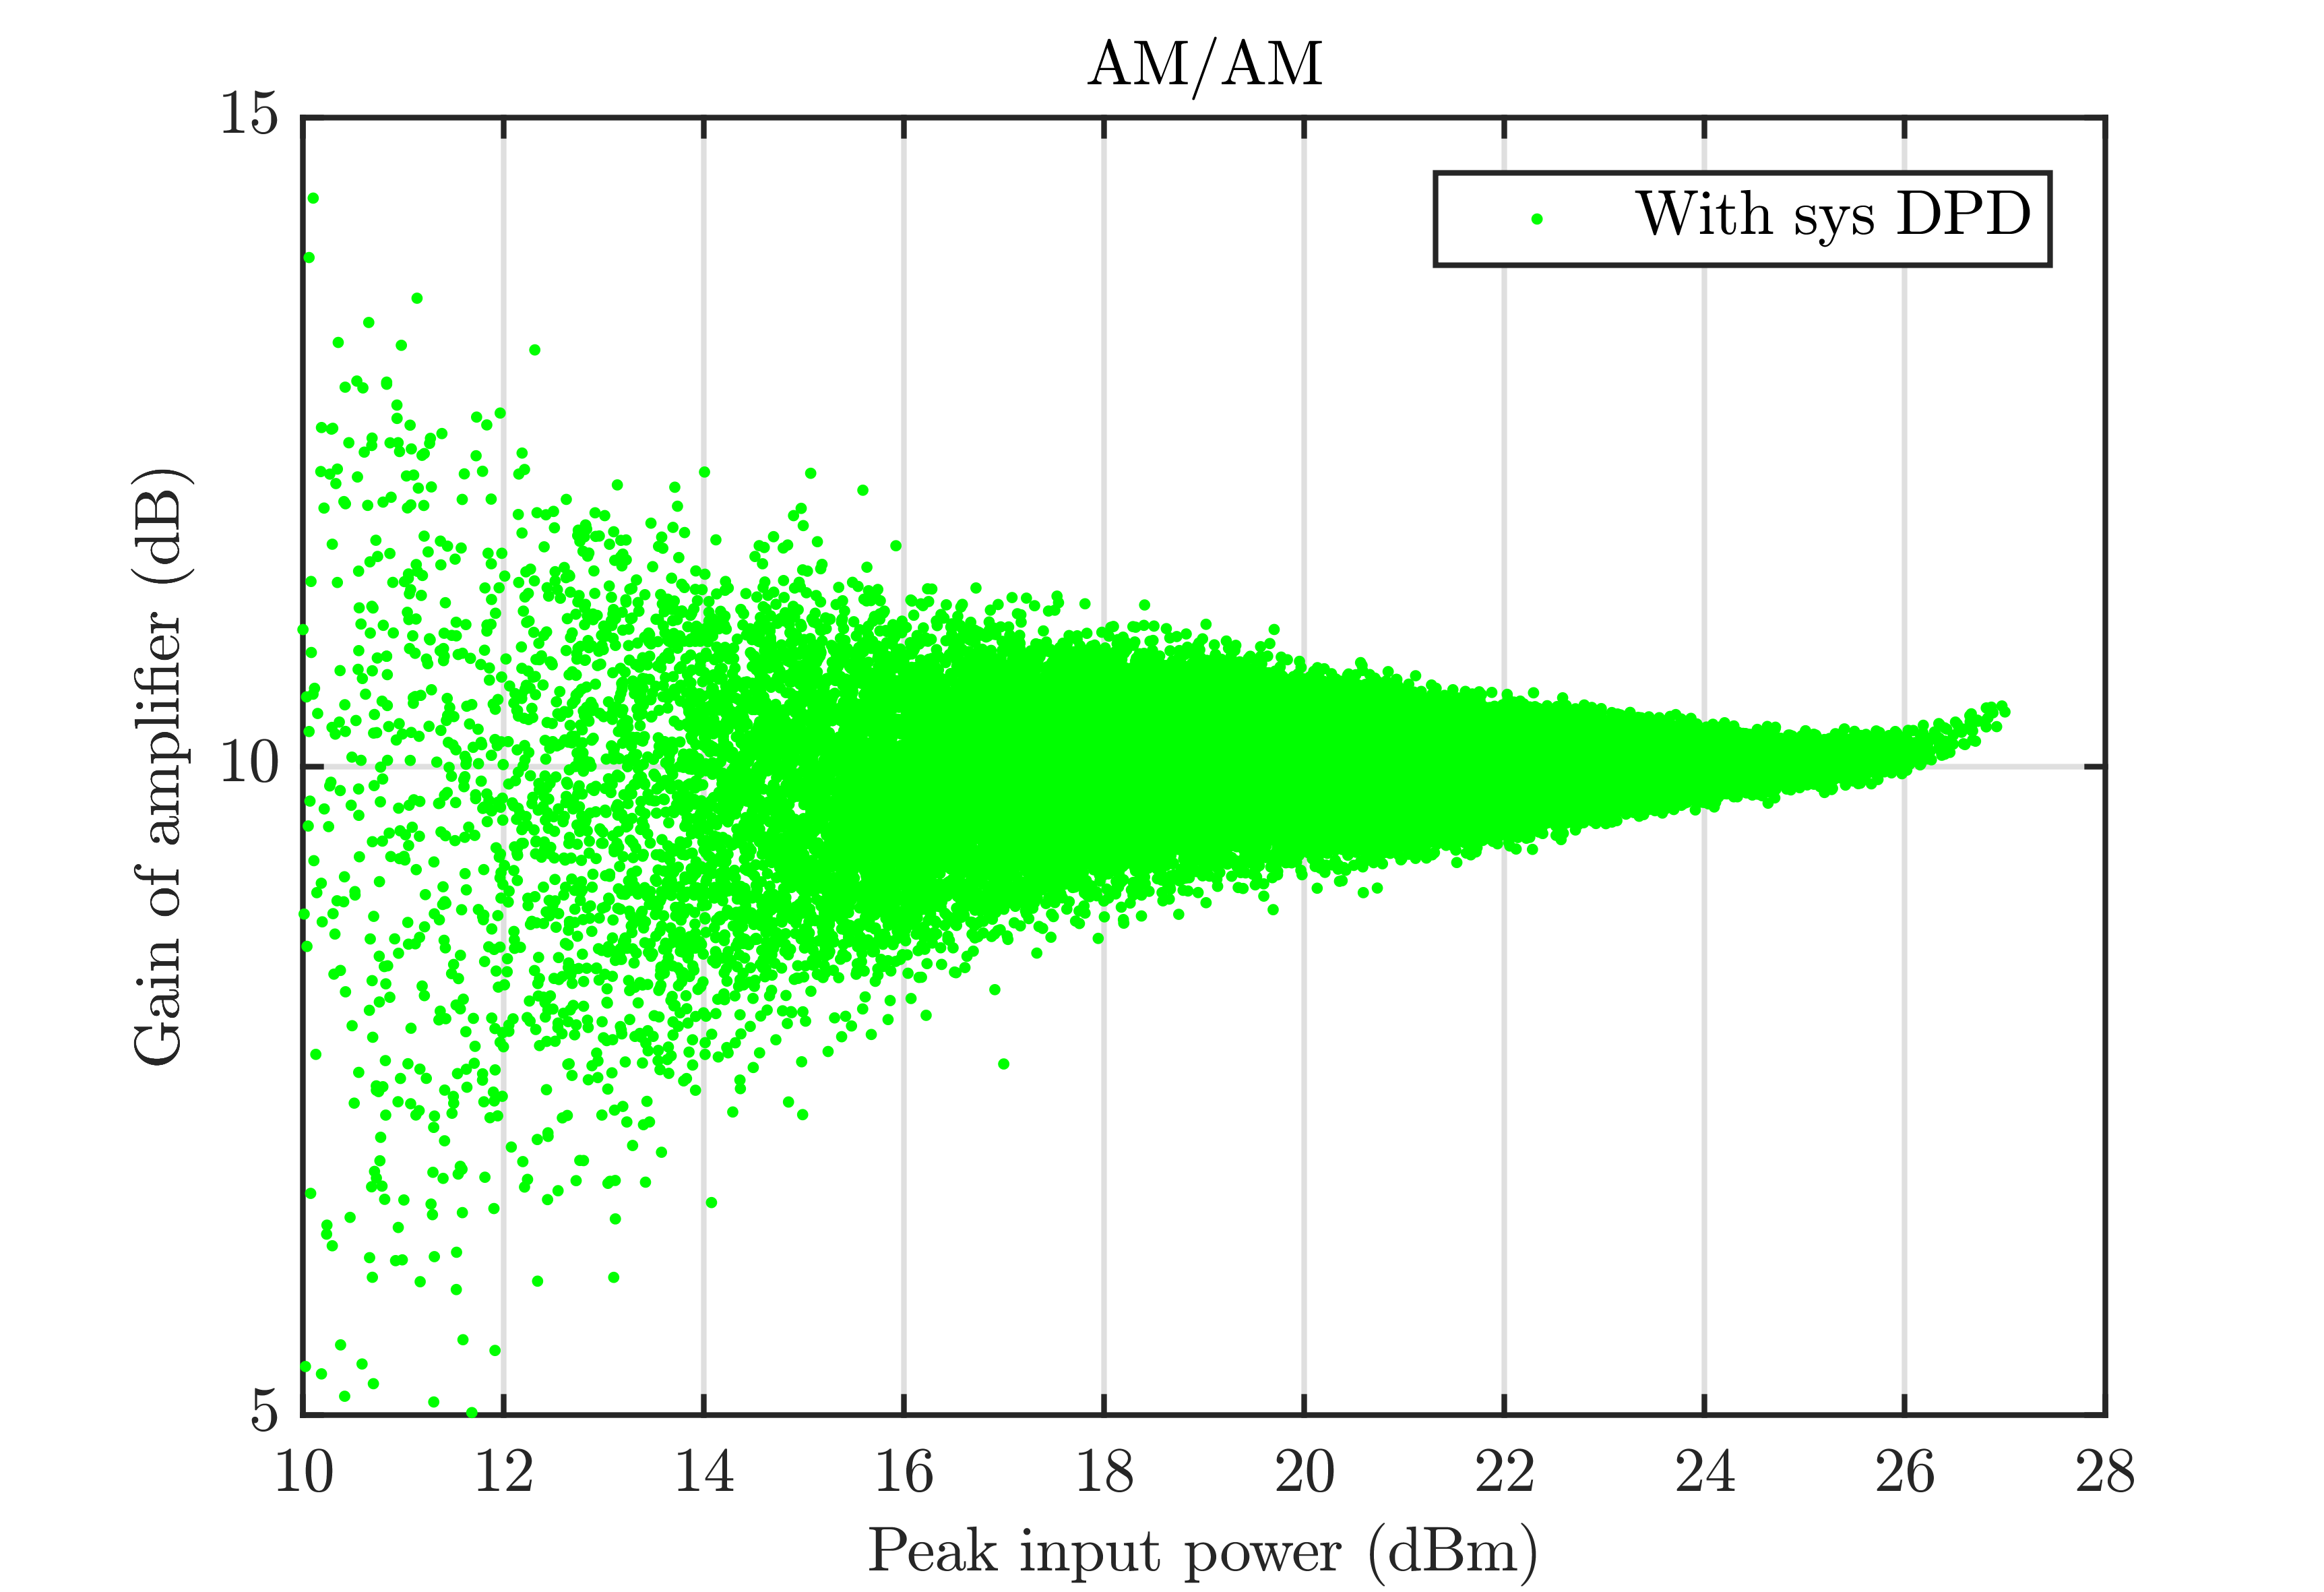
\includegraphics[scale = 0.5]{figures/measurement/cree/meas3/amam_sys_dpd_0p5.png}
	\caption{AM/AM distortion at $d = 0.5\lambda$ with system DPD}
    \label{fig:meas4_amam6_2}
  \end{minipage}
\end{figure}

\begin{figure}[H]
  \centering
  \begin{minipage}[b]{0.5\textwidth}
	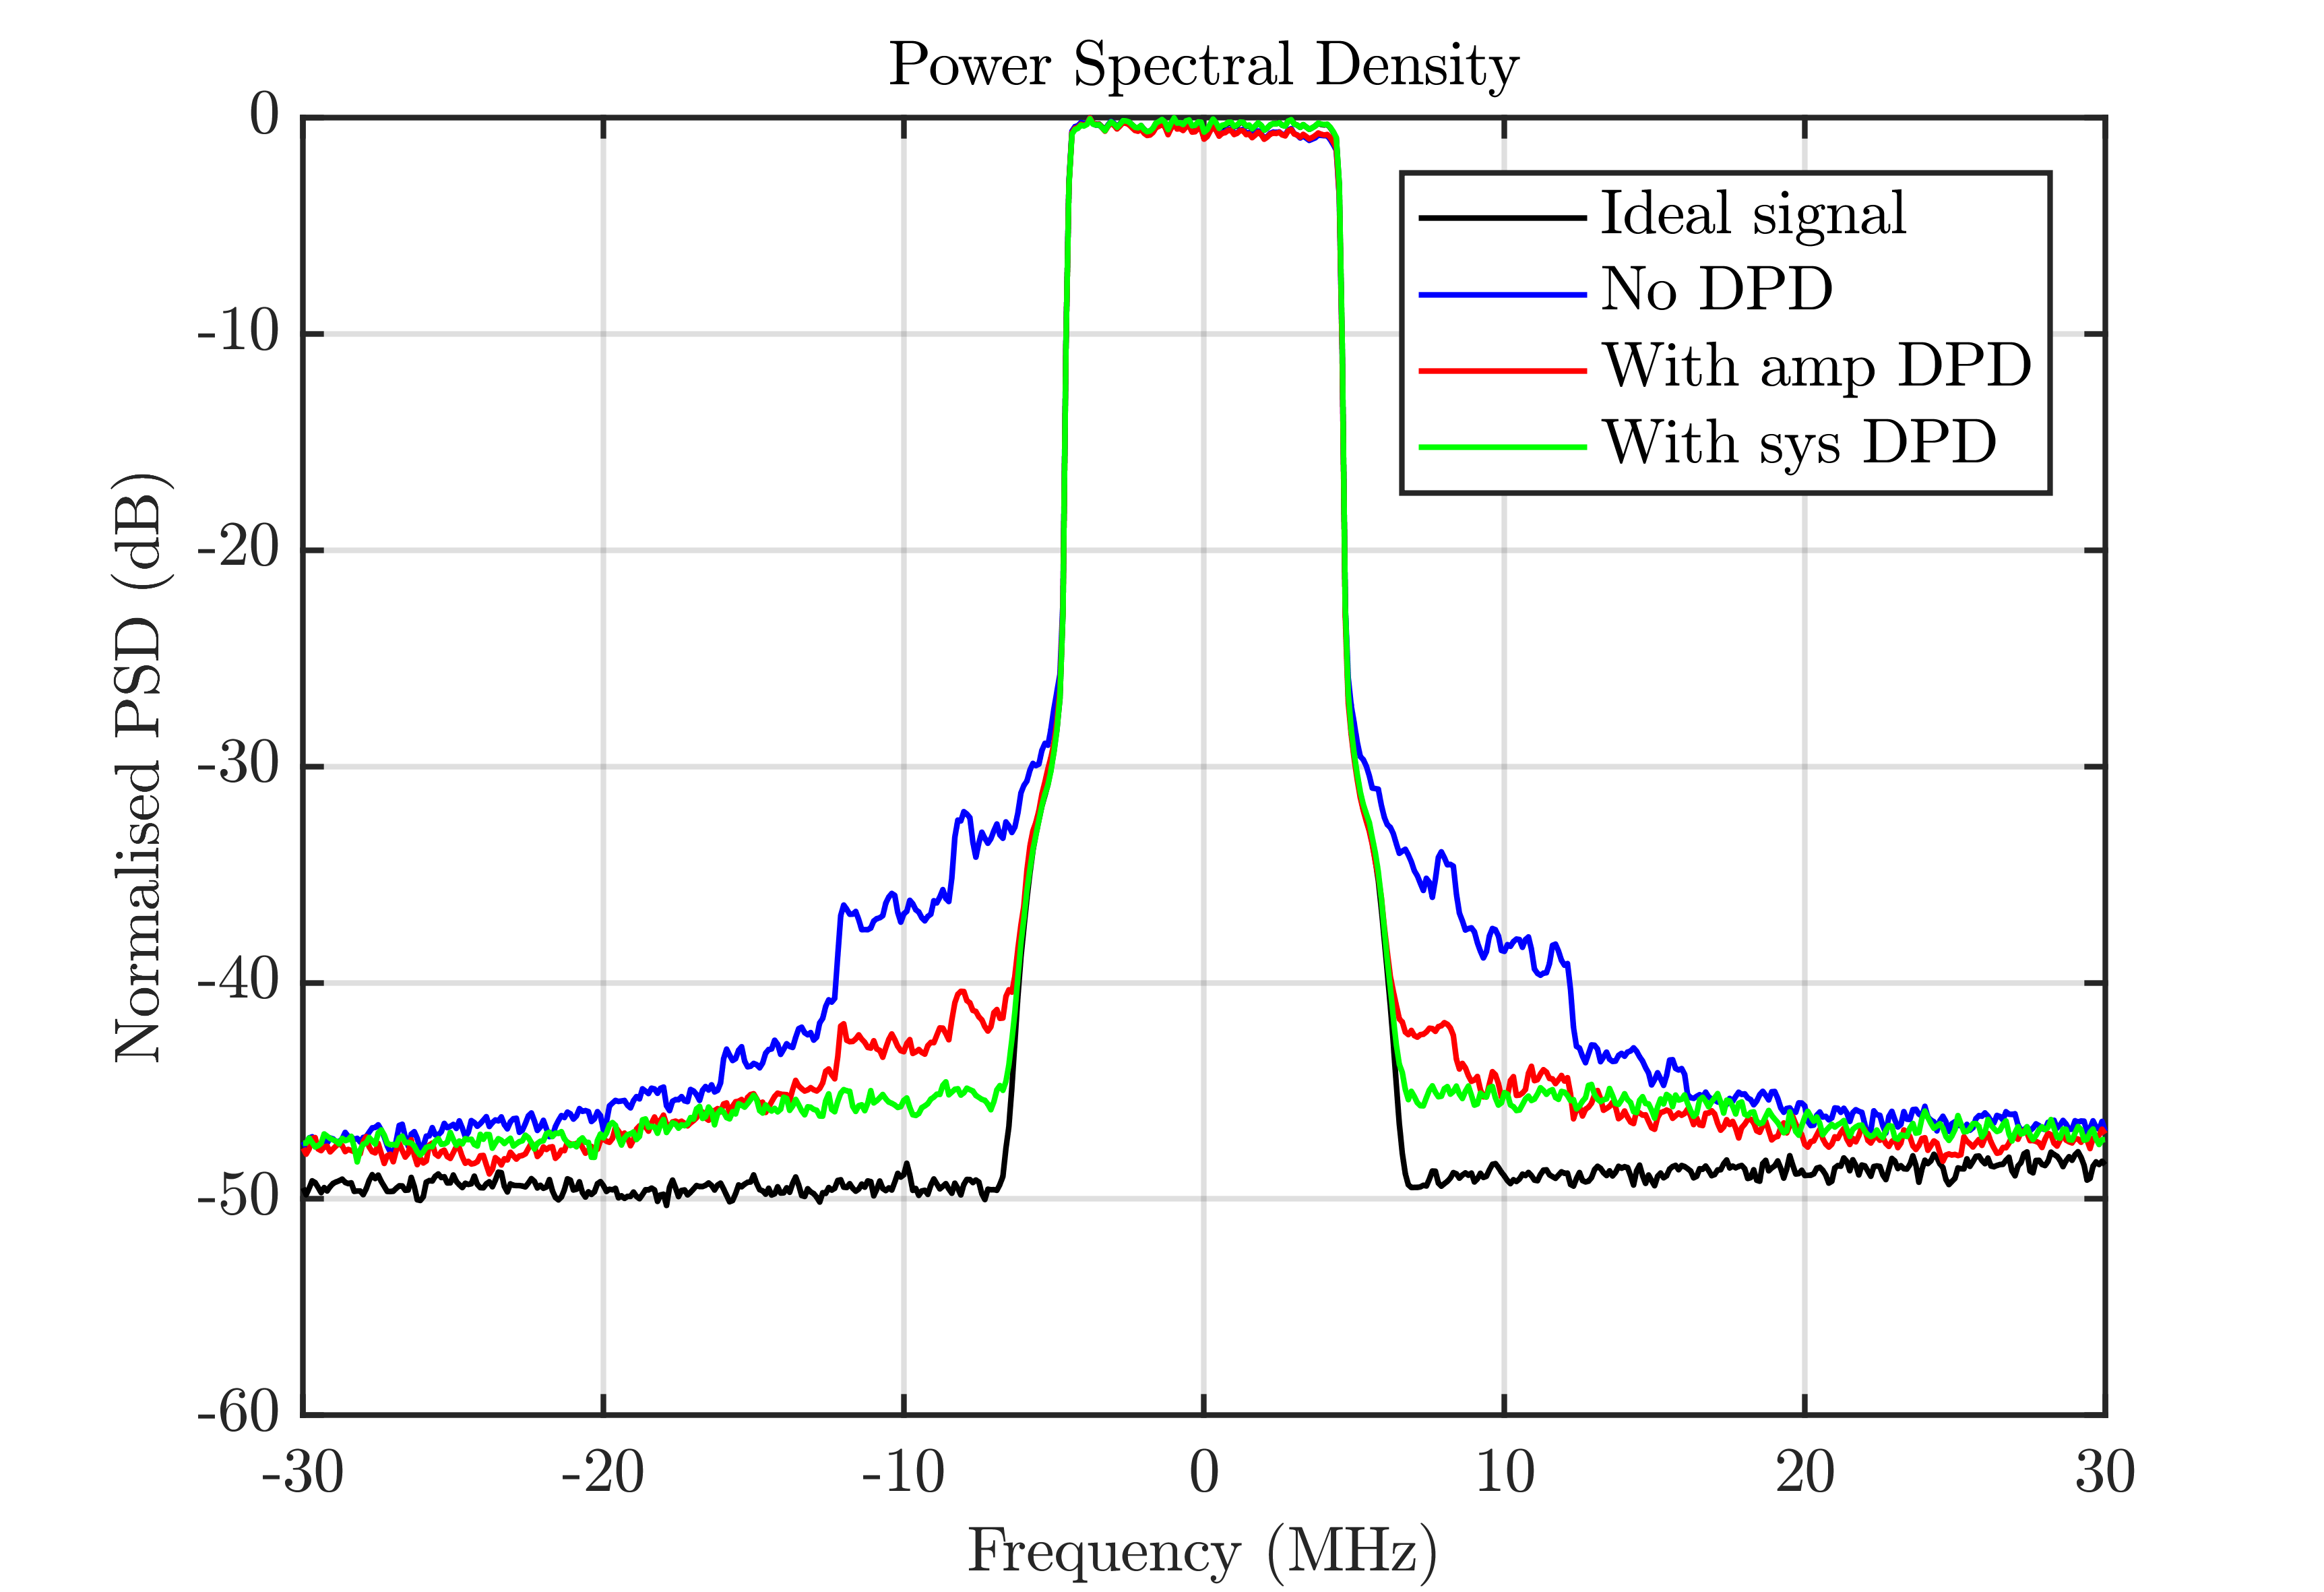
\includegraphics[scale = 0.5]{figures/measurement/cree/meas3/psd_0p5.png}
	\caption{PSD of measurement at $d = 0.5\lambda$ }	
    \label{fig:meas4_psd3_2}
  \end{minipage}
  \hfill
  \begin{minipage}[b]{0.4\textwidth}
	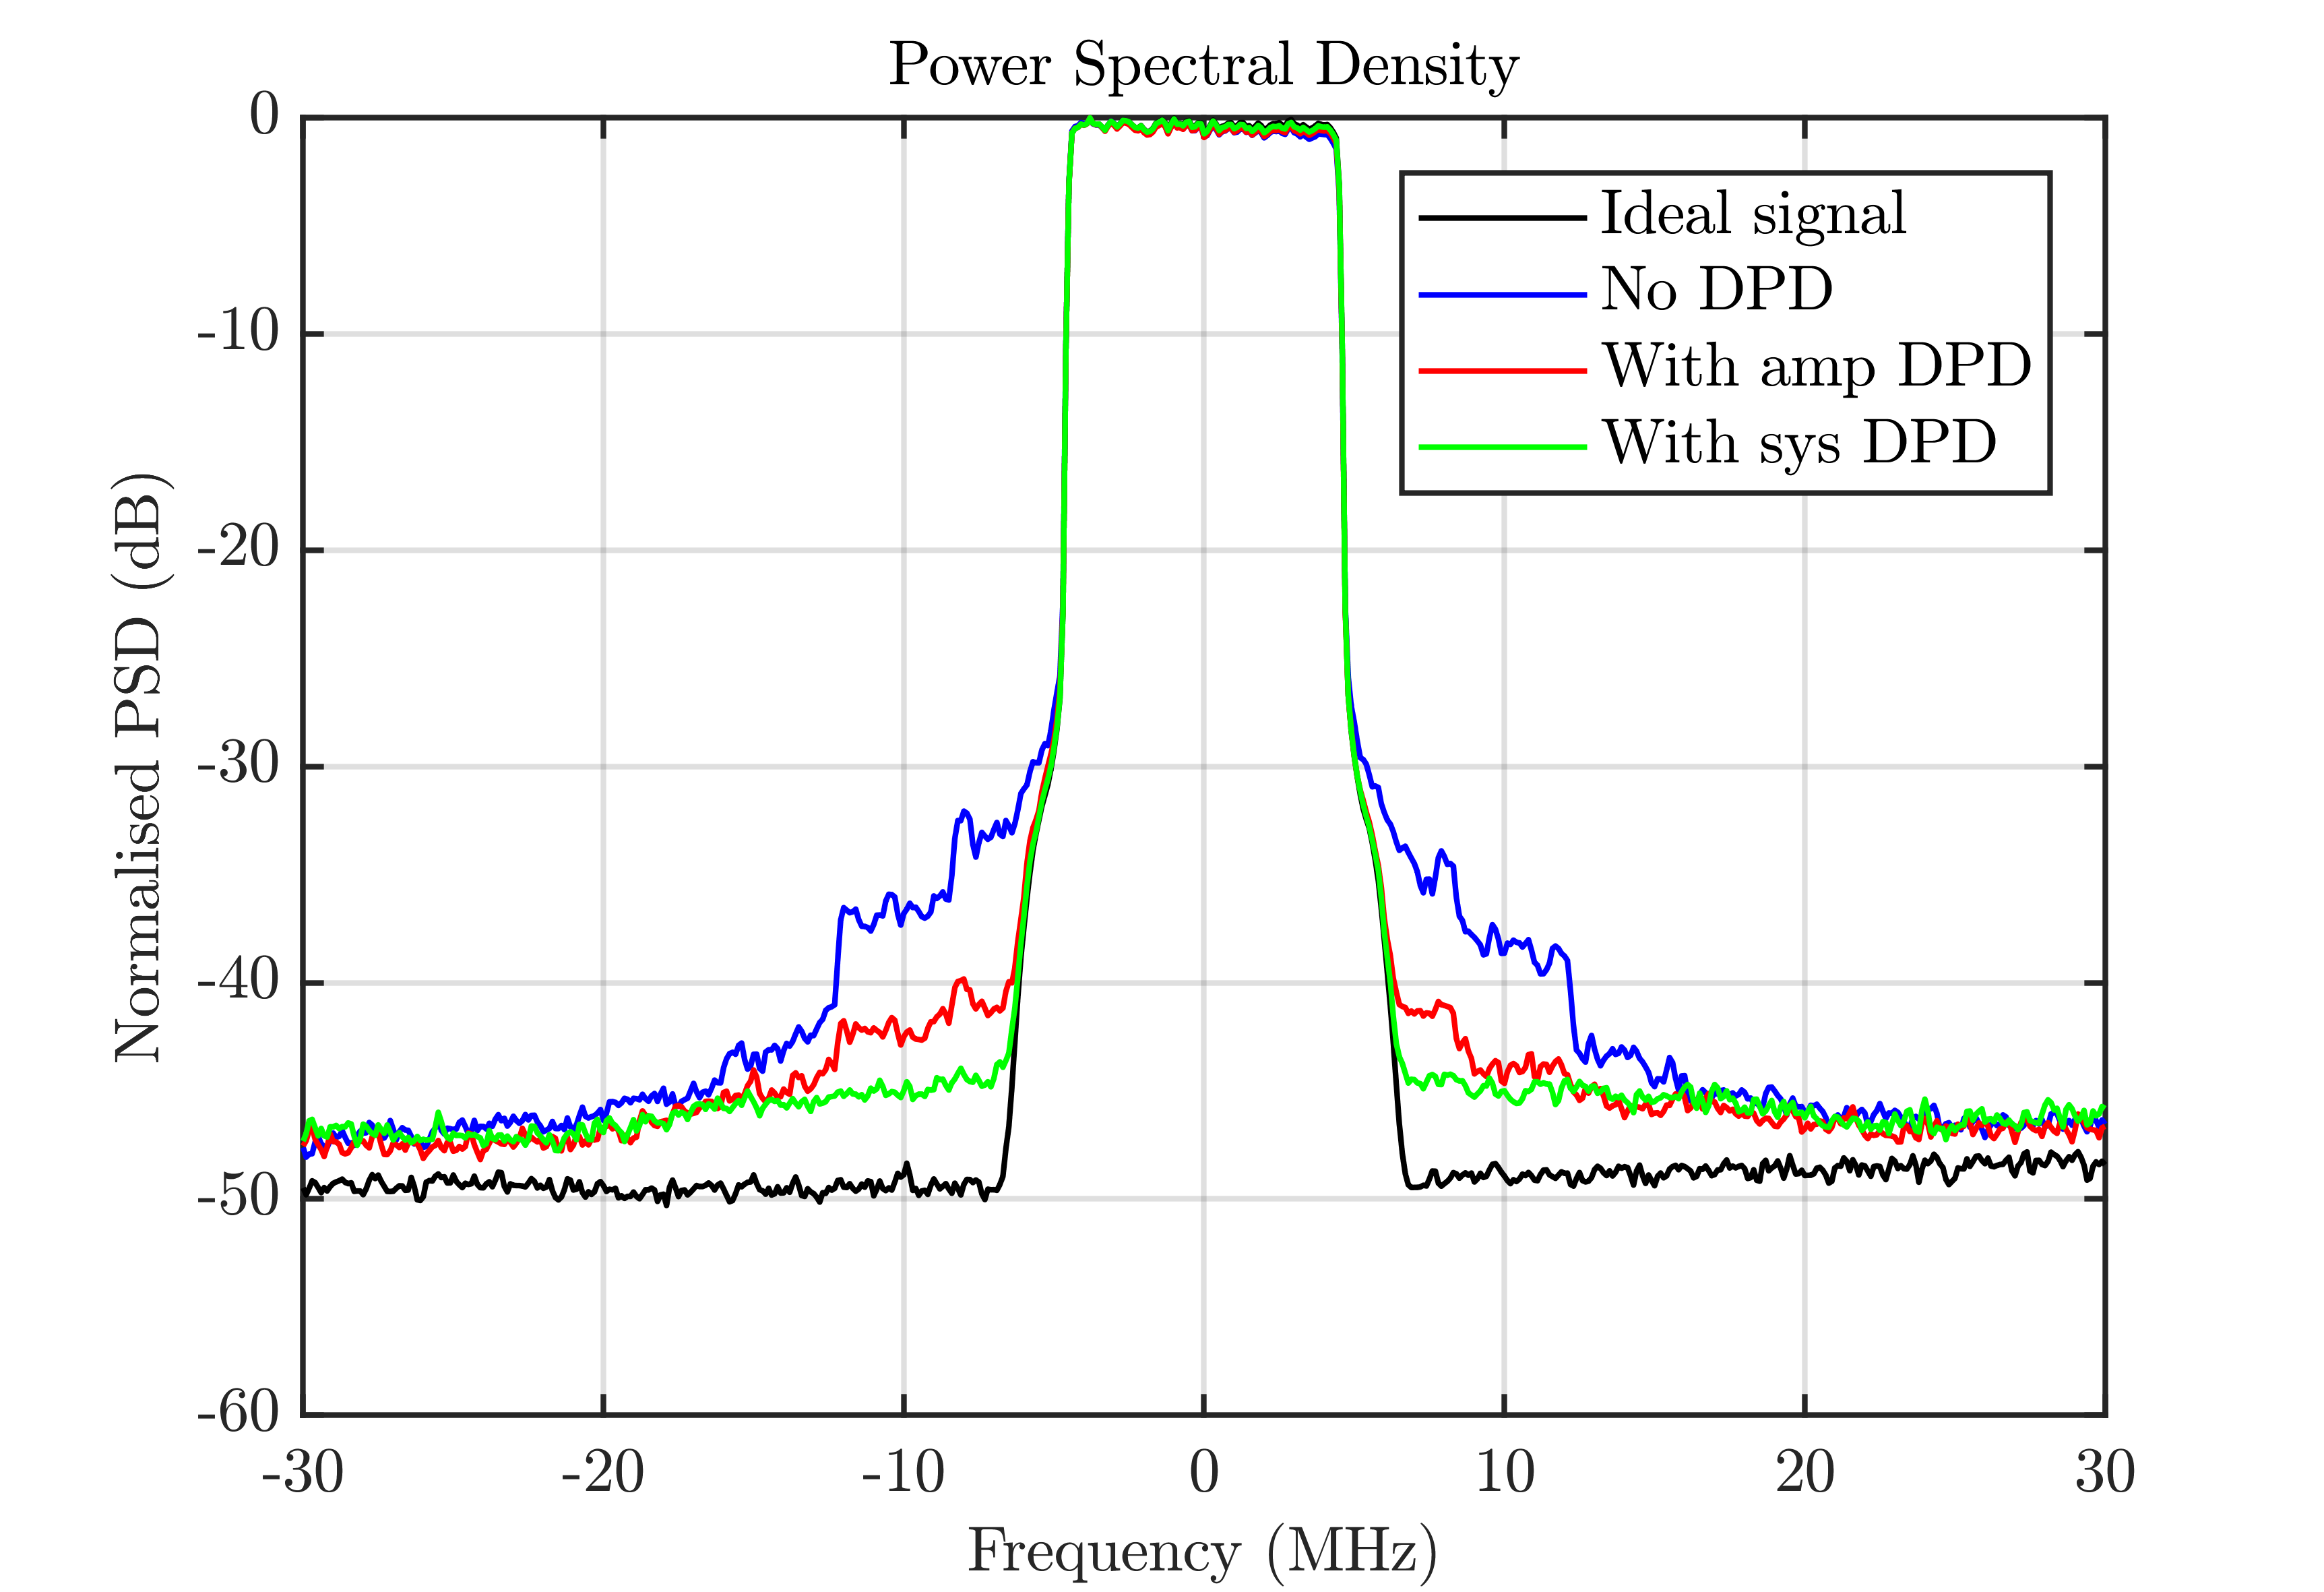
\includegraphics[scale = 0.5]{figures/measurement/cree/meas3/psd_0p6.png}
	\caption{PSD of measurement at $d = 0.6\lambda$}
    \label{fig:meas4_psd4_2}
  \end{minipage}
\end{figure}


\begin{figure}[H]
  \centering
  \begin{minipage}[b]{0.5\textwidth}
	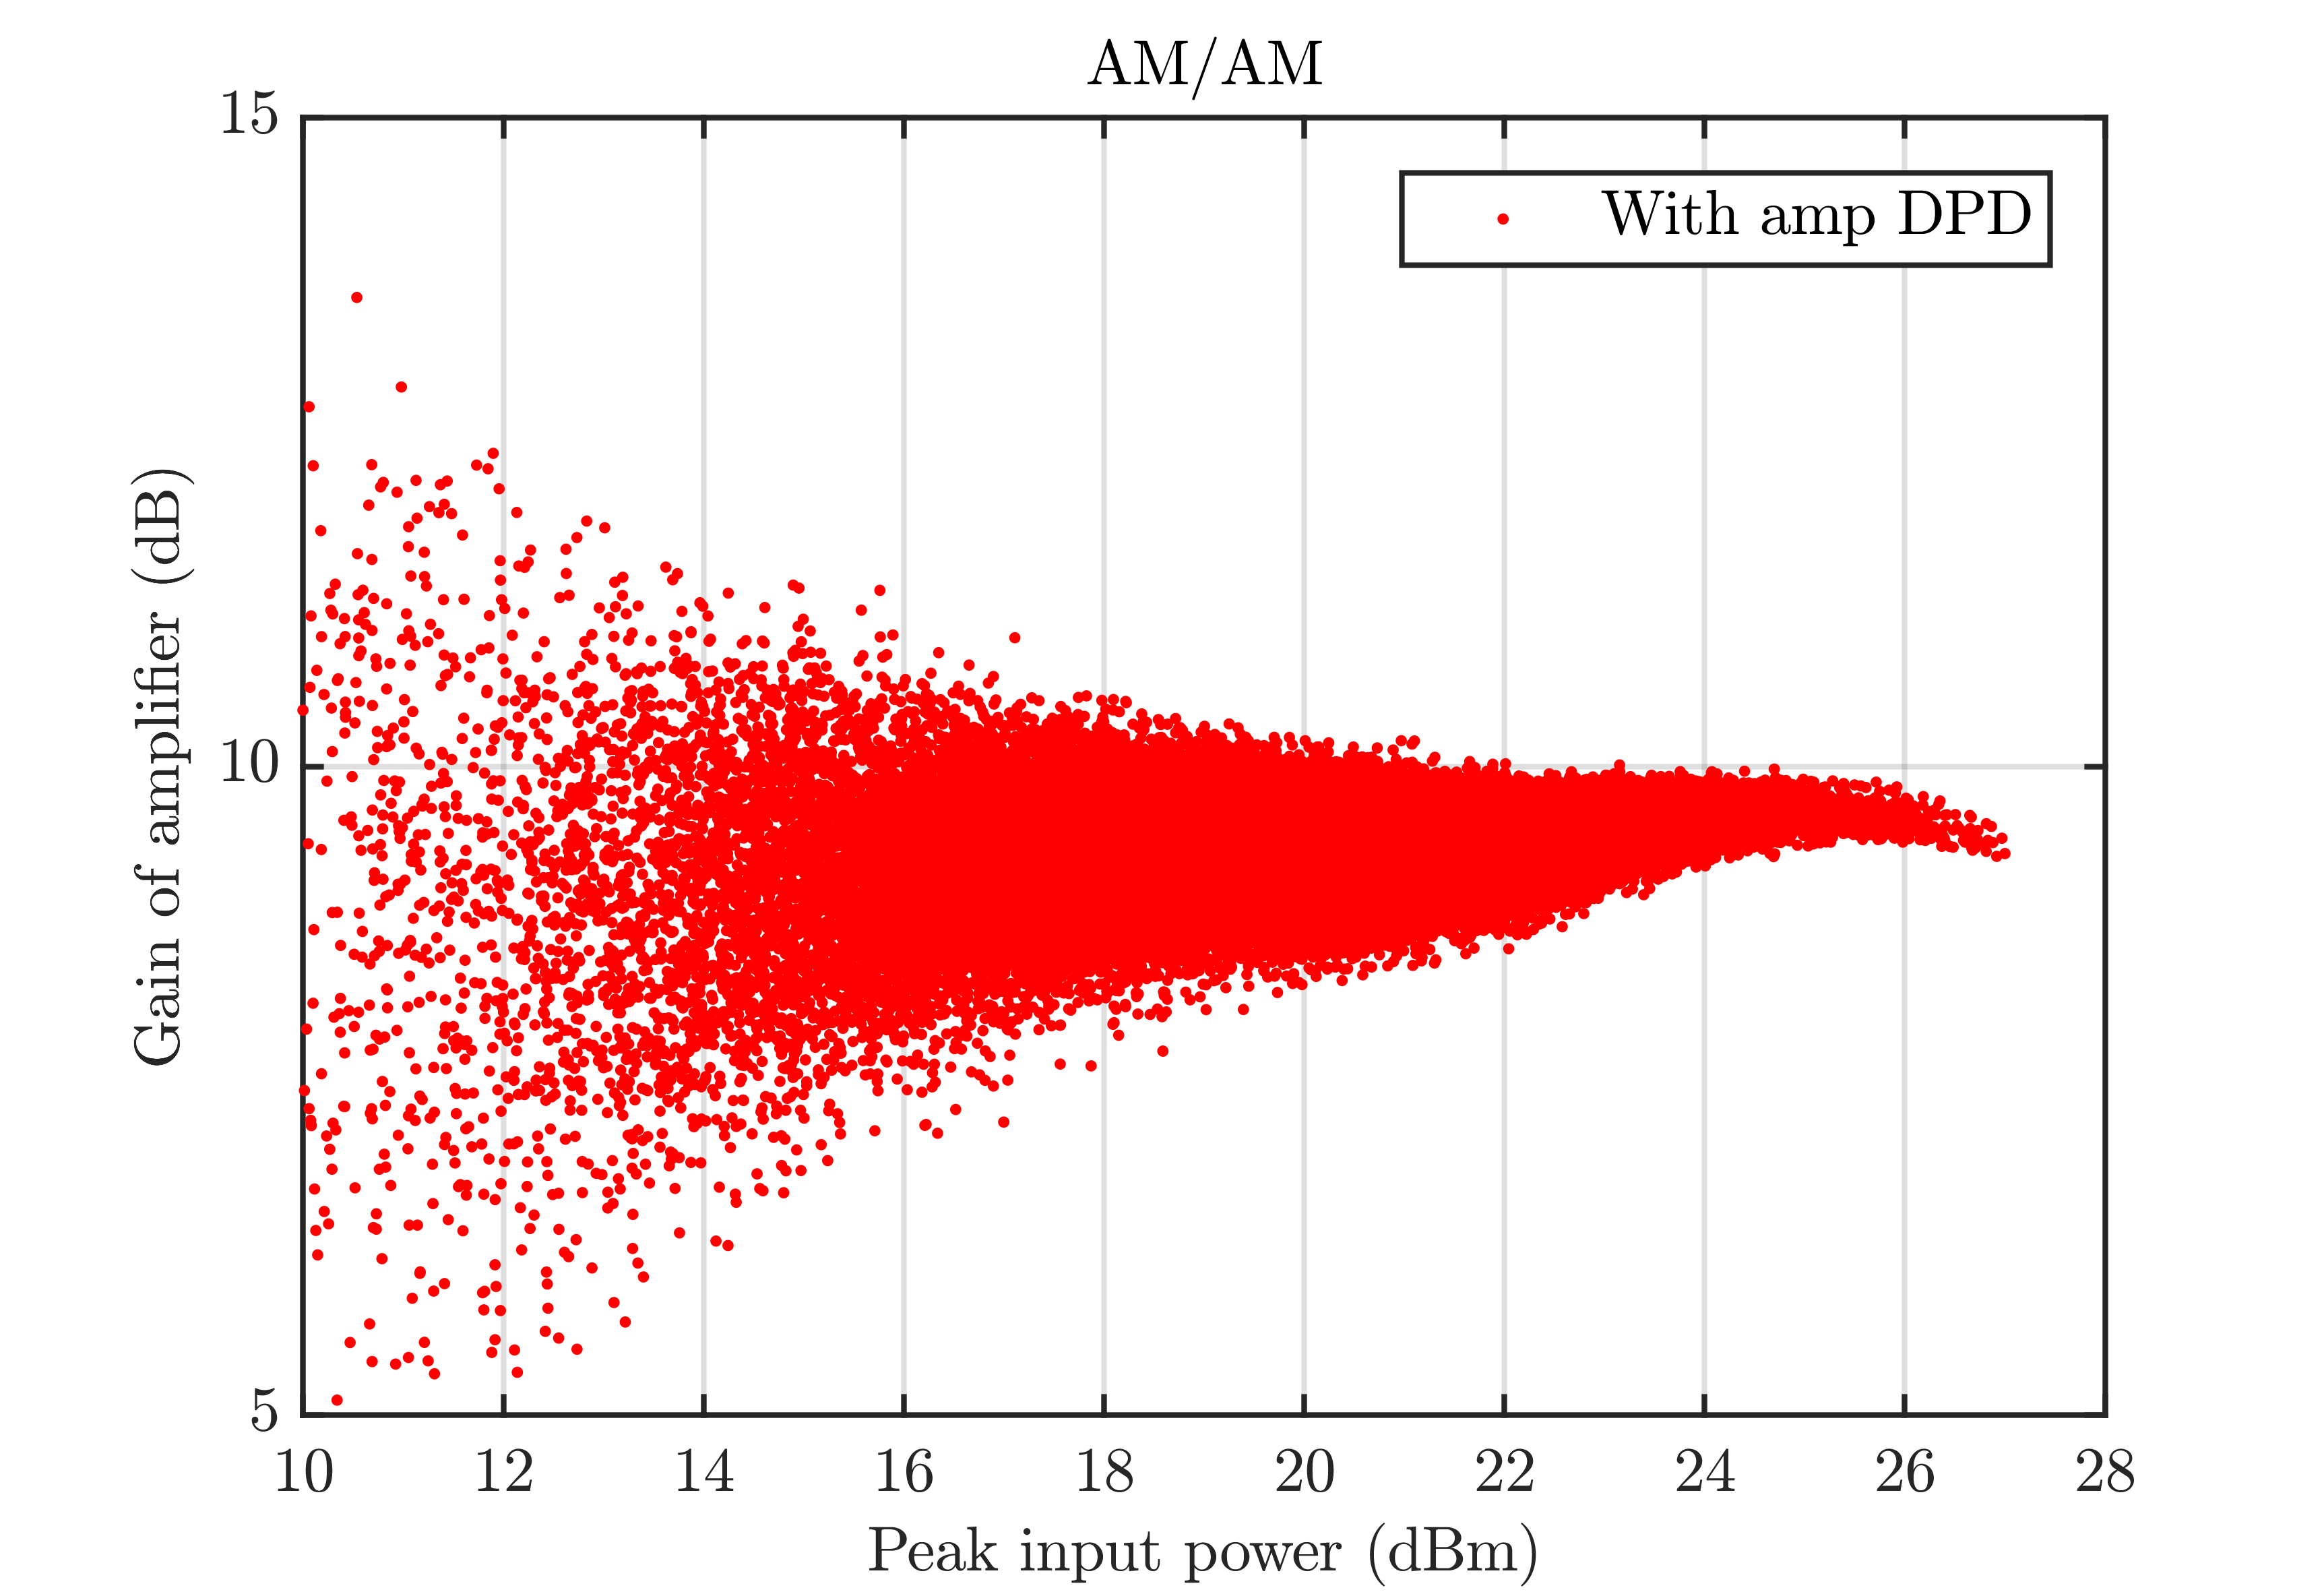
\includegraphics[scale = 0.5]{figures/measurement/cree/meas3/amam_amp_dpd_0p6.png}
	\caption{AM/AM distortion at $d = 0.6\lambda$ with amplifier DPD}	
    \label{fig:meas4_amam5_3}
  \end{minipage}
  \hfill
  \begin{minipage}[b]{0.4\textwidth}
	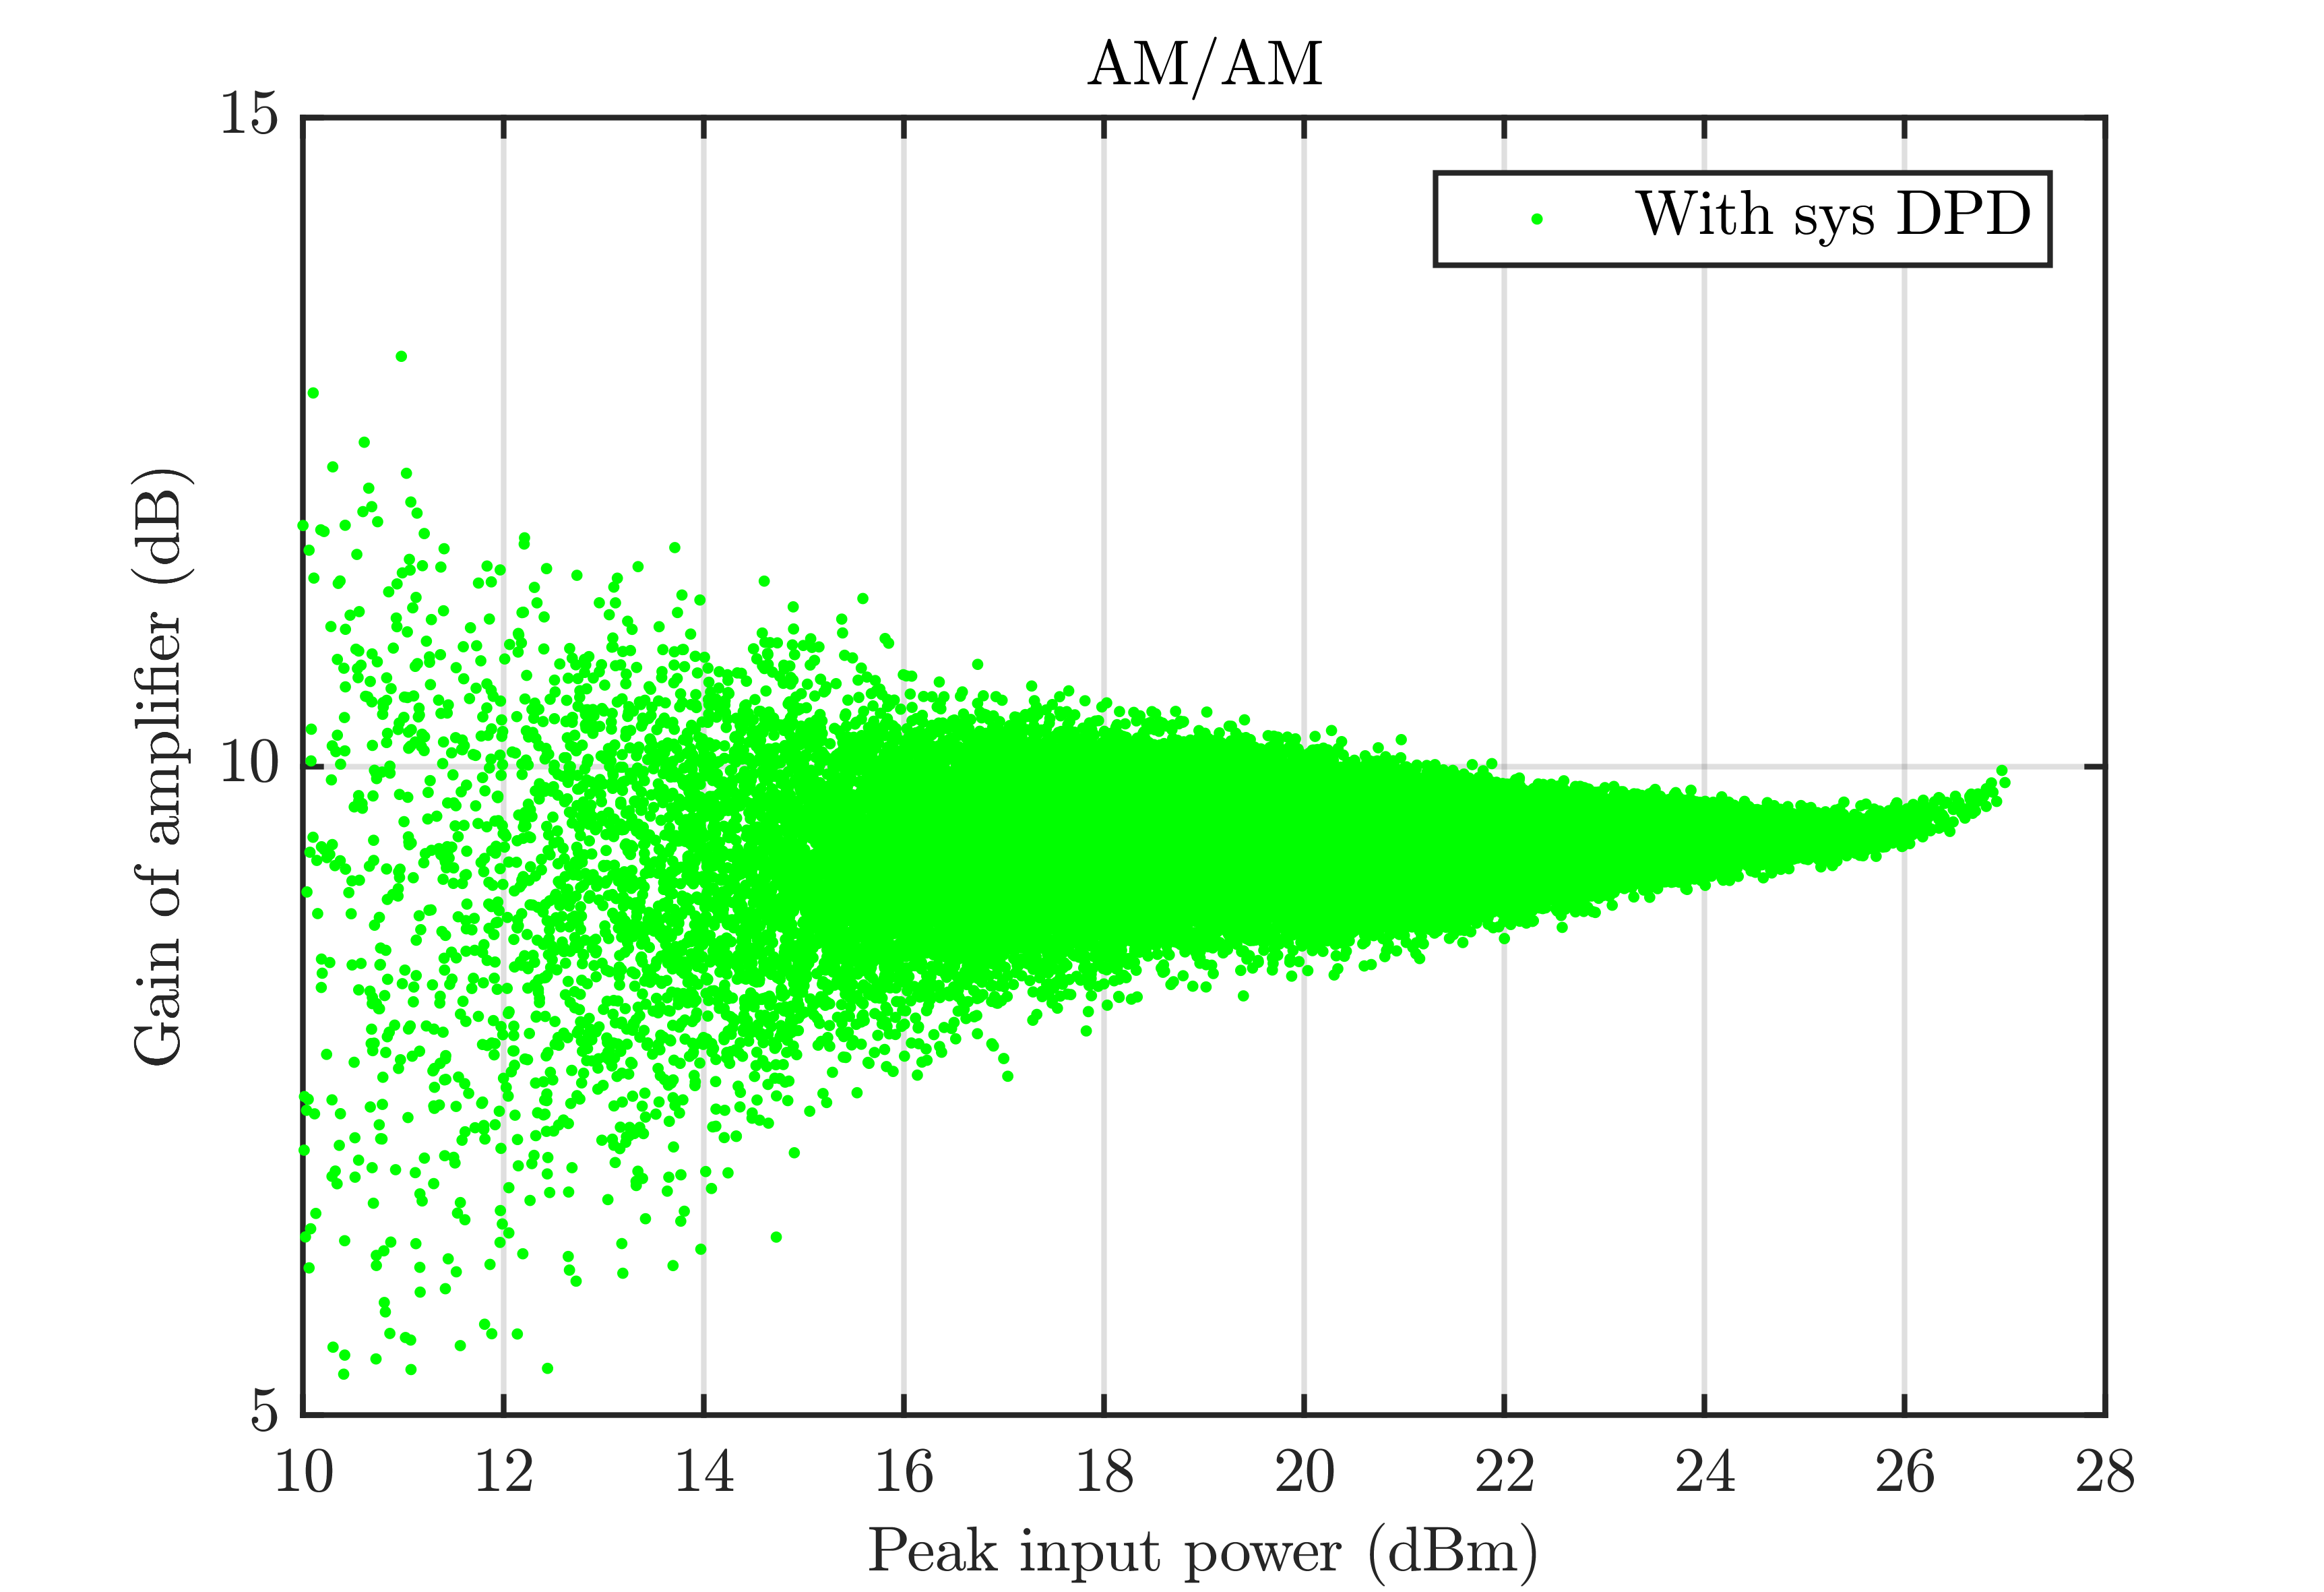
\includegraphics[scale = 0.5]{figures/measurement/cree/meas3/amam_sys_dpd_0p6.png}
	\caption{AM/AM distortion at $d = 0.6\lambda$ with system DPD}
    \label{fig:meas4_amam6_3}
  \end{minipage}
\end{figure}


\begin{figure}[H]
\centering 
\includegraphics[scale = 0.6]{figures/measurement/cree/meas4/acpr_four_ant.png}
\caption{ACPR versus distance between antennas}
\label{fig:meas4_dpd}
\end{figure}

It can be seen from figure \ref{fig:meas4_amam1} to \ref{fig:meas4_dpd} that the DPD algorithm still tends to overcompensate at high power values but still maintains a low ACPR. The ACPR is depicted in figure \ref{fig:meas4_dpd} and shows that the ACPR now changes more due to spacing in the antenna array, than in the case with two antennas. The lowest ACPR is found at $0.5\lambda$ like in the case with two antennas. Since the ACPR has the same shape in both cases for "Amp DPD" and "Sys DPD", a test has been made where the DPD model is obtained at $0.5\lambda$ and used at the other distances also. This was expected to make a large difference in the distortion since the S-parameters of the antennas changes a lot. See section \ref{ch:ant_meas} for antenna measurement. But from figure \ref{fig:meas4_amam5_4} and \ref{fig:meas4_amam6_4} it can be seen that the ACPR becomes somewhat linke the ACPR in figure \ref{fig:meas4_dpd}.

\begin{figure}[H]
  \centering
  \begin{minipage}[b]{0.5\textwidth}
	\includegraphics[scale = 0.5]{figures/measurement/cree/meas4/PSD_dif.png}
	\caption{PSD of measurement where the DPD model is obtained at 0.5$\lambda$ but is also used at other distances}	
    \label{fig:meas4_amam5_4}
  \end{minipage}
  \hfill
  \begin{minipage}[b]{0.4\textwidth}
	\includegraphics[scale = 0.5]{figures/measurement/cree/meas4/ACPR_dif.png}
	\caption{ACPR of measurement where the DPD model is obtained at 0.5$\lambda$ but is also used at other distances}
    \label{fig:meas4_amam6_4}
  \end{minipage}
\end{figure}



%%%%%%%%%%%%%%%%%%%%%%%%%%%%%%%%%%%%%%%%%%%%%%%%%%%%%%%%%%%%%%%%%%%%%%%%%%%%%%%%%%%%%%%%%%%%%%%%%%%%%%%%%%%%%%


\section{Two amplifiers different current}
In the former measurement the drain current for each amplifier has been adjusted to 100mA by tuning the gate voltage, to ensure same working conditions for all four amplifiers. In this section it is measured if it has any impact that the current is different. First all four amplifiers is connected to the same gate voltage and the current is measured in each amplifier. The two amplifiers with the largest difference is then used for these measurement. The results are shown in figure \ref{fig:meas5_1} to \ref{fig:meas5_9} which shows that when the gate voltage is ajusted the performance of the amplifiers changes. This is seen at the AM/AM plots where a difference clearly is seen. This is also why DPD with only considering one amplifier as a model not can be used for multiple amplifiers if the current is different. The results shows thou that if the amplifiers with antennas are treated as a hole, then the DPD algorithm works well and therefore a different bias current is not a huge problem when doing so.


\begin{figure}[H]
  \centering
  \begin{minipage}[b]{0.5\textwidth}
	\includegraphics[scale = 0.5]{figures/measurement/cree/meas5/amam_no_dpd_2p798v.png}
	\caption{AM/AM distortion at 56mA in amplifier 1 and 100mA in amplifier 2 with gate voltages at -2.798V without DPD}	
    \label{fig:meas5_1}
  \end{minipage}
  \hfill
  \begin{minipage}[b]{0.4\textwidth}
	\includegraphics[scale = 0.5]{figures/measurement/cree/meas5/amam_sys_dpd_2p798v.png}
	\caption{AM/AM distortion at 56mA in amplifier 1 and 100mA in amplifier 2 with gate voltages at -2.798V with DPD}
    \label{fig:meas5_1}
  \end{minipage}
\end{figure}
 
\begin{figure}[H]
  \centering
  \begin{minipage}[b]{0.5\textwidth}
	\includegraphics[scale = 0.5]{figures/measurement/cree/meas5/psd_2p798v.png}
	\caption{PSD at 56mA in amplifier 1 and 100mA in amplifier 2 with gate voltages at -2.798V}	
    \label{fig:meas5_3}
  \end{minipage}
  \hfill
  \begin{minipage}[b]{0.4\textwidth}
	\includegraphics[scale = 0.5]{figures/measurement/cree/meas5/amam_no_dpd_2p742v.png}
	\caption{AM/AM distortion at 75mA in amplifier 1 and 112mA in amplifier 2 with gate voltages at -2.742V without DPD}
    \label{fig:meas5_4}
  \end{minipage}
\end{figure}

\begin{figure}[H]
  \centering
  \begin{minipage}[b]{0.5\textwidth}
	\includegraphics[scale = 0.5]{figures/measurement/cree/meas5/amam_sys_dpd_2p742v.png}
	\caption{AM/AM distortion at 75mA in amplifier 1 and 112mA in amplifier 2 with gate voltages at -2.742V with DPD}	
    \label{fig:meas5_5}
  \end{minipage}
  \hfill
  \begin{minipage}[b]{0.4\textwidth}
	\includegraphics[scale = 0.5]{figures/measurement/cree/meas5/psd_2p742v.png}
	\caption{PSD at 75mA in amplifier 1 and 112mA in amplifier 2 with gate voltages at -2.742V}
    \label{fig:meas5_6}
  \end{minipage}
\end{figure}


\begin{figure}[H]
  \centering
  \begin{minipage}[b]{0.5\textwidth}
	\includegraphics[scale = 0.5]{figures/measurement/cree/meas5/amam_no_dpd_2p672v.png}
	\caption{AM/AM distortion at 100mA in amplifier 1 and 136mA in amplifier 2 with gate voltages at -2.672V without DPD}	
    \label{fig:meas5_7}
  \end{minipage}
  \hfill
  \begin{minipage}[b]{0.4\textwidth}
	\includegraphics[scale = 0.5]{figures/measurement/cree/meas5/amam_sys_dpd_2p672v.png}
	\caption{AM/AM distortion at 100mA in amplifier 1 and 137mA in amplifier 2 with gate voltages at -2.672V with DPD}
    \label{fig:meas5_8}
  \end{minipage}
\end{figure}


\begin{figure}[H]
\centering 
\includegraphics[scale = 0.5]{figures/measurement/cree/meas5/psd_2p672v.png}
\caption{PSD at 100mA in amplifier 1 and 137mA in amplifier 2 with gate voltages at -2.672V}
\label{fig:meas5_9}
\end{figure}





 

